% !TeX encoding = UTF-8
% !TeX spellcheck = es_AR
% arara: pdflatex
% arara: makeindex: { style: biblioteca/thebook_indexstyle }
% arara: biber
% arara: pdflatex
% arara: pdflatex
% arara: pdflatex

%%%%%%%%%%%%%%%%%%%%%%%%%%%%%%%%%%%%%%%%%
% Solucionario del Cuadernillo de Elementos de Programación y Lógica
% Universidad Nacional de Quilmes
% Version 0.6.0 (24/04/2022)
%
% Original Author:
% Alan Rodas Bonjour (alanrodas@gmail.com)
%
% Based on "The Legrand Orange Book" by
% Mathias Legrand (legrand.mathias@gmail.com)
% with modifications by:
% Vel (vel@latextemplates.com)
%
% License:
% CC BY-NC-SA 3.0 (http://creativecommons.org/licenses/by-nc-sa/3.0/)
%
% Compiling this template:
% This template uses biber for its bibliography and makeindex for its index.
% When you first open the template, compile it from the command line with the
% commands below to make sure your LaTeX distribution is configured correctly:
%
% 1) pdflatex main
% 2) makeindex main.idx -s StyleInd.ist
% 3) biber main
% 4) pdflatex main x 2
%
% After this, when you wish to update the bibliography/index use the appropriate
% command above and make sure to compile with pdflatex several times
% afterwards to propagate your changes to the document.
%
% Alternatively you can use the "arara" building tool to build this
% document, by wunning "arara main"
%
% This template also uses a number of packages which may need to be
% updated to the newest versions for the template to compile. It is strongly
% recommended you update your LaTeX distribution if you have any
% compilation errors.
%
% Important note:
% Chapter heading images should have a 2:1 width:height ratio,
% e.g. 920px width and 460px height.
%
%%%%%%%%%%%%%%%%%%%%%%%%%%%%%%%%%%%%%%%%%

%----------------------------------------------------------------------------------------
%	PACKAGES AND OTHER DOCUMENT CONFIGURATIONS
%----------------------------------------------------------------------------------------

\documentclass[11pt,fleqn]{book} % Default font size and left-justified equations

%----------------------------------------------------------------------------------------

%%%%%%%%%%%%%%%%%%%%%%%%%%%%%%%%%%%%%%%%%
% The Legrand Orange Book
% Structural Definitions File
% Version 3.0 (18/09/2018)
%
% Original author:
% Mathias Legrand (legrand.mathias@gmail.com)
% with modifications by:
% Vel (vel@latextemplates.com)
% with modifications by:
% Alan Rodas Bonjour (alanrodas@gmail.com)
%
% This file has been downloaded from:
% http://www.LaTeXTemplates.com
%
% License:
% CC BY-NC-SA 3.0 (http://creativecommons.org/licenses/by-nc-sa/3.0/)
%
%%%%%%%%%%%%%%%%%%%%%%%%%%%%%%%%%%%%%%%%%

%----------------------------------------------------------------------------------------
%	VARIOUS REQUIRED PACKAGES AND CONFIGURATIONS
%----------------------------------------------------------------------------------------

\usepackage[dvipsnames]{xcolor} % Required for specifying colors by name

\usepackage[top=3cm,bottom=3cm,left=3cm,right=3cm,headsep=10pt,a4paper]{geometry} % Page margins
\usepackage{changepage}

\usepackage{graphicx} % Required for including pictures
\graphicspath{{Imagenes/}} % Specifies the directory where pictures are stored

\usepackage{lipsum} % Inserts dummy text

\usepackage{tikz} % Required for drawing custom shapes

\usepackage[spanish]{babel} % Spanish language/hyphenation

\usepackage[shortlabels]{enumitem} % Customize lists
\setlist{nolistsep} % Reduce spacing between bullet points and numbered lists

\usepackage{booktabs} % Required for nicer horizontal rules in tables

\usepackage[export]{adjustbox} % Allows changing character box alignment

\usepackage{wrapfig}

\usepackage{appendix}
\renewcommand{\appendixname}{Anexo}
\renewcommand{\appendixpagename}{Anexos}
\renewcommand{\appendixtocname}{Anexos}

\usepackage{listings} % Allow code environments with accents

\usepackage{xkeyval} % Allows key value parameters

\usepackage{enumitem} % Allows enumerations with preffix, suffix

%----------------------------------------------------------------------------------------
%	DEFAULT COLORS AND CODE STYLE
%----------------------------------------------------------------------------------------
\definecolor{primary}{RGB}{243,176,25} % Define the primary color used for highlighting throughout the book

\definecolor{codebase}{RGB}{0,0,0}
\definecolor{codecomments}{RGB}{0,120,0}
\definecolor{codekeywords}{RGB}{0,0,120}
\definecolor{codestrings}{RGB}{150,150,0}
\definecolor{codemorekeywords}{RGB}{200,50,50}

\lstset{
    basicstyle=\ttfamily\small,
    numberstyle=\footnotesize,
    numbers=left,
    backgroundcolor=\color{gray!10},
    frame=single,
    tabsize=2,
    rulecolor=\color{codebase!30},
    commentstyle=\color{codecomments},
    keywordstyle=\color{codekeywords},
    stringstyle=\color{codestrings},
    title=\lstname,
    escapeinside={\%(*}{*)},
    breaklines=true,
    breakatwhitespace=true,
    showstringspaces=false,
    framextopmargin=2pt,
    framexbottommargin=2pt,
    framexleftmargin=2pt,
    framexrightmargin=2pt,
    inputencoding=utf8,
    extendedchars=true,
    literate={á}{{\'a}}1 {é}{{\'e}}1 {í}{{\'i}}1 {ó}{{\'o}}1 {ú}{{\'u}}1
             {Á}{{\'A}}1 {É}{{\'E}}1 {Í}{{\'I}}1 {Ó}{{\'O}}1 {Ú}{{\'U}}1
             {ñ}{{\~n}}1 {Ñ}{{\~N}}1 {¿}{{\textquestiondown}}1 {¡}{{\!`}}1
             {©}{{\copyright}}1,
}
\let\origthelstnumber\thelstnumber
\makeatletter
\newcommand*\Suppressnumber{%
  \lst@AddToHook{OnNewLine}{%
    \let\thelstnumber\relax%
     \advance\c@lstnumber-\@ne\relax%
    }%
}

\newcommand*\Reactivatenumber{%
  \lst@AddToHook{OnNewLine}{%
   \let\thelstnumber\origthelstnumber%
   \advance\c@lstnumber\@ne\relax}%
}
\makeatother

\lstdefinelanguage{ini}
{
  showstringspaces=false,
  morestring=[s]{[}{]},
  morecomment=[l]{;},
  moredelim=[l][\color{codebase}]{=},
  stringstyle=\color{codestrings},
  identifierstyle=\color{codekeywords},
}
\lstdefinelanguage{XHTML}
{
  showstringspaces=false,
  morestring=[s]{"}{"},
  morestring=[s]{>}{<},
  morecomment=[s]{!--}{--},
  moredelim=[s][\color{codebase}]{>}{<},
  moredelim=[s][\color{codemorekeywords}]{\ }{=},
  stringstyle=\color{codestrings},
  identifierstyle=\color{codekeywords},
}
\lstdefinelanguage{Markdown}
{
  showstringspaces=false,
  morestring=[s]{`}{`},
  morecomment=[s]{**}{**},
  morecomment=[s]{_}{_},
  moredelim=[s][\color{codebase}]{[}{]}
  keywordstyle = [2]{\color{codekeywords}},
  otherkeywords = {\#},
  morekeywords = [2]{\#},
}
\lstdefinelanguage{CSS}{
  morekeywords={accelerator,align,animation,azimuth,background,
    background-attachment,background-color,background-image,background-position,
    background-position-x,background-position-y,background-repeat,
    behavior,border,border-bottom,border-bottom-color,
    border-bottom-style,border-bottom-width,border-collapse,
    border-color,border-left,border-left-color,border-left-style,
    border-left-width,border-right,border-right-color,
    border-right-style,border-right-width,border-spacing,
    border-style,border-top,border-top-color,border-top-style,
    border-top-width,border-width,bottom,caption-side,clear,
    clip,color,content,counter-increment,counter-reset,cue,
    cue-after,cue-before,cursor,decoration,direction,display,elevation,
    empty-cells,filter,flex,float,font,font-family,font-size,
    font-size-adjust,font-stretch,font-style,font-variant,
    font-weight,height,ime-mode,include-source,justify
    layer-background-color,layer-background-image,layout-flow,
    layout-grid,layout-grid-char,layout-grid-char-spacing,
    layout-grid-line,layout-grid-mode,layout-grid-type,left,
    letter-spacing,line-break,line-height,list-style,
    list-style-image,list-style-position,list-style-type,margin,
    margin-bottom,margin-left,margin-right,margin-top,
    marker-offset,marks,max-height,max-width,min-height,
    min-width,-moz-binding,-moz-border-radius,
    -moz-border-radius-topleft,-moz-border-radius-topright,
    -moz-border-radius-bottomright,-moz-border-radius-bottomleft,
    -moz-border-top-colors,-moz-border-right-colors,
    -moz-border-bottom-colors,-moz-border-left-colors,-moz-opacity,
    -moz-outline,-moz-outline-color,-moz-outline-style,
    -moz-outline-width,-moz-user-focus,-moz-user-input,
    -moz-user-modify,-moz-user-select,orphans,outline,
    outline-color,outline-style,outline-width,overflow,
    overflow-X,overflow-Y,padding,padding-bottom,padding-left,
    padding-right,padding-top,page,page-break-after,
    page-break-before,page-break-inside,pause,pause-after,
    pause-before,pitch,pitch-range,play-during,position,quotes,
    radius,-replace,richness,right,ruby-align,ruby-overhang,
    ruby-position,-set-link-source,size,speak,speak-header,
    speak-numeral,speak-punctuation,speech-rate,stress,
    scrollbar-arrow-color,scrollbar-base-color,
    scrollbar-dark-shadow-color,scrollbar-face-color,
    scrollbar-highlight-color,scrollbar-shadow-color,
    scrollbar-3d-light-color,scrollbar-track-color,table-layout,
    text,text-align,text-align-last,text-decoration,text-indent,
    text-justify,text-overflow,text-shadow,text-transform,
    text-autospace,text-kashida-space,text-underline-position,top,
    unicode-bidi,-use-link-source,vertical-align,visibility,
    voice-family,volume,weight,white-space,widows,width,word-break,
    word-spacing,word-wrap,writing-mode,z-index,zoom},
  morestring=[s]{:}{;},
  sensitive,
  morecomment=[s]{/*}{*/}
}
%----------------------------------------------------------------------------------------
%	FONTS
%----------------------------------------------------------------------------------------

\usepackage{avant} % Use the Avantgarde font for headings
%\usepackage{times} % Use the Times font for headings
\usepackage{mathptmx} % Use the Adobe Times Roman as the default text font together with math symbols from the Sym­bol, Chancery and Com­puter Modern fonts

\usepackage{microtype} % Slightly tweak font spacing for aesthetics
\usepackage[utf8]{inputenc} % Required for including letters with accents
\usepackage[T1]{fontenc} % Use 8-bit encoding that has 256 glyphs

%----------------------------------------------------------------------------------------
%	BIBLIOGRAPHY AND INDEX
%----------------------------------------------------------------------------------------

\usepackage{csquotes}
\usepackage[style=numeric,citestyle=numeric,autocite=superscript,sorting=none,sortcites=false,autopunct=true,autolang=other,hyperref=true,abbreviate=false,backref=true,backend=biber]{biblatex}
\addbibresource{bibliography.bib} % BibTeX bibliography file
\defbibheading{bibempty}{}

\usepackage{calc} % For simpler calculation - used for spacing the index letter headings correctly
\usepackage{makeidx} % Required to make an index
\makeindex % Tells LaTeX to create the files required for indexing

%----------------------------------------------------------------------------------------
%	GENERAL STYLES USED THROUGH THE DOCUMENT
%----------------------------------------------------------------------------------------

% \setlength{\parindent}{4em}
% \setlength{\parskip}{0.5em}
% \renewcommand{\baselinestretch}{1.5}

%----------------------------------------------------------------------------------------
%	DEFINITIONS USED THROUGH THE DOCUMENT (USER SHOULD SET THIS)
%----------------------------------------------------------------------------------------

\makeatletter

\def\@subtitle{\relax}
\newcommand{\subtitle}[1]{\gdef\@subtitle{#1}}

\def\@department{\relax}
\newcommand{\department}[1]{\gdef\@department{#1}}

\def\@institution{\relax}
\newcommand{\institution}[1]{\gdef\@institution{#1}}

\def\@version{\relax}
\newcommand{\version}[1]{\gdef\@version{#1}}

\def\@rprimary{\relax}
\def\@gprimary{\relax}
\def\@bprimary{\relax}
\newcommand{\primarycolor}[3]{
    \definecolor{primary}{RGB}{#1,#2,#3}
}

\makeatother

%----------------------------------------------------------------------------------------
%	CUSTOM IMAGES
%----------------------------------------------------------------------------------------

\newcommand{\image}[4][0.75]{
    \begin{figure}[ht]
        \centering
        \includegraphics[width=#1\textwidth,keepaspectratio]{#2}
        \parbox{#1\textwidth}{
            \small
            \begin{flushright}
                #3\\
                \color{gray}{#4}
            \end{flushright}
            \normalsize
        }
    \end{figure}
}

%----------------------------------------------------------------------------------------

\newcommand{\wrapimage}[5][0.35]{
    \begin{wrapfigure}{#5}{#1\textwidth}
        \centering
        \includegraphics[width=#1\textwidth,keepaspectratio]{#2}
        \parbox{#1\textwidth}{
            \small
            \begin{flushright}
                #3\\
                \color{gray}{#4}
            \end{flushright}
            \normalsize
        }
    \end{wrapfigure}
}

\newcommand{\wraprimage}[4][0.35]{\wrapimage[#1]{#2}{#3}{#4}{R}}
\newcommand{\wraplimage}[4][0.35]{\wrapimage[#1]{#2}{#3}{#4}{L}}

%----------------------------------------------------------------------------------------
%	MAIN TABLE OF CONTENTS
%----------------------------------------------------------------------------------------

\usepackage{titletoc} % Required for manipulating the table of contents

\contentsmargin{0cm} % Removes the default margin

% Override maketitle
\makeatletter
\def\maketitle{%
    \begingroup
    \thispagestyle{empty}
    \begin{tikzpicture}[remember picture,overlay]
    \node[inner sep=0pt] (background) at (current page.center) {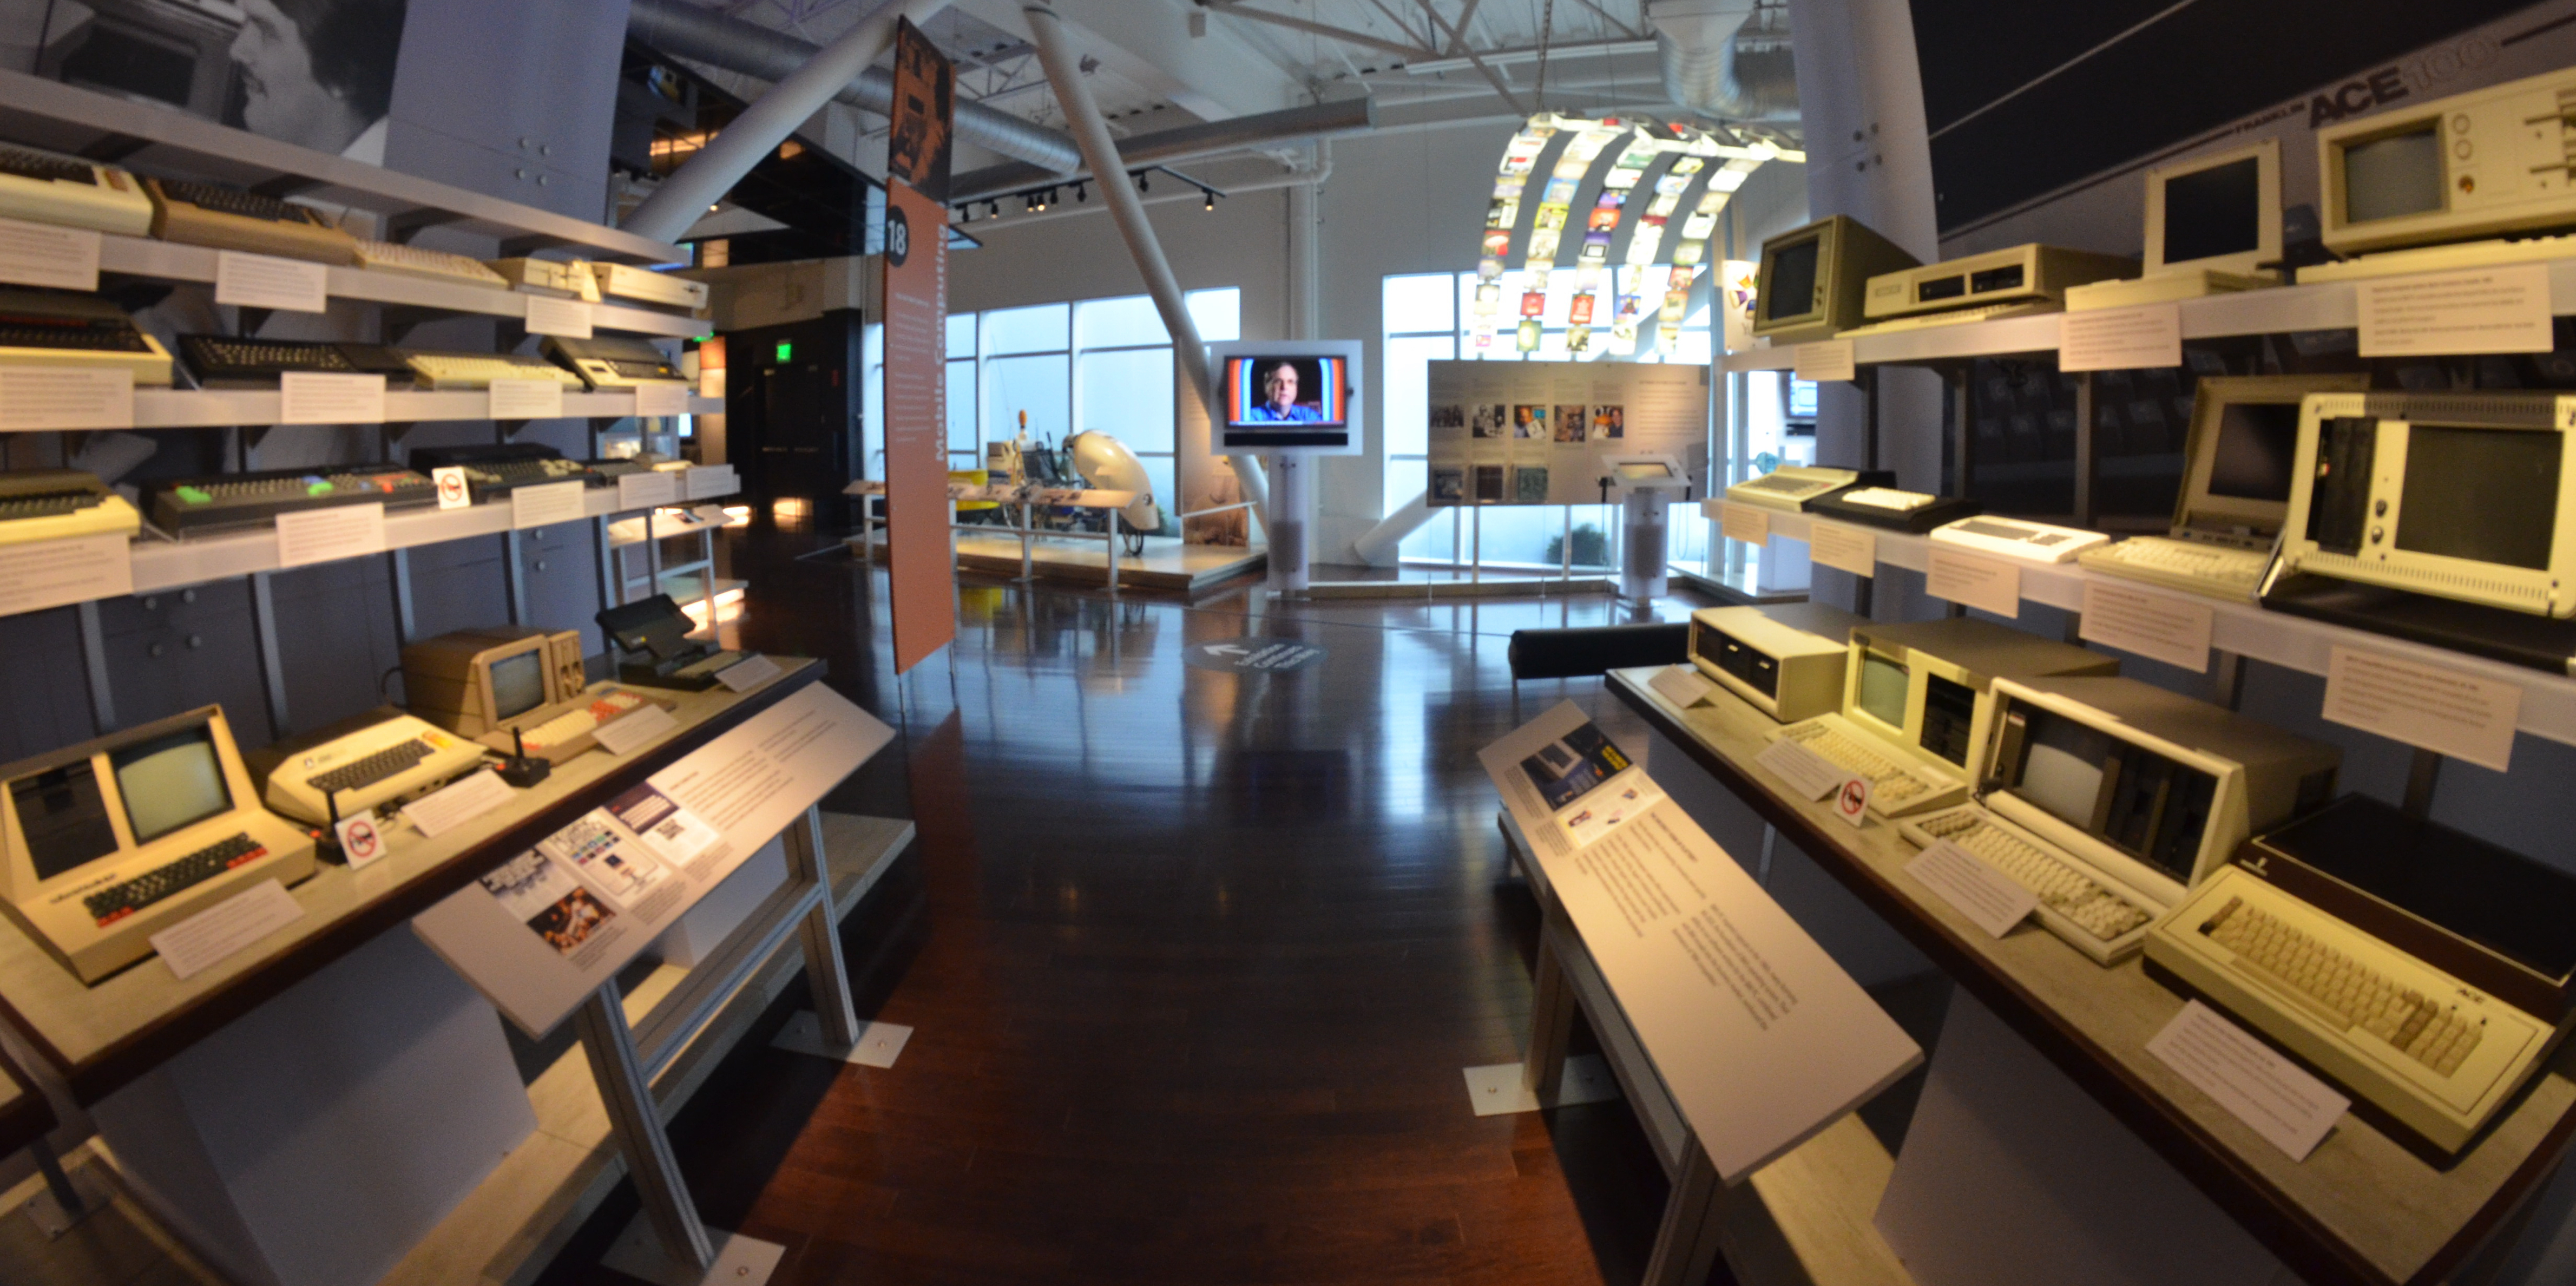
\includegraphics[width=\paperwidth]{cover}};
    \draw (current page.center) node [fill=primary, text=white, text opacity=1,inner sep=1cm]{\centering\bfseries\sffamily\parbox[c][][t]{\paperwidth}{\centering
    {\Large \@institution}\\[3pt] % Institution
    {\Huge \@title}\\[25pt] % Book title
    {\huge \@subtitle}\\[15pt] % Subtitle
    {\Large por \@author}\\[20pt] % Author
    {\large Ver. \@version \quad (\@date)}}}; % Version and date
    \end{tikzpicture}
    \vfill
    \endgroup
}
\makeatother

% Part text styling
\titlecontents{part}[0cm]
{\addvspace{20pt}\centering\large\bfseries}
{}
{}
{}

% Chapter text styling
\titlecontents{chapter}[1.25cm] % Indentation
{\addvspace{12pt}\large\sffamily\bfseries} % Spacing and font options for chapters
{\color{primary!60}\contentslabel[\Large\thecontentslabel]{1.25cm}\color{primary}} % Chapter number
{\color{primary}}
{\color{primary!60}\normalsize\;\titlerule*[.5pc]{.}\;\thecontentspage} % Page number

% Section text styling
\titlecontents{section}[1.25cm] % Indentation
{\addvspace{3pt}\sffamily\bfseries} % Spacing and font options for sections
{\contentslabel[\thecontentslabel]{1.25cm}} % Section number
{}
{\hfill\color{black}\thecontentspage} % Page number
[]

% Subsection text styling
\titlecontents{subsection}[1.25cm] % Indentation
{\addvspace{1pt}\sffamily\small} % Spacing and font options for subsections
{\contentslabel[\thecontentslabel]{1.25cm}} % Subsection number
{}
{\ \titlerule*[.5pc]{.}\;\thecontentspage} % Page number
[]

% List of figures
\titlecontents{figure}[0em]
{\addvspace{-5pt}\sffamily}
{\thecontentslabel\hspace*{1em}}
{}
{\ \titlerule*[.5pc]{.}\;\thecontentspage}
[]

% List of tables
\titlecontents{table}[0em]
{\addvspace{-5pt}\sffamily}
{\thecontentslabel\hspace*{1em}}
{}
{\ \titlerule*[.5pc]{.}\;\thecontentspage}
[]

%----------------------------------------------------------------------------------------
%	MINI TABLE OF CONTENTS IN PART HEADS
%----------------------------------------------------------------------------------------

% Chapter text styling
\titlecontents{lchapter}[0em] % Indenting
{\addvspace{15pt}\large\sffamily\bfseries} % Spacing and font options for chapters
{\color{primary}\contentslabel[\Large\thecontentslabel]{1.25cm}\color{primary}} % Chapter number
{}
{\color{primary}\normalsize\sffamily\bfseries\;\titlerule*[.5pc]{.}\;\thecontentspage} % Page number

% Section text styling
\titlecontents{lsection}[0em] % Indenting
{\sffamily\small} % Spacing and font options for sections
{\contentslabel[\thecontentslabel]{1.25cm}} % Section number
{}
{}

% Subsection text styling
\titlecontents{lsubsection}[.5em] % Indentation
{\normalfont\footnotesize\sffamily} % Font settings
{}
{}
{}

%----------------------------------------------------------------------------------------
%	PAGE HEADERS
%----------------------------------------------------------------------------------------

\usepackage{fancyhdr} % Required for header and footer configuration

\pagestyle{fancy}
\renewcommand{\chaptermark}[1]{\markboth{\sffamily\normalsize\bfseries\chaptername\ \thechapter.\ #1}{}} % Chapter text font settings
\renewcommand{\sectionmark}[1]{\markright{\sffamily\normalsize\thesection\hspace{5pt}#1}{}} % Section text font settings
\fancyhf{} \fancyhead[LE,RO]{\sffamily\normalsize\thepage} % Font setting for the page number in the header
\fancyhead[LO]{\rightmark} % Print the nearest section name on the left side of odd pages
\fancyhead[RE]{\leftmark} % Print the current chapter name on the right side of even pages
\renewcommand{\headrulewidth}{0.5pt} % Width of the rule under the header
\addtolength{\headheight}{2.5pt} % Increase the spacing around the header slightly
\renewcommand{\footrulewidth}{0pt} % Removes the rule in the footer
\fancypagestyle{plain}{\fancyhead{}\renewcommand{\headrulewidth}{0pt}} % Style for when a plain pagestyle is specified

% Removes the header from odd empty pages at the end of chapters
\makeatletter
\renewcommand{\cleardoublepage}{
\clearpage\ifodd\c@page\else
\hbox{}
\vspace*{\fill}
\thispagestyle{empty}
\newpage
\fi}

%----------------------------------------------------------------------------------------
%	THEOREM STYLES
%----------------------------------------------------------------------------------------

\usepackage{amsmath,amsfonts,amssymb,amsthm} % For math equations, theorems, symbols, etc

\newcommand{\intoo}[2]{\mathopen{]}#1\,;#2\mathclose{[}}
\newcommand{\ud}{\mathop{\mathrm{{}d}}\mathopen{}}
\newcommand{\intff}[2]{\mathopen{[}#1\,;#2\mathclose{]}}
\newtheorem{notation}{Notación}[chapter]

% Boxed/framed environments
\newtheoremstyle{primarynumbox}% % Theorem style name
{0pt}% Space above
{0pt}% Space below
{\normalfont}% % Body font
{}% Indent amount
{\small\bf\sffamily\color{primary}}% % Theorem head font
{\;}% Punctuation after theorem head
{0.25em}% Space after theorem head
{\small\sffamily\color{primary}\thmname{#1}\nobreakspace\thmnumber{\@ifnotempty{#1}{}\@upn{#2}}% Theorem text (e.g. Theorem 2.1)
\thmnote{\nobreakspace\the\thm@notefont\sffamily\bfseries\color{black}---\nobreakspace#3.}} % Optional theorem note
\renewcommand{\qedsymbol}{$\blacksquare$}% Optional qed square

\newtheoremstyle{blacknumex}% Theorem style name
{5pt}% Space above
{5pt}% Space below
{\normalfont}% Body font
{} % Indent amount
{\small\bf\sffamily}% Theorem head font
{\;}% Punctuation after theorem head
{0.25em}% Space after theorem head
{\small\sffamily{\tiny\ensuremath{\textcolor{primary}{\blacksquare}}}\nobreakspace\thmname{#1}\nobreakspace\thmnumber{\@ifnotempty{#1}{}\@upn{#2}}\\% Theorem text (e.g. Theorem 2.1)
\thmnote{\nobreakspace\the\thm@notefont\sffamily\bfseries---\nobreakspace#3.}}% Optional theorem note

\newtheoremstyle{blacknumbox} % Theorem style name
{0pt}% Space above
{0pt}% Space below
{\normalfont}% Body font
{}% Indent amount
{\small\bf\sffamily}% Theorem head font
{\;}% Punctuation after theorem head
{0.25em}% Space after theorem head
{\small\sffamily\thmname{#1}\nobreakspace\thmnumber{\@ifnotempty{#1}{}\@upn{#2}}% Theorem text (e.g. Theorem 2.1)
\thmnote{\nobreakspace\the\thm@notefont\sffamily\bfseries---\nobreakspace#3.}}% Optional theorem note

% Non-boxed/non-framed environments
\newtheoremstyle{primarynum}% % Theorem style name
{5pt}% Space above
{5pt}% Space below
{\normalfont}% % Body font
{}% Indent amount
{\small\bf\sffamily\color{primary}}% % Theorem head font
{\;}% Punctuation after theorem head
{0.25em}% Space after theorem head
{\small\sffamily\color{primary}\thmname{#1}\nobreakspace\thmnumber{\@ifnotempty{#1}{}\@upn{#2}}% Theorem text (e.g. Theorem 2.1)
\thmnote{\nobreakspace\the\thm@notefont\sffamily\bfseries\color{black}---\nobreakspace#3.}} % Optional theorem note
\renewcommand{\qedsymbol}{$\blacksquare$}% Optional qed square
\makeatother

% Defines the theorem text style for each type of theorem to one of the three styles above
\newcounter{dummy}
\numberwithin{dummy}{section}
\theoremstyle{primarynumbox}
\newtheorem{theoremeT}[dummy]{Teorema}
\newtheorem{problem}{Problema}[chapter]
\newtheorem{exerciseT}{Ejercicio}[chapter]
\theoremstyle{blacknumex}
\newtheorem{exampleT}{Ejemplo}[chapter]
\theoremstyle{blacknumbox}
\newtheorem{vocabulary}{Vocabulario}[chapter]
\newtheorem{definitionT}{Definición}[chapter]
\newtheorem{corollaryT}[dummy]{Corolario}
\theoremstyle{primarynum}
\newtheorem{proposition}[dummy]{Proposición}

%----------------------------------------------------------------------------------------
%	DEFINITION OF COLORED BOXES
%----------------------------------------------------------------------------------------

\RequirePackage[framemethod=default]{mdframed} % Required for creating the theorem, definition, exercise and corollary boxes

% Theorem box
\newmdenv[skipabove=7pt,
skipbelow=7pt,
backgroundcolor=black!5,
linecolor=primary,
innerleftmargin=5pt,
innerrightmargin=5pt,
innertopmargin=5pt,
leftmargin=0cm,
rightmargin=0cm,
innerbottommargin=5pt]{tBox}

% Exercise box
\newmdenv[skipabove=5pt,
skipbelow=7pt,
rightline=false,
leftline=true,
topline=false,
bottomline=false,
backgroundcolor=primary!10,
linecolor=primary,
innerleftmargin=5pt,
innerrightmargin=5pt,
innertopmargin=10pt,
innerbottommargin=5pt,
leftmargin=0cm,
rightmargin=0cm,
linewidth=4pt]{eBox}

% Definition box
\newmdenv[skipabove=17pt,
skipbelow=7pt,
rightline=false,
leftline=true,
topline=false,
bottomline=false,
linecolor=primary,
innerleftmargin=5pt,
innerrightmargin=5pt,
innertopmargin=10pt,
innerbottommargin=5pt,
leftmargin=0cm,
rightmargin=0cm,
linewidth=4pt]{dBox}

% Corollary box
\newmdenv[skipabove=7pt,
skipbelow=7pt,
rightline=false,
leftline=true,
topline=false,
bottomline=false,
linecolor=gray,
backgroundcolor=black!5,
innerleftmargin=5pt,
innerrightmargin=5pt,
innertopmargin=5pt,
leftmargin=0cm,
rightmargin=0cm,
linewidth=4pt,
innerbottommargin=5pt]{cBox}

% Creates an environment for each type of theorem and assigns it a theorem text style from the "Theorem Styles" section above and a colored box from above
\newenvironment{theorem}{\begin{tBox}\begin{theoremeT}}{\end{theoremeT}\end{tBox}}
\newenvironment{exercise}{\begin{eBox}\begin{exerciseT}}{\hfill{\color{primary}\tiny\ensuremath{\blacksquare}}\end{exerciseT}\end{eBox}}
\newenvironment{knowwhat}[1][Sabías qué]{\begin{eBox}\textcolor{primary}{\textbf{#1}}\\}{\hfill{\color{primary}}\end{eBox}}
\newenvironment{definition}{\begin{dBox}\begin{definitionT}}{\end{definitionT}\end{dBox}}
\newenvironment{example}{\begin{exampleT}}{\hfill{\tiny\ensuremath{\blacksquare}}\end{exampleT}}
\newenvironment{corollary}{\begin{cBox}\begin{corollaryT}}{\end{corollaryT}\end{cBox}}
\newenvironment{solution}{\vspace*{10pt}}{\vspace*{30pt}}

%----------------------------------------------------------------------------------------
%	REMARK ENVIRONMENT
%----------------------------------------------------------------------------------------

\newenvironment{remark}{\par\vspace{10pt}\small % Vertical white space above the remark and smaller font size
\begin{list}{}{
\leftmargin=35pt % Indentation on the left
\rightmargin=25pt}\item\ignorespaces % Indentation on the right
\makebox[-2.5pt]{\begin{tikzpicture}[overlay]
\node[draw=primary!60,line width=1pt,circle,fill=primary!25,font=\sffamily\bfseries,inner sep=2pt,outer sep=0pt] at (-15pt,0pt){\textcolor{primary}{!}};\end{tikzpicture}} % Orange R in a circle
\advance\baselineskip -1pt}{\end{list}\vskip5pt} % Tighter line spacing and white space after remark

\newenvironment{hint}{\par\vspace{10pt}\small % Vertical white space above the remark and smaller font size
\begin{list}{}{
\leftmargin=35pt % Indentation on the left
\rightmargin=25pt}\item\ignorespaces % Indentation on the right
\makebox[-2.5pt]{\begin{tikzpicture}[overlay]
\node[draw=yellow!60,line width=1pt,circle,fill=yellow!25,font=\sffamily\bfseries,inner sep=2pt,outer sep=0pt] at (-15pt,0pt){\textcolor{yellow}{X}};\end{tikzpicture}} % Orange R in a circle
\advance\baselineskip -1pt}{\end{list}\vskip5pt} % Tighter line spacing and white space after remark

\newenvironment{question}{\par\vspace{10pt}\small % Vertical white space above the remark and smaller font size
\begin{list}{}{
\leftmargin=35pt % Indentation on the left
\rightmargin=25pt}\item\ignorespaces % Indentation on the right
\makebox[-2.5pt]{\begin{tikzpicture}[overlay]
\node[draw=blue!60,line width=1pt,circle,fill=blue!25,font=\sffamily\bfseries,inner sep=2pt,outer sep=0pt] at (-15pt,0pt){\textcolor{blue}{?}};\end{tikzpicture}} % Orange R in a circle
\advance\baselineskip -1pt}{\end{list}\vskip5pt} % Tighter line spacing and white space after remark

\newenvironment{money}{\par\vspace{10pt}\small % Vertical white space above the remark and smaller font size
\begin{list}{}{
\leftmargin=35pt % Indentation on the left
\rightmargin=25pt}\item\ignorespaces % Indentation on the right
\makebox[-2.5pt]{\begin{tikzpicture}[overlay]
\node[draw=green!60,line width=1pt,circle,fill=green!25,font=\sffamily\bfseries,inner sep=2pt,outer sep=0pt] at (-15pt,0pt){\textcolor{green}{\$}};\end{tikzpicture}} % Orange R in a circle
\advance\baselineskip -1pt}{\end{list}\vskip5pt} % Tighter line spacing and white space after remark


%----------------------------------------------------------------------------------------
%	SECTION NUMBERING IN THE MARGIN
%----------------------------------------------------------------------------------------

\makeatletter
\renewcommand{\@seccntformat}[1]{\llap{\textcolor{primary}{\csname the#1\endcsname}\hspace{1em}}}
\renewcommand{\section}{\@startsection{section}{1}{\z@}
{-4ex \@plus -1ex \@minus -.4ex}
{1ex \@plus.2ex }
{\normalfont\large\sffamily\bfseries}}
\renewcommand{\subsection}{\@startsection {subsection}{2}{\z@}
{-3ex \@plus -0.1ex \@minus -.4ex}
{0.5ex \@plus.2ex }
{\normalfont\sffamily\bfseries}}
\renewcommand{\subsubsection}{\@startsection {subsubsection}{3}{\z@}
{-2ex \@plus -0.1ex \@minus -.2ex}
{.2ex \@plus.2ex }
{\normalfont\small\sffamily\bfseries}}
\renewcommand\paragraph{\@startsection{paragraph}{4}{\z@}
{-2ex \@plus-.2ex \@minus .2ex}
{.1ex}
{\normalfont\small\sffamily\bfseries}}

%----------------------------------------------------------------------------------------
%	PART HEADINGS
%----------------------------------------------------------------------------------------

% numbered part in the table of contents
\newcommand{\@mypartnumtocformat}[2]{%
\setlength\fboxsep{0pt}%
\noindent\colorbox{primary!20}{\strut\parbox[c][.7cm]{\ecart}{\color{primary!70}\Large\sffamily\bfseries\centering#1}}\hskip\esp\colorbox{primary!40}{\strut\parbox[c][.7cm]{\linewidth-\ecart-\esp}{\Large\sffamily\centering#2}}}%
%%%%%%%%%%%%%%%%%%%%%%%%%%%%%%%%%%
% unnumbered part in the table of contents
\newcommand{\@myparttocformat}[1]{%
\setlength\fboxsep{0pt}%
\noindent\colorbox{primary!40}{\strut\parbox[c][.7cm]{\linewidth}{\Large\sffamily\centering#1}}}%
%%%%%%%%%%%%%%%%%%%%%%%%%%%%%%%%%%
\newlength\esp
\setlength\esp{4pt}
\newlength\ecart
\setlength\ecart{1.2cm-\esp}
\newcommand{\thepartimage}{}%
\newcommand{\partimage}[1]{\renewcommand{\thepartimage}{#1}}%
\def\@part[#1]#2{%
\ifnum \c@secnumdepth >-2\relax%
\refstepcounter{part}%
\addcontentsline{toc}{part}{\texorpdfstring{\protect\@mypartnumtocformat{\thepart}{#1}}{\partname~\thepart\ ---\ #1}}
\else%
\addcontentsline{toc}{part}{\texorpdfstring{\protect\@myparttocformat{#1}}{#1}}%
\fi%
\startcontents%
\markboth{}{}%
{\thispagestyle{empty}%
\begin{tikzpicture}[remember picture,overlay]%
\node at (current page.north west){\begin{tikzpicture}[remember picture,overlay]%
\fill[primary!20](0cm,0cm) rectangle (\paperwidth,-\paperheight);
\node[anchor=north] at (4cm,-3.25cm){\color{primary!40}\fontsize{220}{100}\sffamily\bfseries\thepart};
\node[anchor=south east] at (\paperwidth-1cm,-\paperheight+1cm){\parbox[t][][t]{8.5cm}{
\printcontents{l}{0}{\setcounter{tocdepth}{1}}%
}};
\node[anchor=north east] at (\paperwidth-1.5cm,-3.25cm){\parbox[t][][t]{15cm}{\strut\raggedleft\color{white}\fontsize{30}{30}\sffamily\bfseries#2}};
\end{tikzpicture}};
\end{tikzpicture}}%
\@endpart}
\def\@spart#1{%
\startcontents%
\phantomsection
{\thispagestyle{empty}%
\begin{tikzpicture}[remember picture,overlay]%
\node at (current page.north west){\begin{tikzpicture}[remember picture,overlay]%
\fill[primary!20](0cm,0cm) rectangle (\paperwidth,-\paperheight);
\node[anchor=north east] at (\paperwidth-1.5cm,-3.25cm){\parbox[t][][t]{15cm}{\strut\raggedleft\color{white}\fontsize{30}{30}\sffamily\bfseries#1}};
\end{tikzpicture}};
\end{tikzpicture}}
\addcontentsline{toc}{part}{\texorpdfstring{%
\setlength\fboxsep{0pt}%
\noindent\protect\colorbox{primary!40}{\strut\protect\parbox[c][.7cm]{\linewidth}{\Large\sffamily\protect\centering #1\quad\mbox{}}}}{#1}}%
\@endpart}
\def\@endpart{\vfil\newpage
\if@twoside
\if@openright
\null
\thispagestyle{empty}%
\newpage
\fi
\fi
\if@tempswa
\twocolumn
\fi}

%----------------------------------------------------------------------------------------
%	CHAPTER HEADINGS
%----------------------------------------------------------------------------------------

% A switch to conditionally include a picture, implemented by  Christian Hupfer
\newif\ifusechapterimage
\usechapterimagetrue
\newcommand{\thechapterimage}{}%
\newcommand{\thechapterimagedescription}{}%
\newcommand{\thechapterimageauthor}{}%
\newcommand{\chapterimage}[1]{\ifusechapterimage\renewcommand{\thechapterimage}{#1}\fi}%
\newcommand{\chapterimagedescription}[1]{\ifusechapterimage\renewcommand{\thechapterimagedescription}{#1}\fi}%
\newcommand{\chapterimageauthor}[1]{\ifusechapterimage\renewcommand{\thechapterimageauthor}{#1}\fi}%
\newcommand{\autodot}{.}
\def\@makechapterhead#1{%
{\parindent \z@ \raggedright \normalfont
\ifnum \c@secnumdepth >\m@ne
\if@mainmatter
\begin{tikzpicture}[remember picture,overlay]
\node at (current page.north west)
{\begin{tikzpicture}[remember picture,overlay]
\node[anchor=north west,inner sep=0pt] at (0,0) {\ifusechapterimage\includegraphics[width=\paperwidth]{\thechapterimage}\fi};
\draw[anchor=west] (\Gm@lmargin,-9cm) node [line width=2pt,rounded corners=15pt,draw=primary,fill=white,fill opacity=0.5,inner sep=15pt]{\strut\makebox[22cm]{}};
\draw[anchor=west] (\Gm@lmargin+.3cm,-9cm) node {\huge\sffamily\bfseries\color{black}\thechapter\autodot~#1\strut};
\draw[anchor=east] (\Gm@lmargin+17.5cm,-11.5cm) node {\ifusechapterimage{\raggedright\color{gray}\thechapterimagedescription\autodot}\fi};
\draw[anchor=east] (\Gm@lmargin+17.5cm,-12cm) node {\ifusechapterimage{\raggedright\color{gray}\thechapterimageauthor\autodot}\fi};
\end{tikzpicture}};
\end{tikzpicture}
\else
\begin{tikzpicture}[remember picture,overlay]
\node at (current page.north west)
{\begin{tikzpicture}[remember picture,overlay]
\node[anchor=north west,inner sep=0pt] at (0,0) {\ifusechapterimage\includegraphics[width=\paperwidth]{\thechapterimage}\fi};
\draw[anchor=west] (\Gm@lmargin,-9cm) node [line width=2pt,rounded corners=15pt,draw=primary,fill=white,fill opacity=0.5,inner sep=15pt]{\strut\makebox[22cm]{}};
\draw[anchor=west] (\Gm@lmargin+.3cm,-9cm) node {\huge\sffamily\bfseries\color{black}#1\strut};
%\draw[anchor=east] (\Gm@lmargin+17.5cm,-11cm) node {\ifusechapterimage{\raggedright\color{gray}\thechapterimagedescription\autodot}\fi};
%\draw[anchor=east] (\Gm@lmargin+17.5cm,-11.5cm) node {\ifusechapterimage{\raggedright\color{gray}\thechapterimageauthor\autodot}\fi};
\end{tikzpicture}};
\end{tikzpicture}
\fi\fi\par\vspace*{270\p@}}}

%-------------------------------------------

\def\@makeschapterhead#1{%
\begin{tikzpicture}[remember picture,overlay]
\node at (current page.north west)
{\begin{tikzpicture}[remember picture,overlay]
\node[anchor=north west,inner sep=0pt] at (0,0) {\ifusechapterimage\includegraphics[width=\paperwidth]{\thechapterimage}\fi};
\draw[anchor=west] (\Gm@lmargin,-9cm) node [line width=2pt,rounded corners=15pt,draw=primary,fill=white,fill opacity=0.5,inner sep=15pt]{\strut\makebox[22cm]{}};
\draw[anchor=west] (\Gm@lmargin+.3cm,-9cm) node {\huge\sffamily\bfseries\color{black}#1\strut};
\draw[anchor=east] (\Gm@lmargin+17.5cm,-11.5cm) node {\ifusechapterimage{\raggedright\color{gray}\thechapterimagedescription\autodot}\fi};
\draw[anchor=east] (\Gm@lmargin+17.5cm,-12cm) node {\ifusechapterimage{\raggedright\color{gray}\thechapterimageauthor\autodot}\fi};
\end{tikzpicture}};
\end{tikzpicture}
\par\vspace*{270\p@}}
\makeatother

%----------------------------------------------------------------------------------------
%	HYPERLINKS IN THE DOCUMENTS
%----------------------------------------------------------------------------------------

\usepackage{hyperref}
\hypersetup{hidelinks,backref=true,pagebackref=true,hyperindex=true,colorlinks=false,breaklinks=true,urlcolor= primary,bookmarks=true,bookmarksopen=false,pdftitle={Title},pdfauthor={Author}}
\usepackage{bookmark}
\bookmarksetup{
open,
numbered,
addtohook={%
\ifnum\bookmarkget{level}=0 % chapter
\bookmarksetup{bold}%
\fi
\ifnum\bookmarkget{level}=-1 % part
\bookmarksetup{color=primary,bold}%
\fi
}
}

%----------------------------------------------------------------------------------------
%	SPECIAL TRANSLATIONS
%----------------------------------------------------------------------------------------
\addto\extrasspanish{%
\def\partautorefname{Unidad}%
\def\appendixautorefname{Anexo}%
}

%----------------------------------------------------------------------------------------
%	SPECIAL INDENTS AND LINES
%----------------------------------------------------------------------------------------
\newcommand{\crline}[2][10pt]{
    \noindent #2

    \vspace{#1}
}

\newcounter{sindentwidth}
\newcounter{dindentwidth}
\setcounter{sindentwidth}{16}
\setcounter{dindentwidth}{32}

\newcommand{\sindent}{\noindent\hspace*{\value{sindentwidth} pt}}
\newcommand{\dindent}{\noindent\hspace*{\value{dindentwidth} pt}}

%----------------------------------------------------------------------------------------
%	EMOJI IMAGES SUPPORT (IMAGES NOT PROVIDED)
%----------------------------------------------------------------------------------------
\newcommand{\emoji}[1]{%
  \includegraphics[width=1em,valign=t,raise=-0.1em]{#1}%
}

%----------------------------------------------------------------------------------------
%	DARK MODE SUPPORT
%----------------------------------------------------------------------------------------
\newcommand{\darkmode}{
  \pagecolor{black!80}
  \color{white!30}
}
 % Insert the thebook.tex file which contains the majority of the structure behind the template

\usepackage{colortbl} % For logic tables coloring

% Some additional greek leters
\newcommand{\Alpha}{A}%
\newcommand{\Beta}{B}%
\newcommand{\Epsilon}{E}%
\newcommand{\Zeta}{Z}%
\newcommand{\Eta}{H}%
\newcommand{\Iota}{I}%
\newcommand{\Kappa}{K}%
\newcommand{\Mu}{M}%
\newcommand{\Nu}{N}%
\newcommand{\omicrom}{o}%
\newcommand{\Omicrom}{O}%
\newcommand{\Rho}{P}%
\newcommand{\Tau}{T}%
\newcommand{\Chi}{X}%

% \lnot, \land and \lor are already available in LaTeX
% \rowcolor{gray}
\newcommand{\lxor}{\veebar}%
\newcommand{\lthen}{\to}%
\newcommand{\liff}{\leftrightarrow}%
\newcommand{\lseq}{\vdash}%
\newcommand{\ltrue}{{\color{ForestGreen}V}}%
\newcommand{\lfalse}{{\color{BrickRed}{F}}}%
\newcommand{\ltruefull}{{\color{ForestGreen}VERDADERO}}%
\newcommand{\lfalsefull}{{\color{BrickRed}FALSO}}%

\makeatletter
\define@cmdkey[]{lreasoning}{width}[1\textwidth]{}
\define@cmdkey[]{lreasoning}{dividerheight}[2pt]{}
\define@cmdkey[]{lreasoning}{margin}[0pt]{}
\setkeys[]{lreasoning}{width=1\textwidth,dividerheight=2pt,margin=0pt}

\newenvironment{lreasoning}[1][width=1\textwidth,dividerheight=3pt,margin=0pt]{
  \setkeys[]{lreasoning}{#1}
  \begin{minipage}[t]{\cmdlreasoning@width}
}{
  \end{minipage}
}%
\newcommand{\lreasonrule}[0]{%
  \parbox[c][\cmdlreasoning@dividerheight][c]{1\textwidth}{\noindent\hspace*{\cmdlreasoning@margin}\hrulefill}\\%
}%
\newcommand{\lpremise}[1]{%
  \noindent\hspace*{\cmdlreasoning@margin}#1\\%
}%
\newcommand{\lconclusion}[1]{%
  \lreasonrule%
  \noindent\hspace*{\cmdlreasoning@margin}#1%
}%
\makeatother % Add definition for logic elements

\addbibresource{bibliography.bib}

% \darkmode

\begin{document}

%----------------------------------------------------------------------------------------
%	DOCUMENT CONFIGURATION
%----------------------------------------------------------------------------------------

\title{Elementos de Programación y Lógica}
\subtitle{Solucionario del Cuadernillo del Estudiante}
\department{Departamento de Ciencia y Tecnología}
\institution{Universidad Nacional de Quilmes}
\author{Alan Rodas Bonjour}
\version{0.6.0}
\date{24/04/2022}

\primarycolor{176}{30}{45}

\maketitle

\newpage
~\vfill
\thispagestyle{empty}

\crline{Copyright \copyright\ 2019 Alan Rodas Bonjour} % Copyright notice

\crline{\textsc{Publicado online por Alan Rodas Bonjour}} % Publisher

\crline[25pt]{\textsc{http://elementosdeprogramacionylogica.web.unq.edu.ar}} % URL


\crline{\includegraphics[scale=0.5]{cc-by-nc-sa}}

\crline{Licenciado bajo los términos de la siguiente licencia de contenidos:
Licencia Creative Commons Atribución-NoComercial-CompartirIgual 4.0 Internacional
(la ``licencia''). Puede obtener una copia completa de ella en
\url{https://creativecommons.org/licenses/by-nc-sa/4.0/deed.es}.}

\crline{
    Usted tiene derecho a:
    \begin{itemize}
        \item \textbf{Compartir}: copiar y redistribuir el material en cualquier
        medio o formato
        \item \textbf{Adaptar}: remezclar, transformar y construir a partir del
        material
    \end{itemize}
}

\crline{El licenciante no puede revocar estas libertades en tanto usted siga los
términos siguientes.}

\crline{
    \begin{itemize}
        \item \textbf{Atribución}: Usted debe dar crédito de manera adecuada,
        brindar un enlace a la licencia, e indicar si se han realizado cambios.
        Puede hacerlo en cualquier forma razonable, pero no de forma tal que
        sugiera que usted o su uso tienen el apoyo de la licenciante.
        \item \textbf{NoComercial}: Usted no puede hacer uso del material con
        propósitos comerciales.
        \item \textbf{CompartirIgual}: Si remezcla, transforma o crea a partir
        del material, debe distribuir su contribución bajo la la misma licencia
        del original.
    \end{itemize}
}

\crline{No hay restricciones adicionales — No puede aplicar términos legales ni
medidas tecnológicas que restrinjan legalmente a otras a hacer cualquier uso
permitido por la licencia.}

\crline{No tiene que cumplir con la licencia para elementos del material en el
dominio público o cuando su uso esté permitido por una excepción o limitación
aplicable.}

\crline{No se dan garantías. La licencia podría no darle todos los permisos que
 necesita para el uso que tenga previsto. Por ejemplo, otros derechos como
 publicidad, privacidad, o derechos morales pueden limitar la forma en que
 utilice el material.}

% License information

\crline{\textit{Primera edición, Febrero 2019}} % Printing/edition date


\chapterimage{indice}
\pagestyle{empty}
\tableofcontents
\cleardoublepage
\pagestyle{fancy}

\setlength{\parskip}{0.5em}

%\input{introduccion_solucionario}
\part{Computadoras}
\label{unit:computadoras}

\chapterimage{unidades/1_computadoras/1_computadoras/imagenes/cover}
\chapterimagedescription{Placa base de una computadora con sus circuitos impresos}
\chapterimageauthor{Fotografía de Blickpixel}

\chapter{Computadoras}

\setcounter{section}{2}
\section{Actividades}
\index{Actividades}

Responda las siguientes preguntas. Puede investigar en Internet si lo cree
conveniente.

\begin{exercise}
Mire el cartel a continuación\\
\includegraphics[scale=0.38]{unidades/1_computadoras/1_computadoras/imagenes/iphone_x_specs.png}

Determine.\\
¿Cuáles de los elementos mencionados corresponden a software?\\
¿Cuáles de los elementos mencionados corresponden a hardware?
\end{exercise}

En el cartel, los siguientes elementos aluden directamente al software:

\begin{itemize}
    \item Filtros y colores en Photos
    \item FaceID para reconocimiento facial
    \item iOS 11 con Siri
    \item Llamadas de video con FaceTime
\end{itemize}

Mientras que los siguientes elementos aluden al hardware:

\begin{itemize}
    \item Chip A11 Bionics de 64 bits
    \item Pantalla OLED multitouch de 5.8"
    \item Cámaras de 12MP con gran angular y teleobjetivo
    \item WiFi 802.11ac con MIMO
    \item Bluetooth 5.0
    \item NFC con modo lectura
    \item Bocina estéreo integrada y micrófono de alta calidad
    \item Hasta 21hs de batería en conversación
\end{itemize}

Cada uno de los elementos de hardware requiere de software para funcionar. Por
lo tanto, incluso si refieren a hardware, siempre hay software involucrado para
que el dispositivo funcione y se integre con el sistema operativo. El software
no necesariamente es una aplicación que viene por separado, sino que son partes
especificas del sistema operativo que dar soporte a ese hardware, lo cual se
realiza en forma de firmware, drivers u otros.
\vspace{1cm}

\begin{exercise}
¿Qué sistemas operativos conoce?\\
Discuta su respuesta con compañeros y el docente para descubrir nuevos sistemas.
\end{exercise}


Existen muchos sistemas operativos, algunos ya mencionados en el libro.
Repasemos algunos de ellos, e indagemos sobre otros:

\subsection*{Microsoft Windows}

El más conocido es tal vez \textbf{Microsoft Windows}, debido a que es el
sistema que viene instalado por defecto en muchas computadoras.
\textbf{Microsoft} hizo un acuerdo con la empresa \textbf{IBM}, en donde sus
máquinas se vendían con Windows pre-instalado en sus equipos, que en los 80s y
principios de los 90s eran el estándar de la industria. A medida que aparecían
otros jugadores en la industria del hardware, Microsoft establecía contratos
draconianos para que Windows fuera el sistema por defecto en sus equipos, a la
vez que las empresas de hardware buscaban estos contratos en pos de captar
usuarios ya fieles al sistema operativo de las ventanas.

Microsoft establecería una fuerte campaña de eliminación de la competencia y
monopolio del mercado, al iniciar acuerdos con diversas dependencias del Estado
en las que entregaban Windows de forma gratuita (solo inicialmente), por ejemplo
en el área de educación.

Esto hizo que muchas personas solo hayan sido expuestas a este sistema
operativo, y por tanto es el único que conocen. Peor aún, es el único que saben
manejar, y por tanto, cuando necesitan una nueva computadora, esta debe venir
con Windows (el usuario debe pagar un adicional) o debe instalarse luego (se
debe comprar la licencia).

\image{soluciones/1_computadoras/1_computadoras/imagenes/bliss.jpg}
{Bliss, la imágen de fondo por defecto de Windows XP se ha transformado en un
ícono de ese sistema.} {Imágen de Azuresh.}

Las primeras versiones de Windows estaban basadas en \textbf{MS-DOS}, otro
popular sistema de Microsoft de los 80s. Tuvo varias versiones a lo largo de su
historia, como \textbf{Windows 1.0}, \textbf{Windows 2.0} y \textbf{Windows 3.1}
(Las primeras versiones bastante primitivas, pero que sentaron las bases para
las demás, y donde se desarrolla el concepto de ventana), \textbf{Windows 95}
(El primero en tener el ``botón de inicio''), \textbf{Windows 98} (primero con
soporte para acceso a Internet por defecto), \textbf{Windows NT} (para
computadoras de uso empresarial), \textbf{Windows XP} (el primero en mezclar
tecnologías de NT, con las de 98, que hasta el momento eran tecnologías
separadas. Fue tal vez de las versiones más populares, saliendo en el año 2000),
\textbf{Windows 8} (donde se introdujo la interfaz Metro) y \textbf{Windows 10}
(la versión actual, que mezcla la interfaz Metro con una más tradicional).

\subsection*{MacOS}

Históricamente \textbf{Apple} ha desarrollado sus propios sistemas operativos,
para sus equipos (Ellos se definen como una empresa que vende computadoras, no
sistemas). Las primeras computadoras Apple, como la \textbf{Apple II}, venían
con \textbf{Apple DOS} y luego \textbf{Apple ProDOS}. Más tarde lanzaría lo que
posteriormente se conocería como \textbf{Mac OS}, en ese momento denominado
simplemente \textbf{System}, acompañando su nueva línea de computadoras
Macintosh.

Llegando el 2000, su sistema empezaría a sentir el paso de los años, un nuevo
sistema diseñado desde cero sería lanzado con toda su nueva línea de
computadoras, \textbf{Mac OS X}, sistema que hoy a recibido un rebranding, para
denominarse simplemente \textbf{macOS}, y que acompaña a todas las computadoras
de la marca.

A diferencia de otros sistemas operativos, macOS es un sistema que viene
instalado por defecto en los equipos de Apple, y que no se encuentra disponible
para otros equipos, ni siquiera como compra por separado.


\subsection*{GNU/Linux}

Cuándo inició el movimiento de \textbf{software libre} en 1984, \textbf{Richard
Stallman}, el fundador del movimiento, se propuso realizar un sistema operativo
completamente libre, compatible con \textbf{UNIX} (Un popular sistema de la
época, que era propiedad de AT\&T). Así, Stallman funda el \textbf{Proyecto
GNU}, bajo cuya ala aparecen cientos de herramientas necesarias para el
funcionamiento de un sistema operativo realmente utilizable, como compiladores,
editores, terminales, etc. Sin embargo, el proyecto \textbf{Hurd}, un
sub-proyecto de GNU que desarrollaría el \textbf{núcleo} del sistema operativo,
seguía teniendo cientos de retrasos, idas y vueltas, sin nunca terminar con una
versión utilizable. Ya en 1991, \textbf{Linus Torvalds}, un estudiante de la
Universidad de Helsinki en Finlandia, quería utilizar en su computadora hogareña
un sistema compatible con UNIX. Ante la ausencia de alternativas, se dispuso a
programar su propio sistema, y tras anunciar públicamente en un foro sobre su
desarrollo, Stallman se le acercó para convencerlo de que \textbf{Linux}, nombre
que recibiría el sistema operativo, debía ser libre.

Linux evolucionó, y al ser libre, miles de personas pueden contribuir al
proyecto. Su código es la base para múltiples sistemas operativos empaquetados
para el usuario final, que utilizan el núcleo Linux, junto con las herramientas
de GNU, y otros conjuntos de herramientas, imágenes, iconos, etc. (Lo que se
conoce como una \textbf{distribución}). Hay miles de distribuciones, como
\textbf{Ubuntu}, \textbf{Mint}, \textbf{Fedora}, \textbf{Debian}, \textbf{Arch},
\textbf{Zorin}, \textbf{Huayra}, entre otros tantos. Cualquiera con los
conocimientos técnicos suficientes puede crearse su propia distribución. Lo más
interesante es que existen distintas distribuciones, que se enfocan en distintas
cosas. Así por ejemplo, hay distribuciones para computadoras de escritorios,
otras para teléfonos celulares, otras para grandes servidores, para routers,
para computadoras viejas, para consolas de videojuegos, etc.

\subsection*{BSD}

\image{soluciones/1_computadoras/1_computadoras/imagenes/freebsd.png}
{Imágen de inicio de FreeBSD, corriendo sobre QEMU.} {Imágen de Huihermit.}

Los sistemas \textbf{BSD} (\textbf{Berkley Software Distribution}) comprenden,
al igual que Linux, un núcleo, y varias distribuciones derivadas de dicho núcleo
(Aunque incluso hay núcleos distintos e incompatibles entre si). El sistema
surgió en la \textbf{Universidad de Berkley}, en donde \textbf{Bill Joy} compiló
un conjunto de programas creados en la universidad que corrían sobre la versión
6 de UNIX. Otros universidades que utilizaban UNIX, podían entonces instalar
dichos programas en sus computadoras. Los programas comenzaron a crecer y a
incluir cambios en el mismo sistema UNIX. Sin embargo, por ser solo
modificaciones a partes del sistema, aunque Berkley distribuía todo el sistema
UNIX modificado, AT\&T seguía siendo el dueño del sistema, y por tanto, quien
quisiera utilizarlo debía pagar a AT\&T.

Tras una disputa legal que tomaría años resolver, Berkley dejaría de distribuir
el software. Tras la resolución del conflicto en 1992, y tras quitar todo rastro
de código del sistema UNIX original, se liberaría \textbf{BSD 4.2}. Berkley
distribuye el sistema bajo una licencia llamada \textbf{Licencia BSD}, que
permite que cualquiera pueda tomar el código de BSD y utilizarlo para lo que
quiera, inclusive, en proyectos comerciales de código cerrado.

Hoy hay varias distribuciones BSD, como \textbf{FreeBSD}, \textbf{OpenBSD}, y
\textbf{NetBSD}, pero hay muchas otras a su vez derivadas de estas tres. No solo
eso sino que \textbf{parte del código de BSD se encuentra en Windows}, y
\textbf{es la base para macOS de Apple}.

\subsection*{iOS}

\textbf{iOS} es un sistema operativo creado por \textbf{Apple} para que corra de
forma exclusiva en el \textbf{iPhone} y luego en \textbf{iPad}. El sistema
utiliza una gran cantidad de código de BSD, y también de macOS.

Este sistema se crea pensando en la optimización de recursos y de batería, así
como en una interfaz que pueda ser utilizada de forma sencilla en un dispositivo
que no cuenta ni con teclado ni mouse.

\subsection*{Android}

\textbf{Android} es un sistema creado por \textbf{Google}, basándose en el
núcleo de \textbf{Linux} (Aunque el mismo está altamente modificado para
funcionar de forma óptima en dispositivos móviles y tablets). El sistema, al
estar basado en Linux es software libre, pero la mayoría de los fabricantes de
teléfonos que venden dispositivos con Linux agregan gran cantidad de
herramientas no libres sobre el sistema, comenzando por \textbf{Google}, que
incluye no solo \textbf{Play Store}, sino también aplicaciones como
\textbf{Gmail}, \textbf{Calendar}, etc.

\subsection*{Otros sistemas}

Estos no son los únicos sistemas operativos. Existen cientos, y siempre aparecen
nuevos (Aunque muchos son altamente experimentales, o son solo prototipos que
fracasan). Ejemplos interesantes son \textbf{ReactOS} (Un sistema libre que
intenta generar un sistema completamente compatible con Windows XP),
\textbf{Haiku} (Un sistema que intenta revivir BeOS, y ser compatible con este),
\textbf{MenuetOS} (Un sistema operativo que pesa solo 3.25MB) y \textbf{Plan9}
(Un sistema operativo experimental de Bell Labs).

A lo largo de la historia han habido varios otros sistemas que han ganados
varios adeptos, y cuyas ideas innovadoras en muchos casos fueron luego adoptadas
por los sistemas comerciales más grandes, como \textbf{Amiga OS}, \textbf{BeOS},
\textbf{Symbian}, entre otros.

Finalmente podemos mencionar que existen sistemas operativos mucho más oscuros,
experimentales y casi sin usuarios. Un caso muy interesante es el
\textbf{TempleOS}, un sistema operativo con contenidos bíblicos, creado por
Terry A. Davis, quien lo creó con la intensión de transformar al sistema
operativo en el tercer templo profetizado en la biblia. Davis comenzó a sufrir
una serie de epizodios esquizofrénicos y alusinaciones sobre invasiones
extraterrestres y conspiraciones gubernamentales, motivo por el cual estuvo
hospitalizado en reiteradas ocasiones. Tras una autoproclamada ``revelación''
hacia su persona por Diós, con quien él dice tener comunicación directa, comenzó
el trabajo de desarrollar dicho sistema operativo, pues consideraba a otros
sistemas como impuros y llenos de pecado. TempleOS ha sido criticado por
expertos como una excelente pieza de ingeniería y un trabajo excelente para ser
producto de una sola persona, aunque no sea un sistema operativo capaz de ser
utilizado para el día a día.
\vspace{1cm}

\begin{exercise}
¿Se le ocurren otros dispositivos de hardware que use de forma cotidiana?\\
¿Son periféricos de entrada, de salida, de entrada y salida, o de
almacenamiento?
\end{exercise}

Existen cientos de dispositivos. Por ejemplo, como entrada es común encontrar
emisores infrarrojos. Esto es fácil de encontrar en consolas de videojuegos
(Zappers, Control de Wii, entre otros). También son comunes los sensores de
presión (Botones táctiles, o plataformas sobre las cuales uno se puede parar).

En la parte de salida, existen diversas cosas, como rotores y motores que pueden
generar movimiento, abriendo o cerrando tuberías u otros. También hay incluso
proyectores holográficos.


\chapterimage{unidades/1_computadoras/2_historia_computadoras/imagenes/cover}
\chapterimagedescription{Museo de Historia de las Computadoras en Mountain View,
California, EE.UU.}
\chapterimageauthor{Michael Kappel}

\chapter{Historia de las computadoras}

\setcounter{section}{4}
\section{Actividades}
\index{Actividades}

\begin{exercise}
¿Cuál fue la primer computadora en argentina? ¿Para que se usaba? ¿Quién la
trajo al país?
\end{exercise}

La primer \textbf{computadora para fines científicos} que funcionó en Argentina
fue \textbf{Clementina}, una \textbf{Ferranti Mercury}, creada en 1957, de la
cual se produjeron solo 19 unidades.

\image{soluciones/1_computadoras/2_historia_computadoras/imagenes/manuel_sadosky_y_clementina.jpg}
{Manuel Sadosky en el Instituto de Cálculo trabajando con la computadora
Clementina junto a su colega Juan Carlos Angio.} {Fotografía de Archivo. Diario
Chaco}

\textbf{Manuel Sadosky} fue quien lideró las gestiones para su adquisición en
1959. La computadora llegó el 24 de Noviembre de 1960, aunque recién comenzó a
operar en Enero de 1961. Ferranti (una empresa inglesa) ganó la licitación por
sobre firmas como IMB, Remington y Philco. La máquina costo 152.099 libras
esterlinas (equivalentes a unos 4.500.000 dólares actuales, aproximadamente), lo
cual representó el desembolso más grande en ciencia y tecnología en la historia
hasta ese momento.

La computadora se ubicó en el \textbf{Instituto de Cálculo}, dependiente de la
\textbf{Universidad de Buenos Aires}, en el \textbf{Pabellón I de Ciudad
Universitaria, en Nuñez}.

El equipo tenía más de 4500 válvulas termiónicas (qué debían se reemplazadas en
varias oportunidades durante el funcionamiento de la máquina), y memoria de
núcleos magnéticos de 4 KWords (de 10 bits). Se constituía de 14 gabinetes de
60cm que tenían las funciones de procesador y memoria, 4 gabinetes con cilindros
magnéticos (para un total de 64 KWords de 10 bits), que ocupaban toda una
habitación. A esto había que sumarle otros 5 racks en otra habitación que
contenían las fuentes de alimentación. Medía en total una 50.000 veces más que
un gabinete de computadora moderna.

Carecía de monitor y de teclado. La entrada de instrucciones se hacía con un
lector fotoeléctrico de cinta de papel perforado, y los resultados se emitían
por una perforadora de cinta a 30 caracteres por segundo, opcionalmente
alimentando una teletipo a la velocidad standard de 7 caracteres por segundo.
Más adelante se le pudo adaptar un lector de tarjetas perforadas de fabricación
nacional, siendo este un método de ingreso de datos más práctico que el
original.

El lenguaje de programación que utilizaba era Mercury Autocode, especialmente
desarrollado para este modelo. Sobre Clementina se creó el primer lenguaje de
computación argentino, llamado \textbf{COMIC}. Fue creado por \textbf{Wilfred
Duran} y estaba adaptado a problemas de simulación socio económicos.

La computadora prestó servicios para varias dependencias del Estado, trabajando
en cálculos astronómicos (verificación de los cálculos manuales hechos por el
astrónomo ítalo-argentino Francisco J. Bobone sobre el pasaje del cometa Halley
en 1904), modelos matemáticos de cuencas fluviales y econométricos, desarrollo
en computadora del método de camino crítico (CPM), estudios de mecánica del
sólido, problemas lingüísticos y problemas estadísticos.

\image{soluciones/1_computadoras/2_historia_computadoras/imagenes/clementina.jpg}
{Imágen de la computadora Clementina.} {Fotografía de Archivo. Facultad de
Ciencias Económicas, UBA}

El nombre de Clementina surgió de una canción popular estadounidense \textbf{Oh
My Darling, Clementine} que venía entre los programas de muestra provistos por
Ferranti. La computadora tenía la posibilidad de accionar un parlante ubicado en
la consola, lo que permitía generar tonos muy rudimentarios por software. Luego,
utilizando dicho parlante se produjeron programas que tocarían tangos.

Clementina siguió funcionando hasta mediados del año 1971, cuando su
mantenimiento por falta de piezas se hizo imposible. Sería desmantelada y los
restos dispuestos para su eliminación como simples residuos. Tan sólo unos pocos
módulos fueron rescatados por personal técnico de la facultad antes de que se
los vendiera como chatarra, y aún los conservan como piezas de colección.
\vspace{1cm}

\begin{exercise}
¿Qué es la ley de Moore? ¿Se cumple actualmente?
\end{exercise}


La \textbf{ley de Moore} es una ley empírica postulada con el cofundador de
Intel \textbf{Gordon E. Moore} que expresa que \textbf{el número de transistores
de un microprocesador se duplica aproximadamente cada dos años}.

La ley fue postulada en 1965, por el joven ingeniero Gordon Moore era director
de los laboratorios de \textbf{Fairchild Semiconductor}. Él observó en los
primeros días de la microelectrónica, una tendencia que definía el mercado de
los semiconductores. Su observación anticipaba que la cantidad de circuitos
integrados se duplicaría cada año, con la reducción mensurable en costo. Poco
despues, en 1968, fundaría Intel junto con Robert Noyce.

En 1975, modificaría su propia ley al establecer que la duplicación no se
realizaría cada año, sino cada dos años.

\image{soluciones/1_computadoras/2_historia_computadoras/imagenes/gordon_moore.png}
{El científico y empresario Gordon E. Moore.} {Captura del video ``Cientificos
que debes conocer'', creado por la Chemical Heritage Foundation}

La consecuencia directa de la ley de Moore es que los precios de los
procesadores bajan al mismo tiempo que las prestaciones suben: la computadora
que hoy vale 3000 dólares costará la mitad al año siguiente y estará
``obsoleta'' en dos años.

También funciona como guía para las empresas que producen semiconductores, por
lo que es permite planificar a futuro que procesos deben realizar para que su
tecnología se mantenga relevante con respecto a la competencia.

\begin{quote}
    En Intel trabajamos duro para asegurarnos de que la ley de Moore continúe
    guiando a nuestra industria en el futuro. Ya hemos visualizado los próximos
    10 a 15 años de adelantos en nuestros laboratorios de investigación.
    \begin{flushright}
    Craig Barrett, CEO de Intel Corporation
    \end{flushright}
\end{quote}

La ley de Moore sigue vigente en la actualidad, a pesar de que hoy contamos con
dispositivos que utilizan procesadores de la más diversa índole, como notebooks,
tablets, teléfonos celulares, etc. Sin embargo, el mismo Moore ha dicho que su
ley quedará eventualmente obsoleta (en 10 o 15 años) cuando una nueva tecnología
reemplace a los semiconductores actuales.
\vspace{1cm}

\begin{exercise}
¿De quién son los cables submarinos de Internet?
\end{exercise}

Hay miles de cables submarinos que son la columna vertebral de Internet. Estos
cables, no son de acceso público y gratuito, sino se son privados, y una serie
de empresas son dueños de los mismos.

Cuando uno contrata un servicio de Internet hogareño, como \textbf{Speedy},
\textbf{Fibertel}, \textbf{Telecentro}, \textbf{Claro}, etc. o incluso 4G, quien
brinda el servicio (Conocido como \textbf{ISP}, por \textbf{Internet Service
Provider}), debe poder comunicarse a cualquier lugar del mundo (para permitirte
acceder a cualquier lado vía Internet). Para ello, debe utilizar los cables
submarinos, y por tanto, debe pagarle a su dueño.

A su vez, a quien le paga nuestro ISP puede ser dueño de algunos cables (Por
ejemplo, el que va de Argentina a Estados Unidos) pero no de otros (El que va de
Estados Unidos a Europa), y por tanto, puede que este también deba pagar a un
tercero para utilizar un cable.

De esta forma, se suele dividir a la columna vertebral de internet (llamada
generalmente \textbf{Internet Backbone}), en capas (\textbf{tiers}). Así,
nuestro ISP suele ser un considerado una empresa en el ``tier 3'', que utiliza
cables de una empresa en el ``tier 2'', o de una del ``tier 1''. Las del ``tier
2'' a su vez, utilizan los servicios de una empresa del ``tier 1''. Una empresa
se considera del ``tier 1'' cuando no debe pagar a nadie por el tráfico que
transmite por los cables.

Así, hay una serie de empresas que son de cierta forma, dueñas finales de los
cables que sostienen a internet. Algunas de ellas son \textbf{AT\&T},
\textbf{Verizon}, \textbf{CenturyLink}, \textbf{Sprint}, \textbf{Deutsche
Telekom AG}, \textbf{GTT Comunications}, \textbf{Orange}, \textbf{Telefónica},
\textbf{Tata Communications}, \textbf{Telia Carrier}, \textbf{Telecom Italia},
\textbf{NTT Communications}, \textbf{Liberty Global}, \textbf{KPN
International}, \textbf{PCCW Global} y \textbf{Zayo Group}.
\vspace{1cm}

\begin{exercise}
Sabía que en Argentina se desarrollaron varias distribuciones de Linux. Averigue
el nombre y la historia de algunas de ellas.
\end{exercise}


Argentina fue lugar de nacimiento de la primera distribución en ser reconocida
como totalmente libre por el Proyecto GNU, \textbf{Ututo Linux}, creada por
\textbf{Diego Saravia de la Universidad Nacional de Salta} en el año 2000. Su
nombre remite a una especie de lagartija típica de la región noroeste.
Lamentablemente, por falta de financiamiento y gente el proyecto dejo de
actualizarse en el 2013. Hoy en día hay pequeños proyectos que tienen la idea de
reflotar estra distribución.

\textbf{Tuquito Linux}, otra distribución argentina creada en Tucumán por
\textbf{Ignacio Díaz, Chris Arenas, y Mauro Torres}. Tuquito remite al nombre
con el que se conoce a un insecto de abdomen luminiscente en Tucumán, en general
llamado también luciérnaga. Tuquito intentó transformarse en una distribución de
escritorio nacional, sin éxito. Tras encontrarse software malicioso en los
servidores que alojaban a Tuquito, y la comunidad acusó a sus creadores de
alojarlo allí de forma intensional. Tras el abandono de sus usuarios el proyecto
murió en 2012.

\textbf{Lihuen} es una distribución Linux originalmente basada en GnuLinEx y
luego en Debian, desarrollada por la \textbf{Facultad de Informática de la
Universidad Nacional de La Plata}. El proyecto comenzó en 2004 con la intención
de realizar una distribución de Linux especialmente diseñada para la educación
en la universidad, incluyendo software pre-instalado y con la posibilidad de
funcionar en software medianamente antiguo. El proyecto va hoy en día en su
versión 6, y el LINTI, dependiente de la UNLP, es el encargado del mantenimiento
y desarrollo del sistema.

\textbf{Dragora} es otro sistema 100\% libre, recomendado por la FSF. El sistema
fue creado desde cero, resultando en un sistema similar a Slackware, aunque
incompatible en algunos aspectos con este.

Existen otros varios que han sido desarrollados por programadores argentinos en
conjunto con programadores de otros lados del mundo, como \textbf{Musix},
\textbf{Wandoo}, \textbf{RXart}, \textbf{FriceOS} o \textbf{Urli}.

\wraplimage{soluciones/1_computadoras/2_historia_computadoras/imagenes/huayra_vaca.jpg}
{La vaca voladora, mascota de Huayra Linux.} {Imágen de enREDando.}

Finalmente, la distribución Linux argentina más ampliamente extendida en los
últimos años ha sido \textbf{Huayra Linux}. Creada por \textbf{Educ.ar SE}, una
empresa estatal qué realizó el sistema en el marco del programa \textbf{Conectar
Igualdad}, viniendo el mismo integrado en las computadoras del programa. El
sistema operativo tiene por mascota una vaca voladora, haciendo referencia a un
chiste interno, en donde decían que las computadoras del programa contarían con
un sistema operativo propio ``el día que las vacas vuelen''. El sistema incluía
herramientas de administración para docentes, permitiendoles crear aulas
virtuales, un reproductor de televisión digital terrestre (TDA), y herramientas
para la enseñanza de programación, física, quimica, matemática, y otras áreas de
enseñanza. Tras cancelar el plan conectar igualdad en 2016, el proyecto comenzó
un proceso de desfinanciamiento por parte del Estado Nacional, quien era su
principal promotor. Actualmente ya no se planifican nuevas versiones, y la
situación del soporte a las versiones actuales varía entre escasa y nula.
\vspace{1cm}

\begin{exercise}
¿Conoce alguna de las microcomputadoras emblemática? ¿Cuál? Si no conoce
ninguna, investigue que computadoras marcaron esa época.
\end{exercise}

Cuando iniciaron las microcomputadoras eran pocas las empresas que se dedicaban
a fabricarlas. Hubieron ciertas marcas que vendieron un gran número de
ejemplares y que marcaron a todas las computadoras por venir, además de forjar
generaciones enteras de usuarios que aún hoy atesoran estas máquinas, las cuales
suelen tener altos valores en el mercado de colección.

Apple desarrolló en 1977 el \textbf{Apple II}, su primer computadora fabricada
en masa. Diseñada por \textbf{Steve Wozniak} el Apple II original marcaría una
era de éxito para Apple, y la arquitectura de base de la máquina sería utilizada
en diversas generaciones del equipo que se vendería hasta 1992 con modelos como
el Apple II Plus, Apple IIe, Apple IIc y el Apple IIGS. También aparecerían
cientos de clónicos de estos equipos. Apple descontinuaría los equipos tras
reemplazarlos con sus \textbf{Macintosh}, que comenzaron a producirse en 1984,
pero fueron un fracaso en ventan, logrando que la empresa despida a su fundador
original, \textbf{Steve Jobs}. Macintosh también tendría varias ediciones, como
Macintosh II, Macintosh Plus o Macintosh SE. Las ventas comenzarían a remontar
recién en 1990, y en 1994 el sistema evolución cambiando completamente la
arquitectura.

\image{soluciones/1_computadoras/2_historia_computadoras/imagenes/old_computers_museum.jpg}
{De izquierda a derecha, una TRS-80, una Commodore 64 y una Apple II.} {Imágen
del Museo de Historia de las Computadoras.}

También en 1977, Commodore, otra gran empresa de microcomputadoras de la época
lanzaría la \textbf{Commodore PET}, la primer computadora completamente equipada
de la compañia, y que marcaría el diseño de toda la gama de computadoras de 8
bits de la empresa, incluyendo \textbf{Commodore VIC-20}, su sucesora, la
\textbf{Commodore 64} y finalmente la \textbf{Commodore 128}. La Commodore 64
tenía esa denominación pues contaba solamente con 64KB de memoria RAM (hoy las
máquinas tienen en general 128000 veces más memoria). Commodore 64 se transformó
en un clásico, pasando a ser la principal competencia de la Apple II. Aunque se
seguirían vendiendo hasta 1994, las ventas comenzarían a disminuir, por lo que
en 1985 Commodore lanzaría al mercado la \textbf{Commodore Amiga}.

En 1977 también aparecía en los mercados la \textbf{TRS-80}, o Tandy Radio Shack
80. Tandy, empresa de tecnología dueña de una serie de tiendas de venta de
tecnología al menudeo, Radio Shack, decidió diseñar y vender su propio equipo.
El mismo se hizo sumamente popular por su escaso bajo costo. El equipo pasaría
por diversos modelos y se vendería hasta mediados de los 80.

En Reino Unido salió en 1982 la \textbf{ZX Spectrum}, por parte de
\textbf{Sinclair Research}. La computadora costaba solo 100 libras esterlinas
(equivalente al costo de un celular hoy en día). Esto la transformó en la
computadora más vendida del reino, dominando los mercados por los años
venideros.

Si bien hay muchisimas otras máquinas iconicas, podemos terminar por mencionar
la \textbf{IBM PC}, cuyo diseño de periféricos encastrables con ranuras
estandarizadas transformó la venta de hardware, abriendole la puerta a miles de
productores más pequeños que podían dedicarse a fabricar componentes
especializados en lugar de máquinas enteras.
\vspace{1cm}

\begin{exercise}
¿Qué lenguajes de programación conoce? ¿Sabe para que sirve y que
características tiene?
\end{exercise}

Hay cientos de lenguajes de programación, y constantemente aparecen nuevos
lenguajes. Los lenguajes pueden agruparse en diversas categorías, según
distintos criterios. Por ejemplo, podemos agruparlos en \textbf{lenguajes de
propósito general} (Cuando permiten programar cualquier cosa) o
\textbf{lenguajes de dominio específico} (Cuando sirven para programar algo en
particular, por ejemplo, videojuegos). También se los puede agrupar según que
tan bien ese lenguaje permite expresar las ideas del programador, y que tanto
puedo olvidarme de como se compone internamente una computadora al usar ese
lenguaje. De esta forma, tenemos \textbf{lenguajes de alto nivel} (Aquellos que
permiten expresar muy bien las ideas, y me permiten olvidarme de la máquina) y
de \textbf{bajo nivel} (Expresan mejor el funcionamiento interno de la máquina,
pero se vuelve más difícil expresar las ideas del programador). Otra posible
categorización es mediante paradigmas (Es decir, la forma general en la que se
estructura un programa en dicho lenguaje), donde tenemos \textbf{lenguajes
imperativos} (también llamados \textbf{estructurados}), \textbf{lenguajes
orientados a objetos}, \textbf{lenguajes funcionales}, y \textbf{lenguajes
lógicos}. Además hay lenguajes que entran en más de una de dichas categorías.

Entre los lenguajes más populares y conocidos se encuentran \textbf{C},
\textbf{C++}, \textbf{Java}, \textbf{C\#}, \textbf{JavaScript}, \textbf{Python},
\textbf{Ruby}, \textbf{Kotlin}, \textbf{Swift}, \textbf{Visual Basic},
\textbf{PHP}, \textbf{Pascal}, \textbf{Pearl}, \textbf{SQL}, \textbf{Go},
\textbf{Smalltalk}, \textbf{Haskell}, \textbf{COBOL}. La agencia TIOBE, genera
un listado con los lenguajes ``más populares''.




\part{Información}
\label{unit:informacion}

\chapterimage{unidades/2_informacion/1_bajo_nivel/imagenes/cover}
\chapterimagedescription{Fotografía artistica que representa información}
\chapterimageauthor{Fotografía de Pixabay}

\chapter{Bajo nivel}

\setcounter{section}{2}
\section{Actividades}

\begin{exercise}
Dada la imágen a continuación, expresela como un único
número utilizando la misma codificación que se aplicó
en este capítulo.

\centerline{\includegraphics[scale=0.5]{unidades/2_informacion/1_bajo_nivel/imagenes/pixels_smile.png}}
\end{exercise}

En primer lugar, utilizamos la tabla de colores para marcar cada celda con el
número correspondiente. También marcamos el ancho y el alto de la imágen.

\centerline{\includegraphics[scale=0.5]{soluciones/2_informacion/1_bajo_nivel/imagenes/pixels_smile_labeled.png}}

Ahora podemos eliminar la imágen y quedarnos solo con los números.

\centerline{\includegraphics[scale=0.5]{soluciones/2_informacion/1_bajo_nivel/imagenes/pixels_smile_numbers.png}}

Y ahora, podemos eliminar el formato para obtener el número que representa dicha imágen.

\vspace{0.3cm}
\centerline{\includegraphics[scale=0.65]{soluciones/2_informacion/1_bajo_nivel/imagenes/pixels_smile_code.png}}
\vspace{1cm}

\begin{exercise}
La tabla mostrada en este capítulo para representar letras como números
corresponde a la codificación ASCII. Utilizando esa tabla se pide que codifique
la siguiente frase como una serie de números.

\textbf{SOMOS LO QUE PROGRAMAMOS}
\end{exercise}

El texto se corresponde con el siguiente código:

\textbf{83 79 77 79 83 32 76 79 32 81 85 69 32 80 82 79 71 82 65 77 65 77 79 83}
\vspace{1cm}

\begin{exercise}
Nuevamente, usando ASCII, se pide ahora que decodifique el siguiente mensaje
expresado como una serie de números.

\textbf{80 82 79 71 82 65 77 79 32 76 85 69 71 79 32 69 88 73 83 84 79}
\vspace{1cm}

\end{exercise}

El código debería leer:

\textbf{PROGRAMO LUEGO EXISTO}
\vspace{1cm}

\begin{exercise}
Si contamos con una computadora con 16 cables para representar nuestros datos,
¿Qué cantidad de números distintos pueden representarse con ellos?
\end{exercise}

Si orestaron atención, cada cable nos permite 2 opciones, con electricidad, o
sin ella. Si solo tengo un cable, tengo 2 números posibles. Si tengo 2 cables,
puedo tener 4 números posibles representados de diferentes formas (ámbos cables
sin electricidad, ámbos con electricidad, el primero con electricidad y el
segundo sin, y finalmente el primero sin y el segundo con electricidad).

Así, se obtiene que la cantidad de números posibles depende de la cantidad de
cables, siendo equivalente a:

\begin{equation}
    2^{\text{cant. cables}} = \text{cant. números distintos}
\end{equation}

En este caso, con 16 cables, tenemos:

\begin{equation}
    2^16 = 65536
\end{equation}

Es decir, \textbf{hay 65536 números distintos que pueden ser representados}.
\vspace{1cm}

\begin{exercise}
Un chiste de informáticos reza lo siguiente:

\textbf{``Solo hay 10 tipos de personas en este mundo, los que entienden binario
y los que no''}

En qué radica la gracia del chiste.
\end{exercise}

Una códificación clásica para números utilizando binario (con dos bits)
representa a los números de la siguiente forma:

\vspace{0.3cm}
\begin{tabular}{c | c}
    Número & Binario \\
    \hline
    0 & 00 \\
    1 & 01 \\
    2 & 10 \\
    3 & 11 \\
\end{tabular}
\vspace{0.3cm}

Así, 10 en binario, es 2. El chiste reza entonces que hay solo dos tipos de
personas en el mundo, aquellos que entienden binario, y aquellos que no, pero
emplea binario para decirlo, haciendo que solo uno de esos dos grupos pueda
comprender el chiste.

\chapterimage{unidades/2_informacion/2_informatica/imagenes/cover}
\chapterimagedescription{Placa base de una computadora con sus circuitos impresos}
\chapterimageauthor{Fotografía de Blickpixel}

\chapter{Informática}

\setcounter{section}{4}
\section{Actividades}

\begin{exercise}
Valiendose de internet, determine para cada uno de los nombres completos de
archivo a continuación, de qué formato de archivo se trata (imagen, audio, texto,
programa ejecutable, etc.).

\begin{enumerate}[a)]
    \begin{minipage}{0.45\textwidth}
        \item ACDC.mp3
        \item bumbleebee.wav
        \item 2018\_06\_15\_221653.jpg
        \item logo.png
        \item index.php
        \item cv.docx
        \item materias.xls
        \item subtitles\_tbbt\_s01e04.zip
        \item script.sh
    \end{minipage}
    \begin{minipage}{0.45\textwidth}
        \item showcase.ppt
        \item cuadernillo.pdf
        \item day\_of\_the\_tentacle.exe
        \item LEEME.txt
        \item library.c
        \item configuration.xml
        \item run.py
        \item LEEME.md
        \item casa.dwg
    \end{minipage}
\end{enumerate}
\end{exercise}

\begin{enumerate}[a)]
    \item \textbf{ACDC.mp3} Un archivo de audio comprimido con codificación MP3.
    \item \textbf{LEEME.txt} Un archivo de texto plano
    \item \textbf{2018\_06\_15\_221653.jpg} Una imágen fotográfica con compresión JPEG.
    \item \textbf{run.py} Un archivo de texto plano con código Python.
    \item \textbf{index.php} Un archivo de texto que contiene código en lenguaje de programación PHP.
    \item \textbf{cv.docx} Un documento de Microsoft Word en su versión 2007 en adelante.
    \item \textbf{materias.xls} Un documento de Microsoft Excel en su versión previo a 2007.
    \item \textbf{subtitles\_tbbt\_s01e04.zip} Un archivo comprimido en formato ZIP.
    \item \textbf{script.sh} Un archivo de texto con código de scripting en BASH.
    \item \textbf{showcase.odp} Una presentación de diapositivas de Libre Office Impress.
    \item \textbf{cuadernillo.pdf} Un documento PDF.
    \item \textbf{day\_of\_the\_tentacle.exe} Un archivo ejecutable.
    \item \textbf{bumbleebee.wav} Un archivo de audo sin comprimir.
    \item \textbf{library.c} Un archivo de texto plano conteniendo código en lenguaje C.
    \item \textbf{configuration.xml} Un archivo de texto plano con código del lenguaje de marcado XML.
    \item \textbf{logo.png} Una imágen o dibujo con compresión PNG.
    \item \textbf{LEEME.md} Un archivo de texto plano con código del lenguaje de marcado Markdown.
    \item \textbf{casa.dwg} Un archivo de Autodesk AutoCAD.
\end{enumerate}
\vspace{1cm}

\begin{exercise}
Teniendo en cuenta el siguiente sistema de archivos de Windows que
corresponde a un DVD de una película, se pide.

\centerline{\includegraphics[scale=0.4]{unidades/2_informacion/2_informatica/imagenes/directorios_windows_4.png}}

Se pide que escriba las siguientes rutas absolutas:
\begin{enumerate}[a)]
    \item Al archivo de subtitulos en inglés (en.sub)
    \item Al archivo de audio de la pista 02 en español (carpeta es, archivo 02.wav)
    \item Al archivo de video de la pista 01 (track1.divx)
    \item Al archivo de audio de la pista 01 en portugues.
\end{enumerate}
\end{exercise}

\begin{enumerate}[a)]
    \item D:\textbackslash SUBS\textbackslash en\textbackslash en.sub
    \item D:\textbackslash AUDIO\textbackslash es\textbackslash 02.wav
    \item D:\textbackslash VIDEO\textbackslash track1.divx
    \item D:\textbackslash AUDIO\textbackslash pt\textbackslash 01.wav
\end{enumerate}
\vspace{1cm}

\begin{exercise}
Teniendo en cuenta el sistema de directorios del ejercicio anterior y
sabiendo qué:
\begin{itemize}
    \item Todo archivo de subtitulos pesa 500 KB.
    \item Los archivos de audio de la pista 01 pesan 5 MB.
    \item Los archivos de audio de la pista 02 pesan 25 MB, menos el de idioma
        portugués que pesa 27MB.
    \item El archivo de video de la pista 01 pesa 340 MB.
    \item El archivo de vide de la pista 02 pesa 660 MB.
\end{itemize}

Se pide determine las siguientes:
\begin{enumerate}[a)]
    \item Cuanto pesa la carpeta VIDEO
    \item Cuanto pesa la carpeta SUBS
    \item Cuanto pesa en total el disco D:
\end{enumerate}
\end{exercise}

Una carpeta pesa tanto como la suma de los elementos que contiene. El proceso
es recursivo, es decir, si una carpeta contiene un archivo y una sub-carpeta,
pesará tanto como lo que pesa el archivo y lo que pesan todos los archivos
dentro de la sub-carpeta.

\begin{enumerate}[a)]
    \item 340 MB + 660 MB = 1000 MB = \textbf{1 GB}.
    \item Cada carpeta en SUBS pesa 500 KB + 500 KB = 1000 KB = 1 MB.
        Las tres carpetas juntas pensan entonces \textbf{3 MB}.
    \item Son entonces 1000 MB de la carpeta VIDEO, sumado a los 3 MB de
        la carpeta de SUBS. A eso se le debe sumar la carpeta AUDIO, donde
        cada sub-carpeta pesa 25 MB + 25 MB = 50 MB, con la excepción de
        la carpeta pt que pesa 25 MB + 27 MB = 52 MB.
        El total de AUDIO es entonces 50 MB + 50 MB + 52 MB = 152 MB.
        El total del disco es entonces: 1000 MB + 3 MB + 152 MB = \textbf{1155 MB}.
\end{enumerate}
\vspace{1cm}

\begin{exercise}
Teniendo en cuenta la siguiente porción de un sistema de archivos de un
sistema Linux:

\centerline{\includegraphics[scale=0.4]{unidades/2_informacion/2_informatica/imagenes/directorios_relativos.png}}

Describa la ruta absoluta a las carpetas que se encuentren vacías, asumiendo que la
carpeta superior es la raíz del sistema.
\end{exercise}

Solo se encuentran vacías las carpetas ``recursos'' y ``prensa''. Las rutas
asumiento que el inicio es la raíz del sistema son:

\textbf{/Universidad/UNAHUR/Prensa}

\textbf{/Universidad/UNQ/Práctica/recursos}

\vspace{1cm}

\begin{exercise}
Utilizando el mismo sistema de archivos del ejercicio anterior, escriba
las siguientes rutas relativas:
\begin{enumerate}[a)]
    \item Desde la carpeta más externa de la jerarquía hasta el archivo
        main.py
    \item Desde la carpeta más externa de la jerarquía hasta el archivo
        alumnos.xls
    \item Desde la carpeta UNQ hasta el archivo clase-2.pdf
    \item Desde la carpeta UNAHUR al archivo introduccion.pdf
    \item Desde la carpeta UNQ al archivo introduccion.pdf
    \item Desde la carpeta Teoría en UNQ al archivo programa.rb
\end{enumerate}
\end{exercise}

\begin{enumerate}[a)]
    \item Trabajo/Freelance/main.py
    \item Universidad/UNQ/Práctica/alumnos.xls
    \item Teoría/clase-2.pdf
    \item introduccion.pdf
    \item ../UNAHUR/introduccion.pdf
    \item ../../../Trabajo/programa.rb
\end{enumerate}

\vspace{1cm}

\begin{exercise}
Un programa ``hola mundo'' consiste en código que simplemente imprime en la
pantalla las palabras ``hola mundo''. Este tipo de programa se ha hecho popular
como una forma de poder dar a los programadores una vista minima y rápida de
la sintaxis de un lenguaje, y en cursos que se enfocan en la enseñanza de lenguajes
de programación en lugar de sus conceptos, es muy común encontrarlo como una de
las primeras muestras de código o actividades a realizar.

Se pide entonces que busque en internet el código de un programa ``hola mundo''
para los siguientes lenguajes de programación. Puede encontrar una gran colección
en el sitio \href{http://helloworldcollection.de}{http://helloworldcollection.de}

\begin{enumerate}[a)]
    \item Python
    \item Lisp
    \item C
    \item Java
    \item Assembly ARM
    \item Assembly z80, Console
\end{enumerate}

¿Qué reflexiones puede realizar despues de ver los diferentes códigos?
\end{exercise}

\vspace{0.5cm}
\noindent a) Python:
\begin{lstlisting}[language=python]
# Hola mundo en Python 2
print "Hola mundo"
\end{lstlisting}

\vspace{0.5cm}
\noindent b) Lisp:
\begin{lstlisting}[language=Lisp]
;;; Hola mundo en Common Lisp
(print "Hola mundo")
\end{lstlisting}

\vspace{0.5cm}
\noindent c) C:
\begin{lstlisting}[language=C]
/* Hola mundo en C */
#include <stdio.h>
#include <stdlib.h>

int main(void) {
    // La función main es el punto
    // de entrada del programa.
    puts("Hola mundo");
    return EXIT_SUCCESS;
}
\end{lstlisting}

\vspace{0.5cm}
\noindent d) Java:
\begin{lstlisting}[language=Java]
/* Hola mundo en Java */
// Mandatorio, todo el código debe estár
// siempre en una clase
class HelloWorld {
    // public static void main es el punto
    // de entrada del programa.
    public static void main( String args[] ) {
        // System.out contiene el stream de salida
        // al cual se le puede enviar el mensaje println
        System.out.println( "Hola mundo" );
    }
}

\end{lstlisting}

\vspace{0.5cm}
\noindent d) Assembly ARM
\begin{lstlisting}[language={[x86masm]Assembler},morekeywords={ldr,swi},morecomment={[s]{/*}{*/}}]
/*
    Hola mundo en Assembler para procesadores
    ARM (Dispositivos Android)
*/
.data

msg:
    .ascii      "Hola Mundo\n"
len = . - msg

.text

.globl _start
_start:
    mov     %r0, $1
    ldr     %r1, =msg
    ldr     %r2, =len
    mov     %r7, $4
    swi     $0
    mov     %r0, $0
    mov     %r7, $1
    swi     $0
\end{lstlisting}

\vspace{0.5cm}
\noindent e) Assembly z80, Consola
\begin{lstlisting}[language={[x86masm]Assembler},morekeywords={LD,CLEAR,DJNZ,JR,HALT,DEFB}]
; Este es un programa "Hola mundo"  para procesadores Z80 y
; TMS9918 / TMS9928 / TMS9929 / V9938 o V9958 VDP.
; Eso significa que debería funcionar en SVI, MSX,
; Colecovision, Memotech, y otras computadoras hogareñas
; y consolas de videojuegos basadas en el procesador Z80.
;
; Como no sabemos en que sistema va a funcionar, no sabemos
; donde está ubicada la memoria RAM, por lo que no podemos
; utilizar stack en este programa.
;
; Esta versión de "Hello World" fue escrita por
; Timo "NYYRIKKI" Soilamaa
; 17.10.2001
;
;----------------------------------------------------------------
; Configure esta parte:

DATAP: EQU #98 ; VDP Data port #98 funciona en todos los
; modelos MSX (TMS9918/TMS9929/V9938 or V9958)
; #80 funciona en SVI
; (para otras plataformas debería ver el manual y cargar esto)

CMDP: EQU #99 ; VDP Command port #99 funciona en todos los
; modelos MSX (TMS9918/TMS9929/V9938 or V9958)
; #81 funciona en SVI
; (para otras plataformas debería ver el manual y cargar esto)
;----------------------------------------------------------------
; El programa comienza acá:

ORG 0   ; El procesador Z80 comienza acá cuando se enciende
DI      ; No sabemos como funcionan las interrupciones en este
        ; sistema, por lo que las deshabilitamos.

; Configuremos la dirección de escritura de VDP a #0000
XOR A
OUT (CMDP),A
LD A,#40
OUT (CMDP),A

; Ahora limpiemos los primeros 16Kb de memoria VDP
LD B,0
LD HL,#3FFF
LD C,DATAP
CLEAR:
OUT (C),B
DEC HL
LD A,H
OR L
NOP     ; Esperemos ocho ciclos de reloj, solo en caso de
        ; que el VDP no sea lo suficientemente rápido
NOP
JR NZ,CLEAR

; Ahora es momento de configurar los registros del VDP:
;--------------------------------------------------------------
; Registro 0 a #0
;
; Poner el modo de selección del bit M3 (quizas también
; M4 y M5) en cero y deshabilitar el video externo e
; interrupciones horizontales
LD C,CMDP
LD E,#80

OUT (C),A
OUT (C),E
;--------------------------------------------------------------
; Registro 1 a #50
;
; Selecciona el modo de 40 columnas,
; habilita la pantalla y deshabilita las
; interrupciones verticales

LD A,#50
INC E
OUT (C),A
OUT (C),E
;--------------------------------------------------------------
; Registro 2 a #0
;
; Pone la tabla de patrones en #0000

XOR A
INC E
OUT (C),A
OUT (C),E
;--------------------------------------------------------------
; Registro 3 es ignorado en modo 40 columnas
; ya que no se requiere una tabla de colores
;
INC E
;--------------------------------------------------------------
; Registro 4 a #1
; Poner el patrón de generación de tablas en #800

INC A
INC E

OUT (C),A
OUT (C),E
;--------------------------------------------------------------
; Registros 5 (Atributos de sprites) y 6 (Patrones de
; sprites) son ignorados en modo de 40 columnas
; ya que este modo no tiene sprites

INC E
INC E
;--------------------------------------------------------------
; Registro 7 a #F0
; Pone los colores en texto blanco sobre fondo negro

LD A,#F0
INC E
OUT (C),A
OUT (C),E
;--------------------------------------------------------------

; Ponemos la dirección de escritura del VDP en #808
; de forma de poder escribir los caracteres en memoria
; (No hace falta escribir ESPACIO, ya es un caracter blanco)
LD A,8
OUT (C),A
LD A,#48
OUT (C),A

; Copiemos el juego de caracteres
LD HL,CHARS
LD B, CHARS_END-CHARS
COPYCHARS:
LD A,(HL)
OUT (DATAP),A
INC HL
NOP     ; Esperemos ocho ciclos de reloj, solo en caso de
        ; que el VDP no sea lo suficientemente rápido
NOP
DJNZ COPYCHARS

; Ponemos la direccion de escritura al comienzo de la tabla
XOR A
OUT (C),A
LD A,#40
OUT (C),A

; Ponemos los caracteres en pantalla
LD HL,ORDER
LD B,ORDER_END-ORDER
COPYORDER:
LD A,(HL)
OUT (DATAP),A
INC HL

JR OVERNMI
NOP
NOP

; Aquí está la dirección #66, es la entrada para NMI
RETN    ; Volver de NMI

OVERNMI:
DJNZ COPYORDER

; Fin
HALT

; Juego de caracteres:
; --------------------
ORDER:
DEFB 1,2,3,3,4,0,5,4,6,3,7
ORDER_END:

CHARS:

; H
DEFB %10001000
DEFB %10001000
DEFB %10001000
DEFB %11111000
DEFB %10001000
DEFB %10001000
DEFB %10001000
DEFB %00000000
; e
DEFB %00000000
DEFB %00000000
DEFB %01110000
DEFB %10001000
DEFB %11111000
DEFB %10000000
DEFB %01110000
DEFB %00000000
; l
DEFB %01100000
DEFB %00100000
DEFB %00100000
DEFB %00100000
DEFB %00100000
DEFB %00100000
DEFB %01110000
DEFB %00000000
; o
DEFB %00000000
DEFB %00000000
DEFB %01110000
DEFB %10001000
DEFB %10001000
DEFB %10001000
DEFB %01110000
DEFB %00000000
; W
DEFB %10001000
DEFB %10001000
DEFB %10001000
DEFB %10101000
DEFB %10101000
DEFB %11011000
DEFB %10001000
DEFB %00000000

; r
DEFB %00000000
DEFB %00000000
DEFB %10110000
DEFB %11001000
DEFB %10000000
DEFB %10000000
DEFB %10000000
DEFB %00000000
; d
DEFB %00001000
DEFB %00001000
DEFB %01101000
DEFB %10011000
DEFB %10001000
DEFB %10011000
DEFB %01101000
DEFB %00000000
chars_end:
\end{lstlisting}

Podemos ver que cada código es distinto, eso queda claro desde el primer momento.
Sin embargo, tambien podemos ver aquí que hay lenguajes que son de alto nivel,
y de bajo nivel. En los lenguajes de alto nivel, como Python o Lisp, el código
refleja más claramente la intención del programador. En los lenguajes intermedios,
como C, el código sigue reflejando de alguna forma la intención, pero empiezan a
aparecer elementos de sintaxis que se vuelven obligatorios, y que no aportan a
lo que uno quiere lograr. Java, por ser un lenguaje orientado a objeto, y ser
fuertemente tipado, solicita un monton de pasos protocolares simplemente para
poder escribir algo en pantalla (claramente no es un lenguaje pensado para tal
fin). Los Assembly ya nos resultan esotéricos, y uno debe conocer muy bien el
procesador, los chips de los equipos, y entender como se carga el programa en
la memoria. En ARM, si bien extraño, uno puede ver un ``Hola mundo'' escrito
en algún lado, en el de z80, solo aparecen ceros y unos en una tabla que refleja
los pixeles de la pantalla (cuales estarán prendidos y cuales apagados), indicando
el texto ``hello world''.

Una cosa interesante en el caso de Java, pero mucho más patente en el caso del
z80, es que los programadores dejan mensajes para otros seres humanos, y que no
son parte del programa mismo. Estos mensajes se llaman ``comentarios''. El
código del z80 es tan extraño a lo que uno quiere hacer realmente, que requiere
una gran cantidad de comentarios para reflejar la idea que el programador tenía
en la cabeza. Si quitamos los comentarios de ese programa, sería muy dificil
(casi imposible) comprender qué ese programa es un ``hola mundo''. Es importante
que el código transmita ideas, y no solo que funcione, si el código funciona pero
no se entiende, no podrá ser compartido. Peor aún, no podrá ser mantenido en el
tiempo, ni siquiera por el mismo programador, pues este olvidará qué es lo que
escribió con el tiempo.
\vspace{1cm}

\begin{exercise}
El sitio web \href{https://alternativeto.net}{https://alternativeto.net} permite
a sus usuarios buscar un programa por nombre, y brinda alternativas a ese programa
con funcionalidades equivalentes o similares. Dentro de los resultados, se puede
filtrar por sistema operativo y por el tipo de licencia (comercial, gratuita o libre).

Se pide que busque al menos una alternativa que sea software libre y/o open
source para cada uno de los siguientes programas:
\begin{enumerate}[a)]
    \item Windows 10
    \item Microsoft Office Suite
    \item Adobe Acrobat Reader
    \item Internet Explorer
    \item Adobe Photoshop
    \item Autodesk AutoCAD
    \item Age of Empires II
\end{enumerate}
\end{exercise}

\noindent a)

En general cualquier distribución de Linux o de BSD es una alternativa.
Algunas están más asentadas y por tanto, son de mejor calidad que otras,
pero pueden encontrarse alternativas, no solo a Windows 10, sino a cualquier
otra versión de Windows, con distribuciones pensadas para correr en
máquinas antiguas o de baja potencia, en tablets, etc.

Algunas de las alternativas son:
\begin{enumerate}
    \item \textbf{Ubuntu}
    \item \textbf{Linux Mint}
    \item \textbf{Debian}
    \item \textbf{Fedora}
    \item \textbf{ZorinOS}
\end{enumerate}

\noindent b)

\begin{enumerate}
    \item \textbf{LibreOffice}\\
        LibreOffice surge como un derivado de OpenOffice. A diferencia de este
        último utiliza una licencia GPL, por lo que se código no puede ser objeto
        de productos comerciales. Por eso, se ha transformado en la suite por
        defecto de la mayoría de las distribuciones Linux.
    \item \textbf{Apache OpenOffice}\\
        OpenOffice nació como una suite ofimática libre de la mano de la empresa
        Sun Microsystems. Cuando Sun fue adquirida por Oracle Corporation, los
        usuarios temieron que Oracle cerrara la rama de desarrollo de OpenOffice,
        algo que efectivamente sucedió. La fundación Apache se hizo cargo de
        OpenOffice, pero en el caótico proceso nació también LibreOffice.
    \item \textbf{Calligra}\\
        Calligra es una suite compuesta por aplicaciones tanto de ofimática,
        como de diseño gráfico. Es un conjunto de aplicaciones de KDE, por lo
        que viene instalado en muchas distribuciones Linux que utilizan ese
        entorno.
\end{enumerate}

\noindent c)

En general cada distribución de Linux incluye uno. Hoy en día también Google
Chrome y Firefox incluyen lector de PDF integrado, y su código es libre.
\begin{enumerate}
    \item \textbf{Sumatra PDF}\\
        Diseñado para Windows como una alternativa libre.
    \item \textbf{Evince}\\
        Lector por defecto en los sistemas Linux que utilizan el escritorio GNOME.
    \item \textbf{Okular}\\
        Lector por defecto en los sistemas Linux que utilizan el escritorio GNOME.
\end{enumerate}

\noindent d)

\begin{enumerate}
    \item \textbf{Mozilla Firefox}\\
        Firefox existe desde hace ya muchos años como competencia de IE.
        Nació como una continuación del proyecto comercial Netscape, el cuál
        abrió su código tras dar quiebra la empresa. Hoy en día es una de las
        alternativas más elegidas entre los usuarios de software libre.
    \item \textbf{Google Chromium}\\
        Chromium es el proyecto libre de donde se produce Google Chrome
        (que agrega unas pocas caracteristicas no libres al mismo). Surgió
        en Google con la intención de fomentar el uso de la web moderna y
        plantar una seria competencia a IE
\end{enumerate}

También existen muchas otras alternativas más pequeñas y menos populares.

\noindent e)

\begin{enumerate}
    \item \textbf{GIMP}\\
        Es ``él'' editor libre. Posee gran cantidad de caracteristicas avanzadas
        y una gran base de usuarios, tutoriales, foros, etc.
    \item \textbf{Krita}\\
        Krita es el editor por defecto en sistemas de escritorio KDE.
    \item \textbf{Pinta}\\
        Una alternativa libre en Windows, diseñada a partir del código de Paint.NET,
        posee caracteristicas avanzadas, y una buena base de usuarios.
\end{enumerate}

\noindent f)

En general, si bien hay alternativas libres, están muy atrás con respecto a
la alternativa privativa en este area. Algunas opciones son:
\begin{enumerate}
    \item \textbf{FreeCAD}
    \item \textbf{LibreCAD}
    \item \textbf{OpenSCAD}
\end{enumerate}

\noindent g)

Existen diferentes alternativas de juegos similares a AoE II, muchas con baja
calidad. Cabe mencionar el proyecto, aún en desarrollo pero con una excelente
calidad y potencial, 0 A.D.
\begin{enumerate}
    \item \textbf{0 A.D.}
    \item \textbf{MegaGlest}
    \item \textbf{Widelands}
\end{enumerate}

\part{Lógica}
\label{unit:logica}

\chapterimage{unidades/3_logica/1_logica/imagenes/cover}
\chapterimagedescription{Red Lógica de un Enrutador con LEDs}
\chapterimageauthor{Fotografía de tschoenemeyer}

\chapter{Introducción a la lógica}
\label{chap:logica}

\section{Actividades}
\label{chap:logica:sec:actividades}

\begin{exercise}
    Dados los siguientes razonamientos, indique si se tratan de razonamientos
    deductivos o inductivos.

    \begin{enumerate}[a)]
      \item
        Dado que las versiones más nuevas de los navegadores soportan HTML5, y
        dado que el Microsoft Edge es la última versión del navegador de dicha
        empresa, se sigue que el Microsoft Edge soporta HTML5.

      \item
        Mi primo compró una computadora aquí y tenía instalado Windows 10. Mi
        hermano compró una computadora aquí y tenía instalado Windows 10. Mi tío
        compró una computadora aquí y tenía instalado Windows 10. Si compro una
        computadora aquí tendrá instalado Windows 10.

      \item
        Maria se inscribió el jueves y solo tenía habilitadas las materias del
        CI. Pablo se inscribió el jueves y solo tenía habilitadas las materias
        del CI. Juan se inscribió el jueves y solo tenía habilitadas las
        materias del CI. Por lo tanto, todo alumno que se inscriba el jueves
        tiene solo habilitadas las materias del CI.
    \end{enumerate}
\end{exercise}

\begin{solution}
    Si bien basta con decir si es deductivo o inductivo, podemos además agregar qué
    tipo de razonamiento inductivo es, ya que podemos encontrar de dos tipos. En un
    razonamiento inductivo la conclusión puede ser un nuevo caso particular, que lo
    hace inductivo por analogía, o una generalización (es decir, afirmar que todos
    los casos futuros cumplirán una caracteristica), lo cual lo hace inductivo por
    enumeración.

    De esta forma, las respuestas son:

    \begin{enumerate}[a)]
        \item Razonamiento deductivo.
        \item Razonamiento inductivo (por analogía).
        \item Razonamiento inductivo (por enumeración).
    \end{enumerate}
\end{solution}

\begin{exercise}
    Considerando las siguientes preguntas como básicas:

    \begin{minipage}{0.45\textwidth}
        \begin{itemize}
            \item ¿hay harina?
            \item ¿hay manteca?
            \item ¿hay aceite?
            \item ¿hay agua?
        \end{itemize}
    \end{minipage}
    \begin{minipage}{0.45\textwidth}
        \begin{itemize}
            \item ¿hay huevos?
            \item ¿hay yerba?
            \item ¿hay chocolate?
            \item ¿hay azúcar?
        \end{itemize}
    \end{minipage}

    Se le pide que, utilizando las mencionadas como preguntas básicas\footnote{
        Recuerde que puede elaborar preguntas auxiliares que le ayuden a
        solucionar las pedidas } y las conectivas lógicas vistas, exprese las
        preguntas generales a continuación\footnote{ Se espera escriba algo de
        la forma ``\textit{¿hay manzanas?} $\land$ \textit{¿hay bananas?}'' }:
    \begin{enumerate}[a)]
        \item \textbf{¿hay para hacer una torta?} (Una torta requiere harina,
        huevos y manteca)
        \item \textbf{¿hay para hacer huevos fritos?} (Requiere huevos y aceite)
        \item \textbf{¿hay para hacer huevos duros?} (Requiere huevos y agua)
        \item \textbf{¿Puedo almorzar huevos?} (Ya sean duros o fritos)
        \item \textbf{¿hay para hacer una torta de chocolate?} (Idéntico a una
        torta, más chocolate)
        \item \textbf{¿Solo se puede tomar mate amargo?} (Cuando se puede tomar
        mate, es decir, hay agua y yerba, pero no hay azúcar)
        \item \textbf{¿No hay nada para el mate?} (Cuando se puede tomar mate,
        pero no hay torta de ningún tipo)
    \end{enumerate}
\end{exercise}

\begin{solution}
    Las respuestas son:

    \begin{enumerate}[a)]
        \item \textbf{\textit{¿Hay harina?} y \textit{¿Hay huevos?} y \textit{¿Hay
        manteca?}}

        \item \textbf{\textit{¿Hay huevos?} y \textit{¿Hay aceite?}}

        \item \textbf{\textit{¿Hay huevos?} y \textit{¿Hay agua?}}

        \item
            \begin{itemize}[label=, leftmargin=0mm,itemsep=8pt]
                \item  Acá comienza a volverse más divertido. El truco consiste en
                reutilizar preguntas para las cuales ya dimos una equivalencia en
                términos de las base, como \textit{¿Hay para hacer huevos fritos?}.
                De esta forma, la mejor respuesta sería:
                \item \textbf{\textit{¿Hay para hacer huevos fritos?} o \textit{¿Hay
                para hacer huevos duros?}}
                \item Sin embargo es probable que no sea la respuesta de todos en
                una primer instancia. La primer aproximación tiende a ser emplear
                únicamente preguntas base, y por tanto se obtienen respuestas como:
                \item \textbf{(\textit{¿Hay huevos?} y \textit{¿Hay aceite?}) o
                (\textit{¿Hay huevos?} y \textit{¿Hay agua?})}
                \item O también, quienes se percatan de que siemre deben haber
                huevos, que realizan algo como:
                \item \textbf{\textit{¿Hay huevos?} y (\textit{¿Hay aceite?} o
                \textit{¿Hay agua?})}
                \item Luego de explicar que la mejor opción es reutilizar las
                preguntas ya analizadas, se espera respondan las siguientes siempre
                reutilizando.
            \end{itemize}

        \item
            \begin{itemize}[label=, leftmargin=0mm,itemsep=8pt]
                \item Este punto tiene la particularidad de que combinamos una
                pregunta ya realizada en otro ejercicio con una pregunta base. Es
                perfectamente posible hacer esto ya que todas son preguntas que
                portan un valor de verdad.
                \item \textbf{\textit{¿Hay para hacer una torta?} y \textit{¿Hay
                chocolate?}}
            \end{itemize}

        \item
            \begin{itemize}[label=, leftmargin=0mm,itemsep=8pt]
                \item En este caso es conveniente primero definir una nueva
                pregunta, ya que la idea de que se pueda tomar mate, es algo
                independiente de si se puede tomarlo amargo o no. Conviene entonces
                desglosar la pregunta, que de otra forma resulta compleja y con
                muchas partes, en preguntas más pequeñas. El resultado sería:
                \item \textbf{\textit{¿Hay mate?} = \textit{¿Hay yerba?} y
                \textit{¿Hay agua?}}
                \item Y la pregunta original que queríamos definir sería entonces:
                \item \textbf{\textit{¿Hay mate?} y no \textit{¿Hay azúcar?}}
            \end{itemize}

        \item
            \begin{itemize}[label=, leftmargin=0mm,itemsep=8pt]
                \item Acá surge la ventaja de haber hecho \textit{¿Hay mate?}, ya
                que podemos volver a usarla en este punto, resultando en:
                \item \textbf{\textit{¿Hay mate?} y (no \textit{¿Hay para hacer una
                torta de chocolate?} y no \textit{¿Hay para hacer una torta?})}
                \item Aunque, como si no hay para una torta común, tampoco hay para
                una de chocolate, varios podrían percatarse de que basta con:
                \item \textbf{\textit{¿Hay mate?} y no \textit{¿Hay para hacer una
                torta?}}
        \end{itemize}
    \end{enumerate}
\end{solution}

\begin{exercise}
    Considerando las siguientes preguntas básicas y sus respuestas asociadas:
    \begin{itemize}
        \item ¿Plutón es un planeta? $\lfalsefull$
        \item ¿Marte es un planeta?  $\ltruefull$
        \item ¿Marte es un satélite? $\lfalsefull$
        \item ¿Deimos es un satélite?  $\ltruefull$
        \item ¿Ganímedes es un satélite?  $\ltruefull$
        \item ¿Eros es un planeta? $\lfalsefull$
        \item ¿Eros es un satélite? $\lfalsefull$
    \end{itemize}

    Se le pide que, utilizando las mencionadas como preguntas básicas y las
    conectivas lógicas vistas, exprese las preguntas generales a continuación y
    determine el valor de verdad de cada una.
    \begin{enumerate}[a)]
        \item \textbf{¿Son Marte y Plutón planetas?}
        \item \textbf{¿Es Marte un planeta o es Plutón un planeta?}
        \item \textbf{¿Es Marte un planeta o un satélite?}
        \item \textbf{¿Es cierto que Marte es un planeta y Plutón no lo es?}
        \item \textbf{¿Es cierto que Ganímedes y Eros son satélites?}
        \item \textbf{¿Es cierto que Eros no es un satélite, pero Deimos si lo
        es?}
        \item \textbf{¿Es Deimos un satélito o es cierto que Marte es un
        planeta?}
        \item \textbf{¿Es Eros un satélite o es cierto que es un planeta?}
    \end{enumerate}
\end{exercise}

\begin{solution}
    \begin{enumerate}[a)]
        \item
            \begin{itemize}[label=, leftmargin=0mm,itemsep=8pt]
                \item \textbf{¿Son Marte y Plutón planetas?} \lfalsefull
                \item Para determinarlo que es falso, la forma de solución es identificar que la pregunta dada es equivalente a:
                \item \textbf{¿Marte es un planeta? $\land$ ¿Plutón es un planeta?}
                \item Y por tanto, considerando las respuestas a las preguntas base que tenemos, es equivalente a:
                \item \ltruefull ~ $\land$ ~ \lfalsefull
                \item De esta forma, y por la semántica de la conjunción, sabemos que si uno de los elementos es falso, la conjunción completa es falsa. Por lo que se obtiene que el resultado es:
                \item \lfalsefull
                \item En los siguientes items presentaremos el resultado y el análisis línea a línea, sin explicación detallada de los pasos, pero todos siguen el mismo proceso.
            \end{itemize}
        \item
            \begin{itemize}[label=, leftmargin=0mm,itemsep=8pt]
                \item \textbf{¿Es Marte un planeta o es Plutón un planeta?}
            \end{itemize}
        \item \textbf{¿Es Marte un planeta o un satélite?}
        \item \textbf{¿Es cierto que Marte es un planeta y Plutón no lo es?}
        \item \textbf{¿Es cierto que Ganímedes y Eros son satélites?}
        \item \textbf{¿Es cierto que Eros no es un satélite, pero Deimos si lo
        es?}
        \item \textbf{¿Es Deimos un satélito o es cierto que Marte es un
        planeta?}
        \item \textbf{¿Es Eros un satélite o es cierto que es un planeta?}
    \end{enumerate}
\end{solution}

\begin{exercise}
    Considerando las siguientes preguntas como básicas:

    \begin{minipage}{0.45\textwidth}
        \begin{itemize}
            \item ¿hay ejercito enemigo al Norte?
            \item ¿hay ejercito enemigo al Este?
            \item ¿hay ejercito enemigo al Sur?
            \item ¿hay ejercito enemigo al Oeste?
        \end{itemize}
    \end{minipage}
    \begin{minipage}{0.45\textwidth}
        \begin{itemize}
            \item ¿hay ejercito aliado al Norte?
            \item ¿hay ejercito aliado al Este?
            \item ¿hay ejercito aliado al Sur?
            \item ¿hay ejercito aliado al Oeste?
        \end{itemize}
    \end{minipage}

    Se le pide que, utilizando las mencionadas como preguntas básicas\footnote{
        Recuerde que puede elaborar preguntas auxiliares que le ayuden a
        solucionar las pedidas } y las conectivas lógicas vistas, exprese las
        preguntas generales a continuación\footnote{ Se espera escriba algo de
        la forma ``\textit{¿hay manzanas?} $\land$ \textit{¿hay bananas?}'' }:
    \begin{enumerate}[a)]
        \item \textbf{¿Se está amenazado?} (Cuando hay ejercito enemigo en
        alguna dirección)
        \item \textbf{¿Se está libre de peligro?} (Cuando no hay ejercitos
        enemigos en ninguna dirección)
        \item \textbf{¿Se tiene apoyo?} (Cuando hay un ejercito aliado en alguna
        dirección)
        \item \textbf{¿Se está hasta las manos?} (Cuando no hay apoyo y se está
        amenazado)
        \item \textbf{¿Se puede neutralizar alguna amenaza?} (Cuando hay un
        ejercito enemigo en alguna dirección, pero también hay un ejercito
        aliado allí)
        \item \textbf{¿Se puede neutralizar todas las amenazas?} (Cuando se
        puede neutralizar en todas las direcciones)
    \end{enumerate}
\end{exercise}

\begin{exercise}
    Considerando las siguientes preguntas símples:
    \begin{itemize}
        \item ¿Se cumple P?
        \item ¿Se cumple Q?
        \item ¿Se cumple R?
    \end{itemize}

    Se le pide que analice que valuaciones darán verdadero y cuales falso para
        las siguientes preguntas compuestas\footnote{ Si pensar en preguntas
        como ``\textit{¿Se cumple P?}'' le resulta confuso, piense en
        reemplazarlas por preguntas que le sean más familiares, como
        ``\textit{¿Se cumple que el lobo vive en el bosque?}''. Lo interesante
        del ejercicio es que la pregunta en cuestión no es realmente relevante,
        sino la forma de la pregunta compuesta. }. Además se le pide determine
        cuales de ellas se tratan de tautologías, cuales de contradicciones y
        cuáles de contingencias.
    \begin{enumerate}[a)]
        \item \textbf{¿Se cumple P? $\land$ $\lnot$ ¿Se cumple P?}
        \item \textbf{¿Se cumple P? $\lor$ $\lnot$ ¿Se cumple P?}
        \item \textbf{¿Se cumple P? $\land$ ¿Se cumple Q?}
        \item \textbf{¿Se cumple P? $\land$ (¿Se cumple Q? $\lor$ ¿Se cumple
        R?)}
        \item \textbf{¿Se cumple P? $\lor$ ¿Se cumple Q?}
        \item \textbf{$\lnot$ ¿Se cumple P? $\lor$ (¿Se cumple Q? $\land$ ¿Se
        cumple R?)}
        \item \textbf{$\lnot$ ¿Se cumple P? $\lor$ $\lnot$ (¿Se cumple Q? $\lor$
        ¿Se cumple R?)}
    \end{enumerate}
\end{exercise}

\begin{exercise}
    Sabiendo que las siguientes preguntas compuestas evalúan todas a
    $\ltruefull$
    \begin{itemize}
    \item ¿La palmera está creciendo torcida? y ¿Es cierto que el árbol no dio
    paltas este año?
    \item ¿Es cierto que no hay flores en el cantero? o ¿El árbol dio paltas
    este año?
    \end{itemize}

    Se pide que responda las siguientes preguntas simples
    \begin{enumerate}[a)]
        \item ¿El árbol dio paltas este año?
        \item ¿Hay flores en el cantero?
        \item ¿La palmera está creciendo torcida?
    \end{enumerate}
\end{exercise}

\begin{exercise}
    Dadas las siguientes preguntas base y sus respuestas:
    \begin{itemize}
        \item ¿Es Microsoft el creador de Windows? $\ltruefull$
        \item ¿Es Microsoft el creador de GNU? $\lfalsefull$
        \item ¿Es Richard Stallman el creador de Windows? $\lfalsefull$
        \item ¿Es Richard Stallman el creador de GNU? $\ltruefull$
    \end{itemize}

    Analice las preguntas a continuación, detecte las conectivas involucradas y
    reemplantee las preguntas para que estén elaboradas en términos de las
    preguntas dadas. Luego, analice el valor de verdad de las mismas.

    \begin{enumerate}[a)]
        \item ¿Es cierto que no es cierto que Microsoft es el creador de GNU?
        \item ¿Es cierto que Richard Stallman es el creador de Windows o de GNU?
        \item ¿Es cierto que Microsoft no es el creador de GNU pero que Richard
        Stallman si lo es?
        \item ¿Es cierto que GNU no es del mismo creador que Windows?
    \end{enumerate}
\end{exercise}

\begin{exercise}
    Se ha encontrado vida en otro planeta, y se ha decidido nombrar a los
    animales encontrados como ``Woofle'', ``Brlfks'' y ``Morlock''.

    Cada animal tiene sus características distintivas (pueden ser grandes o
    chicos, con o sin pelo, acuáticos o terrestres).

    Si las respuestas a todas las preguntas siguientes son $\ltruefull$, enumere
    que características tiene cada animal. Para ello, realice la tabla de verdad
    de cada pregunta y analice las respuestas a las preguntas base en las
    valuaciones verdaderas.

    \begin{itemize}
      \item ¿El Woofle tiene pelo y no es acuático?
      \item ¿El Morlock es terrestre y es grande, y el Brlfks es acuático?
      \item ¿El Brlfks es pequeño o el Morlock es pequeño?
      \item ¿El Woofle no es grande o el Brlfks es grande? ¿Y es cierto que el
      Morlock no es pequeño?
      \item ¿El Woofle tiene pelo y el Brlfks no? ¿O es cierto que el Brlfks no
      tiene pelo y el Morlock tiene pelo?
    \end{itemize}
\end{exercise}
%\chapterimage{unidades/3_logica/2_logica_proposicional/imagenes/cover}
\chapterimagedescription{Circuito de un Uncommited Logic Array de Ferranti}
\chapterimageauthor{Fotografía de Richard Evans}

\chapter{Lógica proposicional}
\index{Logica proposicional@Lógica proposicional}
\index{Logica de orden cero@Lógica de orden cero}
\label{chap:logica_proposicional}

La \textbf{lógica proposicional}, también llamada \textbf{lógica de orden cero},
es el sistema de lógica inicialmente trabajado por Aristóteles, y es el más
simple de entender y trabajar, aunque hay límites de esta que no permiten
representar todos los razonamientos posibles. En este sistema, el elemento
portador de verdad es la \textbf{proposición}, una oración informativa que versa
sobre algo, y de la que se puede decir que lo que afirma es \textbf{verdadero} o
\textbf{falso}.

Por ejemplo, ``\textit{En este momento está lloviendo en Buenos Aires}'' es una
proposición. Su valor de verdad concreto dependerá del día y la hora en que el
lector lea estas líneas, pero seguro, o bien se cumplirá, o bien no se cumplirá.

Notar que el lenguaje natural está lleno de otros elementos que no son
proposiciones, como las oraciones exclamativas (``\textit{¡Estoy enojado!}'),
las imperativas (``\textit{Preparame un jugo de frutas}'') o las interrogativas
(``\textit{¿Hay leche en la heladera?}''), entre otras formas de uso del
lenguaje. No es el objetivo del presente enfocarnos en las formas de uso del
lenguaje, sino simplemente entender el concepto de proposición. Así una oración
debe \textbf{afirmar} ``\textit{algo}'' para ser una proposición. A este tipo de
oraciones se las llama informativas, o a veces enunciativas, afirmativas o
descriptivas.

\section{Proposiciones, atómicas y compuestas}
\label{chap:logica_proposicional:sec:proposiciones}

El elemento más pequeño que constituye la lógica proposicional es precisamente
la proposición. Veamos una definición formal:

\begin{definition}
    Una \textbf{proposición}\index{Proposicion@Proposición} es una entidad
    portadora de valor de verdad. En la lógica proposicional es el elemento
    base.
\end{definition}

Pensemos en la oración ``\textit{La Tierra es plana}''. Esta oración es una
proposición que, según el contexto cientifico actual, es claramente
\textbf{falsa}. Sin embargo hay movimientos de personas que reinvindican el
terraplanismo, y afirman que la proposición es \textbf{verdadera}. Más aún, si
vivieramos hace 500, 1000 o 2000 años, sería una afirmación considerada
generalmente como verdadera, y se miraría raro a quien dijera que es falsa
(incluso en algunas épocas, varias personas serían asesinadas por afirmar
semejantes cosas).

Así, cualquier \textbf{oración informativa}, por inverosimil que parezca, por
ridicula que suene la afirmación, es una proposición, y su \textbf{valor de
verdad}, puede (y debe) ser analizado.

Pensemos ahora en la siguiente oración ``\textit{La Tierra es redonda y el Sol
gira alrededor de La Tierra}''. Por supuesto, esta también es una proposición, y
su valor de verdad dependerá del contexto en el que se analice, pero esta
proposición es diferente a la anterior. Gracias a los avances científicos
probamos que la Tierra es redonda, pero que no es cierto que el Sol gire entorno
a esta. La proposición sería entonces falsa, ya que si bien la primer parte de
lo que asevera es cierto, lo segundo no lo es. Sin embargo, si vivieramos previo
a la aceptación de la Revolución de Copérnico, ya sabríamos que la Tierra es
redonda (pues se navegaba el globo), pero creeríamos que el Sol gira en torno a
la Tierra, y no al revés, por tanto asumiendo la proposición completa como
verdadera.

Lo interesante de dicha proposición es precisamente que hay \textbf{dos partes}
en la misma. Por un lado ``\textit{La Tierra es redonda}'' y por otro
``\textit{El Sol gira alrededor de la Tierra}''. El \textbf{valor de verdad} de
la proposición toda dependerá del valor de verdad de cada una de dichas partes,
y claro, de la \textbf{conectiva} que hay entre ellas, en este caso
``\textit{y}''. Así, se espera que ambas partes sean verdaderas para ser
verdadera la proposición toda.

Decimos entonces que hay proposiciones que son \textbf{compuestas}, es decir,
\textbf{están formadas por otras proposiciones y conectivas}. El valor de verdad
de una proposición compuesta dependerá de las partes que la componen y de la
conectiva que las asocia. Por otro lado, hay proposiciones que son
\textbf{símples}, es decir, \textbf{no pueden dividirse más} (no hay
conectivas), y su valor de verdad depende de sí mismas, una vez que son
contrastadas con la realidad.

\begin{definition}
    Una \textbf{proposición símple}\index{Proposicion simple@Proposición
    simple}\index{Proposicion atomica@Proposición atómica} (o atómica) es una
    proposición cuyo valor de verdad depende solo de si misma y no puede
    dividirse.
\end{definition}

\begin{definition}
    Una \textbf{proposición compuesta}\index{Proposicion compuesta@Proposición
    compuesta}\index{Proposicion molecular@Proposición molecular} (o molecular)
    es una proposición que está formada por una o dos proposiciones unidas por
    una conectiva, y cuyo valor de verdad depende de sus elementos
    constituyentes así como de la semántica de la conectiva que los une.
\end{definition}

Teniendo la idea de proposición, podemos comenzar a analizar proposiciones
complejas e incluso razonamientos.

\section{Pasaje de texto a formulas}
\index{Pasaje a fórmula}
\label{chap:logica_proposicional:sec:pasaje_a_formulas}

Hasta ahora hemos obviado uno de los elementos más importantes de la lógica,
cómo pasar de un razonamiento expresado en lenguaje natural a uno expresado en
lenguaje formal, es decir, a una \textbf{fórmula lógica}\index{Formula
logica@Fórmula lógica}. Esto es clave para poder realizar el análisis posterior
de la forma de dichos razonamientos y evaluar su validez.

\subsection{Pasaje a fórmulas de proposiciones atómicas}
\label{chap:logica_proposicional:subsec:pasaje_proposiciones_atomicas}

Previo a trabajar con razonamientos completos, trabajaremos con proposiciones, y
veremos como plantear una fórmula para estas. En el proceso veremos algunos
conceptos importantes de la lógica proposicional.

Comencemos por analizar un ejemplo sencillo, la proposición ``\textit{Hoy está
lloviendo en la Ciudad de Buenos Aires}''. Si miramos la proposición
detenidamente no encontraremos ninguna palabra que refiera a una conectiva de
ningún tipo (``\textit{y}'', ``\textit{además}'', etc. para conjunción,
``\textit{o}'', ``\textit{o bien}'', etc. para disyunción, o  ``\textit{no}'',
``\textit{no es cierto que}'' para negación, entre otras). Esto quiere decir que
la proposición es \textbf{atómica}, o sea, es una única proposición en sí misma,
y no hay partes más pequeñas que la compongan.

Una proposición atómica se formaliza asignandole una letra minúscula a la misma,
para definir lo que se conoce como el \textbf{diccionario}\index{Diccionario}.
El diccionario asocia los elementos que aparecen en la fórmula con una
proposición del lenguaje natural. La fórmula en este caso implica solo dicha
letra.

\begin{example}
    \sindent Expresión en lenguaje natural:

    \dindent \textit{Hoy está lloviendo en la Ciudad de Buenos Aires}

    \sindent Diccionario:

    \dindent $p = \text{Hoy está lloviendo en la Ciudad de Buenos Aires}$

    \sindent Fórmula:

    \dindent $p$
\end{example}

Es costumbre utilizar la letra ``$p$'' (por proposición) para la primera de las
proposiciones que forman el diccionario, siguiendo luego con ``$q$'' para la
segunda, ``$r$'' para la tercera, y las restantes letras del abecedario para las
sucesivas. Cada letra se conoce como \textbf{variable proposicional}.

\begin{definition}
    Una \textbf{variable proposicional}\index{Variable proposicional} es una
    variable discreta que puede ser \textbf{verdadera} o \textbf{falsa}. Es el
    elemento básico de construcción de fórmulas proposicionales.
\end{definition}

La elección de la letra a utilizar es completamente arbitraria, por lo que
podríamos haber elegido otra cualquiera, por ejemplo, la ``$l$'' (por la idea de
que está ``lloviendo''). Esto daría lugar a un diccionario y formula distintos:

\begin{example}
    \sindent Expresión en lenguaje natural:

    \dindent \textit{Hoy está lloviendo en la Ciudad de Buenos Aires}

    \sindent Diccionario:

    \dindent $l = \text{Hoy está lloviendo en la Ciudad de Buenos Aires}$

    \sindent Fórmula:

    \dindent $l$
\end{example}

Sin embargo, para el estudio puntual de la lógica, la letra elegida es
irrelevante. Así, ambas fórmulas, consideradas de forma independiente, se
consideran equivalentes.

\subsection{Pasaje a fórmulas de proposiciones moleculares}
\label{chap:logica_proposicional:subsec:pasaje_proposiciones_moleculares}

Vayamos ahora con algo ligeramente más complejo, la proposición ``\textit{La
tierra es redonda y no es el centro del universo}''. En este caso, podemos
encontrar en el texto la palabra ``\textit{y}'', que indica una idea semántica
clara, la conjunción. Así, vemos que esta proposición es \textbf{compuesta}. Si
dividimos entonces esta proposición en dos partes en el lugar donde encontramos
la conjunción, podemos volver a realizar el analisis de cada parte por separado.
Así tenemos por un lado ``\textit{La tierra es redonda}'', una proposición
atómica, por lo que corresponderá asignarle una única letra; y por otro lado
tenemos ``\textit{no es el centro del universo}'', que debe analizarse más
cuidadosamente. En primer lugar la oración es negativa, es decir, hay un
``\textit{no}'' en la misma. Ese ``\textit{no}'' es una conectiva de
negación\footnote{ Las proposiciones atómicas siempre van a estar expresadas de
forma positiva. Por ejemplo, si nos encontramos con algo como: ``\textit{el
perro no estará feliz}'', debemos pensar el caso positivo, ``\textit{el perro
estará feliz}'' y aplicar la conectiva de negación. No solo la palabra no puede
indicar negación, ya que una frase como ``\textit{el perro estará infeliz}''
podría ser interpretada también como negación. }. Por otro lado, la oración por
si misma carece de sujeto, y para comprender bien de qué habla debemos
encontrarlo. La frase ``\textit{no es el centro del universo}'' se refiere a la
Tierra, este es el sujeto tácito en nuestra oración.

Si volvemos a expresar nuestra oración usando conectivas, y siendo explicitos
con el sujeto de cada oración, tendríamos algo como  ``\textit{La tierra es
redonda $\land$ $\lnot$ La Tierra es el centro del universo}''. Por precedencia,
la negación asocia antes que la conjunción, por lo que no necesitamos paréntesis
para desambiguar, ya que actúa la precedencia, de la cual charlamos en la
\autoref{chap:logica:sec:precedencia}.

Tenemos entonces dos proposiciones atómicas distintas que componen la expresión
a pasar a fórmula. Debemos asignar una letra a cada una de esas proposiciones
para elaborar el diccionario. Vamos a elegir las letras ``$p$'' y ``$q$'' en
este caso, pero como dijimos, podrían haber sido cualquier otro par de letras).
La fórmula consiste en tomar la oración ya analizada y con las conectivas en su
lugar, y reemplazar las proposiciones en lenguaje natural por las letras
asignadas.

\begin{example}
    \sindent Expresión en lenguaje natural:

    \dindent \textit{La tierra es redonda y no es el centro del universo}

    \sindent Proposición luego de determinar conectivas:

    \dindent \textit{La tierra es redonda} $\land$ $\lnot$ \textit{La Tierra es
    el centro del universo}

    \sindent Diccionario:

    \dindent $p = \text{La tierra es redonda}$

    \dindent $q = \text{La Tierra es el centro del universo}$


    \sindent Fórmula:

    \dindent $p \land \lnot q$
\end{example}

Por supuesto, distintas oraciones podrán tener distintas conectivas, algunas
bastante explicitas, otras tal vez no tanto. Veamos un último ejemplo con la
frase ``\textit{El gato en la caja está vivo o muerto}''. La primer reacción del
lector puede implicar pensar que el ``\textit{o}'' indica una disyunción simple,
y que hay dos proposiciones atómicas, de la siguiente manera:

\begin{example}
    \sindent Expresión en lenguaje natural:

    \dindent \textit{El gato en la caja está vivo o muerto}

    \sindent Proposición luego de determinar conectivas:

    \dindent \textit{El gato en la caja está vivo} $\lor$ \textit{El gato en la
    caja está muerto}

    \sindent Diccionario:

    \dindent $p = \text{El gato en la caja está vivo}$

    \dindent $q = \text{El gato en la caja está muerto}$

    \sindent Fórmula:

    \dindent $p \lor q$
\end{example}

Pero esto no es del todo correcto. Cuando hablamos de ``\textit{el gato en la
caja}'' en ambas proposiciones atómicas, nos referimos en ambas oportunidades al
mismo gato. Un gato no puede estar vivo y muerto al mismo tiempo\footnote{ Para
quienes sean conocedores de la paradoja planteada por Schrödinger para explicar
los estados cuánticos, acá estamos trabajando con una idea puramente clásica, o
dicho de otra forma, sobre el estado del gato luego de mirar dentro de la caja.
}, por lo que no pueden ocurrir ambas al mismo tiempo, y la idea de estar muerto
es lo mismo que la de no estar vivo, por lo que en realidad la oración tiene una
negación implicita. Una forma más adecuada de representar esto sería:

\begin{example}
    \sindent Expresión en lenguaje natural:

    \dindent \textit{El gato en la caja está vivo o muerto}

    \sindent Proposición luego de determinar conectivas:

    \dindent \textit{El gato en la caja está vivo} $\lor$ $\lnot$ \textit{El
    gato en la caja está está vivo}

    \sindent Diccionario:

    \dindent $p = \text{El gato en la caja está vivo}$

    \sindent Fórmula:

    \dindent $p \lor \lnot p$
\end{example}

\section{Razonamientos}
\index{Razonamientos}
\label{chap:logica_proposicional:sec:razonamientos}

Los \textbf{razonamientos}, en la lógica proposicional, \textbf{están formados
de varias proposiciones}. Algunas de estas actuan como \textbf{premisas}, y una
en particular es la \textbf{conclusión}. En ese sentido, vamos a encontrar
razonamientos compuestos de múltiples oraciones, y el trabajo complejo consiste
en identificar cuales de ellas son las premisas y cuales la conclusión. Luego,
simplemente se debe pasar a fórmula cada una de esas oraciones, con un detalle
adicional a considerar con respecto a lo expuesto previamente, el diccionario
unificado. Veamos un ejemplo concreto, tenemos el siguiente razonamiento:

``\textit{El gato en la caja está o bien vivo o bien muerto. Pero el gato no
estaba muerto. Por lo tanto, el gato estaba vivo.}''.

En este razonamiento, hay dos premisas y una conclusión. Podemos encontrar
fácilmente las tres oraciones que componen el razonamiento mirando los signos de
puntuación, ya que el punto seguido está delimitando las oraciones de forma
clara. Sin embargo, nos resta saber dónde está la conclusión, es decir, cual de
las tres oraciones es la conclusión. Para ello, en el lenguaje natural existen
palabras o frases que dan lugar al interlocutor a comprender cuándo se está por
empezar a hablar de la conclusión. Llamamos a estos elementos
\textbf{indicadores de conclusión}.

\begin{definition}
    Un \textbf{indicador de conclusión}\index{Indicador de conclusion@Indicador
    de conclusión} es una palabra o frase que permite separar las premisas de la
    conclusión en un razonamiento expresado en lenguaje natural. Ante la
    presencia de un indicador de conclusión, las premisas se encontrarán en las
    oraciones previas al indicador, y la conclusión en la oración inmediatamente
    posterior al mismo.
\end{definition}

El indicador de conclusión en este ejemplo es ``\textit{Por lo tanto}'', en la
última oración. Eso nos indica entonces que lo previamente expuesto son
premisas, y lo que sigue es la conclusión. Podemos entonces decir que:

\begin{example}
    \sindent Expresión en lenguaje natural:

    \dindent \textit{El gato en la caja está o bien vivo o bien muerto. Pero el
    gato no estaba muerto.} \dindent \textit{Por lo tanto, el gato estaba vivo.}

    \sindent Indicador de conclusión:

    \dindent \textit{Por lo tanto}

    \sindent Premisas:

    \dindent \textit{El gato en la caja está o bien vivo o bien muerto.}

    \dindent \textit{El gato no estaba muerto.}

    \sindent Conclusión:

    \dindent \textit{El gato estaba vivo.}
\end{example}

Notar que al expresar la conclusión, tomamos solo la parte que sigue al
indicador de conclusión, sin incluirlo. Adicionalmente se puede apreciar que al
expresar las premisas obviamos la palabra ``\textit{Pero}'' para la segunda de
ellas. Esa palabra actúa como conector entre ambas premisas, y, de momento, no
tendrá relevancia en el análisis.

Para expresar un razonamiento en texto dejando claras premisas y conclusión, se
suele usar una sintaxis que implica exponer las proposiciones detectadas, a
razón de una por renglón, donde la última debe ser la conclusión, y debe estar
separada del resto mediante una línea horizontal. Para el ejemplo anterior,
podríamos expresar el razonamiento como:

\begin{example}
    \sindent Expresión en lenguaje natural:

    \dindent \textit{El gato en la caja está o bien vivo o bien muerto. Pero el
    gato no estaba muerto.}

    \dindent \textit{Por lo tanto, el gato estaba vivo.}

    \sindent Indicador de conclusión:

    \dindent \textit{Por lo tanto}

    \sindent Razonamiento:

    \begin{lreasoning}[width=0.6\textwidth,margin=\value{dindentwidth} pt]
        \lpremise{\textit{El gato en la caja está o bien vivo o bien muerto.}}
        \lpremise{\textit{El gato no estaba muerto.}} \lconclusion{\textit{El
        gato estaba vivo.}}
    \end{lreasoning}
\end{example}

Pero si bien hemos identificado las premisas y la conclusión, aún no hemos
encontrado una fórmula para el razonamiento. La idea es encontrar ahora, en cada
una de las proposiciones encontradas, cuáles son las conectivas involucradas. Ya
hemos visto como encontrar las conectivas y expresar la idea del gato en la
caja, por lo que contaríamos con lo siguiente.

\begin{example}
    \sindent Razonamiento con conectivas:

    \begin{lreasoning}[width=0.6\textwidth,margin=\value{dindentwidth} pt]
        \lpremise{\textit{El gato en la caja está vivo} $\lor$ $\lnot$
        \textit{El gato en la caja está vivo}} \lpremise{$\lnot$
        $\lnot$\textit{El gato en la caja está vivo.}} \lconclusion{\textit{El
        gato en la caja está vivo.}}
    \end{lreasoning}
\end{example}

Notar como hemos cambiado la idea del ``\textit{gato muerto}'' por la negación
del ``\textit{gato vivo}'', como ya hemos mencionado previamente, lo cual
implica que en la segunda premisa, hay una doble negación.

Para pasar a fórmula debemos elaborar un diccionario, pero no uno para cada
proposición encontrada, sino un diccionario único para todas las premisas
detectadas. En el ejemplo anterior tenemos una única premisa atómica, que
aparece tanto en las premisas como en la conclusión, por lo que habrá una única
variable proposicional. Luego, se debe reemplazar la aparición de las
porposiciones atómicas en el texto con la variable proposicional.

\begin{example}
    \sindent Diccionario:

    \dindent $p = \text{El gato en la caja está vivo}$

    \sindent Fórmula del razonamiento:

    \begin{lreasoning}[width=0.6\textwidth,margin=\value{dindentwidth} pt]
        \lpremise{$p \lor \lnot p$}
        \lpremise{$\lnot \lnot p$}
        \lconclusion{$p$}
    \end{lreasoning}
\end{example}

Al expresar en fórmula un razonamiento, es innecesario (y hasta incomodo)
expresar el razonamiento en múltiples renglones. Para expresar el razonamiento
en una única línea debemos escribir las premisas, separadas por coma, y luego un
símbolo especial, entre estas y la conclusión, llamado \textbf{secuente}
($\lseq$). El razonamiento anterior se podría expresar entonces como:

\begin{example}
    \dindent $p \lor \lnot p, \lnot \lnot ~ p \lseq p$
\end{example}

Así, podríamos decir que la fórmula completa para el razonamiento, incluyendo el
diccionario quedaría de la siguiente forma:

\begin{example}
    \sindent Diccionario:

    \dindent $p = \text{El gato en la caja está vivo}$

    \sindent Fórmula:

    \dindent $p \lor \lnot p, \lnot \lnot ~ p \lseq p$
\end{example}

Veremos ahora un segundo ejemplo con el razonamiento ``\textit{La Tierra es
redonda, ya que o bien es plana o bien es redonda, y sabemos que la Tierra no es
plana.}''. Acá no hay puntos que separen las oraciones, sino que están separadas
por comas. No solo eso, sino que no vamos a encontrar un indicador de conclusión
para determinar dónde está la conclusión. Lo que encontraremos en su lugar será
un \textbf{indicador de premisa}.

\begin{definition}
    Un \textbf{indicador de premisa}\index{Indicador de premisa} es una palabra
    o frase que permite separar las premisas de la conclusión en un razonamiento
    expresado en lenguaje natural. Ante la presencia de un indicador de premisa,
    las premisas se encontrarán en las oraciones posteriores al indicador, y la
    conclusión en la oración previa al mismo.
\end{definition}

El indicador de premisa marca que la conclusión está al comienzo, y las premisas
se encuentran en cambio al final del razonamiento, dado por la frase
``\textit{ya que}''.

\begin{example}
    \sindent Expresión en lenguaje natural:

    \dindent \textit{La Tierra es redonda, ya que o bien es plana o}

    \dindent \textit{bien es redonda, y sabemos que la Tierra no es plana.}

    \sindent Indicador de premisa:

    \dindent \textit{Ya que}

    \sindent Razonamiento:

    \begin{lreasoning}[width=0.6\textwidth,margin=\value{dindentwidth} pt]
        \lpremise{\textit{O bien la Tierra es plana o bien es redonda.}}
        \lpremise{\textit{La Tierra no es plana.}} \lconclusion{\textit{La
        Tierra es redonda.}}
    \end{lreasoning}
\end{example}

Nuevamente analizaremos cada una de las proposiciones detectadas para elaborar
un único diccionario y así determinar la fórmula. Mostraremos esto en un único
paso en el siguiente ejemplo:

\begin{example}
    \sindent Razonamiento:

    \dindent \textit{O bien la Tierra es plana o bien es redonda.}

    \dindent \textit{La Tierra no es plana.}

    \quad \rule{0.6\linewidth}{1pt}

    \dindent \textit{La Tierra es redonda.}

    \sindent Razonamiento con conectivas:

    \begin{lreasoning}[width=0.6\textwidth,margin=\value{dindentwidth} pt]
        \lpremise{\textit{La Tierra es plana} $\lor$ \textit{La Tierra es
        redonda.}} \lpremise{$\lnot$ \textit{La Tierra es plana.}}
        \lconclusion{\textit{La Tierra es redonda.}}
    \end{lreasoning}

    \sindent Diccionario:

    \dindent $p = \text{La Tierra es plana}$ \dindent $r = \text{La Tierra es
    redonda}$

    \sindent Fórmula:

    \begin{lreasoning}[width=0.6\textwidth,margin=\value{dindentwidth} pt]
        \lpremise{$p \lor r$}
        \lpremise{$\lnot p$}
        \lconclusion{$r$}
    \end{lreasoning}

    \sindent Fórmula en una línea:

    \dindent $p \lor r, \lnot ~ p \lseq r$
\end{example}

Como detalle adicional, vale la pena mencionar que en mcuhas ocasiones es
necesario reformular las oraciones al momento de elaborar el diccionario de un
razonamiento, pues la misma idea puede presentarse en distintos tiempos
verbales, o con diferentes estructuras gramaticales. Hay que ignorar esos
detalles y buscar una oración que represente la idea semántica para elaborar el
diccionario.

Por supuesto pueden haber razonamiento en donde solamente un indicador de
premisa, otros donde haya solo un indicador de conclusión, o incluso casos en
donde haya ambos. Las palabras mencionadas en estos ejemplos no son las únicas
posibles de utilizar como indicador de premisa o de conclusión, ya que tenemos
muchas otras.

\subsection{Indicadores de conclusión:}

Existen varias palabras que pueden actuar como indicadores de conclusión. A
continuación se presenta una breve lista de estos.

\begin{minipage}{0.45\textwidth}
    \begin{itemize}
        \item Por lo tanto
        \item En consecuencia
        \item Se concluye que
        \item Se deduce
        \item Es por ello que
    \end{itemize}
\end{minipage}
\begin{minipage}{0.45\textwidth}
    \begin{itemize}
        \item Por ende
        \item Luego
        \item Entonces
        \item Por lo cual
        \item De esto se desprende que
    \end{itemize}
\end{minipage}

La mayoría de estas palabras o frases dan la idea de secuencia, es decir que
algo sucede porque otras cosas sucedieron previamente, o de cuasalidad, que algo
se cumple solo si otras cosas se cumplen previamente.

Recordemos que un indicador de premisa separa las premisas de la conclusión de
forma tal que las premisas estarán \textbf{antes}, y la conclusión estará
\textbf{después}, del indicador, como se presenta en el siguiente gráfico:

\includegraphics[scale=0.5]{unidades/3_logica/2_logica_proposicional/imagenes/indicadores_conclusion.png}

\subsection{Idicadores de premisa:}

También existen varias palabras que pueden actuar como indicadores de premisa. A
continuación se presenta una breve lista de estos.

\begin{minipage}{0.45\textwidth}
    \begin{itemize}
        \item Dado que
        \item Ya que
        \item Esto es así porque
        \item Porque
    \end{itemize}
\end{minipage}
\begin{minipage}{0.45\textwidth}
    \begin{itemize}
        \item Esto se sigue de
        \item En vista de que
        \item Pues
    \end{itemize}
\end{minipage}

Acá la idea es la inversa, es decir, que hay cosas que se cumplieron ya que
otras se habían cumplido antes, o de que algo ocurrió debído a que otras cosas
ocurrieron.

Con esto ya tenemos una idea más clara de cómo los razonamientos son
interpretados por la lógica proposicional, aunque los razonamientos que podemos
procesar son acotados, porque de momento conocemos solo tres conectivas.

En la sección siguiente veremos otra serie de conectivas que nos ayudarán a
plantear más y mejores razonamientos, y a posteriori veremos como los
razonamientos pueden ser analizados para determinar su validez.

Recordemos que un indicador de premisa separa las premisas de la conclusión de
forma tal que las premisas estarán \textbf{antes}, y la conclusión estará
\textbf{después}, del indicador, como se presenta en el siguiente gráfico:

\includegraphics[scale=0.5]{unidades/3_logica/2_logica_proposicional/imagenes/indicadores_premisa.png}

Adicionalmente, y para finalizar esta sección, podemos mencionar que pueden
existir razonamientos en donde hay tanto indicadores de premisas como de
conclusión. En este caso, puede darse que la conclusión se encuentre en el medio
del razonamiento. El siguiente gráfico muestra esta idea.

\includegraphics[scale=0.5]{unidades/3_logica/2_logica_proposicional/imagenes/indicadores_conclusion_y_premisa.png}

\section{Otras conectivas más complejas}
\label{chap:logica_proposicional:sec:otras_conectivas}

Hasta ahora hemos trabajado únicamente con tres conectivas, la conjunción, la
disyunción y la negación, que son las más comunes de encontrar en el lenguaje
natural en el habla cotidiana. Sin embargo, hay varias expresiones semánticas de
lenguajes naturales que no pueden expresarse con dichas conectivas, y que son
claves para poder escribir razonamientos interesantes.

En esta sección veremos entonces otra serie de conectivas que podemos hallar en
el lenguaje natural, su simbología, ejemplos y su tabla semántica.

\subsection{Disyunción excluyente}
\label{chap:logica_proposicional:subsec:xor}

Si pensamos en frases como ``\textit{El ascensor está detenido en un piso o bien
está moviendose}'' tal vez se nos ocurra representar esto mediante una
disyunción, algo como ``\textit{El ascensor está detenido en un piso $\lor$ El
ascensor está moviendose}''. Sin embargo, si consideramos que el ascensor no
puede estar en dos lugares al mismo tiempo, entonces ese ``\textit{o bien}'' no
nos habla de una disyunción normal, sino de una en donde puede ocurrir lo
primero o lo segundo, pero seguro no pueden suceder ambas cosas al mismo tiempo.

La idea de la \textbf{disyunción excluyente} es precisamente esa, la idea de
``\textbf{uno u otro, pero no ambos}''. En las proposiciones es posible
encontrar expresiones como ``\textit{Esta noche iré al cine o al teatro, pero no
a ambos}'', aunque no es tan común. Muchas veces, como en el ejemplo del
ascensor, simplemente encontraremos una palabra que refiere a la idea de
disyunción, y es el lector quien debe interpretar ambas partes y comprender que
no pueden suceder ambas al mismo tiempo.

Esto vuelve a veces dificil comprender en qué puntos hay disyunciones y en
cuales disyunciones excluyentes, en especial a quienes recién comienzan a
trabajar la idea de formalizar proposiciones enunciadas en el lenguaje natural.
Es importante entonces tomarnos un pequeño tiempo adicional para pensar si las
proposiciones unidas por la disyunción son excluyentes o no.

El símbolo que utilizamos para esta conectiva es $\lxor$, y su tabla semántica
es la siguiente:

\begin{tabular}{ c | c | c }
    \textbf{$\Phi$} & \textbf{$\Psi$} & \textbf{$\Phi \lxor \Psi$}\\
    \hline
    $\ltrue$  & $\ltrue$  & $\lfalse$ \\
    $\ltrue$  & $\lfalse$ & $\ltrue$  \\
    $\lfalse$ & $\ltrue$  & $\ltrue$  \\
    $\lfalse$ & $\lfalse$ & $\lfalse$ \\
\end{tabular}

Es decir, la disyunción excluyente indica que una expresión es verdadera solo
cuando se cumple una de las dos partes que la componen, pero no cuando se
cumplen ambas.

\subsection{Implicación}
\label{chap:logica_proposicional:subsec:then}

La \textbf{implicación} (también llamada \textbf{condicional}) es la conectiva
que se utiliza para la idea que una condición sucede solo si otra a sucedido. Es
decir, la idea de secuencia lógica, de que una cosa sucede de otra, en
consecuencia de la primera. Un ejemplo simple sería ``\textit{Si hay fuego,
entonces habrá humo}''. Es decir, el hecho de que haya humo es una consecuencia
de que haya fuego.

En términos semánticos, esta frase se debe considerar verdadera cuando, si
contrastamos con la realidad, efecivamente hay fuego y hay humo, lo cual sería
esperable, y falso si hubiera fuego pero no ocurre que haya humo. Si no hay
fuego, y no hay humo tampoco, entonces la frase también debe considerarse
verdadera. El caso que suele confundir a la mayoría es que la frase debe ser
considerada verdadera aún cuando no hay fuego, pero efectivamente hay humo. Si
lo pensamos, la frase habla de lo que ocurrirá cuando haya fuego, pero no dice
nada de lo que sucede si no hay fuego. Así, puede ser que no haya fuego y aún
así exista humo, producto de otra cosa, por ejemplo, una reacción quimica puede
producir humo sin que haya fuego involucrado.

El símbolo usado para la implicación es $\lthen$ y su tabla semántica sigue lo
recién mencionado:

\begin{tabular}{ c | c | c }
    \textbf{$\Phi$} & \textbf{$\Psi$} & \textbf{$\Phi \lthen \Psi$}\\
    \hline
    $\ltrue$  & $\ltrue$  & $\ltrue$  \\
    $\ltrue$  & $\lfalse$ & $\lfalse$ \\
    $\lfalse$ & $\ltrue$  & $\ltrue$  \\
    $\lfalse$ & $\lfalse$ & $\ltrue$  \\
\end{tabular}

Notar que la idea de implicación está muy relacionada a la idea de razonamiento,
ya que el indicador de conclusión también tiene una idea de secuencia. De hecho,
veremos que esta conectiva y esos indicadores de conclusión están intimamente
relacionados. Por supuesto, el problema surge al intentar identificar conectivas
en un razonamiento, donde las palabras que se utilizan para la conectiva de
implicación son similares a las que se utilizan como indicador de conclusión.
Algo a tener en cuenta es que el indicador de conclusión va a estar siempre al
comienzo de una oración (la cual es la conclusión) mientras que las conectivas
suelen estar a la mitad de una oración.

\subsection{Equivalencia}
\label{chap:logica_proposicional:subsec:iff}

La última conectiva que analizaremos será la conectiva de \textbf{equivalencia}
(también llamada \textbf{doble implicación} o \textbf{bicondicional}). Esta
conectiva deriva de la idea de ``\textbf{si y solo si}'', es decir, que algo
ocurre solo cuando otra cosa ocurre al mismo tiempo, y no ocurre solo cuando la
otra tampoco ocurre. Un ejemplo podría ser ``\textit{Ganaremos el torneo si y
solo si ganamos el próximo partido}''. Es decir, no puede darse que se gane el
torneo si no se gana el siguiente partido, y su inversa también se cumple, no se
ganará el torneo si no se gana el partido, algo que se da, por ejemplo, en una
final.

La semántica tiene además la idea de igualdad en términos lógicos, por ejemplo,
la frase ``\textit{Sentir la brisa y correr por el campo es lo mismo que correr
por el campo y sentir la brisa}'', lo cual habla de la idea de conmutatividad en
la lógica.

El símbolo de esta conectiva es $\liff$ y su tabla semántica es la siguiente:

\begin{tabular}{ c | c | c }
    \textbf{$\Phi$} & \textbf{$\Psi$} & \textbf{$\Phi \liff \Psi$}\\
    \hline
    $\ltrue$  & $\ltrue$  & $\ltrue$  \\
    $\ltrue$  & $\lfalse$ & $\lfalse$ \\
    $\lfalse$ & $\ltrue$  & $\lfalse$ \\
    $\lfalse$ & $\lfalse$ & $\ltrue$  \\
\end{tabular}

Este tipo de conectivas se utiliza mucho al momento de realizar demostraciones
matemáticas, y se vuelve de vital importancia en la misma. Por ejemplo, en $3 +
x = 7 \liff x = 4$.

\section{Formulas bien formadas}
\label{chap:logica_proposicional:sec:fbf}

Ahora que ya conocemos todas las conectivas, podemos hablar de cuándo una
fórmula de la lógica proposicional está \textbf{bien formada}. Una formula puede
no tener sentido, incluso si se usan los símbolos de las conectivas que hemos
visto. Por ejemplo, en matemática, si escribimos algo como \textit{$+5(\cdot
9($} nos encontramos ante símbolos matemáticos, pero sin sentido alguno. En la
lógica pasa lo mismo, las conectivas deben usarse de forma adecuada para que una
fórmula tenga sentido.

Toda variable proposicional es una \textbf{fórmula bien formada} (FBF). Es
decir, $p$, $q$, $r$, etc. son todas fórmulas bien formadas. Teniendo eso en
consideración, y suponiendo que $\Phi$ y $\Psi$ son fórmulas bien formadas,
todas las siguientes son también fórmulas bien formadas.
\begin{itemize}
    \item $(\lnot \Phi)$
    \item $(\Phi \land \Psi)$
    \item $(\Phi \lor \Psi)$
    \item $(\Phi \lxor \Psi)$
    \item $(\Phi \lthen \Psi)$
    \item $(\Phi \liff \Psi)$
\end{itemize}

Notar como todas las fórmulas mencionadas se encuentran entre paréntesis, ya que
esto será importante en un momento.

Pensemos ahora un ejemplo puntual. Queremos saber si la siguiente es una fórmula
bien formada o no. Para ello, debemos analizar desde adentro hacia afuera para
ver si se sumplen las reglas de formación de fórmulas bien formadas.

\begin{tabular}{l l l}
    & $((p \land (q \lor (\lnot r))) \land (r \lor p))$ & Se quiere probar si
    esta fórmula es una FBF.\\
    \hline
    1. & $p$ & Es una FBF por ser solo una variable proposicional\\
    2. & $q$ & Es una FBF por ser solo una variable proposicional\\
    3. & $r$  & Es una FBF por ser solo una variable proposicional\\
    4. & $(r \lor q)$ & Los paréntesis externos corresponden a una disyunción \\
    &&                  por lo que tanto $r$ como $q$ deben ser FBFs. 4. es\\
    &&                  entonces FBF ya que 2. y 3. prueban ser FBFs\\
    5. & $(\lnot r)$ &  Los paréntesis externos se corresponden a una
    negación,\\
    &&                  por lo que $r$ debe ser una FBF, y esto se prueba por
    3.\\
    6. & $(q \lor (\lnot r))$  & Los paréntesis externos corresponden a una
    disyunción,\\
    &&                           por lo que tanto $q$ como $(\lnot r)$ deben ser
    FBFs.\\
    &&                           Esto se prueba por 2. y por 5.\\
    7. & $(p \land (q \lor (\lnot r)))$ & Los paréntesis externos vuelven a
    corresponder a\\
    &&                           una conjunción, por lo que tanto $p$ como $(q
    \lor (\lnot r)$\\
    &&                           deben ser FBFs. Esto se prueba por 1. y por
    6.\\
    8. & $((p \land (q \lor (\lnot r))) \land (r \lor p))$ & Los paréntesis más
    externos corresponden a una conjunción,\\
    &&por lo que para este sea una FBF, tanto\\
    && $(p \land (q \lor (\lnot r))$ como $(r \lor p)$ deben ser FBFs.\\
    && Esto se prueba por 7. y por 4.
\end{tabular}

Los errores más comúnes al momento de escribir fórmulas que hacen que la fórmula
no esté bien formada suelen estar relacionadas a los siguientes ejemplos:

\begin{align}
    (p \lnot q) \tag*{Usar la negación como operador binario, en lugar de operador unario.}\\
    (\land p) \tag*{Usar un operador binario como un operador unario.}\\
    (p \land \lor q) \tag*{Usar dos operadores binarios de forma consecutiva}\\
    (p q) \tag*{Ausencia de operador entre dos variables proposicionales o fórmulas}\\
    (p (\land q)) \tag*{Aperturas o cierres de paréntesis en lugares incorrectos}\\
\end{align}


Así, es importante prestar especial atención para no cometer estos errores, y
asegurar que la fórmula que estamos escribiendo es una fórmula bien formada.

Sin embargo, cuando empezamos a analizar, los paréntesis de una fórmula bien
formada evitarán cualquier ambiguedad en la forma en la que debe interpretarse
la misma, pero la gran cantidad de los mismos resulta molesta. Para evitar
escribir algunos de ellos, vamos a seguir las siguientes reglas:

\begin{itemize}
    \item Los paréntesis más externos se omiten, siempre. Ej. la FBF \textit{$(p
    \land (q \lor r))$} podemos escribirla como \textit{$p \land (q \lor r)$}.
    \item La negación no llevará paréntesis externos. Ej. la FBF \textit{$(p
    \land (\lnot (q \land p)))$} podemos escribirla como \textit{$p \land \lnot
    (q \land p)$}.
    \item Varias ocurrencias del mismo operador no llevan paréntesis. Ej. Ej. la
    FBF \textit{$(p \land (q \land r))$} podemos escribirla como \textit{$p
    \land q \land r$} y la FBF \textit{$(\lnot (\lnot p))$} se puede escribir
    como \textit{$\lnot \lnot p$}.
    \item Podemos omitir paréntesis en todo lugar donde la precedencia deje en
    claro que operación debe analizarse primero que otra. Ej. la FBF
    \textit{$(((p \land q)) \lthen r)$} se puede escribir como \textit{$p \land
    q \lthen r$}
\end{itemize}

El hecho de omitir paréntesis no hace que la fórmula deje de ser bien formada,
sino que simplifica la complejidad de lectura de la misma. Ante la duda, es
preferible contar con los paréntesis, pero en este libro omitiremos aquellos que
no sean necesarios, salvo que los paréntesis ayuden a explicar un concepto o
tema.

\subsection{Orden de precedencia}
\label{chap:logica_proposicional:subsec:orden_precedencia }

El \textbf{orden de precedencia} tiene que ver con la prioridad con la que
leemos determinados símbolos en una fórmula. Ya habíamos visto la misma en la
\autoref{chap:logica:sec:precedencia}, pero ahora debemos definir una nueva
precedencia, ya que hay nuevos símbolos. La precedencia que usaremos será:

\begin{enumerate}
    \item Negación
    \item Conjunción
    \item Disyunción
    \item Implicación
    \item Equivalencia
\end{enumerate}

Es decir, que la negación asocia más fuerte, luego la conjunción, la disyunción,
la implicación, y por último la equivalencia. Esto permite eliminar paréntesis,
ya que los elementos que asocian más fuerte no necesitan paréntesis para indicar
que su interpretación debe ser previa a otros elementos. Así \textit{$(((()\lnot
p) \land q)) \lthen r)$} se puede escribir como \textit{$\lnot p \land q \lthen
r$} ya que la precedencia nos permite simplificar los paréntesis.

\section{Analisis de validez de razonamientos por tabla de verdad}
\label{chap:logica_proposicional:sec:validez }

Ahora que sabemos como detectar un razonamiento e identificar sus partes, vamos
a querer poder determinar si el mismo es \textbf{válido} o no. Pero, ¿Qué
significa que un razonamiento sea válido?

\begin{definition}
    Un razonamiento se dice \textbf{válido}\index{Valido@Válido} cuando
    \textbf{las premisas implican a la conclusión}. Es decir, que si sus
    premisas son verdaderas, entonces la conclusión es necesariamente verdadera.
\end{definition}

Es decir, lo que tiene que ocurrir es que si para cada valuación donde todas las
premisas son verdaderas, entonces la conclusión en cada una de esas valuaciones
también debe ser verdadera.

Analicemos el razonamiento a continuación para poder comprender la idea. Vamos a
    realizar el pasaje a fórmula del razonamiento junto con la presentación del
    mismo, pero el lector puede intentar realizar paso a paso la identificación
    de las partes como se presentó en la sección anterior\footnote{ Recuerde que
    al momento de armar el diccionario debe reformular las proposiciones para
    simplificar elementos gramaticales y los tiempos verbales. }.

\begin{example}
    \sindent Razonamiento en lenguaje natural:

    \dindent Si hay fuego entonces habrá humo. Pero no hay humo. Por lo tanto,
    no había fuego.

    \sindent Diccionario:

    \dindent $f = \text{Hay fuego}$

    \dindent $h = \text{Hay humo}$

    \sindent Fórmula:

    \dindent $f \lthen h, \lnot h \lseq f$
\end{example}

Vamos a elaborar ahora la tabla de verdad para este razonamiento. Para un
razonamiento, a diferencia de para una símple proposición, donde nos interesa
llegar a una única columna final, aquí debemos asegurarnos de tener una columna
para cada premisa, y una columna para la conclusión. Por supuesto, puede que sea
necesario elaborar columnas intermedias para resolver los diversos pasos, antes
de arribar a alguna de las columnas que nos interesan, algo que ocurrirá cuando
la fórmula sea compleja .

Comenzaremos entonces por elaborar una tabla donde ``$f$'' y ``$h$'' (las
variables proposicionales) son los elementos base. En nuestro ejemplo, no
necesitaremos columnas intermedias, ya que las fórmulas tienen todas una única
conectiva, por lo que iremos directamente a colocar una columna para cada
premisa, y una para la conclusión.

\centerline{
\begin{tabular}{ c | c | c | c | c }
     &  & Premisa 1 & Premisa 2 & Conclusión \\
    $f$ & $h$ & $f \lthen h$ & $\lnot h$ & $\lnot f$\\
    \hline
    $\ltrue$  & $\ltrue$  & & &  \\
    $\ltrue$  & $\lfalse$ & & &  \\
    $\lfalse$ & $\ltrue$  & & &  \\
    $\lfalse$ & $\lfalse$ & & &
\end{tabular}
}

Como ya dijimos, al no haber pasos intermedios, mirando $f$ y $h$ podemos
completar todas las columnas restantes.

\centerline{
\begin{tabular}{ c | c | c | c | c }
    &  & Premisa 1 & Premisa 2 & Conclusión \\
    $f$ & $h$ & $f \lthen h$ & $\lnot h$ & $\lnot f$\\
    \hline
    $\ltrue$  & $\ltrue$  & $\ltrue$  & $\lfalse$ & $\lfalse$ \\
    $\ltrue$  & $\lfalse$ & $\lfalse$ & $\ltrue$  & $\lfalse$ \\
    $\lfalse$ & $\ltrue$  & $\ltrue$  & $\lfalse$ & $\ltrue$ \\
    $\lfalse$ & $\lfalse$ & $\ltrue$  & $\ltrue$  & $\ltrue$
\end{tabular}
}

Ahora que tenemos la tabla lista, cabe preguntarse si este razonamiento es
válido o no. Lo que nos va a interesar no son las proposiciones atómicas, sino
solamente las premisas y la conclusión, por lo que eliminaremos las dos primeras
columnas.

\centerline{
\begin{tabular}{ c | c | c }
    Premisa 1 & Premisa 2 & Conclusión \\
    $f \lthen h$ & $\lnot h$ & $\lnot f$\\
    \hline
    $\ltrue$  & $\lfalse$ & $\lfalse$ \\
    $\lfalse$ & $\ltrue$  & $\lfalse$ \\
    $\ltrue$  & $\lfalse$ & $\ltrue$  \\
    $\ltrue$  & $\ltrue$  & $\ltrue$
\end{tabular}
}

Ahora bien, debemos tener presente lo que significa que el razonamiento sea
válido. Cuando un razonamiento es válido, para todos los casos en donde la
totalidad de las premisas sea verdadera, la conclusión debe también ser
verdadera. Busquemos primero las filas donde las premisas son ambas verdaderas.

\centerline{
\begin{tabular}{ c | c | c }
    Premisa 1 & Premisa 2 & Conclusión \\
    $f \lthen h$ & $\lnot h$ & $\lnot f$\\
    \hline
    $\ltrue$  & $\lfalse$ & $\lfalse$ \\
    $\lfalse$ & $\ltrue$  & $\lfalse$ \\
    $\ltrue$  & $\lfalse$ & $\ltrue$  \\
    \cellcolor{yellow}$\ltrue$  & \cellcolor{yellow}$\ltrue$  & $\ltrue$
\end{tabular}
}

Como vemos, esto se cumple únicamente en la última fila (hemos marcado con
amarillo las premisas en ese caso para que sea fácil de identificar). Una vez
identificada las filas que cumplen el criterio, debemos verificar que para cada
una de ellas, la conclusión sea también verdadera. En este caso, podemos ver que
también lo es.

\centerline{
\begin{tabular}{ c | c | c }
    Premisa 1 & Premisa 2 & Conclusión \\
    $f \lthen h$ & $\lnot h$ & $\lnot f$\\
    \hline
    $\ltrue$  & $\lfalse$ & $\lfalse$ \\
    $\lfalse$ & $\ltrue$  & $\lfalse$ \\
    $\ltrue$  & $\lfalse$ & $\ltrue$  \\
    \cellcolor{yellow}$\ltrue$  & \cellcolor{yellow}$\ltrue$  &
    \cellcolor{cyan}$\ltrue$
\end{tabular}
}

Así, decimos que el razonamiento es \textbf{válido}. En el caso de que para
cualquiera de las filas en donde las premisas son verdaderas la conclusión sea
falsa, el razonamiento será \textbf{inválido}.

Veamos un segundo ejemplo, un poco más complejo. Esta vez iremos directamente
por la fórmula de un razonamiento, sin importar cuál es el razonamiento concreto
del cual se obtuvo.

\begin{example}
    \sindent $(p \lthen q) \lthen r, \lnot p \lseq r$
\end{example}

En este caso hay solo dos premisas, ya no tan simple la primera de ellas, por lo
que necesitaremos pasos intermedios para calcular su valor de verdad en cada
valuación de la tabla. La conclusión es trivial nuevamente. Realizaremos la
tabla de verdad de manera idéntica a como lo hicimos en las ocasiones previas.

\centerline{
\begin{tabular}{ c | c | c | c | c | c  }
    & & Conclusión & & Premisa 1 & Premisa 2 \\
    $p$ & $q$ & $r$ & $p \lthen q$ & $(p \lthen q) \lthen r$ & $\lnot p$\\
    \hline
    $\ltrue$  & $\ltrue$  & $\ltrue$  & $\ltrue$  & $\ltrue$ & $\lfalse$ \\
    $\ltrue$  & $\ltrue$  & $\lfalse$ & $\ltrue$  & $\lfalse$ & $\lfalse$ \\
    $\ltrue$  & $\lfalse$ & $\ltrue$  & $\lfalse$ & $\ltrue$  & $\lfalse$ \\
    $\ltrue$  & $\lfalse$ & $\lfalse$ & $\lfalse$ & $\ltrue$  & $\lfalse$ \\
    $\lfalse$ & $\ltrue$  & $\ltrue$  & $\ltrue$  & $\ltrue$ & $\ltrue$ \\
    $\lfalse$ & $\ltrue$  & $\lfalse$ & $\ltrue$  & $\lfalse$ & $\ltrue$ \\
    $\lfalse$ & $\lfalse$ & $\ltrue$  & $\ltrue$  & $\ltrue$ & $\ltrue$ \\
    $\lfalse$ & $\lfalse$ & $\lfalse$ & $\ltrue$  & $\lfalse$ & $\ltrue$
\end{tabular}
}

Podemos apreciar que la conclusión termina coincidiendo con una de las variables
proposicionales, motivo por el cual aparece antes que las premisas. Primero,
eliminemos todos los pasos intermedios, que fueron solo necesarios para calcular
el valor de las premisas y conclusión, y quitemos también las variables
proposicionales (no $r$, pues es la conclusión). Como el orden de las columnas
no es importante, aprovecharemos además para cambiar el orden de los elementos,
dejando la conclusión al final, para un análisis posterior más sencillo.

\centerline{
\begin{tabular}{ c | c | c }
    Premisa 1 & Premisa 2 & Conclusión \\
    $(p \lthen q) \lthen r$ & $\lnot p$ & $r$ \\
    \hline
    $\ltrue$  & $\lfalse$ & $\ltrue$  \\
    $\lfalse$ & $\lfalse$ & $\lfalse$ \\
    $\ltrue$  & $\lfalse$ & $\ltrue$  \\
    $\ltrue$  & $\lfalse$ & $\lfalse$ \\
    $\ltrue$  & $\ltrue$  & $\ltrue$  \\
    $\lfalse$ & $\ltrue$  & $\lfalse$ \\
    $\ltrue$  & $\ltrue$  & $\ltrue$  \\
    $\lfalse$ & $\ltrue$  & $\lfalse$
\end{tabular}
}

Buscaremos los lugares donde ámbas premisas sean verdaderas.

\centerline{
\begin{tabular}{ c | c | c }
    Premisa 1 & Premisa 2 & Conclusión \\
    $(p \lthen q) \lthen r$ & $\lnot p \land q$ & $r$ \\
    \hline
    $\ltrue$  & $\lfalse$ & $\ltrue$  \\
    $\lfalse$ & $\lfalse$ & $\lfalse$ \\
    $\ltrue$  & $\lfalse$ & $\ltrue$  \\
    $\ltrue$  & $\lfalse$ & $\lfalse$ \\
    \cellcolor{yellow} $\ltrue$  & \cellcolor{yellow} $\ltrue$  & $\ltrue$  \\
    $\lfalse$ & $\ltrue$  & $\lfalse$ \\
    \cellcolor{yellow} $\ltrue$  & \cellcolor{yellow} $\ltrue$ & $\ltrue$  \\
    $\lfalse$ & $\ltrue$ & $\lfalse$
\end{tabular}
}

Como vemos hay dos valuaciones en donde las premisas son verdaderas al mismo
tiempo. Es decir, lo que nos interesa es que en cada una de esas filas la
conclusión sea verdadera.

\centerline{
\begin{tabular}{ c | c | c }
    Premisa 1 & Premisa 2 & Conclusión \\
    $(p \lthen q) \lthen r$ & $\lnot p \land q$ & $r$ \\
    \hline
    $\ltrue$  & $\lfalse$ & $\ltrue$  \\
    $\lfalse$ & $\lfalse$ & $\lfalse$ \\
    $\ltrue$  & $\lfalse$ & $\ltrue$  \\
    $\ltrue$  & $\lfalse$ & $\lfalse$ \\
    \cellcolor{yellow} $\ltrue$  & \cellcolor{yellow} $\ltrue$  &
    \cellcolor{cyan}$\ltrue$  \\
    $\lfalse$ & $\ltrue$  & $\lfalse$ \\
    \cellcolor{yellow} $\ltrue$  & \cellcolor{yellow} $\ltrue$ &
    \cellcolor{cyan} $\ltrue$  \\
    $\lfalse$ & $\lfalse$ & $\lfalse$
\end{tabular}
}

En este caso, vemos que efectivamente ocurre que la conclusión es verdadera
cuando las premisas lo son, por lo que el razonamiento termina por ser válido.

Trabajaremos un último ejemplo. Este es similar al anterior, pero una de las
premisas ha sido cambiada.

\begin{example}
    \sindent $(p \lthen q) \lthen r, p \lseq r$
\end{example}

Siendo qye ya hemos visto en reiteradas ocasiones como realizar la tabla de
verdad paso a paso, iremos directo a la tabla final de este razonamiento.

\centerline{
\begin{tabular}{ c | c | c }
    Premisa 1 & Premisa 2 & Conclusión \\
    $(p \lthen q) \lthen r$ & $p$ & $r$ \\
    \hline
    $\ltrue$  & $\ltrue$ & $\ltrue$  \\
    $\lfalse$ & $\ltrue$ & $\lfalse$ \\
    $\ltrue$  & $\ltrue$ & $\ltrue$  \\
    $\ltrue$  & $\ltrue$ & $\lfalse$ \\
    $\ltrue$  & $\lfalse$ & $\ltrue$  \\
    $\lfalse$ & $\lfalse$ & $\lfalse$ \\
    $\ltrue$  & $\lfalse$ & $\ltrue$  \\
    $\lfalse$ & $\lfalse$ & $\lfalse$
\end{tabular}
}

Nuevamente, para que el razonamiento sea válido, tenemos que buscar los lugares
donde las premisas sean todas verdaderas, y verificar que allí la conclusión
también lo sea.

\centerline{
\begin{tabular}{ c | c | c }
    Premisa 1 & Premisa 2 & Conclusión \\
    $(p \lthen q) \lthen r$ & $p$ & $r$ \\
    \hline
    \cellcolor{yellow} $\ltrue$  & \cellcolor{yellow} $\ltrue$ &\cellcolor{cyan}
    $\ltrue$  \\
    $\lfalse$ & $\ltrue$ & $\lfalse$ \\
    \cellcolor{yellow} $\ltrue$  & \cellcolor{yellow} $\ltrue$ &
    \cellcolor{cyan} $\ltrue$  \\
    \cellcolor{yellow} $\ltrue$  & \cellcolor{yellow} $\ltrue$ &
    \cellcolor{cyan} $\lfalse$ \\
    $\ltrue$  & $\lfalse$ & $\ltrue$  \\
    $\lfalse$ & $\lfalse$ & $\lfalse$ \\
    $\ltrue$  & $\lfalse$ & $\ltrue$  \\
    $\lfalse$ & $\lfalse$ & $\lfalse$
\end{tabular}
}

Podemos apreciar como en la tercer fila, valuación que tiene a $p$ por
verdadero, $q$ por falso, y $r$ por verdadero, da como resultado premisas
verdaderas, pero una conclusión falsa. Es esta fila la que nos indica que el
razonamiento es \textbf{inválido}, ya que encontramos un caso en donde, ante
premisas verdaderas, la conclusión termina por ser falsa, violando lo que
plantean los razonamientos deductivos.

\section{Relación entre las premisas y la conclusión}
\label{chap:logica_proposicional:sec:relacion_premisas_conclusion}

Hemos mencionado como, en un razonamiento proposicional, cuando las premisas so
verdaderas, la conclusión debe ser necesariamente verdadera. Otra forma de
plantear esto es decir que ``\textbf{Las premisas implican lógicamente a la
conclusión}''.

Esto quiere decir que hay una relación lógica entre las premisas y la conclusión
que sigue la siguiente forma:

\begin{corollary}
    $\text{premisa 1} \land \text{premisa 2} \land \ldots land \text{premisa N}
    \lthen \text{conclusión}$
\end{corollary}

Detengamonos un segundo uno de los razonamientos ya analizados, ``\textit{El
gato en la caja está o bien vivo o bien muerto. Pero el gato no estaba muerto.
Por lo tanto, el gato estaba vivo.}''. El indicador de conclusión, en el
lenguaje natural, coincide en gran medida con las palabras que indican una
implicación en una proposición compuesta. Esto se debe a que efectivamente
expresa una idea de implicación, entre las premisas y la conclusión. Más aún,
ese ``\textit{Pero}'' que en su momento habíamos dejado de lado, coincide con
una palabra que se usa para conjunción. Esto es así porque efectivamente cumple
el rol de conjunción entre las premisas.

Si nos detenemos sobre la fórmula de dicho razonamiento, ``$p \lor \lnot p,
\lnot \lnot p \lseq p$'', podemos ver que es posible probar el razonamiento
mediante su tabla de verdad y analisis posterior, de la siguiente forma:

\centerline{
\begin{tabular}{ c | c | c }
    Premisa 1 & Premisa 2 & Conclusión \\
    $p \lor \lnot p$ & $\lnot \lnot p$ & $p$\\
    \hline
    \cellcolor{yellow}$\ltrue$  & \cellcolor{yellow}$\ltrue$ & \cellcolor{cyan}
    $\ltrue$  \\
    $\ltrue$ & $\lfalse$ & $\lfalse$ \\
\end{tabular}
}

Otra forma para probar que el razonamiento sea válido sería calcular que las
premisas impliquen a la conlcusión, es decir, que ``$(p \lor \lnot p) \land
(\lnot \lnot p) \lthen p$'' sea una \textbf{tautología}. Recordemos que, que sea
tautología significa que siempre es verdadera, para cualquier valuación.

\centerline{
\begin{tabular}{ c | c | c | c }
    Premisa 1 & Premisa 2 & Conclusión & Prueba de razonamiento completo \\
    $p \lor \lnot p$ & $\lnot \lnot p$ & $p$ &  $(p \lor \lnot p) \land ()\lnot
    \lnot p)\lthen p$\\
    \hline
    $\ltrue$  &$\ltrue$ & $\ltrue$  &  \cellcolor{cyan} $\ltrue$\\
    $\ltrue$ & $\lfalse$ & $\lfalse$ &  \cellcolor{cyan} $\ltrue$\\
\end{tabular}
}

Esto prueba el razonamiento, porque quiere decir que solo en aquellos casos
donde las premisas sean verdaderas, la concusión también debe serlo, pero nada
importa si las premisas son falsas.

Si nos detenemos a pensar la semántica de un razonamiento es donde podemos
comprender la idea completa de lo que estamos hablando. Salgamos de las tablas
de verdad y vayamos a un ejemplo sencillo ``\textit{Si yo soy Superman, entonces
puedo volar. Y resulta que efectivamente soy Superman. Por lo tanto, es cierto
que puedo volar.}''. Con ese razonamiento en mente, subo a un noveno piso
vestido con una capa roja, y salto desde el balcón\ldots Por supuesto, la caída
va a ser fatal.

El problema no está en el razonamiento en sí, el cual tiene una estructura
perfectamente válida\footnote{Puede el lector realizar el pasaje a fórmular y
analizar la tabla de verdad del mismo como ejercicio.}, sino en las premisas. Si
contrastamos con la realidad, sabemos que Superman es un personaje de ficción,
que no existe, y que cualquier afirmación sobre que alguien sea Superman es
falsa. \textbf{Partir de premisas falsas lleva a conclusiones incorrectas,
incluso ante un razonamiento perfectamente válido}. La lógica no se ocupa sobre
la realidad de las premisas en contraste con la realidad, sino sobre el analisis
del razonamiento en si, y queda en quien enuncia el razonamiento, asegurarse que
las premisas tengan sentido.

Podemos entonces concluir que en un razonamiento hay una relación (lógica) entre
premisas y conclusión. Esa relación está dada por la forma del razonamiento, y
no por el contenido del mismo. Sin embargo, aunque la lógica estudia la relación
dada por la forma, no analiza en ningun momento el contenido, el cual deberá ser
sometido a contrastaciones empíricas si fuera necesario.

\section{Álgebra de Boole}
\label{chap:logica_proposicional:sec:algebra_boole}

En 1857 George Boole publicó ``\textit{An investigation of the Laws of Tought}''
(Una investigación sobre las Leyes del Pensamiento), una obra que postula
procesos de análisis sobre elementos lógicos, con una completa explicación sobre
los procesos de inferencia y deducción. La publicación es considerada como una
obra fundacional, ya que establece procesos matemáticos (formales) para trabajar
con la lógica, algo novedoso para la época.

A posteriori de su obra, otros autores ampliaron los conocimientos sobre la
lógica, se formalizaron y descubrieron teoremas, nuevas formas de análisis, etc.
elaborando un completo sistema formal al que se suele llamar \textbf{Álgebra de
Boole}.

Los principios básicos de este álgebra versan sobre lo ya charlado en esta
unidad, valores de verdad, proposiciones y conectivas, y análisis lógico de los
valores de verdad expresados en proposiciones compuestas o razonamientos. Sin
embargo, el álgebra de Boole equematiza las operaciones lógicas, permitiendo
establecer teoremas y realizar pruebas sobre las fórmulas.

No vamos a meternos en la definición del álgebra de Boole, que es compleja y
requiere un buen entendimiento matemático, sino más bien en los corolarios que
de esta surgen, y como estos aplican a la lógica proposicional, por lo que esta
sección será solo un vistazo simple a esta parte de la lógica.

\subsection{Equivalencia de fórmulas}
\label{chap:logica_proposicional:subsec:equivalencia_boole}

Decimos que dos fórmulas son equivalentes cuando, ante una misma valuación, se
obtiene el mismo resultado en ambas formulas, y esto ocurre para toda valuación.

\begin{definition}
    Dos fórmulas se dicen \textbf{equivalentes} cuando producen el mismo valor
    de verdad ante una misma valuación, para toda valuación posible.
\end{definition}

Un ejemplo podrían ser las fórmulas $p \land q$ y la fórmula $q \land p$.
Equivalencia que podemos probar por tabla de verdad.

\centerline{
\begin{tabular}{ c | c | c | c }
    $p$ & $q$ & $p \land q$ & $q \land p$\\
    \hline
    $\ltrue$  & $\ltrue$  & $\ltrue$  & $\ltrue$ \\
    $\ltrue$  & $\lfalse$ & $\lfalse$ & $\lfalse$ \\
    $\lfalse$ & $\ltrue$  & $\lfalse$ & $\lfalse$ \\
    $\lfalse$ & $\lfalse$ & $\lfalse$ & $\lfalse$ \\
\end{tabular}
}

Si analizamos las últimas dos columnas, vemos como los valores que resultan son
idénticos, en cada fila de la tabla. Esto nos habla de la equivalencia, la cual
también puede probarse verficando que dos fórmulas unidas con una conectiva de
equivalencia producen una tautología. En este ejemplo, verificar que $(p \land
q) \liff (q \land p)$ produce efectivamente una tautología.

\centerline{
\begin{tabular}{ c | c | c | c | c }
    $p$ & $q$ & $p \land q$ & $q \land p$ & $(p \land q) \liff (q \land p)$ \\
    \hline
    $\ltrue$  & $\ltrue$  & $\ltrue$  & $\ltrue$  & $\ltrue$ \\
    $\ltrue$  & $\lfalse$ & $\lfalse$ & $\lfalse$ & $\ltrue$ \\
    $\lfalse$ & $\ltrue$  & $\lfalse$ & $\lfalse$ & $\ltrue$ \\
    $\lfalse$ & $\lfalse$ & $\lfalse$ & $\lfalse$ & $\ltrue$ \\
\end{tabular}
}

De hecho, lo que acabamos de probar no es otra cosa que la \textbf{propiedad
conmutativa} en la conjunción.

El álgebra de Boole se basa en este tipo de equivalencias para establecer sus
\textbf{axiomas}, es decir, caracteristicas que debe cumplir un sistema formal
para ser un álgebra de Boole, en donde se definen relaciones entre las
operaciones lógicas y los valores de verdad, y desde donde surgen los
\textbf{teoremas}, postulados formales que surgen de los axiomas o de otros
teoremas ya probados.

\subsection{Axiomas y Leyes del Álgebra de Boole}
\label{chap:logica_proposicional:subsec:leyes_algebra_boole}

El álgebra de Boole presenta 10 axiomas (5 en dos sabores diferentes), que son
los siguientes.

{\noindent\raggedleft
\begin{minipage}{0.45\textwidth}
    \begin{enumerate}[label=\arabic*a]
        \item Ley de \textbf{identidad} en la cojunción\\
            $\Phi \land \ltrue \liff \Phi$
        \item Existencia del \textbf{elemento complementario} en la cojunción\\
            $\Phi \land \lnot \Phi \liff \lfalse$
        \item Ley \textbf{asociativa} de la conjunción\\
            $(\Phi \land \Psi) \land \Tau \liff \Phi \land (\Psi \land \Tau)$
        \item Ley \textbf{conmutativa} de la conjunción\\
            $\Phi \land \Psi \liff \Psi \land \Phi$
        \item Ley \textbf{distributiva} de la conjunción respecto a la
        disyunción\\
            $\Phi \land (\Psi \lor \Tau) \liff (\Phi \land \Psi) \lor (\Phi
            \land \Tau)$
    \end{enumerate}
\end{minipage}
\begin{minipage}{0.45\textwidth}
    \begin{enumerate}[label=\arabic*b]
        \item Ley de \textbf{identidad} en la disyunción\\
            $\Phi \lor \lfalse \liff \Phi$
        \item Existencia del \textbf{elemento complementario} en la disyunción\\
            $\Phi \lor \lnot \Phi \liff \ltrue$
        \item Ley \textbf{asociativa} de la disyunción\\
            $(\Phi \lor \Psi) \lor \Tau \liff \Phi \lor (\Psi \lor \Tau)$
        \item Ley \textbf{conmutativa} de la disyunción\\
            $\Phi \lor \Psi \liff \Psi \lor \Phi$
        \item Ley \textbf{distributiva} de la disyunción respecto a la
        conjunción\\
            $\Phi \lor (\Psi \land \Tau) \liff (\Phi \lor \Psi) \land (\Phi \lor
            \Tau)$
    \end{enumerate}
\end{minipage}
}

Partiendo de los axiomas anteriores se pueden probar algunas leyes
fundamentales.

{\noindent\raggedleft
\begin{minipage}{1\textwidth}
    \begin{enumerate}[label=\arabic*a, start=6]
        \item Ley de \textbf{involución}\\
            $\lnot (\lnot \Phi) \liff \Phi$
    \end{enumerate}
\end{minipage}
}

{\noindent\raggedleft
\begin{minipage}{0.45\textwidth}
    \begin{enumerate}[label=\arabic*a, start=7]
        \item Ley de \textbf{idempotencia} en la conjunción\\
            $\Phi \land \Phi \liff \Phi$
        \item Ley de \textbf{absorción} en la conjunción\\
            $\Phi \land \lfalse \liff \lfalse$
        \item Ley de \textbf{De Morgan} (para la conjunción)\\
            $\lnot (\Phi \land \Psi) \liff \lnot \Phi \lor \lnot \Psi$
        \item Ley de \textbf{complemento} (caso 1)\\
            $\lnot \ltrue \liff \lfalse$
    \end{enumerate}
\end{minipage}
\begin{minipage}{0.45\textwidth}
    \begin{enumerate}[label=\arabic*a, start=7]
        \item Ley de \textbf{idempotencia} en la conjunción\\
            $\Phi \lor \Phi \liff \Phi$
        \item Ley de \textbf{absorción} en la conjunción\\
            $\Phi \lor \ltrue \liff \ltrue$
        \item Ley de \textbf{De Morgan} (para la disyunción)\\
            $\lnot (\Phi \lor \Psi) \liff \lnot \Phi \land \lnot \Psi$
        \item Ley de \textbf{complemento} (caso 2)\\
            $\lnot \lfalse \liff \ltrue$
    \end{enumerate}
\end{minipage}
}

\begin{knowwhat}
    El álgebra de Boole tiene una definición mucho más formal, y aplica no solo
    a la lógica proposicional, sino a la matemática binaria o la teoría de
    conjuntos. Cada rama emplea una notación distinta para referirse a los
    mismos elementos, por ejemplo, el lógica digital se suelen emplear los
    signos \textit{0} y \textit{1} para lo que nosotros estamos mencionando como
    $\lfalse$ y $\ltrue$, y en conjuntos usan a idea de $\varnothing$ y de $U$.
    También cambian los signos que se usan para los operaciones.
\end{knowwhat}

La aplicación sucesiva de estas leyes permite solucionar o simplificar fórmulas
lógicas, como se muestra a continuación:

\begin{example}
\begin{align}
\lnot p \land (\lnot (\lnot p \land q)) \tag*{(Aplicando De Morgan)}\\
\lnot p \land ((\lnot \lnot p) \lor (\lnot q))) \tag*{(Aplicando distributiva)}\\
(\lnot p \land (\lnot \lnot p)) \lor (\lnot p \land \lnot q) \tag*{(Aplicando involución)}\\
(\lnot p \land p) \lor (\lnot p \land \lnot q) \tag*{(Aplicando elemento complementario)}\\
\lfalse \lor (\lnot p \land \lnot q) \tag*{(Aplicando conmutativa)}\\
(\lnot p \land \lnot q) \lor \lfalse \tag*{(Aplicando identidad)}\\
\lnot p \land \lnot q \tag*{(Aplicando De Morgan, invertida)}\\
\lnot (p \lor q)
\end{align}
\end{example}

\section{Reglas de inferencia}
\label{chap:logica_proposicional:sec:inferencia}

Cuando Aristóteles comenzó a analizar la lógica y formalizarla, desarrolló
también las \textbf{reglas de inferencia}. En su concepción más simple, podemos
decir que una regla de inferencia es un razonamiento de estructura bien conocida
a la que se le da un nombre particular. Su definición formal, sin embargo, es la
de una función que permite obtener una conclusión dada una serie de premisas.

\begin{definition}
    Una \textbf{regla de inferencia}, o también \textbf{regla de transformación}
    es una función que toma premisas como entrada, analiza su sintaxis y
    describe una conclusión como salida.
\end{definition}

Es decir, si tenemos una serie de premisas que cumplen una estructura
particular, que cae dentro de uno de los casos de inferencia, podemos determinar
fácilmente su conclusión. Por supuesto, las reglas de inferencia pueden
combinarse entre si, y con las reglas de reemplazo del álgebra de Boole, para
obtener conclusiones más complejas.

A continuación veremos  algunas de las reglas que fueron determinadas por
Aristóteles en la antiguedad, y que es bueno tener en consideración a la hora de
pensar razonamientos. Por supuesto no son las únicas reglas existentes, pero
trabajaremos sobre otras en las actividades finales de este capítulo.

\subsection{Modus ponendo ponens}

El \textit{\textbf{modus ponendo ponens}}, latin para \textbf{el modo que, al
afirmar, afirma}, también llamado \textbf{afirmación del antecedente} es una
regla con la siguiente forma:

\begin{minipage}{0.3\textwidth}
    \begin{lreasoning}
        \lpremise{$\Phi \lthen \Psi$}
        \lpremise{$\Phi$}
        \lconclusion{$\Psi$}
    \end{lreasoning}
\end{minipage}

Podemos analizar fácilmente este razonamiento. Si el antecedente es verdadero,
la única forma de que la implicación sea verdadera es que el consecuente sea
también verdadero. Así, si sabemos que vale la implicación, y que vale el
antecedente, podemos concluir que necesariamente debe valer el concecuente.

Un ejemplo de este tipo de razonamientos es el siguiente:

\begin{minipage}{0.5\textwidth}
    \begin{lreasoning}
        \lpremise{Si hay fuego, entonces habrá humo}
        \lpremise{Hay fuego}
        \lconclusion{Hay humo}
    \end{lreasoning}
\end{minipage}

Podríamos analizar por tabla de verdad este razonamiento, verificando su
validez, aunque esto se deja como ejercicio para el lector.

\subsection{Modus tollendo tollens}

El \textit{\textbf{modus tollendo tollens}}, latin para \textbf{el modo que, al
negar, niega}, también llamado \textbf{negación del consecuente} es una regla
con la siguiente forma:

\begin{minipage}{0.3\textwidth}
    \begin{lreasoning}
        \lpremise{$\Phi \lthen \Psi$}
        \lpremise{$\lnot \Psi$}
        \lconclusion{$\lnot \Phi$}
    \end{lreasoning}
\end{minipage}

Podemos nuevamente analizar fácilmente que este razonamiento es válido. Si
sabemos que el consecuente es falso, pero la implicación es verdadera, entonces
no hay forma alguna de que el antecedente sea verdadero, pues si lo fuera la
implicación sería falsa. Solo puede darse entonces como conclusión que el
antecedente es necesariamente falso.

Si seguimos la misma implicación del ejemplo anterior, el razonamiento sería:

\begin{minipage}{0.5\textwidth}
    \begin{lreasoning}
        \lpremise{Si hay fuego, entonces habrá humo}
        \lpremise{No hay humo}
        \lconclusion{No hay fuego}
    \end{lreasoning}
\end{minipage}

Es importante destacar que la premisa es la negación del consecuente, y no del
antecedente, ya que de la negación de este último no podría elaborarse ninguna
conclusión, algo que analizamos en la
\autoref{chap:logica_proposicional:sec:falacias}.

\subsection{Modus ponendo tollens}

El \textit{\textbf{modus ponendo tollens}}, latin para \textbf{el modo que, al
afirmar, niega}, es una regla que establece que, si no es posible que dos
proposiciones sean verdaderas al mismo tiempo, y una de ellas es verdadera,
entonces la otra debe ser necesariamente falsa. La fórmula de este razonamiento
es:

\begin{minipage}{0.3\textwidth}
    \begin{lreasoning}
        \lpremise{$\lnot (\Phi \land \Psi)$}
        \lpremise{$\Phi$}
        \lconclusion{$\lnot \Psi$}
    \end{lreasoning}
\end{minipage}

Un ejemplo en lenguaje natural podría ser el siguiente:

\begin{minipage}{0.5\textwidth}
    \begin{lreasoning}
        \lpremise{No es cierto que Gómez y Rodriguez puedan ser ámbos presidentes al mismo tiempo}
        \lpremise{Gómez es presidente}
        \lconclusion{No es cierto que Rodriguez sea presidente}
    \end{lreasoning}
\end{minipage}

Nuevamente el análisis es sencillo. La única forma de que la conjunción sea
verdadera, es cuando ámbas proposiciones son verdaderas. La negación antes de la
conjunción es verdadera siempre, salvo en el caso de la conjunción verdadera (Es
decir, afirma que no pueden ocurrir $\Phi$ y $\Psi$ al mismo tiempo). El hecho
de que ocurra uno de ellos, hace obligatorio que el otro no ocurra para que la
premisa sea verdadera, y por tanto la única conclusión posible es que la otra
proposición debe ser falsa.

\subsection{Modus tollendo ponens}

El \textit{\textbf{modus tollendo ponens}}, latin para \textbf{el modo que, al
negar, afirma}, es una regla que establece que, si una de dos proposiciones debe
ser verdadera, y una de ellas es falsa, entonces la otra debe ser necesariamente
verdadera. La fórmula de este razonamiento es:

\begin{minipage}{0.3\textwidth}
    \begin{lreasoning}
        \lpremise{$\Phi \lor \Psi$}
        \lpremise{$\lnot \Phi$}
        \lconclusion{$\Psi$}
    \end{lreasoning}
\end{minipage}

Para que la disyunción sea verdadera, uno de los elementos debe ser verdadero.
Si sabemos que uno de ellos es falso (por la segunda premisa), entonces podemos
concluir que la otra proposición es verdadera.

Un ejemplo en lenguaje natural podría ser el siguiente:

\begin{minipage}{0.5\textwidth}
    \begin{lreasoning}
        \lpremise{O bien Gomez es presidente o bien Rodriguez es presidente}
        \lpremise{Gómez no es presidente}
        \lconclusion{Rodriguez es entonces el presidente}
    \end{lreasoning}
\end{minipage}

Todas estas reglas de inferencia nos permiten entender mejor las conectivas y
los razonamientos, y entender de mejor forma cuándo un razonamiento es válido y
cuándo no. Si bien podemos siempre probar un razonamiento mediante tablas de
verdad, la realidad es que si nos encontramos con un razonamiento que sigue una
de las reglas de inferencia, podríamos simplemente afirmar su validez, ya que la
misma fue probada hace más de 2000 años.

\section{Falacias bien conocidas}
\label{chap:logica_proposicional:sec:falacias}

Así como hay formas bien conocidas de razonamientos válidos, también hay formas
bien conocidas de razonamientos inválidos, llamados \textbf{falacias}. Las
falacias tienen estructuras que, para el ojo no entrenado, resultan válidas,
pero que realmente no lo son.

Conocer las falacias nos permite entender mejor las estructuras de los
razonamientos válidos, pero también los inválidos. Conocerlas nos evita caer en
errores comunes. Veremos entonces algunas de las falacias más comunes que
podemos encontrar.

\subsection{Afirmación del consecuente}

La \textit{\textbf{afirmación del consecuente}} es tal vez uno de los errores
más comunes. Su estructura es la siguiente:

\begin{minipage}{0.3\textwidth}
    \begin{lreasoning}
        \lpremise{$\Phi \lthen \Psi$}
        \lpremise{$\Psi$}
        \lconclusion{$\Phi$}
    \end{lreasoning}
\end{minipage}

Es decir, sabiendo verdadera la implicación, y verdadero su consecuente, se
afirma que vale el antecedente. Un ejemplo en lenguaje natural sería:

\begin{minipage}{0.5\textwidth}
    \begin{lreasoning}
        \lpremise{Si hay fuego, entonces habrá humo}
        \lpremise{Hay humo}
        \lconclusion{Hay fuego}
    \end{lreasoning}
\end{minipage}

Se puede ver en la tabla de verdad, si analizamos las valuaciones donde las
premisas son verdaderas, que la conclusión no necesariamente lo es en toda
valuación:

\centerline{
\begin{tabular}{ c | c | c }
    Premisa 1 & Premisa 2 & Conclusión \\
    $\Phi \lthen \Psi$ & $\Psi$ & $\Phi$ \\
    \hline
    \cellcolor{yellow}$\ltrue$  & \cellcolor{yellow}$\ltrue$  &
    \cellcolor{yellow}$\ltrue$  \\
    $\lfalse$ & $\lfalse$ & $\ltrue$  \\
    \cellcolor{yellow}$\ltrue$  & \cellcolor{yellow}$\ltrue$  &
    \cellcolor{yellow}$\lfalse$ \\
    $\ltrue$  & $\lfalse$ & $\lfalse$ \\
\end{tabular}
}

De hecho ya hemos analizado anteriormente este caso, el humo en realidad podría
haberse producido por otros motivos, que no son la presencia de fuego. La
implicación solo dice que sucede cuando el antecedente se cumple, no cuando no
se cumple, y el consecuente podría ser verdadero incluso con el antecedente
falso, y la implicación seguiría siendo verdadera.

\subsection{Negación del antecedente}

La implicación suele ser lo que más dolores de cabeza trae a los recién
iniciados, y por eso la \textbf{negación del antecedente} es otra forma de
falacia bien conocida, cuya fórmula para el razonamiento es:

\begin{minipage}{0.3\textwidth}
    \begin{lreasoning}
        \lpremise{$\Phi \lthen \Psi$}
        \lpremise{$\lnot \Phi$}
        \lconclusion{$\lnot \Psi$}
    \end{lreasoning}
\end{minipage}

Surge de la confusión de que, si sucede el antecedente entonces sucederá el
consecuente, y por tanto afirmar su inversa (si no sucede el antecedente
entonces tampoco sucederá el consecuente). Como vimos, esto no es cierto,
incluso si el antecedente es falso, el consecuente podría ser perfectamente
verdadero, manteniendo verdadera a la implicación. Un ejemplo sería

\begin{minipage}{0.5\textwidth}
    \begin{lreasoning}
        \lpremise{Si hay fuego, entonces habrá humo}
        \lpremise{No hay fuego}
        \lconclusion{No hay humo}
    \end{lreasoning}
\end{minipage}

Nuevamente, ya hemos discutido como el humo puede producirse por otros motivos
que no sean la presencia de fuego.

\section{Límites de la lógica proposicional}
\label{chap:logica_proposicional:sec:limites}

Vamos a volver sobre nuestros pasos para formalizar un razonamiento que ya hemos
visto.

\begin{example}
    \textit{Todos los humanos son mortales. Sócrates es un humano. Por lo tanto, Socrates es mortal.}
\end{example}

En primer lugar, podemos identificar que ``\textit{Por lo tanto}'' es el
indicador de conclusión. Esto hace que ``\textit{Socrates es mortal}'' sea la
conclusión, mientras que las otras dos oraciones sean las premisas.

Si intentamos pasar todo a fórmula veremos que se requieren tres variables
proposicionales, ya que las tres oraciones afirman cosas diferentes. Es decir,
el diccionario y la fórmula resultantes serían:

\begin{example}
    \sindent Diccionario:

    \dindent $p$ = Todos los humanos son mortales.

    \dindent $q$ = Sócrates es humano.

    \dindent $r$ = Sócrates es mortal.

    \sindent Fórmula:

    \begin{lreasoning}[width=0.6\textwidth,margin=\value{dindentwidth} pt]
        \lpremise{$p$}
        \lpremise{$q$}
        \lconclusion{$r$}
    \end{lreasoning}
\end{example}

Inmediatamente podemos apreciar que este razonamiento es falso, pues la
conclusión es algo completamente independiente de las premisas, y estas no son
contradictorias.

\begin{knowwhat}
    En los razonamientos deductivos la conclusión siempre se desprende de las
    premisas. Es decir, tras el pasaje a fórmula siempre la conclusión debe
    incluir proposiciones que estén mencionadas en las premisas, aunque estás
    pueden estar combinadas de formas diferentes a como lo estaban en las
    premisas.

    La única situación en donde la conclusión puede no desprenderse de las
    premisas es la reducción al absurdo, es decir, cuando las premisas se
    prueban necesariamente falsas y absurdar. Un ejemplo es afirmar que vale $p$
    y al mismo tiempo vale $\lnot p$ en las premisas. Por ser una situación
    imposible, cualquier conclusión que surja de dichas premisas es válida,
    incluso si nada tiene que ver con las premisas.
\end{knowwhat}

Sin embargo, cuando leemos el razonamiento, nos resulta intuitivo pensar en su
validez. ¿Es acaso realmente inválido? Bueno, si, lo acabamo de analizar. Pero,
¿Dónde está el truco? Si vemos la estructura interna vamos a apreciar que, si
bien no aparece dos veces la misma proposición, si hay elementos que se repiten
internamente entre las distintas proposiciones.

\begin{example}
    \begin{lreasoning}[width=0.6\textwidth,margin=\value{dindentwidth} pt]
        \lpremise{Todos los humanos son mortales}
        \lpremise{Sócrates es un humano}
        \lconclusion{Sócrates es mortal}
    \end{lreasoning}
\end{example}

Sócrates es siempre el mismo, tanto en la premisa como en la conclusión. La idea
de ``ser un humano'' o de ``ser mortal'' también aparece en más de una ocasión.
Sin embargo la lógica proposicional no permite reflejar esa estructura
gramatical.

El gran problema entonces es que este tipo de razonamientos caen fuera de lo que
la lógica proposicional permite modelar. Es decir, no se pueden formalizar
adecuadamente razonamientos en donde la semántica está relacionada a la
estructura gramatical interna de las proposiciones. Este tipo de razonamientos
no tiene solución en la lógica proposicional, hemos llegado al límite de la
misma.

Deberemos entonces recurrir a un nuevo formalismo para poder modelar este
razonamiento de forma apropiada. En el \autoref{chap:logica_predicados} se
propone otro sistema lógico, que permite solucionar el problema de este
razonamiento, pero también de otros.

\section{Actividades}
\label{chap:logica_proposicional:sec:actividades}

\begin{exercise}
    Identifique cuales de las siguientes son proposiciones y cuales no lo son.

    \begin{enumerate}[a]
        \item Microsoft es la empresa detrás del sistema operativo Windows.
        \item ¿Hay vida en Marte?
        \item Las células eucariotas tienen núcleo y las procariotas no lo
        tienen.
        \item ¡Bienvenidos chicos!
        \item ¿Es un celular inteligente?
        \item No es cierto que haya empresas que beneficien a algunos políticos.
        \item Las leyes más importantes.
    \end{enumerate}
\end{exercise}

\begin{exercise}
    Identifique las conectivas y las proposiciones atómicas involucradas, luego
    realice la traducción al lenguaje de la lógica proposicional de las
    siguientes oraciones:

    \begin{enumerate}[a]
      \item Safari es un navegador y viene instalado en macOS.
      \item Safari es un navegador o bien es un sistema operativo.
      \item Safari es un navegador, y no es cierto que viene instalado en
      Windows.
      \item O bien vamos al cine o bien al teatro, más no ambos, pero
      compraremos pochoclos.
      \item Linux puede funcionar en computadoras de escritorio, en dispositivos
      móviles o en otros dispositivos.
      \item GIMP no es ni un sistema operativo ni un navegador.
      \item Manjaro es una distribución de Linux basada en Arch y viene con el
          escritorio Gnome, el escritorio KDE y con otros escritorios populares.
      \item No es cierto que Debian sea la distribución más vieja de Linux, pero
        Slackware si lo es.
      \item El software son los programas y el SO de una PC, o bien, son los
      componentes físicos y periféricos de una PC.
      \item Solo encontraremos vida en marte si vamos a dicho planeta.
      \item Si viene Richard Stallman a la Argentina, iré a verlo y le pediré un
      autógrafo.
      \item Me encanta ver jugar a Messi ya que es un gran jugador de fútbol y a
      mi me gusta ese deporte.
      \item Argentina solo saldrá de su penosa situación económica si llega al
      poder un gobierno fuerte con ideas nuevas.
    \end{enumerate}
\end{exercise}

\begin{exercise}
    A partir de los siguiente enunciados, determine cuales son
    \textbf{proposiciones} solamente y cuales son \textbf{razonamientos}.

    En caso de que sean proposiciones diga además si es atómica o compuesta,
    encontrando las conectivas.

    En caso de ser un razonamiento, diga cuales son las premisas y cual la
    conclusión, identificando el indicador de premisa/conclusión que se esta
    utilizado.

    \begin{enumerate}[a]
        \item Empezaré karate y judo.
        \item O bien me inscribo a judo y a karate, o bien a jiu jitsu. Me
        inscribí en jiu jitsu. Por lo tanto, no me inscribí a karate y a judo.
        \item Voy a cursar los martes y los viernes. Ya que, o bien iba a cursar
        los lunes y jueves, o bien los martes y viernes. Pero no voy a cursar
        los lunes.
        \item Me inscribí a jiu jitsu.
        \item Si me inscribo a karate me volveré muy fuerte. Pero no me volví
        muy fuerte. Por lo tanto, no me inscribí a karate.
        \item No es cierto que uno se vuelva fuerte ya que se inscribió a jiu
        jitsu.
    \end{enumerate}
\end{exercise}

\begin{exercise}
    Determine cuáles de las siguientes son fórmulas bien formadas, y cuáles no
    lo son.

    \begin{enumerate}[a]
        \item $p \lthen q \land r$
        \item $p \lor q \lnot p$
        \item $p \land (\lnot q \liff \lnot r)$
        \item $p \land (\land q \lthen r)$
        \item $p \land (q (\lthen r))$
        \item $p \land \lnot q \liff \lnot r$
    \end{enumerate}
\end{exercise}

\begin{exercise}
    Analice los siguientes razonamientos y extrapole la fórmula lógica de cada
    proposición. Luego, pruebe si el razonamiento es válido o inválido.

    \begin{enumerate}[a]
        \item Si hay bananas o hay manzanas entonces hay fruta. No hay manzanas.
        Por tanto, no hay fruta.

        \item Si se comienza a tratar el calentamiento global se podrá detener a
        tiempo. Pero no se comienza a trata el calentamiento global. Por tanto,
        no se podrá detener a tiempo.

        \item No es cierto que se deba detener el ascensor. Dado que, el
        ascensor se debe detener si y solo si está frente a la puerta de un
        piso. Y no es cierto que el ascensor esté frente a la puerta de un piso.

        \item Se han movilizado tropas aliadas al norte. Por lo tanto, hay
        ejércitos enemigos al norte. Ya qué si no hay ejércitos enemigos al
        norte entonces no es necesario movilizar tropas aliadas en esa
        dirección.

        \item Si un software es libre, entonces tiene una licencia libre. Si un
        software tiene licencia libre entonces garantiza las cuatro libertades
        del software libre. Por lo tanto, si un software es libre, entonces
        garantiza las cuatro libertades del software libre.

        \item La teoría de cuerdas une la gravedad con la mecánica cuántica, por
        tanto, es una teoría de como funciona nuestro universo. La teoría de
        cuerdas requiere de diez dimensiones para funcionar. En consecuencia,
        nuestro universo cuenta con diez dimensiones.

        \item Hay que verificar su existencia o hay que tener fé ciega en su
        existencia. Es posible verificar su existencia si y solo si se cuenta
        con el equipo adecuado. No se cuenta con el equipo adecuado. En
        consiguiente, hay que tener fé ciega en su existencia.

        \item Si y solo si se cuenta con suficiente dinero se podrá construir el
        edificio. Si se ha vendido suficiente cantidad de mineral, entonces se
        contará con suficiente dinero. Por ende, se puede construir el edificio.

        \item Si cambia el panorama político de la AFA entonces la situación
        futbolística se revierte. Adicionalmente, el panorama político de la AFA
        no va a cambiar si el presidente de la AFA no toma una decisión radical
        o no sucede que alguien más accede a la dirección. Por consiguiente, si
        el presidente toma una decisión política radical o alguien más accede a
        la dirección es que cambiará el panorama político de la AFA.

        \item La Tierra es plana o es redonda. Si la Tierra es redonda entonces
        no nos caeremos por el borde. En cambio, si la Tierra es plana, si nos
        caeremos por el borde. Pero la Tierra no es plana. En consecuencia, no
        nos caeremos por el borde.

        \item El ascensor está en movimiento. Esto es así ya que si el ascensor
        no abre sus puertas es porque o bien está en movimiento, o bien se está
        preparando para moverse. Y la puerta está cerrada y el ascensor no se
        está preparando para moverse.

        \item Si la celda actual está pintada de rojo y la celda siguiente a la
        derecha está pintada de negro, entonces el cabezal se moverá dos lugares
        a la derecha. El cabezal no se movió dos lugares a la derecha. En
        consiguiente, o bien la celda actual no estaba pintada de rojo, o bien
        la celda siguiente a la derecha no estaba pintada de negro.

        \item Los pasajeros no murieron. Por tanto, la U.S.S Enterprise los
        transportó con éxito en la superficie. Ya qué, si la U.S.S. Enterprise
        no los transportaba con éxito en la superficie, entonces los pasajeros
        morirían.

    \end{enumerate}
\end{exercise}

\begin{exercise}
    Analice las siguientes implicaciones y determine en cada situación si
\end{exercise}

\begin{exercise}
    Dadas las siguientes estructuras lógicas formalizadas de razonamientos,
    analizar si los mismos son válidos o inválidos.

    \begin{enumerate}
        \item $p \land q \lseq p$
        \item $p \lxor q, \lnot q \lseq p$
        \item $p \lor q, \lnot q \lseq \lnot p$
        \item $p \lor q, \lnot q \lseq p$
        \item $p \lthen q, p \lseq q$
        \item $\lnot p \lthen q, \lnot q \lseq \lnot p$
        \item $p \lthen q, \lnot q \lseq \lnot p$
        \item $p \lthen q, q \lthen r, p \lseq r$
        \item $(p \lor q) \lthen r, p \land \lnot q \lseq r$
        \item $(p \lxor q) \lthen r, \lnot p \land \lnot q \lseq r$
    \end{enumerate}
\end{exercise}

TODO Ejercicio sobre probar el resto de las reglas de inferencia y/o falacias

\begin{exercise}
    A partir de las siguientes estructuras lógicas de razonamientos, piense
    distintas proposiciones en lenguaje natural o ejemplos que se pueden aplicar
    a los mismos:

    \begin{enumerate}
        \item
            \begin{lreasoning}[width=0.4\textwidth]
                \lpremise{$p \lxor q$}
                \lpremise{$\lnot q$}
                \lconclusion{$p$}
            \end{lreasoning}

        \item
            \begin{lreasoning}[width=0.4\textwidth]
                \lpremise{$p \lxor q$}
                \lpremise{$p$}
                \lconclusion{$\lnot q$}
            \end{lreasoning}

        \item
            \begin{lreasoning}[width=0.4\textwidth]
                \lpremise{$p \lthen q$}
                \lpremise{$p$}
                \lconclusion{$q$}
            \end{lreasoning}

        \item
            \begin{lreasoning}[width=0.4\textwidth]
                \lpremise{($p \land q) \lthen \lnot s$}
                \lpremise{$p \land q$}
                \lconclusion{$\lnot s$}
            \end{lreasoning}
     \end{enumerate}
\end{exercise}


\begin{exercise}
    Dados los siguientes razonamientos, identifique los indicadores de premisa,
    los indicadores de conclusión, y estructure el razonamiento en premisas y
    conclusión.

    \begin{enumerate}
        \item Si hay bananas o hay manzanas, entonces hay fruta. No hay
        manzanas. Pero hay fruta. Por lo tanto, hay bananas.

        \item Será Santino quien venga a la fiesta. Dado que a la fiesta iba a
        venir o bien Guadalupe o bien Santino. Pero Guadalupe no va a venir.

        \item Argentina clasificó para el mundial FIFA 2022. Esto es así porque
        o bien Perú clasifica para el mundial o bien Argentina clasifica para el
        mundial. Pero Perú no clasificó.

        \item Instagram es la red social más utilizada. Dado que Instagram es la
        red social más utilizada y Facebook se utiliza cada vez menos.

        \item Me compro un pantalón o me compro una remera, pero no ambas. Me
        compre una remera. Por lo tanto, me compre un pantalón o no me compre un
        pantalón.
      \end{enumerate}
    \end{exercise}

\begin{exercise}
    Determine si las siguientes expresiones son equivalentes. Para ello primero
    traduzca del lenguaje natural al lenguaje formal de la lógica proposicional,
    y utilice la conectiva correspondiente para unir ambas expresiones y
    comprobar si son equivalentes o no.

    \begin{enumerate}
      \item
        ¿Será lo mismo la frase \textbf{``Hay vida en Marte y hay vida en
        Ganimedes''} a la frase \textbf{``Hay vida en Ganimedes y hay vida en
        Marte''}?

      \item
        ¿Será lo mismo la frase \textbf{``Hay vida en Marte o hay vida en
        Ganimedes''} a la frase \textbf{``Hay vida en Ganimedes o hay vida en
        Marte''}?

      \item
        ¿Será lo mismo la frase \textbf{``Si hay vida en Marte entonces hay vida
        en Ganimedes''} a la frase \textbf{``Si hay vida en Ganimedes entonces
        hay vida en Marte''}?

      \item
        ¿Será lo mismo la frase \textbf{``No es cierto que no hay vida en
        Marte''} a la frase \textbf{``Hay vida en Marte''}?

      \item
        ¿Será lo mismo la frase \textbf{``No es cierto que, hay vida en Marte o
        hay vida en Ganimedes''} a la frase \textbf{``No hay vida en Marte y no
        hay vida en Ganimedes''}?


      \item
        ¿Será lo mismo la frase \textbf{``No es cierto que, hay vida en Marte y
        hay vida en Ganimedes''} a la frase \textbf{``No hay vida en Marte o no
        hay vida en Ganimedes''}?

    \end{enumerate}
\end{exercise}

\begin{exercise}
    Pruebe que los axiomas del álgebra de Boole se cumplen, verificando las
    equivalencias expresadas.
\end{exercise}

%\chapterimage{unidades/3_logica/1_logica/imagenes/cover}
\chapterimagedescription{Red Lógica de un Enrutador con LEDs}
\chapterimageauthor{Fotografía de tschoenemeyer}

\chapter{Lógica de predicados}
\index{Logica de predicados@Lógica de predicados}
\label{chap:logica_predicados}

En el capítulo anterior vimos que la lógica proposicional no nos permite formalizar todos los razonamientos que se nos puedan ocurrir. Así, el pobre Sócrates podría terminar herido de muerte por alguien que solo concibe la lógica proposicional como el único formalismo lógico.

Por suerte para Sócrates, y para el resto de nosotros, con el tiempo varios pensadores se dieron cuenta de las problemáticas asociadas a la lógica proposicional, y elaboraron otros formalismos capaces de modelar razonamientos que antes no eran posibles. La \textbf{lógica de predicados}, también llamada
\textbf{lógica de primer orden} o \textbf{lógica de orden uno} es uno de tales
formalismos.

La lógica de predicados tiene la particularidad de que permite hablar sobre los
diversos elementos gramaticales internos a las proposiciones, es decir, sobre los
individuos que menciona, sus propiedades y relaciones. Además nos va a permitir versar sobre el universo, y todos los elementos del mismo, o algunos de ellos, sin ponerles a estos nombres específicos.

Si la lógica proposicional tenía a la \textbf{proposición} como el elemento portador de verdad, la lógica de predicados tendrá al \textbf{predicado} como el elemento mínimo capaz de ser verdadero o falso. En la siguiente sección veremos en que consiste esto de los predicados, pero para entenderlo, deberemos primero poder ``desmenuzar'' una proposición

\section{Individuos, Propiedades y Relaciones}
\label{chap:logica_predicados:sec:individuos_propiedades_relaciones}

Pensemos en algunas proposiciones que podíamos enunciar e intentemos comprender mejor la estructura interna de dichas proposiciones. Vamos con nuestro ejemplo clásico, que menciona a Sócrates.

\begin{example}
    \textit{Sócrates es humano}
\end{example}

Estamos ante algo de lo que podemos decir que es verdadero o falso, es decir, frente a una proposición. Pero como vimos, lo que deseamos es poder comprender la estructura interna de estas oraciones. Aquí es donde el comprender sujeto y predicado se vuelve útil. ¿Sobre quién habla la oración? Es decir, ¿Quién es el sujeto? Sócrates, claro.

\subsection{Individuos}
\label{chap:logica_predicados:subsec:individuos}

Los \textbf{individuos} son los elementos sobre los que versa la lógica de predicados. Pueden ser personas, como ``\textit{Sócrates}'', planetas como ``\textit{La Tierra}'', objetos como ``\textit{la silla}'', elementos ideales ``\textit{el color rojo}'' o no tangibles como ``\textit{el alma}''. Son, en definitiva, los \textbf{sujetos} en las oraciones que antes mencionabamos como proposiciones, que podrían incluso incluir modificadores directos o indirectos.

Hay una particularidad interesante, y es que un individuo es un único elemento. Si decimos algo como ``\textit{las personas}'', ``\textit{los astronautas}'' o
``\textit{los colores}'' no estamos hablando de un individuo, sino de varios. Veremos como lidiar con la situación de nombrar varios elementos al mismo tiempo más adelante. De momento, tenga presente el lector que para que algo sea un individuo debería en principio estar en enunciado singular y no en plural.

Los individuos no tienen un valor de verdad asociado, es decir,
``\textit{Sócrates}'' no es ni verdadero ni falso, es una persona, una entidad sobre la cual vamos a mencionar cosas, pero en si misma, no tiene valor de verdad alguno.

Al formalizar en la lógica de predicados, vamos a elaborar un \textbf{diccionario}, de forma similar a lo que hacíamos para lógica proposicional. Sin embargo, este diccionario es bastante diferente, ya que uno de los elementos que debemos incluir en el mismo son los individuos. A cada individuo se le asignará una letra en minúscula en el diccionario. En general optamos por elegir una letra relacionada al individuo en cuestión, por ejemplo ``\textit{$s$}'' para ``\textit{Sócrates}'' o  ``\textit{$t$}'' para ``\textit{El planeta Tierra}''. Incluso podríamos asignar combinaciones de letras, como ``\textit{$sm$}'' para ``\textit{San Martín}''.

A estas letras se las conoce como \textbf{constantes}, y cada una representa un individuo específico del discurso.

\subsection{Propiedades}
\label{chap:logica_predicados:subsec:propiedades}

Sobre los individuos vamos a querer decir diferentes cosas. Por ejemplo, podemos querer mencionar algunas caracteristicas que pueden llegar a tener, como el ``\textit{ser un humano}'' o ``\textit{ser mortal}''. Llamamos a estas características \textbf{propiedades}. Una propiedad no es más que una caracteristica que puede aplicar (o no) a un individuo particular. Por ejemplo, la propiedad ``\textit{ser un color primario}'' es una caracteristica que aplica a ``\textit{el color rojo}'', pero no a ``\textit{el color violeta}''.

Por supuesto, también vamos a querer escribir propiedades en nuestro diccionario. Las mismas van a estar identificadas por una letra en mayúscula, y también buscaremos que esté relacionada a la propiedad, por ejemplo ``\textit{$P$}'' para la idea de color primario, o ``\textit{$H$}'' para la idea de ser un humano.

Como las propiedades versan sobre una característica de un elemento, y como el lenguaje natural en ocasiones no nos permite expresar claramente la caractersitica sin mencionar al sujeto, vamos a mencionar al individuo en la oración, con un nuevo concepto. Por ejemplo, vamos a decir ``\textit{$x$ es humano}''. Al momento de definir el diccionario, no sabemos a priori quien es ``\textit{$x$}'', por lo que actúa de forma similar a las incógnitas en matemáticas. Decimos que es una \textbf{variable}, que tiene sentido mencionar dentro de la propiedad. Definiremos entonces la propiedad en términos de esa variable, como se muestra en los siguientes ejemplos:

\begin{example}
    \sindent $H(x) =$ \textit{$x$ es humano}
    \sindent $M(x) =$ \textit{$x$ es mortal}
    \sindent $P(x)$ \textit{$x$ es un color primario}
\end{example}

Notar que para vamos a definir una propiedad ``$A$'' como ``$A(x)$'' (se lee ``A de equis''). En el texto mencionaremos esa ``$x$'' en el punto en donde mencionaríamos un individuo. Así, la interpretación que debe hacerse es que ``$A$'' es algo que espera un individuo cualquiera, y dice si ese individuo es humano.

Al momento de escribir la fórmula, vamos a dar un valor concreto a ese ``$x$'', por ejemplo, ``\textit{Sócrates}'', por lo que usaremos la constante que asignamos a dicho individuo. Veamos un ejemplo concreto.

\begin{example}
    \sindent Texto a pasar a fórmula:

    \dindent \textit{Sócrates es humano}

    \indent Diccionario:

    \sindent $s = $ \textit{Sócrates}

    \sindent $H(x) =$ \textit{$x$ es humano}

    \indent Fórmula:

    \sindent $H(s)$
\end{example}

Notar que la idea de la fórmula es tomar el texto de la propiedad, y reemplazar la ``$x$'' con el individuo concreto que se ha aplicado, o más bien, con la interpretación del diccionario de la constante aplicada. En este ejemplo, se usa la constante ``$s$'' aplicada a la propiedad ``$H$'', por lo que se debe reemplazar la ``$x$'' en ``\textit{$x$ es humano}'' (la interpretación de ``$H$''), con la interpretación de ``$s$'', ``\textit{Sócrates}''. Esto da como resultado la frase ``\textit{Sócrates es humano}'', el texto original a pasar a fórmula.

Notar que una propiedad, en principio es algo abstracto. Es decir, ``\textit{$x$ es humano}'' es una propiedad, pero no podemos decir ni que sea verdadera ni falsa. Sin embargo, al aplicar la propiedad a un individuo, se transforma en un valor de verdad. Decir que ``\textit{Sócraes es humano}'' si es algo de lo que podamos decir que sea verdadero o falso.

Para quienes conozcan de matemática, una propiedad no es más que una función de individuos en valores de verdad. Es decir, si le damos a la función un individuo concreto, nos describirá verdadero o falso dependiendo de si ese individuo cumple o no dicha propiedad. Así, en el diccionario tendremos la definición de dicha función (Ej. ``$H(x) =$ \textit{$x$ es humano}''), y en la fórmula, la función aplicada a un individuo concreto (Ej. ``$H(s)$'').

TODO Hablar de alfa-conversión de variables

TODO: Relaciones

\section{Predicados}
\label{chap:logica_predicados:sec:predicados}

TODO

\subsection{Aridad}
\label{chap:logica_predicados:subsec:aridad}

TODO

\subsection{Predicados y conectivas}
\label{chap:logica_predicados:subsec:predicados_y_conectivas}

TODO

\section{Universo de discurso}
\label{chap:logica_predicados:sec:universo}

TODO

\section{Cuantificadores}
\label{chap:logica_predicados:sec:cuantificadores}

TODO

\subsection{Cuantificador universal}
\label{chap:logica_predicados:subsec:universal}

TODO

\subsection{Cuantificador existencial}
\label{chap:logica_predicados:subsec:existencial}

TODO

\subsection{Cuantificador existencial negado}
\label{chap:logica_predicados:subsec:existencial_negado}

TODO

\subsection{Equivalencia de cuantificadores}
\label{chap:logica_predicados:subsec:equivalencias}

TODO

\section{Actividades}
\label{chap:logica_predicados:sec:actividades}

\begin{exercise}
    Dados los siguientes textos, determine si se trata de individuos o no, y justifique su respuesta en caso negativo.

    \begin{enumerate}[a)]
        \item Lisa
        \item Los astronautas
        \item José de San Martín
        \item Paquetes
        \item La selección argentina
        \item Los jugadores de la selección
    \end{enumerate}
\end{exercise}

\begin{exercise}
    Pasar cada una de las siguientes oraciones a fórmula, identificando claramente el diccionario, los individuos, las propiedades y las relaciones entre los mismos. Recuerde identificar adicionalmente las conectivas que pudieran aparecer.
    \begin{enumerate}[a)]
        \item La Tierra es plana
        \item Los Beatles es un grupo musical inglés
        \item Lisa quiere a Nelson
        \item El gato de Schrödinger está vivo o muerto
        \item El verde es un color secundario, pero el azul no lo es.
        \item Freddy Mercury fue el vocalista de Queen, y Kurt Cobain el de Nirvana.
        \item Freddy Mercury no cantaba con Kurt Cobain.
    \end{enumerate}
\end{exercise}

\begin{exercise}
    Dados los siguientes dominios, pensar para cada uno al menos 3 individuos que formen parte del mismo, dos propiedades y dos relaciones que apliquen a los elementos de dicho dominio.

    Si conoce poco del tema, puede investigar en Internet sobre el mismo para determinar cosas sobre el mismo.

    \begin{enumerate}[a)]
        \item El espacio exterior
        \item Las partículas subatómicas
        \item Los deportes
        \item Las computadoras
        \item El software libre
    \end{enumerate}
\end{exercise}

\begin{exercise}
    Dados los siguientes diccionarios, elabore al menos dos proposiciones compuestas en el lenguaje natural que utilicen los elementos del diccionario.

    \begin{enumerate}[a)]
    \item
        \begin{itemize}[label=, leftmargin=0mm,itemsep=8pt]
            \item $j = $ Juan
            \item $m = $ María
            \item $a = $ Ana
            \item $l = $ Luis
            \item $A(x) = $ $x$ vive en Argentina.
            \item $B(x) = $ $x$ vive en Brasil.
        \end{itemize}
    \item
        \begin{itemize}[label=, leftmargin=0mm,itemsep=8pt]
            \item $a = $  Argentina
            \item $b = $  Brasil
            \item $u = $  Uruguay
            \item $J(x, y) = $ $x$ jugó contra $y$.
            \item $G(x, y) = $ $x$ le ganó a $y$.
            \item $C(x) = $ $x$ salió campeon del torneo.
        \end{itemize}
    \item
        \begin{itemize}[label=, leftmargin=0mm,itemsep=8pt]
            \item $me = Messi$
            \item $ma = Maradona$
            \item $p = Pelé$
            \item $a = La selección argentina$
            \item $b = La selección brasilera$
            \item $J(x, y) = $ $x$ jugó en $y$
            \item $P(x, y) = $ $x$ tiene en su plantel a $y$
        \end{itemize}
    \end{enumerate}
\end{exercise}

\begin{exercise}
    Pase cada una de las siguientes oraciones en el lenguaje natural a una fórmula de la lógica de predicados. Para cada una indique su diccionario y fórmula.
    \begin{enumerate}[a)]
        \item El 7 es un número natural y es impar.
        \item Windows es un sistema operativo privativo y Linux es un sistema operativo libre.
        \item Algunas computadoras usan Linux.
        \item Todos los programas de software libre garantizan las 4 libertades.
        \item No todos los perros tienen pelo.
        \item Ningún animal es más inteligente que el pulpo.
        \item Todo número es igual a si mismo.
        \item Algunos astronautas son de Rusia, otros son de Estados Unidos.
        \item Ningun lenguaje de programación soluciona todos los problemas.
        \item No hay números que sean primos y sean pares y que además sean mayores a 2.
        \item Si un número es primo entonces no hay ningún número que sea su divisor, salvo el 1 y el mismo.
    \end{enumerate}
\end{exercise}

\begin{exercise}
    Dado que el dominio son los productos de software y las empresas que los producen, y se cuenta con el siguiente diccionario.

    \begin{itemize}[label=, leftmargin=0mm,itemsep=8pt]
        \item $w = $ WhatsApp
        \item $f = $ Facebook
        \item $i = $ Instagram
        \item $g = $ Gmail
        \item $m = $ Meta
        \item $a = $ Alphabet
        \item $S(x) = $ $x$ es un software.
        \item $E(x) = $ $x$ es una empresa que produce software.
        \item $B(x) = $ $x$ tiene más de un billón de dólares.
        \item $U(x) = $ $x$ es muy usado.
        \item $D(x, y) = $ $x$ es dueña de  $y$
        \item $F(x, y) = $ $x$ fabricó $y$
        \item $C(x, y) = $ $x$ compró $y$
    \end{itemize}

    Se pide que pase al lenguaje natural las siguientes fórmulas de la lógica de predicados.

    \begin{enumerate}[a)]
        \item $D(m, f) \land D(m, i) \land D(m, w)$
        \item $\forall x. E(x) \lthen B(x)$
        \item $\exists x. \lnot E(x) \land B(x)$
        \item $\exists x. \forall y. E(x) \land D(x, y) \lthen \lnot F(x, y)$
    \end{enumerate}
\end{exercise}

\begin{exercise}
    Considere las siguientes expresiones que representan una famosa variación del juego piedra-papel-tijeras:

    \begin{itemize}
        \item Las tijeras cortan al papel.
        \item El papel envuelve a la piedra.
        \item La piedra aplasta al lagarto.
        \item El lagarto envenena a Spock.
        \item Spock destruye las tijeras.
        \item Las tijeras decapitan al lagarto.
        \item El lagarto se come al papel.
        \item El papel desautoriza a Spock.
        \item Spock vaporiza la roca.
        \item La piedra aplasta las tijeras.
    \end{itemize}

    Tenga en cuenta que la expresión ``tijera corta al papel'' representa que la tijera vence al papel. Es decir, toda expresión, cualquiera sea, puede ser reformulada en término de, \textbf{el primer elemento vence al segundo}.

    Se pide entonces complete la tabla a continuación para expresar quien vence a quien en dicho juego, completando con ~\ltrue ~o~ \lfalse.

    \begin{tabular}{| l | c | c | c | c | c |}
        \hline
        $x$ vence a $y$ & Piedra & Papel & Tijeras & Lagarto & Spock \\
        \hline
        Piedra&&&&&\\
        \hline
        Papel&&&&&\\
        \hline
        Tijeras&&&&&\\
        \hline
        Lagarto&&&&&\\
        \hline
        Spock&&&&&\\
        \hline
    \end{tabular}
\end{exercise}
%\part{Programación}
\label{unit:programacion}

%\begin{refsection}
%\newcommand{\apple}{\emoji{unidades/3_logica/1_logica/imagenes/apple.pdf}}
\newcommand{\orange}{\emoji{unidades/3_logica/1_logica/imagenes/orange.pdf}}

\chapterimage{unidades/3_logica/1_logica/imagenes/cover}
\chapterimagedescription{Red Lógica de un Enrutador con LEDs}
\chapterimageauthor{Fotografía de tschoenemeyer}

\chapter{Introducción a la lógica}
\index{Introduccion a la logica@Introducción a la lógica}
\label{chap:logica}

Construimos las computadoras para facilitarnos el realizar cáclulos, algo que
nos ha caracterizado como especie por milenios. Pero hacer cuentas no es la
única característica propia de los seres humanos. Somos, al menos por lo que
sabemos, la única especie capaz de producir información novedosa mediante el
pensamiento y la razón.

La \textbf{razón}\index{Razon@Razón} es la base de la ciencia. Es lo que nos ha
permitido formular teorémas, leyes, postulados, etc. y es lo que permite que
todas las disciplinas y ciencias, tanto naturales, empíricas, formales, sociales
o económicas, avancen constantemente. Aunque no solo aplica a la ciencia, pues
razonamos de forma constante. Con nuestra mente detectamos patrones, realizamos
conexiones entre información y llegamos a conclusiones sobre lo que sucedería en
casos hipotéticos. Esto ha permitido a nuestra especie tomar decisiones que nos
ayudan a preservar nuestra vida, ser más competitivos con respecto a otros,
consiguiendo más y mejores recursos, y por tanto, evolucionar con ventaja por
sobre otras especies.

La \textbf{lógica}\index{Logica@Lógica} es el estudio de esos procesos mentales
que llevan a la razón. Es una ciencia compleja, con diversos enfoques, muchisima
historia y ramificaciones.

Siendo la lógica una ciencia en si misma, su estudio completo abaracaría mucho
más que las escasas páginas que le dedicaremos en esta unidad, mucho más que un
único libro de hecho. Aquí solamente nos adentraremos en algunos conceptos
fundamentales, que dan sustento a gran parte de los elementos de las ciencias de
la computación, y que luego aplicaremos en la sección de programación, pero que
también aparecerán en el futuro en múltiples lugares para quienes opten por
dedicarse al estudio de alguna disciplina relacionada a las ciencias de la
computación y la informática.

En esta unidad comenzaremos por entender la lógica desde los conocimientos
previos que se espera el lector posea. Si bien indagaremos en definiciones, no
entraremos en profundos formalismos, ni presentaremos un sistema lógico formal
de análisis, dejando estos elementos para los siguientes capítulos.

\section{Aproximación a la lógica}
\label{chap:logica:sec:aproximacion}

Antes de empezar a trabajar con la lógica como ciencia formal, empecemos por
tener una aproximación sobre esta ciencia que, incluso sin saberlo, utilizamos
de forma constante en nuestro día a día. Vamos a abordar primero de dónde surge,
y luego, cuáles son algunos de los elementos constituyentes claves. A posteriori
veremos por qué es útil conocer y entender de lógica para un programador.

Comencemos pues por el principio, de dónde surge la lógica.

\subsection{Historia de la lógica}
\label{chap:logica:subsec:historia_logica}

La idea de razonar es algo que define a la especie humana, y por tanto no es
de extrañar que ya en la Antigua Grecia alrededor del Siglo IV a.C. los
filósofos intentaran comprender cómo funciona el proceso del pensamiento y la
razón. La palabra actual ``lógica'' deriva del griego antiguo \textit{logiké}
($\lambda o \gamma \iota \kappa \eta$), que significa ``\textit{dotada de razón,
intelectual, argumentativa}''  y que a su vez viene de \textit{lógos} ($\lambda
o \gamma o \varsigma$), ``\textit{palabra, pensamiento, idea, argumento, razón o
principio}''. Así, la palabra ``\textit{lógica}'' se refiere a la ciencia que
tiene por estudio el pensamiento y la razón. Por supuesto, los griegos no fueron
los únicos en realizar estudios sobre el tema, ya que tanto en China como en la
India aparecieron de forma independiente tratados sobre el tema alrededor de la
misma época que en Grecia.

Aristóteles\index{Aristoteles@Aristóteles} fue el primero en formalizar los
razonamientos, utilizando letras para representar términos y estableciendo las
fórmas válidadas de los mismos. Además estudió los razonamientos inductivos,
base de lo que constituye la ciencia experimental, cuya lógica está
estrechamente ligada al método científico. Los islámicos, y luego los lógicos de
la Edad Media continuarían el analisis aristotélico de la lógica, vinculado más
a la filosofía que a otras ciencias.

\wraplimage[0.3]{unidades/3_logica/1_logica/imagenes/aristoteles_ceuta.jpg}
{Busto de bronces de Aristóteles en la ciudad de Ceuta, España, del artista
Serrán Pagán.} {Fotografía de Wikimedia Commons de CarlosVdeHasburgo}

Ya en la modernidad, se comenzó a estudiar la lógica desde puntos de vista más
formales, y vincular la ciencia a las matemáticas. Matemáticos como Gottlob
Frege\index{Frege, Gottlob}, Giuseppe Peano\index{Peano, Giuseppe}, Ernst
Schröder\index{Schroder, Ernst@Schröder, Ernst} y Charles Peirce\index{Pierce,
Charles} extendieron los conceptos de la lógica aristotélica, agregando
elementos como las variables o los cuantificadores ``todo'' y ``algunos'',
permitiendo revelar la estructura lógica de las oraciones en lenguajes
naturales. Así, se iría extendiendo el estudio de esta ciencia, definiendo
``\textit{lógicas}'' de distintos ``\textit{ordenes}'' (primer y segundo orden).

Por su parte , George Boole\index{Boole, George}, a quien ya hemos mencionado en
este libro, publicó un breve tratado titulado ``\textit{El análisis matemático
de la lógica}'', y en 1854 otro más importante titulado ``\textit{Las leyes del
pensamiento}''. La idea de Boole fue construir a la lógica como un cálculo con
propiedades similares a la matemática. Al mismo tiempo, Augustus De
Morgan\index{De Morgan, Augustus} publica en 1847 su obra ``\textit{Lógica
formal}'', donde introduce las ``\textit{leyes de De Morgan}'' e intenta
generalizar la noción de silogismo. Otro importante contribuyente fue John Venn,
quien en 1881 publicó su libro ``\textit{Lógica Simbólica}'', donde introdujo
los famosos diagramas de Venn.

Ya en 1910, a raíz de varias crisis en las bases fundamentales de la matemática,
Bertrand Russell\index{Rusell, Bertrand} y Alfred Whitehead\index{Whitehead,
Alfred} publican ``\textit{Principia mathematica}''\index{Principia
Mathematica}, un trabajo en el que logran construir gran parte de las
matemáticas a partir de la lógica, demostrando que la lógica es una ciencia
subyacente a las matemáticas.

Más de 2000 años de historia nos llevan a la actualidad de la lógica como
ciencia, que hoy sustenta cualquier desarrollo científico, tanto de las ciencias
empíricas (biología, química, física, etc.) como formales (matemáticas y sus
diversas ramas) y también las ciencias sociales (legales, comunicación,
filosofía, etc.) y económicas. Hoy en día se entiende a la lógica como una
ciencia que requiere un análisis formal (parecido a las matemáticas, como
veremos luego) y que sigue métodos estrictos para su análisis.

Existen diversos ``\textit{típos de lógicas}'', como la lógica proposicional, la
lógica de predicados, la logica hermitica, logicas modales, entre otras varias.
También el enfoque de estudio varía, según la necesidad de la disciplina
subyacente. Para las ciencias de la computación nos interesará centrarnos en la
lógica proposicional y la lógica de predicados. Pero necesitamos entender mejor
qué es la lógica, como ciencia en general, antes de poder estudiar cualquiera de
ellas.

\subsection{El objeto de estudio de la lógica}
\index{Lógica}\index{Razonamientos}\index{Deducción}
\label{chap:logica:subsec:objeto_de_estudio}

Para poder comprender la \textbf{lógica} debemos comenzar por saber qué es y qué estudia. Para ello, veremos primero una definición simple.

\begin{definition}\index{Logica@Lógica} La \textbf{lógica} es una ciencia formal
    que estudia los principios de la deducción de los razonamientos, así como su
    validez.
\end{definition}

Pero para entender esta definición, primero debemos comprender qué es un
\textbf{razonamiento}. Veamos una segunda definición para ello.

\begin{definition}\index{Razonamiento}\index{Premisa}\index{Conclusion@Conclusión}
    Un \textbf{razonamiento} es el producto de un \textbf{proceso mental}
    mediante el cual, a partir de una o más piezas de información de la cual se
    dispone, llamadas \textbf{premisas}, se arriba a una nueva pieza de
    información, llamada \textbf{conclusión}.
\end{definition}

Es decir, el \textbf{razonamiento} es el producto de
\textbf{razonar}\index{Razonar}, un proceso que produce el cerebro humano. En
este proceso tomamos información previamente disponible, es decir, información
ya conocida, para descomponerla, analizarla y procesarla, y arribar así a una
nueva información.

Lo más fácil para comprender el concepto es ver un ejemplo concreto, por lo que
recurriremos a un ejemplo clásico. Considere la siguiente información como
\textbf{premisas}, es decir, como información ya conocida a priori.

\begin{example}
    \textit{Todos los humanos son mortales}.\\
    \textit{Socrates es un humano}.
\end{example}

Una \textbf{conclusión} posible sería determinar que ``\textit{Socrates es
mortal}''. Nuestro cerebro puede realizar el analisis de las dos primeras
oraciones y encontrar que hay elementos relacionados entre ellas, elucidando una
información que no era conocida previamente (el hecho de que Socrates sea
mortal).

Notar que si alguien pensara como conclusión que ``\textit{Socrates es
inmortal}'', e intentara atravesarlo con una espada para probarlo, probablemente
intentaríamos impedirlo inmediatamente. Es que de la información contenida en
las premisas no hay forma de concluir la inmortalidad de Socrates, salvo
mediante un proceso mental incorrecto. Así, la persona que arribo a dicha
conclusión, no ha razonado de forma adecuada, llegando a una conclusión que no
tiene sentido.

\textbf{Los razonamientos pueden partir de una o más premisas, pero siempre
tienen una única conclusión}. A veces nuestro cerebro realiza múltiples
conclusiones a partir de un conjunto de premisas, pero con respecto a lo que
concierne a la lógica estos se consideran múltiples razonamientos, y se debe
estudiar cada uno de forma independiente.

La \textbf{deducción}\index{Deducción} es entonces el proceso que realizamos
para partir de información conocida para arribar a nueva información. La
deducción sigue formas bien definidas y precisas, y es por eso que podemos
concluir en la mortalidad de Socrates, pero no en su inmortalidad. Si concluimos
lo segundo, nuestro razonamiento sería \textbf{inválido}, mientras que por el
contrario, si concluimos lo primero, podemos decir que es un razonamiento
\textbf{válido}.

La lógica se va a encargar de estudiar entonces cuándo un razonamiento es
válido, y cuándo no lo es.

\begin{knowwhat}\index{Razonamiento deductivo}
    \index{Razonamiento inductivo}
    En realidad, nos estamos centrando en un tipo particular de razonamientos,
    llamados \textbf{razonamientos deductivos}, y por tanto estamos abusando de
    la simplificación en nuestras definiciones.

    Existen otros tipos de razonamientos, como los inductivos (que surgen de
    razonar por inducción, en lugar de por deducción), y que pueden ser a su vez
    inductivos por enumeración, o inductivos por analogía. En el primero de este
    tipo de razonamientos se obtiene una conclusión global a partir de premisas
    que hablan de casos particulares (Por ej. de las premisas ``\textit{la droga
    $X$ resulto exitosa para curar la enfermedad en el paciente 1}'',
    ``\textit{La droga $X$ resulto exitosa para curar la enfermedad en el
    paciente 2}'', etc. se puede concluir que ``\textit{La droga $X$ resultará
    exitosa para curar a todos los pacientes}''), en el segundo se obtiene un
    caso particular a partir de otros similares (Por ej. con las premisas
    anteriores arribar a ``\textit{La droga $X$ resultará exitosa para curar al
    paciente N}'').

    Este tipo de lógica es útil en las ciencias empíricas, donde a veces, el
    hecho de que se cumpla la conclusión el 99\% del tiempo es lo
    suficientemente bueno. Sin embargo, siempre pueden encontrarse excepciones a
    la regla. En el ejemplo anterior, pueden haber personas que sean alérgicas a
    la droga en cuestión, o que la droga no haga efecto en sus organismos.

    Los razonamientos deductivos, en cambio, tienen una caracteristica
    particular. \textbf{Si las premisas de las que partimos son verdaderas, un
    razonamiento bien realizado siempre arribará a una conclusión verdadera}.
    Esto es así ya que que la información de la conclusión, en realidad está
    ``oculta'' en las premisas, es decir, está expresada en las premisas, aunque
    de otra forma, no evidente. Por eso este tipo de razonamientos es el
    empleado en las ciencias formales (como en la matemática), para realizar
    \textbf{demostraciones}.
\end{knowwhat}

Con esto tenemos más claro de qué se trata la lógica. Pero ¿A qué nos referímos
con \textbf{ciencia formal}\index{Ciencia formal}? Pues bien, se trata de que el
objeto de estudio no son los elementos en sí, sino las formas de los elementos.
Además de la lógica hay solo otra ciencia formal, la matemática. Veamos un
ejemplo de esta última.

\begin{example}
    \hspace*{14pt} Supongamos que tenemos 4 naranjas y decidimos comer una.
    ¿Cuantas naranjas nos quedan para comer? Esto los saben hasta los niños
    pequeños, nos quedan 3 naranjas.

    Si de pronto tenemos 4 manzanas, y nos comemos una, sería ridiculo pensar
    que debemos aprender algo nuevo para poder saber cuántas nos quedan.

    Así, \textit{la forma} de la operación a realizar no tiene que ver con
    naranjas o manzanas, sino con cantidades, con números. Las matemáticas nos
    enseñan que la forma es ``$4-1=3$'', y una vez aprendemos a solucionar ese
    problema, no nos importan qué sean los elementos.

    Dicho de otra forma:

    \dindent Operación real: ~ 4 \orange ~~ - 1 \orange ~ = 3 \orange \qquad
    Forma: ~ 4 - 1 = 3

    y también:

    \dindent Operación real: ~ 4 \apple ~~ - 1 \apple ~ = 3 \apple \qquad Forma:
    ~ 4 - 1 = 3
\end{example}

La lógica opera de forma similar. Pensemos en las premisas ``\textit{Todos los
perros van al cielo}'' y ``\textit{Firulais es un perro}''. La conclusión sería
que ``\textit{Firulais va al cielo}''. La forma para este razonamiento, es la
misma que para el razonamiento anterior sobre Socrates, que sería algo como
``\textit{Todos los $x$ hacen/son algo}'', ``\textit{$a$ es un $x$}'' por lo que
se puede concluir que ``\textit{$a$ hace/es algo}''.

Por ahora no nos interesa analizar la estructura de un razonamiento en detalle,
sino solamente ver que es posible encontrar una estructura idéntica en distintos
razonamientos, para comprender mejor el concepto de ``\textit{forma}'' al que
nos referímos cuando hablamos de lógica.

\section{Elementos constituyentes de la lógica}
\label{chap:logica:sec:elementos_constituyentes}

Una cosa importante a comprender es que no existe ``una lógica'' sino que hay distintos formalismos lógicos, cada una con sus particularidades, propiedades y sus utilidades de aplicación.

\subsection{Valores de verdad}
\index{Valores de verdad}
\label{chap:logica:subsec:valores_de_verdad}

Finalmente, es muy importante mencionar que la lógica se basa en asignar lo que
llamamos un \textbf{valor de verdad} a diversos elementos, de forma similar a
como en las matemáticas se le asignan valores numéricos a los elementos. Esto
permite realizar análisis sobre diversas situaciones para determinar si un
razonamiento es válido o inválido.

Por lo tanto, debemos también entender de qué se trata un \textbf{valor de
verdad}. Empecemos por una definición.

\begin{definition}\index{Valor de verdad} Los \textbf{valores de verdad} son
    valores binarios y dicotómicos, es  decir, dos valores que son opuestos
    entre si, y donde no hay terceras opciones ni respuestas que impliquen ambos
    valores al mismo tiempo.
\end{definition}

En el lenguaje natural, es decir, cuando hablamos en español (u otro idioma),
usamos en general las respuestas ``\textit{si}'' y ``\textit{no}'' como valores
de verdad. Pensemos en una pregunta cualquiera que pueda responderse con si o
no, por ejemplo, ``\textit{¿Está lloviendo el día de hoy en la Ciudad de Buenos
Aires?}''. Según el día y la hora que se esté leyendo esto, la respuesta
concreta será o bien ``\textit{si}'' o bien ``\textit{no}'', pero seguro está
lloviendo o bien no lo está, es decir, la respuesta es binaria. Más aún, los
valores son opuestos, es decir, responder que ``\textit{si llueve}'' es opuesto
a responder que ``\textit{no llueve}'', y no puede darse que llueva y no llueva
al mismo tiempo.

Tenemos otras formas de referirnos a ese ``\textit{si}'' en el lenguaje natural,
por ejemplo ``\textit{afirmativo}'', ``\textit{cierto}'', o
``\textit{verdadero}''. De igual forma, tenemos otras palabras para
``\textit{no}'', como ``\textit{negativo}'', ``\textit{mentira}'' o
``\textit{falso}''.

Al hablar de lógica en términos formales se utilizan los términos
``\textbf{verdadero}''\index{Verdadero} y ``\textbf{falso}''\index{Falso} para
referirnos a los posibles valores de verdad que puede tomar un elemento.

\begin{knowwhat}
Otras disciplinas usar otros nombres para el mismo concepto de valor de verdad.
Por ejemplo, la electrónica utiliza los nombres ``\textit{1}'' y ``\textit{0}''
para este concepto, y lo utilizan para representar la idea de ``\textit{es
verdadero que hay electricidad}'' o ``\textit{es falso que hay electricidad}'',
cómo ya vimos en la unidad anterior.

Hablar de \textit{1} y \textit{0} es confuso para los no iniciados en la
electrónica y en la lógica, ya que esos mísmos símbolos se utilizan en la
matemática, con un significado diferente, numérico.
\end{knowwhat}

La lógica entonces nos permite hablar de elementos verdaderos y falsos, de
formas y estructuras para esos elementos, y de validez o invalidez de las
combinaciones que hacemos sobre ellos, lo cual sirve para probar nuestros
razonamientos.

En las próximas secciones vamos a trabajar sobre algunos elementos
constituyentes de la lógica, que nos permiten combinar elementos, y vamos a
entender mejor algunas utilidades prácticas de la lógica.

\section{Conectivas}
\label{chap:logica:sec:conectivas}

Desviémonos por un momento sobre la lógica como ciencia e imaginemos que en
nuestro barrio han montado una moderna verdulería, atendida pura y
exclusivamente por un robot. El verdulero robot es capaz de atender a los
clientes, responder sobre el stock de las frutas y verduras, y venderlas, claro.
Cómo es un robot, su repertorio de trabajo es límitado, y solo responde a cosas
muy puntuales, y realizar preguntas que están fuera del repertorio del robot
solo logra que este no nos responda.

Lo que nos va a interesar en esta analogía son las preguntas sobre el stock. La
versión inicial del robot solo comprende preguntas simples sobre una fruta o
verdura, para indicarnos si hay en stock, o no hay en stock. Así, solo podemos
realizar preguntas de la forma ``\textit{¿hay $X$?}'', donde $X$ es una fruta o
verdura, por ejemplo, ``\textit{¿hay sandías?}'' o ``\textit{¿hay cebolla?}''.

\wraprimage[0.3]{unidades/3_logica/1_logica/imagenes/sweeper.jpg}
{Sweeper, un robot que recolecta pimientos morrones.} {Fotografía de
http://www.sweeper-robot.eu}

Ahora bien, un cierto día queremos preparar una ensalada de frutas, un popular
postre que, bien preparado, debe llevar al menos tres ingredientes, manzana,
banana y naranja. No disponemos de los elementos para la preparación en casa,
por lo que nos aventuramos a la verdulería, a preguntar al robot si tiene stock
de los ingredientes que necesitamos.

Por supuesto, no podemos preguntar al verdulero robot si tiene o no los
ingredientes de una ensalada de frutas, pues nada sabe sobre cuestiones
culinarias. Es decir, si bien nosotros queremos preguntarle al robot
``\textit{¿hay ingredientes para una ensalada de frutas?}'', no podemos hacerlo,
y debemos recurrir a preguntas más simples, basadas en lo que el robot entiende.
Por tanto debemos realizar tres preguntas independientes: ``\textit{¿hay
manzanas?}'', ``\textit{¿hay bananas?}'' y ``\textit{¿hay naranjas?}''.

El robot, por supuesto, podría responder con ``\textit{si}'' o ``\textit{no}'' a
cualquiera de esas preguntas, y es nuestro trabajo deducir cuándo se puede
preparar la ensalada de frutas y cuándo no.

Pensemos en un posible escenario. El robot respondió con ``\textit{si}'' a
``\textit{¿hay manzanas?}'', con ``\textit{si}'' a ``\textit{¿hay bananas?}'' y
con ``\textit{no}'' a ``\textit{¿hay naranjas?}''. En este caso, \textbf{no}
podremos preparar la ensalada de frutas, pues nos faltaría un ingrediente, las
naranjas. Podemos apreciar que la única respuesta viable a cada pregunta, para
que podamos elaborar nuestro postre, debe ser ``\textit{si}''.

Si pudieramos interactuar con un robot más avanzado, que entienda preguntas un
poco más complejas, tal vez preguntaríamos algo del estilo ``\textit{¿hay
manzanas, bananas y naranjas?}'', es decir, uniríamos las tres preguntas en una
sola, usando una palabra especial para ``\textbf{conectar}'' esos elementos, el
``\textit{y}'' (gramaticalmente, la coma entre manzanas y bananas representa lo
mismo que un ``\textit{y}'').

Pensemos otro ejemplo antes de ir a una definición. Si queremos preparar un
bizcochuelo, debemos agregar la ralladura de un cítrico noble, como las naranjas
o los limones. Nuevamente, no podemos ir al verdulero robot y preguntarle si
tiene los ingredientes para un bizcochuelo, solo podemos preguntar por frutas
específicas, ``\textit{¿hay limones?}'' y ``\textit{¿hay naranjas?}''.

Analicemos una vez más las respuestas posibles. Si el verdulero nos responde con
``\textit{si}'' a ambas preguntas, podremos elegir que cítrico preferímos. Si
responde a una con ``\textit{si}'' y la otra con ``\textit{no}'' tendremos que
usar el cítrico disponible (ya sea el limón o las naranjas), pero aún podremos
preparar el bizcochuelo. Solo si ambas respuestas son ``\textit{no}'' es que se
nos hará imposible preparar el mismo.

En una versión más avanzada del robot preguntaríamos algo como ``\textit{¿hay
limones o naranjas?}''. Notar que acá la palabra que usamos para conectar los
elementos es ``\textit{o}'', y no ``\textit{y}''. Estas palabras para conectar
son lo que llamamos \textbf{conectivas}, y tienen una connotación semántica
asociada. No es lo mismo preguntar ``\textit{¿hay manzanas y bananas?}'' que
preguntar ``\textit{¿hay manzanas o bananas?}''. Podemos pensar estas preguntas
como compuestas de partes más pequeñas, y la respuesta a alla depende de las
respuestas individuales a cada una de las preguntas que la componen, así como de
si usamos ``\textit{y}'' o si usamos ``\textit{o}'' para unirlas.

La siguiente tabla muestra en cada fila un escenario de posibles respuestas,
donde el robot contesta a cada una de las preguntas individuales únicamente, y
cómo interpretaríamos la pregunta compuesta según la conectiva elegida.

\vspace{0.5cm}
\centerline{
    \begin{tabular}{ c | c | c | c }
          \textbf{¿hay manzanas?}
        & \textbf{¿hay bananas?} & \textbf{¿hay manzanas y bananas?} &
        \textbf{¿hay manzanas o bananas?} \\
        \hline
        Si & Si & Si & Si \\
        Si & No & No & Si \\
        No & Si & No & Si \\
        No & No & No & No \\
    \end{tabular}
}

Así, la \textbf{conectiva} utilzada es importante, porque cambia la semántica de
la pregunta. Esto es algo que probablemente nos resulte obvio de nuestra vida
cotidiana, donde usamos las palabras ``\textit{y}'' y ``\textit{o}'' de forma
habitual, y esperamos una connotación semántica identica (o al menos similar) a
la arriba mencionada.

Con esta idea en mente estamos listos para dar una definición sobre las
conectivas en términos de la lógica.

\begin{definition}
    Una \textbf{conectiva} es un elemento que permite unir una o dos entidades
    portadoras de valor de verdad, para conformar una entidad más grande, cuyo
    valor de verdad depende de las entidades constituyentes y de la semántica
    asociada a la conectiva.
\end{definition}

En estos sencillos ejemplos, podríamos pensar a nuestras preguntas como las
unidades portadoras de verdad, aunque veremos en los próximos capítulos a qué
nos referímos con esto cuando veamos lógicas con sistemas formales específicos.
Entonces, dicho de otra forma, y en nuestro ejemplo del verdulero robot, una
conectiva permite unir una o dos preguntas para conformar una pregunta más
grande.

Pensemos por un momento en las siguientes preguntas:
\begin{itemize}
    \item ``\textit{¿hay manzanas y bananas?}''
    \item ``\textit{¿hay manzanas y también bananas?}''
    \item ``\textit{¿hay manzanas y además bananas?}''
\end{itemize}

Se puede apreciar como todas las formas de preguntar refieren a lo mismo. Para
que la pregunta completa se responda como ``\textit{si}'', esperaríamos que las
respuestas individuales de ``\textit{¿hay manzanas?}'' y ``\textit{¿hay
bananas?}'' sean ``\textit{si}''. Los \textbf{lenguajes
naturales}\index{Lenguaje natural}, como el español o el inglés, suelen ser muy
ricos y diversos, e incluyen sinónimos y diversas construcciones gramaticales
que son capaces de expresar la misma idea de distintas formas.

A partir de ahora entonces, cuando tengamos una conectiva, no vamos a optar por
realizar una única pregunta con la conectiva en el medio (ej. ``\textit{¿hay
manzanas y bananas?}'') sino que en su lugar vamos a preferir mencionar las
preguntas que componen a ese elemento como preguntas individuales, de forma de
dejar más claro la conectiva entre ellas (ej. ``\textit{¿hay manzanas? Y ¿hay
bananas?}''). En la siguiente sección veremos que la lógica opta por utilizar
símbolos específicos para cada conectiva, lo que evita las ambiguedades causadas
por elementos gramaticales.

Pero ¿Por qué decimos que pueden unir una entidad sola? ¿Con qué se une? Bueno
se une con la connotación semántica de la conectiva en sí misma. Volvamos a la
verdulería robot y veamos un nuevo ejemplo.

Sofía es una nena muy glotona que disfruta mucho de comer la ensalada de frutas
que prepara su mamá. Pero su mamá no puede preparar ensalada de frutas todos los
días, ya que no siempre están disponibles los ingredientes en la verdulería.
Sofía acaba de cumplir años, y comienza a sospechar de su madre, pensando que
tal vez le dice que no hay ingredientes para preparar ensalada de frutas, cuando
en realidad es solo que no tiene ganas de cocinar. Sin embargo, como ahora ya
tiene edad suficiente para salir a la calle sola, decide ir a la verdulería por
su cuenta para corroborar que su madre, quien acaba de decirle que no puede
preparar ensalada de frutas porque no hay manzanas, está diciendo la verdad.
Sofía se acerca a la verdulería y su primer intento de interacción con el robot
verdulero consiste en preguntarle ``\textit{¿Es cierto que no hay manzanas?}'',
respuesta que el robot responde sorpresivamente para los presentes con
``\textit{si}''.

Se pregunta entonces al lector, ¿Estaba mintiendo la mamá de Sofía? Pensemos
primero en la pregunta de Sofía y la respuesta del verdulero: ``\textit{¿Es
cierto que no hay manzanas?}'', con la consiguiente respuesta ``\textit{si}''.
Ese ``\textit{sí}'' no refiere a ``\textit{¿hay manzanas?}'', sino a si es
cierto lo que Sofía está diciendo a continuación de ``\textit{es cierto qué}'',
lo cual es ``\textit{no hay manzanas}''. Si la respuesta del verdulero fue
``\textit{si}'' quiere decir que es cierto, por lo que efectivamente
``\textit{no hay manzanas}'', mientras que si hubiera sido ``\textit{no}'',
sería porque no es cierto que ``\textit{no hay manzanas}'', es decir, que habría
manzanas.

Si bien parece un trabalenguas, lo que está expresando la pregunta de Sofía es
una pregunta que está relacionada a ``\textit{¿hay manzanas?}'' pero que es
inversa a esta. Es decir, si la respuesta a ``\textit{¿hay manzanas?}'' era
``\textit{si}'', la respuesta a la pregunta de Sofía debería ser
``\textit{no}'', mientras que si la respuesta a ``\textit{¿hay manzanas?}'' es
``\textit{no}'', la respuesta a la pregunta de sofía debería ser
``\textit{si}''.

En este ejemplo también hay una conectiva, la idea de cambiar la respuesta, o lo
que en general llamamos ``\textit{no}''. Cuando trabajamos con preguntas en
español, a veces uno tiende a preguntar cosas como ``\textit{¿no hay
mayonesa?}'', esperando que nos respondan ``\textit{si}'' y nos pasen la
mayonesa en el caso de que hubiera (por ``\textit{si hay}'' y no por
``\textit{si, es cierto que no hay}''). En español, así como en muchos otros
idiomas, es raro usar la idea semántica de ese ``\textit{no}'' en preguntas.

Sin embargo, si pensamos en afirmaciones, decir ``\textit{hay mayonesa}'' y
decir ``\textit{no hay mayonesa}'' son claramente cosas distintas, siendo una
afirmación opuesta a la otra, algo sobre lo que ahondaremos en los siguientes
capítulos. Este es un ejemplo de una conectiva que trabaja sobre una única
entidad portadora de valor de verdad, cambiando su valor. Veremos más sobre las
distintas conectivas en la siguiente sección.

El concepto de \textbf{conectiva} es transversal a todas las formas de la
lógica, ya que modela un elemento fundamental del lenguaje natural, que tiene
una connotación semántica importante en las oraciones que componemos.

Cómo mencionamos al inicio de esta unidad, la gracia de la lógica consiste en
poder analizar la forma de los razonamientos y sus elementos constituyentes, por
lo que no nos interesa cual es la (o las) palabra exacta que se está utilizando
como conectiva, sino cuál es la semántica que se le está dando a esa palabra.
Esto permite identificar la conectiva, y por tanto entender mejor el rol de los
elementos involucrados. Por eso nos interesa ``\textbf{la forma}'', y no el
contenido.

En esta sección vamos a profundizar y formalizar las conectivas que hemos
trabajado en los ejemplos en la \autoref{chap:logica:sec:conectivas}. Si bien
existen otras conectivas, abordaremos las mismas recién en el
\autoref{chap:logica_proposicional}.

Como parte de esta formalización, dejaremos atrás la idea de ``\textit{si}'' y
de ``\textit{no}'' como respuestas a nuestras preguntas, para pasar a hablar en
lenguaje lógico, teniendo entonces ``\textit{verdadero}'' ($\ltruefull$, o
simplemente $\ltrue$) y ``\textit{falso}'' ($\lfalsefull$, o simplemente
$\lfalse$) en su lugar.

\subsection{Conjunción}
\index{Conjuncion@Conjunción}
\label{chap:logica:subsec:and}

La \textbf{conjunción} es la conectiva que permite unir dos elementos formando
uno más grande, cuyo valor de verdad es verdadero solo cuando \textbf{ambos
elementos son también verdaderos}, y falso cuando cualquiera de los elementos
que lo constituyen es falso. Hemos visto esta conectiva en el ejemplo de la
ensalada de frutas, en expresiones como ``\textit{¿hay manzanas? Y ¿hay
bananas?}''.

\wraprimage[0.3]{unidades/3_logica/1_logica/imagenes/venn_logica_1.png}
{Diagramas de Venn de las operaciones lógicas.} {Elaboración propia.}

La conjunción se asocia en el español a la palabra ``\textit{y}'', pero también
a otra serie de palabras o frases como: ``\textit{también}'',
``\textit{además}'', ``\textit{adicionalmente}'', ``\textit{en adición}'',
``\textit{más}'', ``\textit{incluso}'', ``\textit{inclusive}'',  entre otras
varias \footnote{ Puede verse una lista más amplia en el
    \autoref{anex:logica}
}.

Ya vimos formas de expresar la misma pregunta a nivel semántico con elementos
gramaticales o sintácticos diferentes en la sección anterior, y mencionamos
también que a cada conectiva se le asocia un símbolo distinto. El símbolo para
la conjunción es ``$\land$''. Así, podríamos expresar la pregunta del ejemplo
como ``\textit{¿hay manzanas? $\land$ ¿hay bananas?}''.

Para entender mejor la conectiva podemos pensar en cualquier par de elementos
portadores de valor de verdad genéricos, ``$\Phi$'' (phi) y ``$\Psi$'' (psi),
que son unidos por la conectiva de conjunción, quedando ``$\Phi \land \Psi$''.
Así, podemos analizar el valor semántico de dicha conjunción de forma genérica,
analizando el valor de verdad de cada una de las partes que lo constituyen.

\begin{itemize}
    \item Si $\Phi$ es $\ltruefull$ y $\Psi$ es $\ltruefull$, entonces $\Phi
        \land \Psi$ es $\ltruefull$
    \item Si $\Phi$ es $\ltruefull$ y $\Psi$ es $\lfalsefull$, entonces $\Phi
        \land \Psi$ es $\lfalsefull$
    \item Si $\Phi$ es $\lfalsefull$ y $\Psi$ es $\ltruefull$, entonces $\Phi
        \land \Psi$ es $\lfalsefull$
    \item Si $\Phi$ es $\lfalsefull$ y $\Psi$ es $\lfalsefull$, entonces $\Phi
        \land \Psi$ es $\lfalsefull$
\end{itemize}

Esto quiere decir que, si reemplazamos $\Phi$ y $\Psi$ por preguntas cualquiera,
y las unimos con una conjunción, la semántica asociada será la arriba expuesta,
independientemente de la pregunta que usemos.

Podemos expresar más cómodamente cada uno de esos casos posibles y los
resultados de la conjunción en una tabla, en donde hay una columna para cada uno
de los elementos constituyentes de la conjunción ($\Phi$ y $\Psi$) y una columna
para el resultado de la conjunción ($\Phi \land \Psi$). En cada fila se analiza
una situación con valores de verdad distintos para los elementos constituyentes.
Obtenemos entonces la siguiente tabla:

\centerline{
    \begin{tabular}{ c | c | c }
        \textbf{$\Phi$} & \textbf{$\Psi$} & \textbf{$\Phi \land \Psi$}\\
        \hline
        $\ltruefull$  & $\ltruefull$  & $\ltruefull$  \\
        $\ltruefull$  & $\lfalsefull$ & $\lfalsefull$ \\
        $\lfalsefull$ & $\ltruefull$  & $\lfalsefull$ \\
        $\lfalsefull$ & $\ltruefull$  & $\lfalsefull$ \\
    \end{tabular}
}

Llamamos a esta tabla la \textbf{tabla semántica de la conectiva}\index{Tabla
semantica@Tabla semántica}, ya que muestra la semántica asociada a la misma.
Cada conectiva tendrá su propia tabla semántica.

\subsection{Disyunción}
\index{Disyuncion@Disyunción}
\label{chap:logica:subsec:or}

Mientras que la conjunción requiere que ambos elementos sean verdaderos, la
\textbf{disyunción} solo pide que \textbf{al menos alguno lo sea}. La disyunción
es la idea del ``\textit{o uno, u otro, o ambos}''.

En general asociamos la disyunción con la palabra ``\textit{o}'', como en
ejemplo del bizcochuelo que trabajamos con anterioridad, ``\textit{¿hay limones?
O ¿hay naranjas?}''. Sin embargo, acá también pueden haber otras palabras o
frases del español que pueden ser identificadas como conectivas de disyunción,
como ``\textit{o también}'', ``\textit{o bien}'', ``\textit{aunque de pronto}''
o construcciones como ``\textit{tal vez..., tal vez...}'' o ``\textit{puede... o
puede...}''\footnote{ Nuevamente se puede consultar el \autoref{anex:logica}
para una lista más amplia. }

En este caso el símbolo que se utiliza es $\lor$ \footnote{ Notar que es el
    mismo símbolo de la conjunción, pero invertido, lo cual a veces trae
    confusión. Se recomienda mantener referencia de la simbología a mano hasta
    memorizarla. Puede ver la simbología en el \autoref{anex:logica}. }

La tabla semántica para la conectiva, con entidades genéricas, quedaría de la
siguiente forma:

\centerline{
    \begin{tabular}{ c | c | c }
        \textbf{$\Phi$} & \textbf{$\Psi$} & \textbf{$\Phi \lor \Psi$}\\
        \hline
        $\ltruefull$  & $\ltruefull$  & $\ltruefull$  \\
        $\ltruefull$  & $\lfalsefull$ & $\ltruefull$  \\
        $\lfalsefull$ & $\ltruefull$  & $\ltruefull$  \\
        $\lfalsefull$ & $\ltruefull$  & $\lfalsefull$ \\
    \end{tabular}
}

\subsection{Negación}
\index{Negacion@Negación}
\label{chap:logica:subsec:not}

La conjunción y la disyunción son conectivas \textbf{binarias}\index{Conectiva
binaria}, es decir, unen dos elementos. Por su lado, la \textbf{negación} es una
conectiva \textbf{unaria}\index{Conectiva unaria}, es decir que trabaja sobre un
único elemento.

La \textbf{negación} es la idea de ``\textit{no}'', en el lenguaje natural,
aunque se pueden usar otras frases como ``\textit{no es cierto que}'',
``\textit{es falso que}'', entre otras.

El símbolo es $\lnot$ y su semántica es la de \textbf{cambiar el valor de verdad
de la entidad sobre la que opera}. Ya vimos el ejemplo de la pregunta de Sofía
al verdulero robot, la que podemos expresar entonces como ``\textit{$\lnot$ ¿hay
manzanas?}''.

La tabla de su semántica general es la siguiente:

\centerline{
    \begin{tabular}{ c | c }
        \textbf{$\Phi$} & \textbf{$\lnot \Phi$}\\
        \hline
        $\ltruefull$  & $\lfalsefull$ \\
        $\lfalsefull$ & $\ltruefull$  \\
    \end{tabular}
}

Estas tres conectivas son las más simples que podemos encontrar, y las
utilizamos de forma cotidiana en el lenguaje natural, pero como ya mencionamos,
no son las únicas. Sin embargo, debemos primero acostumbrarnos a trabajar con
conectivas y valores de verdad antes de poder ver conectivas más complejas.

\section{Utilidad de la lógica en la informática}
\label{chap:logica:sec:utilidad}

Cabe preguntarse después de entender el objeto de estudio y sus elementos básicos, cuál es el punto de estudiar esta ciencia en las disciplinas informáticas en general.


\section{La lógica como formuladora de preguntas}
\label{chap:logica:subsec:formuladora_preguntas}

Una caracteristica interesante que podemos apreciar entonces es la capacidad que
nos brindan las conectivas para pensar preguntas complejas en términos de otras
preguntas más simples. Podemos decir por ejemplo que la pregunta ``\textit{¿hay
para preparar ensalada de fruta?}'' es lo mismo que preguntar ``\textit{¿hay
manzanas? $\land$ ¿hay bananas? $\land$ ¿hay naranjas?}''. Lo mismo vale para la
pregunta ``\textit{¿hay para preparar bizcochuelo?}'' que queda expresada como
``\textit{¿hay limones? $\lor$ ¿hay naranjas?}''.

Las computadoras, al igual que nuestro verdulero robot, tienen un repertorio
limitado en cuánto a lo que son capaces de hacer y responder. De hecho, como ya
vimos, solo hacen cuentas, y una ``respuesta'' de la computadora, no es más que
electricidad (o ausencia de ella) en un cable especifico. Incluso aplicando el
concepto de caja negra, y subiendo varios niveles en la abstracción de las
ciencias de la computación, las respuestas posibles de una computadora son
limitadas.

Así, esta caracteristica de la lógica es de especial relevancia en las ciencias
de la computación, en diversas área, aunque vamos a centrarnos en este caso en
el área de la programación.

Pensemos en una caracteristica que tienen hoy muchos teléfonos celulares
notebooks o computadoras de escritorio, cambiar el esquema de colores del equipo
cuando se hace de noche, el llamado ``modo oscuro'', que se activa de forma
automática.

Para poder realizar un programa que active automaticamente el modo oscuro, un
programador debería contar con que la computadora es capaz de responder una
simple pregunta, ``\textit{¿es de noche?}''. Pero las computadoras en general,
no incluyen circuitería específica para poder responder una pregunta tan
abstracta. Pensemos además, que esa pregunta, se responde no solo diferente en
diferentes horas del día, sino en diferentes días y regiones, por lo que no es
posible realizar una solución en hardware para algo tan complejo.

De esta forma, un programador debe encontrar algún conjunto de preguntas que la
computadora sepa responder, y que le sirvan para responder lo que verdaderamente
le interesa, saber si ``\textit{¿es de noche?}''. Bien, las computadoras suelen
incorporar un reloj, por lo que pueden decir la hora del día (asumiendo que la
hora esté configurada adecuadamente). Además hoy en día es normal contar con
conexión a internet, y los servicios de sistemas meteorológicos nacionales
suelen publicar en diversos lugares la hora del ocaso. Si puedieramos obtener
ambos datos, saber si es o no de noche implica simplemente comparar la hora del
ocaso con la hora del equipo( si el equipo tiene una hora posterios, es de
noche, sino, aún es de día).

Este ejemplo es tal vez un poco dificil de entender, pues además de preguntas
que se responden con verdadero o falso hay también otros elementos involucrados,
como fechas y comparaciones, pero es un ejemplo real que busca simplemente que
el lector se haga una idea de cómo los programadores deben buscar ``reformular''
sus preguntas en términos de otros elementos disponibles en el equipo.

En la Unidad \ref{unit:programacion}, dedicada a programación, veremos como esta
capacidad de reformular preguntas se vuelve sumamente útil para resolver algunos
problemas computacionales.

\section{Precedencia de conectivas}
\label{chap:logica:sec:precedencia}

Vimos cómo se pueden unir dos preguntas con conectivas de conjunción y
disyunción, y como se le puede cambiar el valor de verdad mediante la negación.
También vimos tablas para entender la semántica de dichas conectivas en casos
genéricos, y cómo podemos tener preguntas más complejas como ``\textit{¿hay
manzanas? $\land$ ¿hay bananas? $\land$ ¿hay naranjas?}'', que involucran más de
dos preguntas pequeñas.

Vamos a aventurarnos a continuación en comprender como \textbf{operan} las
conectivas lógicas en preguntas complejas, donde hay múltiples conectivas de
distinto tipo, para, ya en la \autoref{chap:logica:sec:tablas_de_verdad} poder
entender la forma de operar con estos elementos. Para esto, vamos a llamar
\textbf{elementos base} a cada pregunta símple, es decir, las preguntas que no
tienen conectivas (Del estilo de las que el verdulero robot sabría responder) y
\textbf{expresión} a una pregunta compleja, formada por uno o varios elementos
base unidos con conectivas.

Y es que en primer lugar hay que entender que, para el analisis de la lógica en
términos formales, las conectivas lógicas operan de forma similar a las
operaciones matemáticas. Por ejemplo, la suma es también una operación binaria
entre elementos, al igual que la conjunción, con la diferencia de que esos
elementos son números, en lugar de elementos portadores de valor de verdad.

Veamos un caso concreto para entender como operar en situaciones con múltiples
conectivas. En matemáticas estamos acostumbrados a trabajar con múltiples
operaciones en una misma expresión, y tenemos convenciones para trabajar con las
mismas para determinar de que forma llegar al resultado. Por ejemplo, podemos
tener una cuenta expresada en la forma ``$((2+4) \times ((7+3)^2))$''. Si bien
la expresion tiene muchos elementos y operadores entre ellos, los
\textbf{paréntesis} ayudan a desambiguar el orden en el que debemos resolver
cada operación. Sin embargo, no solemos escribir absolutamente todos los
paréntesis. Por ejemplo, los más externos, nunca los escribimos, y tampoco el de
la potenciación. Más aún, pensemos en la expresión ``$7 \times 5 + 4 \times 6$''
y pensemos en la forma de resolverla. La multiplicación asocia más fuerte que la
suma, debiendo resolverse primero (lo que llamamos coloquialmente ``separar en
términos''), por lo que incluso sin paréntesis involucrados, existe un orden en
el que las operaciones deben realizarse. Por último, en el caso de una expresión
como ``$2 + 3 + 4$'', existe un orden implicito de operación, de izquierda a
derecha, por lo que en realidad es lo mismo que expresar ``$(2 + 3) + 4$'', y la
forma de operar involucra solucionar primero ``$(2 + 3)$'', para luego, al
resultado, sumarle ``$4$''.

En lógica ocurren cosas muy similares. Si queremos entender el valor de verdad
de una pregunta con varias partes, como ``\textit{¿hay manzanas? $\land$ ¿hay
bananas? $\land$ ¿hay naranjas?}'', tenemos que comprender cómo se asocian esos
elementos base, para interpretar las conectivas en el orden correcto, y obtener
un valor de verdad al final de las mismas que sea adecuado. El orden en el que
realizamos las operaciones se conoce como \textbf{precedencia}.

\begin{definition}\index{precedencia} La \textbf{precedencia} es el orden en el
    que se deben resolver los diversos operadores de una fórmula determinada,
    debiendo respetarla para una resolución adecuada.
\end{definition}

Por un lado, y al igual que en matemáticas, al momento de formalizar, se pueden
utilizar \textbf{paréntesis} para indicar de forma explicita la precedencia.
Así, decir ``\textit{(¿hay manzanas? $\land$ ¿hay naranajas?) $\lor$ ¿hay
limones?}'' no es lo mismo que decir ``\textit{¿hay manzanas? $\land$ (¿hay
naranajas? $\lor$  ¿hay limones?)}''. En cualquier caso, lo que está dentro de
los paréntesis tiene precedencia por lo que está fuera, por lo que primero
debería resolverse lo que está dentro. La semántica de cada una de esas
expresiones es por tanto distinta\footnote{ Notar que no existe una propiedad
asociativa entre conectivas distintas, aunque si existen para algunas
conectivas. Veremos propiedades de algunas conectivas en el
\autoref{chap:logica_proposicional}. }.

Podemos usar paréntesis para desambiguar la semántica de una expresión que
involucra múltiples conectivas, pero la gran cantidad de paréntesis puede
volverse confusa rápidamente. Por ello existen operaciones que tienen
precedencia sobre otra (también se dice que tienen prioridad o más jerarquía).
Esto es algo a lo que también estamos acostumbrados de las matemáticas, donde la
expresión $2 + 3 \times 5$ debe ser resuelta primero por la multiplicación, y
luego la suma, ya que la multiplicación tiene mayor precedencia.

En la lógica la precedencia es la siguiente:
\begin{enumerate}
    \item Negación
    \item Conjunción y Disyunción
\end{enumerate}

Es decir, si tenemos una expresión como ``\textit{¿hay manzanas? $\lor$ ($\lnot$
¿hay naranajas? $\land$ ¿hay limones?)}'', ya que no hay paréntesis, la forma en
que debe interpretarse es: primero la negación, que como es un operador unario,
asociará un único elemento; luego como los elementos tienen igual precedencia,
leeremos de izquierda a derecha, salvo que haya paréntesis, como es este caso.
Entonces, la interpretación correcta es  ``\textit{¿hay manzanas? $\lor$
(($\lnot$ ¿hay naranajas?) $\land$ ¿hay limones?)}'' y no ``\textit{¿hay
manzanas? $\lor$ ($\lnot$ (¿hay naranajas? $\land$ ¿hay limones?))}''.

El orden de precedencia cobrará especial importancia cuando contemos con un
sistema formal subyacente más elaborado y empecemos a formalizar todos los
elementos que componen a nuestras expresiones, así como cuando deseemos realizar
pruebas, comprender la validez de los razonamientos, etc. Por ahora, esta
explicación debería ser suficiente para lo que nos convoca en este capítulo. Una
versión completa con el resto de las conectivas existentes se presentará en el
\autoref{anex:logica}.

\section{Analisis de expresiones}
\index{Analisis de expresiones}
\label{chap:logica:sec:analisis_expresiones}

En la sección anterior vimos que podemos tener múltiples preguntas unidas con
varias conectivas, como en el caso de ``\textit{¿hay manzanas? $\lor$ $\lnot$
¿hay naranajas? $\land$ ¿hay limones?}''. También, que las operaciones de las
conectivas son unarias o binarias, por lo que hay un orden en el que deben
realizarse las mismas al momento de interpretar las expresiones completas de
forma semántica.

Pero como hacemos entonces poder saber el valor de verdad que tiene una
expresión compuesta de varias preguntas y conectivas. Es decir, ante una serie
de respuestas concretas a las preguntas que componen una expresión, por ejemplo,
si sabemos que la respuesta a ``\textit{¿hay manzanas?}'' es ``$\ltruefull$'', a
``\textit{¿hay naranajas?}'' es ``$\lfalsefull$'' y a ``\textit{¿hay limones?}''
es ``$\lfalsefull$'', ¿Cuál es el valor de verdad de la expresión? ¿Cómo llego a
dicho valor? Lo que necesitamos es una forma de``calcular'' dicho valor.

En primer lugar debemos comprender otro concepto clave de la lógica, la idea de
\textbf{valuación}, de la que veremos primero su definición.

\begin{definition}\index{Valuación@Valuación} Una \textbf{valuación} es la
    asignación de un valor de verdad concreto a cada elemento base portador de
    verdad que participa en una expresión concreta.
\end{definition}

Un ejemplo de valuación sería decir que ``\textit{¿hay manzanas?}'' es
``$\ltruefull$'', ``\textit{¿hay naranajas?} '' es ``$\lfalsefull$'' y
``\textit{¿hay limones?}'' es ``$\lfalsefull$''. Por otro lado, si
``\textit{¿hay manzanas?}'' es ``$\lfalsefull$'', ``\textit{¿hay naranajas?}''
es ``$\ltruefull$'' y ``\textit{¿hay limones?}'' es ``$\lfalsefull$'' entonces
tenemos otra valuación, diferente a la primera.

Es decir, una valuación consiste en asignar valores de verdad concretos a cada
una de los elementos que componen la expresión a evaluar. La cantidad de
valuaciones posibles de una expresión está dada por la cantidad de elementos
base en la misma, es decir, la cantidad de preguntas elementales a responder.

Si por ejemplo, hay una única pregunta, entonces tendremos solamente dos
valuaciones posibles (o bien le asignamos verdadero o bien falso a dicha
pregunta). Si tenemos dos preguntas, pasaremos a tener cuatro valuaciones
posibles, y si tenemos tres preguntas, serán ocho. Como regla general podemos
decir entonces que:

\begin{corollary}
    $\text{cantidad de valuaciones diferentes} = 2^\text{cantidad de elementos
    base}$
\end{corollary}

Así, si deseamos conocer el valor de la expresión para una valuación concreta,
se puede realizar un analisis semántico mediante resolución operacional, paso a
paso para cada conectiva. Sin embargo, no es la única forma de analizar una
expresión compleja, ya que en ocaciones queremos poder resolver la expresión
para todas las valuaciones posibles al mismo tiempo, para lo cual necesitaremos
una herramienta llamada tabla de verdad.

\subsection{Análisis mediante semántica}
\index{Análisis mediante semántica}
\label{chap:logica:subsec:analisis_semantico}

Si sabemos los valores concretos de los elementos base, es decir, \textbf{si
contamos con una valuación}, podemos analizar la expresión completa
``\textbf{resolviendo}'' cada una de las conectivas. Para ello, nos valdremos de
las tablas semánticas de cada una de las conectivas y de la descomposición de la
expresión en partes.

Veamos el ejemplo de la expresión antes mencionada, ``\textit{¿hay manzanas?
$\lor$ $\lnot$ ¿hay naranajas? $\land$ ¿hay limones?}''. El primer paso es
determinar la precedencia, para saber el orden en el que debemos evaluar los
distintos elementos. Ya hemos realizado este paso en la sección anterior, y
determinamos la precedencia como ``\textit{(¿hay manzanas? $\lor$ (($\lnot$ ¿hay
naranajas?) $\land$ ¿hay limones?))}''. Con esto en mano, podemos resolver desde
los paréntesis más internos a los más externos, reemplazando para cada pregunta
por el valor de verdad correspondiente para la valuación que se está analizando.
En este caso iremos por la valuación donde ``\textit{¿hay manzanas?}'' es
``$\ltruefull$'', ``\textit{¿hay naranajas?} '' es ``$\lfalsefull$'' y
``\textit{¿hay limones?}'' es ``$\lfalsefull$''.

\begin{example}
    \sindent Valuación a analizar:

    \dindent ``\textit{¿hay manzanas?}'' es ``$\ltruefull$''

    \dindent ``\textit{¿hay naranajas?} '' es ``$\lfalsefull$''

    \dindent ``\textit{¿hay limones?}'' es ``$\lfalsefull$''

    ~

    \sindent Expresión a analizar:

    \dindent ``\textit{¿hay manzanas? $\lor$ $\lnot$ ¿hay naranajas? $\land$
    ¿hay limones?}''

    ~

    \sindent Expresión con precedencia analizada:

    \dindent ``\textit{(¿hay manzanas? $\lor$ (($\lnot$ ¿hay naranajas?) $\land$
    ¿hay limones?))}''

    ~

    \sindent Resolución paso a paso:

    \dindent ``\textit{(¿hay manzanas? $\lor$ (($\lnot$ ¿hay naranajas?) $\land$
    ¿hay limones?))}''

    \dindent \qquad {\scriptsize $\rightarrow$ Se reemplaza \textit{¿hay
    naranjas?} por el valor que tiene en la valuación, $\lfalsefull$.}

    \dindent ``\textit{(¿hay manzanas? $\lor$ (($\lnot$ $\lfalsefull$) $\land$
    ¿hay limones?))}''

    \dindent \qquad {\scriptsize $\rightarrow$ Se resuelve el $\lnot$ según su
    tabla semántica, para $\lfalsefull$ la tabla indica que la negación debe ser
    $\ltruefull$.}

    \dindent ``\textit{(¿hay manzanas? $\lor$ ($\ltruefull$ $\land$ ¿hay
    limones?))}''

    \dindent \qquad {\scriptsize $\rightarrow$ Se reemplaza \textit{¿hay
    limones?} por el valor que tiene en la valuación, $\lfalsefull$.}

    \dindent ``\textit{(¿hay manzanas? $\lor$ ($\ltruefull$ $\land$
    $\lfalsefull$))}''

    \dindent \qquad {\scriptsize $\rightarrow$ Se resuelve el $\land$ según su
    tabla semántica, para el caso donde el primer elemento es $\ltruefull$ y el
    segundo}

    \dindent \qquad {\scriptsize es $\lfalsefull$ la tabla indica que la
    conjunción debe ser $\lfalsefull$.}

    \dindent ``\textit{(¿hay manzanas? $\lor$ $\lfalsefull$)}''

    \dindent \qquad {\scriptsize $\rightarrow$ Se reemplaza \textit{¿hay
    manzana?} por el valor que tiene en la valuación, $\ltruefull$.}

    \dindent ``\textit{($\ltruefull$ $\lor$ $\lfalsefull$)}''

    \dindent \qquad {\scriptsize $\rightarrow$ Se resuelve el $\lor$ según su
    tabla semántica, para el caso donde el primer elemento es $\ltruefull$ y el
    segundo}

    \dindent \qquad {\scriptsize es $\lfalsefull$ la tabla indica que la
    disyunción debe ser $\ltruefull$.}

    \dindent ``\textit{$\ltruefull$}''
\end{example}

Como se puede apreciar, la forma de resolver es muy similar a lo que uno
realizaría en matemáticas, con la salvedad de que aquí no hay números, sino
valores de verdad. Conocer las operaciones, y el resultado que se obtiene de
cada una ante ciertos valores de verdad, es importante para poder resolver cada
paso, y se puede recurrir a las tablas semánticas de cada conectiva para ello.

Sin embargo, esta metodología tiene la limitación de solo permitir determinar el
valor de verdad final para una única valuación. Si se desea saber el resultado
para otra valuación, se deberá volver a realizar todos los pasos, reemplazando
ahora cada pregunta por los valores de la nueva valuación.

Recordemos que la cantidad de valuaciones es de dos, elevado a la cantidad de
elementos base de la expresión. Para expresiones con dos elementos base, ya
serán cuatro veces las que deberemos realizar el análisis, algo poco viable.

Sin embargo, es ideal para cuando queremos determinar el valor de verdad de la
expresión sabiendo exactamente los valores de los elementos que la componen. Por
ejemplo, si alguien me respondió las preguntas.

Si lo que se desea es poder analizar todas las posibles valuaciones al mismo
tiempo, se debe recurrir a otra herramienta, las tablas de verdad.

\subsection{Tablas de verdad}
\label{chap:logica:subsec:tablas_de_verdad}

Una \textbf{tabla de verdad} permite visualizar y analizar todas las posibles
valuaciones, y como estas influyen en la expresión final y en cada una de sus
partes. Consiste en una tabla de doble entrada, en donde cada columna representa
un elemento portador de valor de verdad (un elemento base o una expresión
compuesta por conectivas) y cada fila una posible valuación.

La tabla de verdad es ideal para poder analizar expresiones donde hay varios
elementos base, pues permite una más rápida resolución para cada valuación que
la resolución paso a paso, pero también es útil para casos en donde no sabemos
cuál es la valuación que nos interesa. Por ejemplo, puede que nos interese saber
cuales son las valuaciones que hacen la expresión verdadera, y cuales no.

Aún así, necesitaremos tantas filas como valuaciones posibles, lo cual hace que
si tenemos muchas preguntas, las tablas de verdad dejen de ser una gran
herramienta para el análisis, pues ante 5 preguntas ya habrá que analizar 32
valuaciones diferentes, es decir, terminaremos con una tabla de 32 filas.
Existen otras formas de análisis que no veremos en esta sección.

Para ver cómo armar la tabla de verdad, resolveremos nuevamente el ejemplo de la
expresión ``\textit{¿hay manzanas? $\lor$ $\lnot$ ¿hay naranajas? $\land$ ¿hay
limones?}''. Ya sabemos que esta expresión contiene tres elementos base, y serán
por tanto ocho las valuaciones posibles ($2^3$). Para comenzar a armar nuestra
tabla deberemos arrancar entonces por tres columnas, una para cada pregunta
elemental, y 8 filas, que de momento estarán vacías.

\centerline{
\begin{tabular}{ c | c | c }
    \textit{¿hay manzanas?} & \textit{¿hay naranjas?} & \textit{¿hay limones?}
    \\
    \hline
    && \\
    && \\
    && \\
    && \\
    && \\
    && \\
    && \\
    &&
\end{tabular}
}

Ahora hay que completar esta parte de la tabla y asegurarnos de que contamos con
todas las valuaciones posibles, así como que no estamos duplicando ninguna
valuación. Para ello podemos completarlo de forma mecánica siguiendo los pasos
enunciados a continuación: Comenzando por la primer columna, completamos la
mitad de las filas con $\ltruefull$ y la otra mitad con $\lfalsefull$, quedando
la tabla como la siguiente.

\centerline{
\begin{tabular}{ c | c | c }
    \textit{¿hay manzanas?} & \textit{¿hay naranjas?} & \textit{¿hay limones?}
    \\
    \hline
    $\ltrue$  && \\
    $\ltrue$  && \\
    $\ltrue$  && \\
    $\ltrue$  && \\
    $\lfalse$ && \\
    $\lfalse$ && \\
    $\lfalse$ && \\
    $\lfalse$ &&
\end{tabular}
}

Pasamos a la segunda columna y hacemos lo mismo, pero esta vez completamos un
cuarto de los casos con $\ltruefull$, otro cuarto con $\lfalsefull$, y luego
repetimos un cuarto más con $\ltruefull$ y otro cuarto con $\lfalsefull$,
quedando así.

\centerline{
\begin{tabular}{ c | c | c }
    \textit{¿hay manzanas?} & \textit{¿hay naranjas?} & \textit{¿hay limones?}
    \\
    \hline
    $\ltrue$  & $\ltrue$  & \\
    $\ltrue$  & $\ltrue$  & \\
    $\ltrue$  & $\lfalse$ & \\
    $\ltrue$  & $\lfalse$ & \\
    $\lfalse$ & $\ltrue$  & \\
    $\lfalse$ & $\ltrue$  & \\
    $\lfalse$ & $\lfalse$ & \\
    $\lfalse$ & $\lfalse$ &
\end{tabular}
}

Volvemos a repetir el proceso, pero ahora tomando de a un octavo, con el primer
octavo como $\ltruefull$, el segundo como $\lfalsefull$ y repitiendo. La tabla
quedará así.

\centerline{
\begin{tabular}{ c | c | c }
    \textit{¿hay manzanas?} & \textit{¿hay naranjas?} & \textit{¿hay limones?}
    \\
    \hline
    $\ltrue$  & $\ltrue$  & $\ltrue$  \\
    $\ltrue$  & $\ltrue$  & $\lfalse$ \\
    $\ltrue$  & $\lfalse$ & $\ltrue$  \\
    $\ltrue$  & $\lfalse$ & $\lfalse$ \\
    $\lfalse$ & $\ltrue$  & $\ltrue$  \\
    $\lfalse$ & $\ltrue$  & $\lfalse$ \\
    $\lfalse$ & $\lfalse$ & $\ltrue$  \\
    $\lfalse$ & $\lfalse$ & $\lfalse$
\end{tabular}
}

De esta forma obtenemos todas las posibles valuaciones (notar como no hay dos
filas que se repitan en la tabla). Esta dinámica puede aplicarse
independientemente de la tabla y la cantidad de filas que tenga. Por ejemplo, si
hubiera solo dos preguntas, habrá solo 4 filas y 2 columnas, la primera se
completará tomando mitad y mitad, y la segunda tomando de a cuartos, para
completar toda la tabla. Si fueran cuatro preguntas, tendríamos 16 filas, y
habría un cuarto paso, tomando de a dieciseisavos.

Ahora estamos listos para resolver las conectivas de la tabla. El paso siguiente
es ir agregando columnas, una para cada operación, en el orden en que deben
resolverse según la precedencia. Ya hemos analizado la precedencia de la
expresión, y sabemos que la primer operación a resolver en este ejemplo es
``\textit{$\lnot$ ¿hay naranajas?}''. Por esto agregamos dicha columna a la
tabla.

\centerline{\small
\begin{tabular}{ c | c | c | c }
    \textit{¿hay manzanas?} & \textit{¿hay naranjas?} & \textit{¿hay limones?} &
    \textit{$\lnot$ ¿hay naranajas?}\\
    \hline
    $\ltrue$  & $\ltrue$  & $\ltrue$  & \\
    $\ltrue$  & $\ltrue$  & $\lfalse$ & \\
    $\ltrue$  & $\lfalse$ & $\ltrue$  & \\
    $\ltrue$  & $\lfalse$ & $\lfalse$ & \\
    $\lfalse$ & $\ltrue$  & $\ltrue$  & \\
    $\lfalse$ & $\ltrue$  & $\lfalse$ & \\
    $\lfalse$ & $\lfalse$ & $\ltrue$  & \\
    $\lfalse$ & $\lfalse$ & $\lfalse$
\end{tabular}
}

Para completar la columna ``\textit{$\lnot$ ¿hay naranajas?}'' debemos mirar la
o las preguntas involucradas en dicha operación. En este caso, la única parte
que aparece es ``\textit{¿hay naranajas?}'', es decir, la que figura en la
segunda columna de nuestra tabla. Así, deberemos mirar dicha columna y aplicar
para cada fila la semántica de la conectiva de negación.

La negación nos indica en su tabla semántica genérica que, para cualquier cosa
que negemos, si el valor era verdadero, debe pasar a ser falso, y si era falso,
debe pasar a ser verdadero. Luego, para completar la columna fila a fila,
debemos ir mirando el valor de la segunda columna para dicha fila, y aplicando
el cambio indicado por la conectiva en su tabla semántica. Por ejemplo, en la
primer fila el valor en la segunda columna es $\ltruefull$ por lo que deberemos
completar en la cuarta columna con $\lfalsefull$. Si seguimos el proceso para
cada fila de la tabla tedremos\footnote{Marcamos en la tabla con color celeste
la columna que acabamos de completar, y en amarilla la columna que miramos para
poder hacerlo. El color solo aporta mayor claridad al paso que acabamos de
mencionar, pero no es significativo en el proceso de resolución.}.

\centerline{\small
\begin{tabular}{ c | c | c | c }
    \textit{¿hay manzanas?} & \textit{¿hay naranjas?} & \textit{¿hay limones?} &
    \textit{$\lnot$ ¿hay naranajas?}\\
    \hline
    $\ltrue$  & \cellcolor{yellow}$\ltrue$  & $\ltrue$  &
    \cellcolor{cyan}$\lfalse$ \\
    $\ltrue$  & \cellcolor{yellow}$\ltrue$  & $\lfalse$ &
    \cellcolor{cyan}$\lfalse$ \\
    $\ltrue$  & \cellcolor{yellow}$\lfalse$ & $\ltrue$  &
    \cellcolor{cyan}$\ltrue$  \\
    $\ltrue$  & \cellcolor{yellow}$\lfalse$ & $\lfalse$ &
    \cellcolor{cyan}$\ltrue$  \\
    $\lfalse$ & \cellcolor{yellow}$\ltrue$  & $\ltrue$  &
    \cellcolor{cyan}$\lfalse$ \\
    $\lfalse$ & \cellcolor{yellow}$\ltrue$  & $\lfalse$ &
    \cellcolor{cyan}$\lfalse$ \\
    $\lfalse$ & \cellcolor{yellow}$\lfalse$ & $\ltrue$  &
    \cellcolor{cyan}$\ltrue$  \\
    $\lfalse$ & \cellcolor{yellow}$\lfalse$ & $\lfalse$ &
    \cellcolor{cyan}$\ltrue$
\end{tabular}
}

Continuamos con la operación ``\textit{$\lnot$ ¿hay naranajas? $\land$ ¿hay
limones?}''. En este caso, las columnas involucradas son la cuarta y la tercera.
Es decir, el resultado de ``\textit{$\lnot$ ¿hay naranajas?}'' se usa para
calcular ``\textit{$\lnot$ ¿hay naranajas? $\land$ ¿hay limones?}'. Nuevamente
entonces agregamos una columna, y seguimos la semántica, en este caso, de la
conjunción, que nos dice que para cada fila, debemos completar con verdadero
solo cuando ambas columnas involucradas son verdaderas, y con falso en cualquier
otro caso. Si seguimos esto obtendremos:

\centerline{\scriptsize
\begin{tabular}{ c | c | c | c | c }
    \textit{¿hay manzanas?} & \textit{¿hay naranjas?} & \textit{¿hay limones?} &
    \textit{$\lnot$ ¿hay naranajas?} & \textit{$\lnot$ ¿hay naranajas? $\land$
    ¿hay limones?}\\
    \hline
    $\ltrue$  & $\ltrue$  & \cellcolor{yellow}$\ltrue$ &
    \cellcolor{yellow}$\lfalse$ & \cellcolor{cyan}$\lfalse$ \\
    $\ltrue$  & $\ltrue$  & \cellcolor{yellow}$\lfalse$ &
    \cellcolor{yellow}$\lfalse$ & \cellcolor{cyan}$\lfalse$ \\
    $\ltrue$  & $\lfalse$ & \cellcolor{yellow}$\ltrue$  &
    \cellcolor{yellow}$\ltrue$  & \cellcolor{cyan}$\ltrue$ \\
    $\ltrue$  & $\lfalse$ & \cellcolor{yellow}$\lfalse$ &
    \cellcolor{yellow}$\ltrue$  & \cellcolor{cyan}$\lfalse$ \\
    $\lfalse$ & $\ltrue$  & \cellcolor{yellow}$\ltrue$  &
    \cellcolor{yellow}$\lfalse$ & \cellcolor{cyan}$\lfalse$ \\
    $\lfalse$ & $\ltrue$  & \cellcolor{yellow}$\lfalse$ &
    \cellcolor{yellow}$\lfalse$ & \cellcolor{cyan}$\lfalse$ \\
    $\lfalse$ & $\lfalse$ & \cellcolor{yellow}$\ltrue$  &
    \cellcolor{yellow}$\ltrue$  & \cellcolor{cyan}$\ltrue$ \\
    $\lfalse$ & $\lfalse$ & \cellcolor{yellow}$\lfalse$ &
    \cellcolor{yellow}$\ltrue$  & \cellcolor{cyan}$\lfalse$
\end{tabular}
}

La última operación de nuestra expresión es ``\textit{¿hay manzanas? $\lor$
$\lnot$ ¿hay naranajas? $\land$ ¿hay limones?}'', es decir, la expresión
completa, e implica resolver la disyunción entre la primera columna, y la quinta
columna, que acabamos de completar. Semánticamente la disyunción nos dice en su
tabla que debemos completar con verdadero cualquier fila que, en alguna de las
columnas involucradas, tenga por valor verdadero, y falso solamente cuando en
ambos casos es falso.

\centerline{\scriptsize
\begin{tabular}{ c | c | c | c | c | c }
    \tiny \textit{¿hay manzanas?} & \tiny \textit{¿hay naranjas?} & \tiny
    \textit{¿hay limones?} & \tiny \textit{$\lnot$ ¿hay naranajas?} & \tiny
    \textit{¿hay manzanas? $\land$ $\lnot$ ¿hay naranajas?} & \tiny \textit{¿hay
    manzanas? $\lor$ $\lnot$ ¿hay naranajas? $\land$ ¿hay limones?}\\
    \hline
    \cellcolor{yellow}$\ltrue$  & $\ltrue$  & $\ltrue$  & $\lfalse$ &
    \cellcolor{yellow}$\lfalse$ & \cellcolor{cyan}$\ltrue$  \\
    \cellcolor{yellow}$\ltrue$  & $\ltrue$  & $\lfalse$ & $\lfalse$ &
    \cellcolor{yellow}$\lfalse$ & \cellcolor{cyan}$\ltrue$  \\
    \cellcolor{yellow}$\ltrue$  & $\lfalse$ & $\ltrue$  & $\ltrue$  &
    \cellcolor{yellow}$\ltrue$  & \cellcolor{cyan}$\ltrue$  \\
    \cellcolor{yellow}$\ltrue$  & $\lfalse$ & $\lfalse$ & $\ltrue$  &
    \cellcolor{yellow}$\lfalse$ & \cellcolor{cyan}$\ltrue$  \\
    \cellcolor{yellow}$\lfalse$ & $\ltrue$  & $\ltrue$  & $\lfalse$ &
    \cellcolor{yellow}$\lfalse$ & \cellcolor{cyan}$\lfalse$ \\
    \cellcolor{yellow}$\lfalse$ & $\ltrue$  & $\lfalse$ & $\lfalse$ &
    \cellcolor{yellow}$\lfalse$ & \cellcolor{cyan}$\lfalse$ \\
    \cellcolor{yellow}$\lfalse$ & $\lfalse$ & $\ltrue$  & $\ltrue$  &
    \cellcolor{yellow}$\ltrue$  & \cellcolor{cyan}$\ltrue$  \\
    \cellcolor{yellow}$\lfalse$ & $\lfalse$ & $\lfalse$ & $\ltrue$  &
    \cellcolor{yellow}$\lfalse$ & \cellcolor{cyan}$\lfalse$
\end{tabular}
}

La última columna nos permite visualizar en que casos (en que valuaciones) la
expresión completa es verdadera, y en que casos no lo es. De hecho, salvo las columnas
para los elementos base, y la última columna que muestra la expresión completa, el resto de las columnas no son en general parte de interés, pues solo se realizan como pasos intermedios para llegar al valor de la expresión. Es decir, no podemos prescindir de elaborar esas columnas, porque sin ellas no podríamos arribar al resultado, pero la realidad es que, una vez completa la tabla, podemos eliminar esas columnas intermedias. Así, la tabla anterior quedaría como:

\centerline{
\begin{tabular}{ c | c | c | c }
    \textit{¿hay manzanas?} & \textit{¿hay naranjas?} &
    \textit{¿hay limones?} & \textit{¿hay
    manzanas? $\lor$ $\lnot$ ¿hay naranajas? $\land$ ¿hay limones?}\\
    \hline
    $\ltrue$  & $\ltrue$  & $\ltrue$  & $\ltrue$  \\
    $\ltrue$  & $\ltrue$  & $\lfalse$ & $\ltrue$  \\
    $\ltrue$  & $\lfalse$ & $\ltrue$  & $\ltrue$  \\
    $\ltrue$  & $\lfalse$ & $\lfalse$ & $\ltrue$  \\
    $\lfalse$ & $\ltrue$  & $\ltrue$  & $\lfalse$ \\
    $\lfalse$ & $\ltrue$  & $\lfalse$ & $\lfalse$ \\
    $\lfalse$ & $\lfalse$ & $\ltrue$  & $\ltrue$  \\
    $\lfalse$ & $\lfalse$ & $\lfalse$ & $\lfalse$
\end{tabular}
}

En esta sección nos
concentraremos únicamente en la estructura y en la resolución mecánica de una
tabla de verdad, más no procederemos a su análisis exhaustivo, concepto que
abordaremos en el \autoref{chap:logica_proposicional}.

Sin embargo, mencionaremos tres escenarios posibles que pueden darse tras
completar una tabla de verdad y algunas de sus implicancias.

Si en algunas valuaciones, la expresión final resulta $\ltruefull$ y en algunas
resulta $\lfalsefull$, decimos que estamos frente a una
\textbf{contingencia}\index{Contingencia}.

También puede darse el caso en el que no haya ninguna valuación que haga
verdadera la expresión, es decir, que para toda valuación, el resultado de la
expresión es $\lfalsefull$. Ante esta situación decimos que se trata de una
\textbf{contradicción}\index{Contradiccion@Contradicción}.

El caso contrario sería que no haya casos falsos, es decir, que para toda
valuación, la expresión sea $\ltruefull$. Esto se conoce con el nombre de
\textbf{tautología}\index{Tautologia@Tautología}.

Las tautologías y las contradicciones son interesantes de analizar, ya que son
lo que permite formular leyes lógicas. Veremos en el próximo capítulo como usar
este conocimiento para tal fin.

\section{Resumen}
\label{chap:logica:sec:resumen}

En este capítulo intentamos abordar la lógica desde una perspectiva intuitiva al
lector, comprendiendo no solo la definición e historia de esta ciencia, así como
su objeto de estudio, sino algunos de los diversos elementos transversales a la
disciplina. Sin embargo, no hemos establecido ningún sistema formal particular.

Incluso así, la cantidad de conceptos involucrados en esta introducción han sido
varios, por lo que intentaremos proporcionar un breve resumen al lector de lo
expuesto.

La \textbf{lógica} es una ciencia formal que estudia la \textbf{deducción} en
los \textbf{razonamientos}, es decir, los procesos de pensamiento del cerebro
humano que llevan a elaborar \textbf{conclusiones} a partir de una o más
\textbf{premisas}. Por ser una ciencia formal, a la lógica no le interesarán los
elementos que constituyen el razonamiento en sí, sino la \textbf{forma} que
tienen dichos razonamientos.

La lógica basa su análisis de \textbf{validez} de un razonamiento mediante la
operatoria con \textbf{valores de verdad} (binarios y dicotómicos,
\textbf{verdadero} y \textbf{falso}). En todo sistema formal de la lógica habrá
elementos que son portadores de valor de verdad (encaramos la idea pensando en
preguntas que se responden por ``\textit{si}'' o ``\textit{no}''.

Los distintos elementos portadores de valor de verdad pueden ser elementos base,
es decir estar solos, o formar parte de expresiones más complejas, mediante el
uso de \textbf{conectivas}. Una \textbf{conectiva} es un elemento fundamental de
la lógica, que permite unir elementos portadores de verdad, para elaborar un
nuevo elemento, más complejo, y cuyo valor semántico depende tanto de la
conectiva como de los elementos constituyentes. Puden ser \textbf{unarias} (como
la \textbf{negación}) o \textbf{binarias} (como la \textbf{conjunción} y la
\textbf{disyunción}).

Cuando en una expresión hay más de una conectiva, se pueden utilizar paréntesis
para desambiguar la \textbf{precedencia}. Además hay un orden de precedencia
implicito para cuando no se colocan paréntesis (negación, conjunción y luego
disyunción). La precedencia permite entender sin ambiguedad el significado
semántico de una expresión con múltiples conectivas, indicando qué elemento debe
ser ``resuelto'' primero, y cuál después.

Para analizar una expresión compleja podemos elaborar una \textbf{tabla de
verdad}, que nos permite visualizar facilmente todos los elementos involucrados,
así como cada posible \textbf{valuación}. La tabla de verdad se puede completar
de forma mecánica, aunque su interpretación y análisis son más complejos, por lo
que se dejarán para el próximo capítulo.

Según el resultado de la expresión en todas las valuaciones podemos clasificarlo
como: una \textbf{tautología} (todas verdaderas), una \textbf{contradicción}
(todas falsas) o una \textbf{contingencia} (algunas verdaderas, algunas falsas).

Si se tiene una valuación concreta, o se desea analizar solo un caso particular,
puede realizarse en su lugar una resolución semántica paso a paso.

Además vimos una de las utilidades de la lógica en las ciencias de la
computación, la capacidad de permitir \textbf{elaborar preguntas a partir de
otras más simples}.

En el \autoref{chap:logica_proposicional} veremos una primera definición formal
de la lógica, basada en los principios de Aristóteles, y profundizaremos sobre
varios de los elementos aquí trabajados, definiendo claramente quienes son los
elementos portadores de valor de verdad, ahondando en nuevas conectivas,
realizando el pasaje del lenguaje natural al lenguaje formal y viceversa, y
estableciendo formas de determinar si un razonamiento es o no válido mediante el
análisis de las tablas de verdad.

Luego veremos los límites de la lógica proposicional con los que se encontraron
los matemáticos de la Edad Moderna. Esto dará lugar a, ya en el
\autoref{chap:logica_predicados}, a trabajar la lógica de predicados, que
resuelve algunos de los problemas de la lógica proposicional, y permite
formalizar razonamientos que no eran posibles de formalizar con el sistema
anterior. Veremos allí sobre la forma de mencionar elementos, sus propiedades y
relaciones, y maneras de hablar sobre todos los elementos del universo, o sobre
algún elemento en particular, así como hacer aseveraciones sobre ellos.

\section{Actividades}
\label{chap:logica:sec:actividades}

\begin{exercise}
    Dados los siguientes razonamientos, indique si se tratan de razonamientos
    deductivos o inductivos.

    \begin{enumerate}[a)]
      \item
        Dado que las versiones más nuevas de los navegadores soportan HTML5,
        y dado que el Microsoft Edge es la última versión del navegador de dicha
        empresa, se sigue que el Microsoft Edge soporta HTML5.

      \item
        Mi primo compró una computadora aquí y tenía instalado Windows 10.
        Mi hermano compró una computadora aquí y tenía instalado Windows 10.
        Mi tío compró una computadora aquí y tenía instalado Windows 10.
        Si compro una computadora aquí tendrá instalado Windows 10.

      \item
        Maria se inscribió el jueves y solo tenía habilitadas las materias del CI.
        Pablo se inscribió el jueves y solo tenía habilitadas las materias del CI.
        Juan se inscribió el jueves y solo tenía habilitadas las materias del CI.
        Por lo tanto, todo alumno que se inscriba el jueves tiene solo habilitadas las materias del CI.
    \end{enumerate}
\end{exercise}

\begin{exercise}
    Considerando las siguientes preguntas como básicas:

    \begin{minipage}{0.45\textwidth}
        \begin{itemize}
            \item ¿hay harina?
            \item ¿hay manteca?
            \item ¿hay aceite?
            \item ¿hay agua?
        \end{itemize}
    \end{minipage}
    \begin{minipage}{0.45\textwidth}
        \begin{itemize}
            \item ¿hay huevos?
            \item ¿hay yerba?
            \item ¿hay chocolate?
            \item ¿hay azúcar?
        \end{itemize}
    \end{minipage}

    Se le pide que, utilizando las mencionadas como preguntas básicas\footnote{
        Recuerde que puede elaborar preguntas auxiliares que le ayuden a
        solucionar las pedidas } y las conectivas lógicas vistas, exprese las
        preguntas generales a continuación\footnote{ Se espera escriba algo de
        la forma ``\textit{¿hay manzanas?} $\land$ \textit{¿hay bananas?}'' }:
    \begin{enumerate}[a)]
        \item \textbf{¿hay para hacer una torta?} (Una torta requiere harina,
        huevos y manteca)
        \item \textbf{¿hay para hacer huevos fritos?} (Requiere huevos y aceite)
        \item \textbf{¿hay para hacer huevos duros?} (Requiere huevos y agua)
        \item \textbf{¿Puedo almorzar huevos?} (Ya sean duros o fritos)
        \item \textbf{¿hay para hacer una torta de chocolate?} (Idéntico a una
        torta, más chocolate)
        \item \textbf{¿Solo se puede tomar mate amargo?} (Cuando se puede tomar
        mate, es decir, hay agua y yerba, pero no hay azúcar)
        \item \textbf{¿No hay nada para el mate?} (Cuando se puede tomar mate,
        pero no hay torta de ningún tipo)
    \end{enumerate}
\end{exercise}

\begin{exercise}
    Considerando las siguientes preguntas básicas y sus respuestas asociadas:
    \begin{itemize}
        \item ¿Plutón es un planeta? $\lfalsefull$
        \item ¿Marte es un planeta?  $\ltruefull$
        \item ¿Marte es un satélite? $\lfalsefull$
        \item ¿Deimos es un satélite?  $\ltruefull$
        \item ¿Ganímedes es un satélite?  $\ltruefull$
        \item ¿Eros es un planeta? $\lfalsefull$
        \item ¿Eros es un satélite? $\lfalsefull$
    \end{itemize}

    Se le pide que, utilizando las mencionadas como preguntas básicas y las
    conectivas lógicas vistas, exprese las preguntas generales a continuación y
    determine el valor de verdad de cada una.
    \begin{enumerate}[a)]
        \item \textbf{¿Son Marte y Plutón planetas?}
        \item \textbf{¿Es Marte un planeta o es Plutón un planeta?}
        \item \textbf{¿Es Marte un planeta o un satélite?}
        \item \textbf{¿Es cierto que Marte es un planeta y Plutón no lo es?}
        \item \textbf{¿Es cierto que Ganímedes y Eros son satélites?}
        \item \textbf{¿Es cierto que Eros no es un satélite, pero Deimos si lo
        es?}
        \item \textbf{¿Es Deimos un satélito o es cierto que Marte es un
        planeta?}
        \item \textbf{¿Es Eros un satélite o es cierto que es un planeta?}
    \end{enumerate}
\end{exercise}

\begin{exercise}
    Considerando las siguientes preguntas como básicas:

    \begin{minipage}{0.45\textwidth}
        \begin{itemize}
            \item ¿hay ejercito enemigo al Norte?
            \item ¿hay ejercito enemigo al Este?
            \item ¿hay ejercito enemigo al Sur?
            \item ¿hay ejercito enemigo al Oeste?
        \end{itemize}
    \end{minipage}
    \begin{minipage}{0.45\textwidth}
        \begin{itemize}
            \item ¿hay ejercito aliado al Norte?
            \item ¿hay ejercito aliado al Este?
            \item ¿hay ejercito aliado al Sur?
            \item ¿hay ejercito aliado al Oeste?
        \end{itemize}
    \end{minipage}

    Se le pide que, utilizando las mencionadas como preguntas básicas\footnote{
        Recuerde que puede elaborar preguntas auxiliares que le ayuden a
        solucionar las pedidas } y las conectivas lógicas vistas, exprese las
        preguntas generales a continuación\footnote{ Se espera escriba algo de
        la forma ``\textit{¿hay manzanas?} $\land$ \textit{¿hay bananas?}'' }:
    \begin{enumerate}[a)]
        \item \textbf{¿Se está amenazado?} (Cuando hay ejercito enemigo en
        alguna dirección)
        \item \textbf{¿Se está libre de peligro?} (Cuando no hay ejercitos
        enemigos en ninguna dirección)
        \item \textbf{¿Se tiene apoyo?} (Cuando hay un ejercito aliado en alguna
        dirección)
        \item \textbf{¿Se está hasta las manos?} (Cuando no hay apoyo y se está
        amenazado)
        \item \textbf{¿Se puede neutralizar alguna amenaza?} (Cuando hay un
        ejercito enemigo en alguna dirección, pero también hay un ejercito
        aliado allí)
        \item \textbf{¿Se puede neutralizar todas las amenazas?} (Cuando se
        puede neutralizar en todas las direcciones)
    \end{enumerate}
\end{exercise}

\begin{exercise}
    Considerando las siguientes preguntas símples:
    \begin{itemize}
        \item ¿Se cumple P?
        \item ¿Se cumple Q?
        \item ¿Se cumple R?
    \end{itemize}

    Se le pide que analice que valuaciones darán verdadero y cuales falso para
        las siguientes preguntas compuestas\footnote{ Si pensar en preguntas
        como ``\textit{¿Se cumple P?}'' le resulta confuso, piense en
        reemplazarlas por preguntas que le sean más familiares, como
        ``\textit{¿Se cumple que el lobo vive en el bosque?}''. Lo interesante
        del ejercicio es que la pregunta en cuestión no es realmente relevante,
        sino la forma de la pregunta compuesta. }. Además se le pide determine
        cuales de ellas se tratan de tautologías, cuales de contradicciones y
        cuáles de contingencias.
    \begin{enumerate}[a)]
        \item \textbf{¿Se cumple P? $\land$ $\lnot$ ¿Se cumple P?}
        \item \textbf{¿Se cumple P? $\lor$ $\lnot$ ¿Se cumple P?}
        \item \textbf{¿Se cumple P? $\land$ ¿Se cumple Q?}
        \item \textbf{¿Se cumple P? $\land$ (¿Se cumple Q? $\lor$ ¿Se cumple
        R?)}
        \item \textbf{¿Se cumple P? $\lor$ ¿Se cumple Q?}
        \item \textbf{$\lnot$ ¿Se cumple P? $\lor$ (¿Se cumple Q? $\land$ ¿Se
        cumple R?)}
        \item \textbf{$\lnot$ ¿Se cumple P? $\lor$ $\lnot$ (¿Se cumple Q? $\lor$
        ¿Se cumple R?)}
    \end{enumerate}
\end{exercise}

\begin{exercise}
    Sabiendo que las siguientes preguntas compuestas evalúan todas a
    $\ltruefull$
    \begin{itemize}
    \item ¿La palmera está creciendo torcida? y ¿Es cierto que el árbol no dio
    paltas este año?
    \item ¿Es cierto que no hay flores en el cantero? o ¿El árbol dio paltas
    este año?
    \end{itemize}

    Se pide que responda las siguientes preguntas simples
    \begin{enumerate}[a)]
        \item ¿El árbol dio paltas este año?
        \item ¿Hay flores en el cantero?
        \item ¿La palmera está creciendo torcida?
    \end{enumerate}
\end{exercise}

\begin{exercise}
    Dadas las siguientes preguntas base y sus respuestas:
    \begin{itemize}
        \item ¿Es Microsoft el creador de Windows? $\ltruefull$
        \item ¿Es Microsoft el creador de GNU? $\lfalsefull$
        \item ¿Es Richard Stallman el creador de Windows? $\lfalsefull$
        \item ¿Es Richard Stallman el creador de GNU? $\ltruefull$
    \end{itemize}

    Analice las preguntas a continuación, detecte las conectivas involucradas y
    reemplantee las preguntas para que estén elaboradas en términos de las
    preguntas dadas. Luego, analice el valor de verdad de las mismas.

    \begin{enumerate}[a)]
        \item ¿Es cierto que no es cierto que Microsoft es el creador de GNU?
        \item ¿Es cierto que Richard Stallman es el creador de Windows o de GNU?
        \item ¿Es cierto que Microsoft no es el creador de GNU pero que Richard
        Stallman si lo es?
        \item ¿Es cierto que GNU no es del mismo creador que Windows?
    \end{enumerate}
\end{exercise}

\begin{exercise}
    Se ha encontrado vida en otro planeta, y se ha decidido nombrar a los animales
    encontrados como ``Woofle'', ``Brlfks'' y ``Morlock''.

    Cada animal tiene sus características distintivas (pueden ser grandes o chicos,
    con o sin pelo, acuáticos o terrestres).

    Si las respuestas a todas las preguntas siguientes son $\ltruefull$, enumere que
    características tiene cada animal. Para ello, realice la tabla de verdad de
    cada pregunta y analice las respuestas a las preguntas base en las valuaciones
    verdaderas.

    \begin{itemize}
      \item ¿El Woofle tiene pelo y no es acuático?
      \item ¿El Morlock es terrestre y es grande, y el Brlfks es acuático?
      \item ¿El Brlfks es pequeño o el Morlock es pequeño?
      \item ¿El Woofle no es grande o el Brlfks es grande? ¿Y es cierto que el Morlock no es pequeño?
      \item ¿El Woofle tiene pelo y el Brlfks no? ¿O es cierto que el Brlfks no tiene pelo y el Morlock tiene pelo?
    \end{itemize}
\end{exercise}
%\chapterimage{unidades/3_logica/2_logica_proposicional/imagenes/cover}
\chapterimagedescription{Circuito de un Uncommited Logic Array de Ferranti}
\chapterimageauthor{Fotografía de Richard Evans}

\chapter{Lógica proposicional}
\index{Logica proposicional@Lógica proposicional}
\index{Logica de orden cero@Lógica de orden cero}
\label{chap:logica_proposicional}

La \textbf{lógica proposicional}, también llamada \textbf{lógica de orden cero},
es el sistema de lógica inicialmente trabajado por Aristóteles, y es el más
simple de entender y trabajar, aunque hay límites de esta que no permiten
representar todos los razonamientos posibles. En este sistema, el elemento
portador de verdad es la \textbf{proposición}, una oración informativa que versa
sobre algo, y de la que se puede decir que lo que afirma es \textbf{verdadero} o
\textbf{falso}.

Por ejemplo, ``\textit{En este momento está lloviendo en Buenos Aires}'' es una
proposición. Su valor de verdad concreto dependerá del día y la hora en que el
lector lea estas líneas, pero seguro, o bien se cumplirá, o bien no se cumplirá.

Notar que el lenguaje natural está lleno de otros elementos que no son
proposiciones, como las oraciones exclamativas (``\textit{¡Estoy enojado!}'),
las imperativas (``\textit{Preparame un jugo de frutas}'') o las interrogativas
(``\textit{¿Hay leche en la heladera?}''), entre otras formas de uso del
lenguaje. No es el objetivo del presente enfocarnos en las formas de uso del
lenguaje, sino simplemente entender el concepto de proposición. Así una oración
debe \textbf{afirmar} ``\textit{algo}'' para ser una proposición. A este tipo de
oraciones se las llama informativas, o a veces enunciativas, afirmativas o
descriptivas.

\section{Proposiciones, atómicas y compuestas}
\label{chap:logica_proposicional:sec:proposiciones}

El elemento más pequeño que constituye la lógica proposicional es precisamente
la proposición. Veamos una definición formal:

\begin{definition}
    Una \textbf{proposición}\index{Proposicion@Proposición} es una entidad
    portadora de valor de verdad. En la lógica proposicional es el elemento
    base.
\end{definition}

Pensemos en la oración ``\textit{La Tierra es plana}''. Esta oración es una
proposición que, según el contexto cientifico actual, es claramente
\textbf{falsa}. Sin embargo hay movimientos de personas que reinvindican el
terraplanismo, y afirman que la proposición es \textbf{verdadera}. Más aún, si
vivieramos hace 500, 1000 o 2000 años, sería una afirmación considerada
generalmente como verdadera, y se miraría raro a quien dijera que es falsa
(incluso en algunas épocas, varias personas serían asesinadas por afirmar
semejantes cosas).

Así, cualquier \textbf{oración informativa}, por inverosimil que parezca, por
ridicula que suene la afirmación, es una proposición, y su \textbf{valor de
verdad}, puede (y debe) ser analizado.

Pensemos ahora en la siguiente oración ``\textit{La Tierra es redonda y el Sol
gira alrededor de La Tierra}''. Por supuesto, esta también es una proposición, y
su valor de verdad dependerá del contexto en el que se analice, pero esta
proposición es diferente a la anterior. Gracias a los avances científicos
probamos que la Tierra es redonda, pero que no es cierto que el Sol gire entorno
a esta. La proposición sería entonces falsa, ya que si bien la primer parte de
lo que asevera es cierto, lo segundo no lo es. Sin embargo, si vivieramos previo
a la aceptación de la Revolución de Copérnico, ya sabríamos que la Tierra es
redonda (pues se navegaba el globo), pero creeríamos que el Sol gira en torno a
la Tierra, y no al revés, por tanto asumiendo la proposición completa como
verdadera.

Lo interesante de dicha proposición es precisamente que hay \textbf{dos partes}
en la misma. Por un lado ``\textit{La Tierra es redonda}'' y por otro
``\textit{El Sol gira alrededor de la Tierra}''. El \textbf{valor de verdad} de
la proposición toda dependerá del valor de verdad de cada una de dichas partes,
y claro, de la \textbf{conectiva} que hay entre ellas, en este caso
``\textit{y}''. Así, se espera que ambas partes sean verdaderas para ser
verdadera la proposición toda.

Decimos entonces que hay proposiciones que son \textbf{compuestas}, es decir,
\textbf{están formadas por otras proposiciones y conectivas}. El valor de verdad
de una proposición compuesta dependerá de las partes que la componen y de la
conectiva que las asocia. Por otro lado, hay proposiciones que son
\textbf{símples}, es decir, \textbf{no pueden dividirse más} (no hay
conectivas), y su valor de verdad depende de sí mismas, una vez que son
contrastadas con la realidad.

\begin{definition}
    Una \textbf{proposición símple}\index{Proposicion simple@Proposición
    simple}\index{Proposicion atomica@Proposición atómica} (o atómica) es una
    proposición cuyo valor de verdad depende solo de si misma y no puede
    dividirse.
\end{definition}

\begin{definition}
    Una \textbf{proposición compuesta}\index{Proposicion compuesta@Proposición
    compuesta}\index{Proposicion molecular@Proposición molecular} (o molecular)
    es una proposición que está formada por una o dos proposiciones unidas por
    una conectiva, y cuyo valor de verdad depende de sus elementos
    constituyentes así como de la semántica de la conectiva que los une.
\end{definition}

Teniendo la idea de proposición, podemos comenzar a analizar proposiciones
complejas e incluso razonamientos.

\section{Pasaje de texto a formulas}
\index{Pasaje a fórmula}
\label{chap:logica_proposicional:sec:pasaje_a_formulas}

Hasta ahora hemos obviado uno de los elementos más importantes de la lógica,
cómo pasar de un razonamiento expresado en lenguaje natural a uno expresado en
lenguaje formal, es decir, a una \textbf{fórmula lógica}\index{Formula
logica@Fórmula lógica}. Esto es clave para poder realizar el análisis posterior
de la forma de dichos razonamientos y evaluar su validez.

\subsection{Pasaje a fórmulas de proposiciones atómicas}
\label{chap:logica_proposicional:subsec:pasaje_proposiciones_atomicas}

Previo a trabajar con razonamientos completos, trabajaremos con proposiciones, y
veremos como plantear una fórmula para estas. En el proceso veremos algunos
conceptos importantes de la lógica proposicional.

Comencemos por analizar un ejemplo sencillo, la proposición ``\textit{Hoy está
lloviendo en la Ciudad de Buenos Aires}''. Si miramos la proposición
detenidamente no encontraremos ninguna palabra que refiera a una conectiva de
ningún tipo (``\textit{y}'', ``\textit{además}'', etc. para conjunción,
``\textit{o}'', ``\textit{o bien}'', etc. para disyunción, o  ``\textit{no}'',
``\textit{no es cierto que}'' para negación, entre otras). Esto quiere decir que
la proposición es \textbf{atómica}, o sea, es una única proposición en sí misma,
y no hay partes más pequeñas que la compongan.

Una proposición atómica se formaliza asignandole una letra minúscula a la misma,
para definir lo que se conoce como el \textbf{diccionario}\index{Diccionario}.
El diccionario asocia los elementos que aparecen en la fórmula con una
proposición del lenguaje natural. La fórmula en este caso implica solo dicha
letra.

\begin{example}
    \sindent Expresión en lenguaje natural:

    \dindent \textit{Hoy está lloviendo en la Ciudad de Buenos Aires}

    \sindent Diccionario:

    \dindent $p = \text{Hoy está lloviendo en la Ciudad de Buenos Aires}$

    \sindent Fórmula:

    \dindent $p$
\end{example}

Es costumbre utilizar la letra ``$p$'' (por proposición) para la primera de las
proposiciones que forman el diccionario, siguiendo luego con ``$q$'' para la
segunda, ``$r$'' para la tercera, y las restantes letras del abecedario para las
sucesivas. Cada letra se conoce como \textbf{variable proposicional}.

\begin{definition}
    Una \textbf{variable proposicional}\index{Variable proposicional} es una
    variable discreta que puede ser \textbf{verdadera} o \textbf{falsa}. Es el
    elemento básico de construcción de fórmulas proposicionales.
\end{definition}

La elección de la letra a utilizar es completamente arbitraria, por lo que
podríamos haber elegido otra cualquiera, por ejemplo, la ``$l$'' (por la idea de
que está ``lloviendo''). Esto daría lugar a un diccionario y formula distintos:

\begin{example}
    \sindent Expresión en lenguaje natural:

    \dindent \textit{Hoy está lloviendo en la Ciudad de Buenos Aires}

    \sindent Diccionario:

    \dindent $l = \text{Hoy está lloviendo en la Ciudad de Buenos Aires}$

    \sindent Fórmula:

    \dindent $l$
\end{example}

Sin embargo, para el estudio puntual de la lógica, la letra elegida es
irrelevante. Así, ambas fórmulas, consideradas de forma independiente, se
consideran equivalentes.

\subsection{Pasaje a fórmulas de proposiciones moleculares}
\label{chap:logica_proposicional:subsec:pasaje_proposiciones_moleculares}

Vayamos ahora con algo ligeramente más complejo, la proposición ``\textit{La
tierra es redonda y no es el centro del universo}''. En este caso, podemos
encontrar en el texto la palabra ``\textit{y}'', que indica una idea semántica
clara, la conjunción. Así, vemos que esta proposición es \textbf{compuesta}. Si
dividimos entonces esta proposición en dos partes en el lugar donde encontramos
la conjunción, podemos volver a realizar el analisis de cada parte por separado.
Así tenemos por un lado ``\textit{La tierra es redonda}'', una proposición
atómica, por lo que corresponderá asignarle una única letra; y por otro lado
tenemos ``\textit{no es el centro del universo}'', que debe analizarse más
cuidadosamente. En primer lugar la oración es negativa, es decir, hay un
``\textit{no}'' en la misma. Ese ``\textit{no}'' es una conectiva de
negación\footnote{ Las proposiciones atómicas siempre van a estar expresadas de
forma positiva. Por ejemplo, si nos encontramos con algo como: ``\textit{el
perro no estará feliz}'', debemos pensar el caso positivo, ``\textit{el perro
estará feliz}'' y aplicar la conectiva de negación. No solo la palabra no puede
indicar negación, ya que una frase como ``\textit{el perro estará infeliz}''
podría ser interpretada también como negación. }. Por otro lado, la oración por
si misma carece de sujeto, y para comprender bien de qué habla debemos
encontrarlo. La frase ``\textit{no es el centro del universo}'' se refiere a la
Tierra, este es el sujeto tácito en nuestra oración.

Si volvemos a expresar nuestra oración usando conectivas, y siendo explicitos
con el sujeto de cada oración, tendríamos algo como  ``\textit{La tierra es
redonda $\land$ $\lnot$ La Tierra es el centro del universo}''. Por precedencia,
la negación asocia antes que la conjunción, por lo que no necesitamos paréntesis
para desambiguar, ya que actúa la precedencia, de la cual charlamos en la
\autoref{chap:logica:sec:precedencia}.

Tenemos entonces dos proposiciones atómicas distintas que componen la expresión
a pasar a fórmula. Debemos asignar una letra a cada una de esas proposiciones
para elaborar el diccionario. Vamos a elegir las letras ``$p$'' y ``$q$'' en
este caso, pero como dijimos, podrían haber sido cualquier otro par de letras).
La fórmula consiste en tomar la oración ya analizada y con las conectivas en su
lugar, y reemplazar las proposiciones en lenguaje natural por las letras
asignadas.

\begin{example}
    \sindent Expresión en lenguaje natural:

    \dindent \textit{La tierra es redonda y no es el centro del universo}

    \sindent Proposición luego de determinar conectivas:

    \dindent \textit{La tierra es redonda} $\land$ $\lnot$ \textit{La Tierra es
    el centro del universo}

    \sindent Diccionario:

    \dindent $p = \text{La tierra es redonda}$

    \dindent $q = \text{La Tierra es el centro del universo}$


    \sindent Fórmula:

    \dindent $p \land \lnot q$
\end{example}

Por supuesto, distintas oraciones podrán tener distintas conectivas, algunas
bastante explicitas, otras tal vez no tanto. Veamos un último ejemplo con la
frase ``\textit{El gato en la caja está vivo o muerto}''. La primer reacción del
lector puede implicar pensar que el ``\textit{o}'' indica una disyunción simple,
y que hay dos proposiciones atómicas, de la siguiente manera:

\begin{example}
    \sindent Expresión en lenguaje natural:

    \dindent \textit{El gato en la caja está vivo o muerto}

    \sindent Proposición luego de determinar conectivas:

    \dindent \textit{El gato en la caja está vivo} $\lor$ \textit{El gato en la
    caja está muerto}

    \sindent Diccionario:

    \dindent $p = \text{El gato en la caja está vivo}$

    \dindent $q = \text{El gato en la caja está muerto}$

    \sindent Fórmula:

    \dindent $p \lor q$
\end{example}

Pero esto no es del todo correcto. Cuando hablamos de ``\textit{el gato en la
caja}'' en ambas proposiciones atómicas, nos referimos en ambas oportunidades al
mismo gato. Un gato no puede estar vivo y muerto al mismo tiempo\footnote{ Para
quienes sean conocedores de la paradoja planteada por Schrödinger para explicar
los estados cuánticos, acá estamos trabajando con una idea puramente clásica, o
dicho de otra forma, sobre el estado del gato luego de mirar dentro de la caja.
}, por lo que no pueden ocurrir ambas al mismo tiempo, y la idea de estar muerto
es lo mismo que la de no estar vivo, por lo que en realidad la oración tiene una
negación implicita. Una forma más adecuada de representar esto sería:

\begin{example}
    \sindent Expresión en lenguaje natural:

    \dindent \textit{El gato en la caja está vivo o muerto}

    \sindent Proposición luego de determinar conectivas:

    \dindent \textit{El gato en la caja está vivo} $\lor$ $\lnot$ \textit{El
    gato en la caja está está vivo}

    \sindent Diccionario:

    \dindent $p = \text{El gato en la caja está vivo}$

    \sindent Fórmula:

    \dindent $p \lor \lnot p$
\end{example}

\section{Razonamientos}
\index{Razonamientos}
\label{chap:logica_proposicional:sec:razonamientos}

Los \textbf{razonamientos}, en la lógica proposicional, \textbf{están formados
de varias proposiciones}. Algunas de estas actuan como \textbf{premisas}, y una
en particular es la \textbf{conclusión}. En ese sentido, vamos a encontrar
razonamientos compuestos de múltiples oraciones, y el trabajo complejo consiste
en identificar cuales de ellas son las premisas y cuales la conclusión. Luego,
simplemente se debe pasar a fórmula cada una de esas oraciones, con un detalle
adicional a considerar con respecto a lo expuesto previamente, el diccionario
unificado. Veamos un ejemplo concreto, tenemos el siguiente razonamiento:

``\textit{El gato en la caja está o bien vivo o bien muerto. Pero el gato no
estaba muerto. Por lo tanto, el gato estaba vivo.}''.

En este razonamiento, hay dos premisas y una conclusión. Podemos encontrar
fácilmente las tres oraciones que componen el razonamiento mirando los signos de
puntuación, ya que el punto seguido está delimitando las oraciones de forma
clara. Sin embargo, nos resta saber dónde está la conclusión, es decir, cual de
las tres oraciones es la conclusión. Para ello, en el lenguaje natural existen
palabras o frases que dan lugar al interlocutor a comprender cuándo se está por
empezar a hablar de la conclusión. Llamamos a estos elementos
\textbf{indicadores de conclusión}.

\begin{definition}
    Un \textbf{indicador de conclusión}\index{Indicador de conclusion@Indicador
    de conclusión} es una palabra o frase que permite separar las premisas de la
    conclusión en un razonamiento expresado en lenguaje natural. Ante la
    presencia de un indicador de conclusión, las premisas se encontrarán en las
    oraciones previas al indicador, y la conclusión en la oración inmediatamente
    posterior al mismo.
\end{definition}

El indicador de conclusión en este ejemplo es ``\textit{Por lo tanto}'', en la
última oración. Eso nos indica entonces que lo previamente expuesto son
premisas, y lo que sigue es la conclusión. Podemos entonces decir que:

\begin{example}
    \sindent Expresión en lenguaje natural:

    \dindent \textit{El gato en la caja está o bien vivo o bien muerto. Pero el
    gato no estaba muerto.} \dindent \textit{Por lo tanto, el gato estaba vivo.}

    \sindent Indicador de conclusión:

    \dindent \textit{Por lo tanto}

    \sindent Premisas:

    \dindent \textit{El gato en la caja está o bien vivo o bien muerto.}

    \dindent \textit{El gato no estaba muerto.}

    \sindent Conclusión:

    \dindent \textit{El gato estaba vivo.}
\end{example}

Notar que al expresar la conclusión, tomamos solo la parte que sigue al
indicador de conclusión, sin incluirlo. Adicionalmente se puede apreciar que al
expresar las premisas obviamos la palabra ``\textit{Pero}'' para la segunda de
ellas. Esa palabra actúa como conector entre ambas premisas, y, de momento, no
tendrá relevancia en el análisis.

Para expresar un razonamiento en texto dejando claras premisas y conclusión, se
suele usar una sintaxis que implica exponer las proposiciones detectadas, a
razón de una por renglón, donde la última debe ser la conclusión, y debe estar
separada del resto mediante una línea horizontal. Para el ejemplo anterior,
podríamos expresar el razonamiento como:

\begin{example}
    \sindent Expresión en lenguaje natural:

    \dindent \textit{El gato en la caja está o bien vivo o bien muerto. Pero el
    gato no estaba muerto.}

    \dindent \textit{Por lo tanto, el gato estaba vivo.}

    \sindent Indicador de conclusión:

    \dindent \textit{Por lo tanto}

    \sindent Razonamiento:

    \begin{lreasoning}[width=0.6\textwidth,margin=\value{dindentwidth} pt]
        \lpremise{\textit{El gato en la caja está o bien vivo o bien muerto.}}
        \lpremise{\textit{El gato no estaba muerto.}} \lconclusion{\textit{El
        gato estaba vivo.}}
    \end{lreasoning}
\end{example}

Pero si bien hemos identificado las premisas y la conclusión, aún no hemos
encontrado una fórmula para el razonamiento. La idea es encontrar ahora, en cada
una de las proposiciones encontradas, cuáles son las conectivas involucradas. Ya
hemos visto como encontrar las conectivas y expresar la idea del gato en la
caja, por lo que contaríamos con lo siguiente.

\begin{example}
    \sindent Razonamiento con conectivas:

    \begin{lreasoning}[width=0.6\textwidth,margin=\value{dindentwidth} pt]
        \lpremise{\textit{El gato en la caja está vivo} $\lor$ $\lnot$
        \textit{El gato en la caja está vivo}} \lpremise{$\lnot$
        $\lnot$\textit{El gato en la caja está vivo.}} \lconclusion{\textit{El
        gato en la caja está vivo.}}
    \end{lreasoning}
\end{example}

Notar como hemos cambiado la idea del ``\textit{gato muerto}'' por la negación
del ``\textit{gato vivo}'', como ya hemos mencionado previamente, lo cual
implica que en la segunda premisa, hay una doble negación.

Para pasar a fórmula debemos elaborar un diccionario, pero no uno para cada
proposición encontrada, sino un diccionario único para todas las premisas
detectadas. En el ejemplo anterior tenemos una única premisa atómica, que
aparece tanto en las premisas como en la conclusión, por lo que habrá una única
variable proposicional. Luego, se debe reemplazar la aparición de las
porposiciones atómicas en el texto con la variable proposicional.

\begin{example}
    \sindent Diccionario:

    \dindent $p = \text{El gato en la caja está vivo}$

    \sindent Fórmula del razonamiento:

    \begin{lreasoning}[width=0.6\textwidth,margin=\value{dindentwidth} pt]
        \lpremise{$p \lor \lnot p$}
        \lpremise{$\lnot \lnot p$}
        \lconclusion{$p$}
    \end{lreasoning}
\end{example}

Al expresar en fórmula un razonamiento, es innecesario (y hasta incomodo)
expresar el razonamiento en múltiples renglones. Para expresar el razonamiento
en una única línea debemos escribir las premisas, separadas por coma, y luego un
símbolo especial, entre estas y la conclusión, llamado \textbf{secuente}
($\lseq$). El razonamiento anterior se podría expresar entonces como:

\begin{example}
    \dindent $p \lor \lnot p, \lnot \lnot ~ p \lseq p$
\end{example}

Así, podríamos decir que la fórmula completa para el razonamiento, incluyendo el
diccionario quedaría de la siguiente forma:

\begin{example}
    \sindent Diccionario:

    \dindent $p = \text{El gato en la caja está vivo}$

    \sindent Fórmula:

    \dindent $p \lor \lnot p, \lnot \lnot ~ p \lseq p$
\end{example}

Veremos ahora un segundo ejemplo con el razonamiento ``\textit{La Tierra es
redonda, ya que o bien es plana o bien es redonda, y sabemos que la Tierra no es
plana.}''. Acá no hay puntos que separen las oraciones, sino que están separadas
por comas. No solo eso, sino que no vamos a encontrar un indicador de conclusión
para determinar dónde está la conclusión. Lo que encontraremos en su lugar será
un \textbf{indicador de premisa}.

\begin{definition}
    Un \textbf{indicador de premisa}\index{Indicador de premisa} es una palabra
    o frase que permite separar las premisas de la conclusión en un razonamiento
    expresado en lenguaje natural. Ante la presencia de un indicador de premisa,
    las premisas se encontrarán en las oraciones posteriores al indicador, y la
    conclusión en la oración previa al mismo.
\end{definition}

El indicador de premisa marca que la conclusión está al comienzo, y las premisas
se encuentran en cambio al final del razonamiento, dado por la frase
``\textit{ya que}''.

\begin{example}
    \sindent Expresión en lenguaje natural:

    \dindent \textit{La Tierra es redonda, ya que o bien es plana o}

    \dindent \textit{bien es redonda, y sabemos que la Tierra no es plana.}

    \sindent Indicador de premisa:

    \dindent \textit{Ya que}

    \sindent Razonamiento:

    \begin{lreasoning}[width=0.6\textwidth,margin=\value{dindentwidth} pt]
        \lpremise{\textit{O bien la Tierra es plana o bien es redonda.}}
        \lpremise{\textit{La Tierra no es plana.}} \lconclusion{\textit{La
        Tierra es redonda.}}
    \end{lreasoning}
\end{example}

Nuevamente analizaremos cada una de las proposiciones detectadas para elaborar
un único diccionario y así determinar la fórmula. Mostraremos esto en un único
paso en el siguiente ejemplo:

\begin{example}
    \sindent Razonamiento:

    \dindent \textit{O bien la Tierra es plana o bien es redonda.}

    \dindent \textit{La Tierra no es plana.}

    \quad \rule{0.6\linewidth}{1pt}

    \dindent \textit{La Tierra es redonda.}

    \sindent Razonamiento con conectivas:

    \begin{lreasoning}[width=0.6\textwidth,margin=\value{dindentwidth} pt]
        \lpremise{\textit{La Tierra es plana} $\lor$ \textit{La Tierra es
        redonda.}} \lpremise{$\lnot$ \textit{La Tierra es plana.}}
        \lconclusion{\textit{La Tierra es redonda.}}
    \end{lreasoning}

    \sindent Diccionario:

    \dindent $p = \text{La Tierra es plana}$ \dindent $r = \text{La Tierra es
    redonda}$

    \sindent Fórmula:

    \begin{lreasoning}[width=0.6\textwidth,margin=\value{dindentwidth} pt]
        \lpremise{$p \lor r$}
        \lpremise{$\lnot p$}
        \lconclusion{$r$}
    \end{lreasoning}

    \sindent Fórmula en una línea:

    \dindent $p \lor r, \lnot ~ p \lseq r$
\end{example}

Como detalle adicional, vale la pena mencionar que en mcuhas ocasiones es
necesario reformular las oraciones al momento de elaborar el diccionario de un
razonamiento, pues la misma idea puede presentarse en distintos tiempos
verbales, o con diferentes estructuras gramaticales. Hay que ignorar esos
detalles y buscar una oración que represente la idea semántica para elaborar el
diccionario.

Por supuesto pueden haber razonamiento en donde solamente un indicador de
premisa, otros donde haya solo un indicador de conclusión, o incluso casos en
donde haya ambos. Las palabras mencionadas en estos ejemplos no son las únicas
posibles de utilizar como indicador de premisa o de conclusión, ya que tenemos
muchas otras.

\subsection{Indicadores de conclusión:}

Existen varias palabras que pueden actuar como indicadores de conclusión. A
continuación se presenta una breve lista de estos.

\begin{minipage}{0.45\textwidth}
    \begin{itemize}
        \item Por lo tanto
        \item En consecuencia
        \item Se concluye que
        \item Se deduce
        \item Es por ello que
    \end{itemize}
\end{minipage}
\begin{minipage}{0.45\textwidth}
    \begin{itemize}
        \item Por ende
        \item Luego
        \item Entonces
        \item Por lo cual
        \item De esto se desprende que
    \end{itemize}
\end{minipage}

La mayoría de estas palabras o frases dan la idea de secuencia, es decir que
algo sucede porque otras cosas sucedieron previamente, o de cuasalidad, que algo
se cumple solo si otras cosas se cumplen previamente.

Recordemos que un indicador de premisa separa las premisas de la conclusión de
forma tal que las premisas estarán \textbf{antes}, y la conclusión estará
\textbf{después}, del indicador, como se presenta en el siguiente gráfico:

\includegraphics[scale=0.5]{unidades/3_logica/2_logica_proposicional/imagenes/indicadores_conclusion.png}

\subsection{Idicadores de premisa:}

También existen varias palabras que pueden actuar como indicadores de premisa. A
continuación se presenta una breve lista de estos.

\begin{minipage}{0.45\textwidth}
    \begin{itemize}
        \item Dado que
        \item Ya que
        \item Esto es así porque
        \item Porque
    \end{itemize}
\end{minipage}
\begin{minipage}{0.45\textwidth}
    \begin{itemize}
        \item Esto se sigue de
        \item En vista de que
        \item Pues
    \end{itemize}
\end{minipage}

Acá la idea es la inversa, es decir, que hay cosas que se cumplieron ya que
otras se habían cumplido antes, o de que algo ocurrió debído a que otras cosas
ocurrieron.

Con esto ya tenemos una idea más clara de cómo los razonamientos son
interpretados por la lógica proposicional, aunque los razonamientos que podemos
procesar son acotados, porque de momento conocemos solo tres conectivas.

En la sección siguiente veremos otra serie de conectivas que nos ayudarán a
plantear más y mejores razonamientos, y a posteriori veremos como los
razonamientos pueden ser analizados para determinar su validez.

Recordemos que un indicador de premisa separa las premisas de la conclusión de
forma tal que las premisas estarán \textbf{antes}, y la conclusión estará
\textbf{después}, del indicador, como se presenta en el siguiente gráfico:

\includegraphics[scale=0.5]{unidades/3_logica/2_logica_proposicional/imagenes/indicadores_premisa.png}

Adicionalmente, y para finalizar esta sección, podemos mencionar que pueden
existir razonamientos en donde hay tanto indicadores de premisas como de
conclusión. En este caso, puede darse que la conclusión se encuentre en el medio
del razonamiento. El siguiente gráfico muestra esta idea.

\includegraphics[scale=0.5]{unidades/3_logica/2_logica_proposicional/imagenes/indicadores_conclusion_y_premisa.png}

\section{Otras conectivas más complejas}
\label{chap:logica_proposicional:sec:otras_conectivas}

Hasta ahora hemos trabajado únicamente con tres conectivas, la conjunción, la
disyunción y la negación, que son las más comunes de encontrar en el lenguaje
natural en el habla cotidiana. Sin embargo, hay varias expresiones semánticas de
lenguajes naturales que no pueden expresarse con dichas conectivas, y que son
claves para poder escribir razonamientos interesantes.

En esta sección veremos entonces otra serie de conectivas que podemos hallar en
el lenguaje natural, su simbología, ejemplos y su tabla semántica.

\subsection{Disyunción excluyente}
\label{chap:logica_proposicional:subsec:xor}

Si pensamos en frases como ``\textit{El ascensor está detenido en un piso o bien
está moviendose}'' tal vez se nos ocurra representar esto mediante una
disyunción, algo como ``\textit{El ascensor está detenido en un piso $\lor$ El
ascensor está moviendose}''. Sin embargo, si consideramos que el ascensor no
puede estar en dos lugares al mismo tiempo, entonces ese ``\textit{o bien}'' no
nos habla de una disyunción normal, sino de una en donde puede ocurrir lo
primero o lo segundo, pero seguro no pueden suceder ambas cosas al mismo tiempo.

La idea de la \textbf{disyunción excluyente} es precisamente esa, la idea de
``\textbf{uno u otro, pero no ambos}''. En las proposiciones es posible
encontrar expresiones como ``\textit{Esta noche iré al cine o al teatro, pero no
a ambos}'', aunque no es tan común. Muchas veces, como en el ejemplo del
ascensor, simplemente encontraremos una palabra que refiere a la idea de
disyunción, y es el lector quien debe interpretar ambas partes y comprender que
no pueden suceder ambas al mismo tiempo.

Esto vuelve a veces dificil comprender en qué puntos hay disyunciones y en
cuales disyunciones excluyentes, en especial a quienes recién comienzan a
trabajar la idea de formalizar proposiciones enunciadas en el lenguaje natural.
Es importante entonces tomarnos un pequeño tiempo adicional para pensar si las
proposiciones unidas por la disyunción son excluyentes o no.

El símbolo que utilizamos para esta conectiva es $\lxor$, y su tabla semántica
es la siguiente:

\begin{tabular}{ c | c | c }
    \textbf{$\Phi$} & \textbf{$\Psi$} & \textbf{$\Phi \lxor \Psi$}\\
    \hline
    $\ltrue$  & $\ltrue$  & $\lfalse$ \\
    $\ltrue$  & $\lfalse$ & $\ltrue$  \\
    $\lfalse$ & $\ltrue$  & $\ltrue$  \\
    $\lfalse$ & $\lfalse$ & $\lfalse$ \\
\end{tabular}

Es decir, la disyunción excluyente indica que una expresión es verdadera solo
cuando se cumple una de las dos partes que la componen, pero no cuando se
cumplen ambas.

\subsection{Implicación}
\label{chap:logica_proposicional:subsec:then}

La \textbf{implicación} (también llamada \textbf{condicional}) es la conectiva
que se utiliza para la idea que una condición sucede solo si otra a sucedido. Es
decir, la idea de secuencia lógica, de que una cosa sucede de otra, en
consecuencia de la primera. Un ejemplo simple sería ``\textit{Si hay fuego,
entonces habrá humo}''. Es decir, el hecho de que haya humo es una consecuencia
de que haya fuego.

En términos semánticos, esta frase se debe considerar verdadera cuando, si
contrastamos con la realidad, efecivamente hay fuego y hay humo, lo cual sería
esperable, y falso si hubiera fuego pero no ocurre que haya humo. Si no hay
fuego, y no hay humo tampoco, entonces la frase también debe considerarse
verdadera. El caso que suele confundir a la mayoría es que la frase debe ser
considerada verdadera aún cuando no hay fuego, pero efectivamente hay humo. Si
lo pensamos, la frase habla de lo que ocurrirá cuando haya fuego, pero no dice
nada de lo que sucede si no hay fuego. Así, puede ser que no haya fuego y aún
así exista humo, producto de otra cosa, por ejemplo, una reacción quimica puede
producir humo sin que haya fuego involucrado.

El símbolo usado para la implicación es $\lthen$ y su tabla semántica sigue lo
recién mencionado:

\begin{tabular}{ c | c | c }
    \textbf{$\Phi$} & \textbf{$\Psi$} & \textbf{$\Phi \lthen \Psi$}\\
    \hline
    $\ltrue$  & $\ltrue$  & $\ltrue$  \\
    $\ltrue$  & $\lfalse$ & $\lfalse$ \\
    $\lfalse$ & $\ltrue$  & $\ltrue$  \\
    $\lfalse$ & $\lfalse$ & $\ltrue$  \\
\end{tabular}

Notar que la idea de implicación está muy relacionada a la idea de razonamiento,
ya que el indicador de conclusión también tiene una idea de secuencia. De hecho,
veremos que esta conectiva y esos indicadores de conclusión están intimamente
relacionados. Por supuesto, el problema surge al intentar identificar conectivas
en un razonamiento, donde las palabras que se utilizan para la conectiva de
implicación son similares a las que se utilizan como indicador de conclusión.
Algo a tener en cuenta es que el indicador de conclusión va a estar siempre al
comienzo de una oración (la cual es la conclusión) mientras que las conectivas
suelen estar a la mitad de una oración.

\subsection{Equivalencia}
\label{chap:logica_proposicional:subsec:iff}

La última conectiva que analizaremos será la conectiva de \textbf{equivalencia}
(también llamada \textbf{doble implicación} o \textbf{bicondicional}). Esta
conectiva deriva de la idea de ``\textbf{si y solo si}'', es decir, que algo
ocurre solo cuando otra cosa ocurre al mismo tiempo, y no ocurre solo cuando la
otra tampoco ocurre. Un ejemplo podría ser ``\textit{Ganaremos el torneo si y
solo si ganamos el próximo partido}''. Es decir, no puede darse que se gane el
torneo si no se gana el siguiente partido, y su inversa también se cumple, no se
ganará el torneo si no se gana el partido, algo que se da, por ejemplo, en una
final.

La semántica tiene además la idea de igualdad en términos lógicos, por ejemplo,
la frase ``\textit{Sentir la brisa y correr por el campo es lo mismo que correr
por el campo y sentir la brisa}'', lo cual habla de la idea de conmutatividad en
la lógica.

El símbolo de esta conectiva es $\liff$ y su tabla semántica es la siguiente:

\begin{tabular}{ c | c | c }
    \textbf{$\Phi$} & \textbf{$\Psi$} & \textbf{$\Phi \liff \Psi$}\\
    \hline
    $\ltrue$  & $\ltrue$  & $\ltrue$  \\
    $\ltrue$  & $\lfalse$ & $\lfalse$ \\
    $\lfalse$ & $\ltrue$  & $\lfalse$ \\
    $\lfalse$ & $\lfalse$ & $\ltrue$  \\
\end{tabular}

Este tipo de conectivas se utiliza mucho al momento de realizar demostraciones
matemáticas, y se vuelve de vital importancia en la misma. Por ejemplo, en $3 +
x = 7 \liff x = 4$.

\section{Formulas bien formadas}
\label{chap:logica_proposicional:sec:fbf}

Ahora que ya conocemos todas las conectivas, podemos hablar de cuándo una
fórmula de la lógica proposicional está \textbf{bien formada}. Una formula puede
no tener sentido, incluso si se usan los símbolos de las conectivas que hemos
visto. Por ejemplo, en matemática, si escribimos algo como \textit{$+5(\cdot
9($} nos encontramos ante símbolos matemáticos, pero sin sentido alguno. En la
lógica pasa lo mismo, las conectivas deben usarse de forma adecuada para que una
fórmula tenga sentido.

Toda variable proposicional es una \textbf{fórmula bien formada} (FBF). Es
decir, $p$, $q$, $r$, etc. son todas fórmulas bien formadas. Teniendo eso en
consideración, y suponiendo que $\Phi$ y $\Psi$ son fórmulas bien formadas,
todas las siguientes son también fórmulas bien formadas.
\begin{itemize}
    \item $(\lnot \Phi)$
    \item $(\Phi \land \Psi)$
    \item $(\Phi \lor \Psi)$
    \item $(\Phi \lxor \Psi)$
    \item $(\Phi \lthen \Psi)$
    \item $(\Phi \liff \Psi)$
\end{itemize}

Notar como todas las fórmulas mencionadas se encuentran entre paréntesis, ya que
esto será importante en un momento.

Pensemos ahora un ejemplo puntual. Queremos saber si la siguiente es una fórmula
bien formada o no. Para ello, debemos analizar desde adentro hacia afuera para
ver si se sumplen las reglas de formación de fórmulas bien formadas.

\begin{tabular}{l l l}
    & $((p \land (q \lor (\lnot r))) \land (r \lor p))$ & Se quiere probar si
    esta fórmula es una FBF.\\
    \hline
    1. & $p$ & Es una FBF por ser solo una variable proposicional\\
    2. & $q$ & Es una FBF por ser solo una variable proposicional\\
    3. & $r$  & Es una FBF por ser solo una variable proposicional\\
    4. & $(r \lor q)$ & Los paréntesis externos corresponden a una disyunción \\
    &&                  por lo que tanto $r$ como $q$ deben ser FBFs. 4. es\\
    &&                  entonces FBF ya que 2. y 3. prueban ser FBFs\\
    5. & $(\lnot r)$ &  Los paréntesis externos se corresponden a una
    negación,\\
    &&                  por lo que $r$ debe ser una FBF, y esto se prueba por
    3.\\
    6. & $(q \lor (\lnot r))$  & Los paréntesis externos corresponden a una
    disyunción,\\
    &&                           por lo que tanto $q$ como $(\lnot r)$ deben ser
    FBFs.\\
    &&                           Esto se prueba por 2. y por 5.\\
    7. & $(p \land (q \lor (\lnot r)))$ & Los paréntesis externos vuelven a
    corresponder a\\
    &&                           una conjunción, por lo que tanto $p$ como $(q
    \lor (\lnot r)$\\
    &&                           deben ser FBFs. Esto se prueba por 1. y por
    6.\\
    8. & $((p \land (q \lor (\lnot r))) \land (r \lor p))$ & Los paréntesis más
    externos corresponden a una conjunción,\\
    &&por lo que para este sea una FBF, tanto\\
    && $(p \land (q \lor (\lnot r))$ como $(r \lor p)$ deben ser FBFs.\\
    && Esto se prueba por 7. y por 4.
\end{tabular}

Los errores más comúnes al momento de escribir fórmulas que hacen que la fórmula
no esté bien formada suelen estar relacionadas a los siguientes ejemplos:

\begin{align}
    (p \lnot q) \tag*{Usar la negación como operador binario, en lugar de operador unario.}\\
    (\land p) \tag*{Usar un operador binario como un operador unario.}\\
    (p \land \lor q) \tag*{Usar dos operadores binarios de forma consecutiva}\\
    (p q) \tag*{Ausencia de operador entre dos variables proposicionales o fórmulas}\\
    (p (\land q)) \tag*{Aperturas o cierres de paréntesis en lugares incorrectos}\\
\end{align}


Así, es importante prestar especial atención para no cometer estos errores, y
asegurar que la fórmula que estamos escribiendo es una fórmula bien formada.

Sin embargo, cuando empezamos a analizar, los paréntesis de una fórmula bien
formada evitarán cualquier ambiguedad en la forma en la que debe interpretarse
la misma, pero la gran cantidad de los mismos resulta molesta. Para evitar
escribir algunos de ellos, vamos a seguir las siguientes reglas:

\begin{itemize}
    \item Los paréntesis más externos se omiten, siempre. Ej. la FBF \textit{$(p
    \land (q \lor r))$} podemos escribirla como \textit{$p \land (q \lor r)$}.
    \item La negación no llevará paréntesis externos. Ej. la FBF \textit{$(p
    \land (\lnot (q \land p)))$} podemos escribirla como \textit{$p \land \lnot
    (q \land p)$}.
    \item Varias ocurrencias del mismo operador no llevan paréntesis. Ej. Ej. la
    FBF \textit{$(p \land (q \land r))$} podemos escribirla como \textit{$p
    \land q \land r$} y la FBF \textit{$(\lnot (\lnot p))$} se puede escribir
    como \textit{$\lnot \lnot p$}.
    \item Podemos omitir paréntesis en todo lugar donde la precedencia deje en
    claro que operación debe analizarse primero que otra. Ej. la FBF
    \textit{$(((p \land q)) \lthen r)$} se puede escribir como \textit{$p \land
    q \lthen r$}
\end{itemize}

El hecho de omitir paréntesis no hace que la fórmula deje de ser bien formada,
sino que simplifica la complejidad de lectura de la misma. Ante la duda, es
preferible contar con los paréntesis, pero en este libro omitiremos aquellos que
no sean necesarios, salvo que los paréntesis ayuden a explicar un concepto o
tema.

\subsection{Orden de precedencia}
\label{chap:logica_proposicional:subsec:orden_precedencia }

El \textbf{orden de precedencia} tiene que ver con la prioridad con la que
leemos determinados símbolos en una fórmula. Ya habíamos visto la misma en la
\autoref{chap:logica:sec:precedencia}, pero ahora debemos definir una nueva
precedencia, ya que hay nuevos símbolos. La precedencia que usaremos será:

\begin{enumerate}
    \item Negación
    \item Conjunción
    \item Disyunción
    \item Implicación
    \item Equivalencia
\end{enumerate}

Es decir, que la negación asocia más fuerte, luego la conjunción, la disyunción,
la implicación, y por último la equivalencia. Esto permite eliminar paréntesis,
ya que los elementos que asocian más fuerte no necesitan paréntesis para indicar
que su interpretación debe ser previa a otros elementos. Así \textit{$(((()\lnot
p) \land q)) \lthen r)$} se puede escribir como \textit{$\lnot p \land q \lthen
r$} ya que la precedencia nos permite simplificar los paréntesis.

\section{Analisis de validez de razonamientos por tabla de verdad}
\label{chap:logica_proposicional:sec:validez }

Ahora que sabemos como detectar un razonamiento e identificar sus partes, vamos
a querer poder determinar si el mismo es \textbf{válido} o no. Pero, ¿Qué
significa que un razonamiento sea válido?

\begin{definition}
    Un razonamiento se dice \textbf{válido}\index{Valido@Válido} cuando
    \textbf{las premisas implican a la conclusión}. Es decir, que si sus
    premisas son verdaderas, entonces la conclusión es necesariamente verdadera.
\end{definition}

Es decir, lo que tiene que ocurrir es que si para cada valuación donde todas las
premisas son verdaderas, entonces la conclusión en cada una de esas valuaciones
también debe ser verdadera.

Analicemos el razonamiento a continuación para poder comprender la idea. Vamos a
    realizar el pasaje a fórmula del razonamiento junto con la presentación del
    mismo, pero el lector puede intentar realizar paso a paso la identificación
    de las partes como se presentó en la sección anterior\footnote{ Recuerde que
    al momento de armar el diccionario debe reformular las proposiciones para
    simplificar elementos gramaticales y los tiempos verbales. }.

\begin{example}
    \sindent Razonamiento en lenguaje natural:

    \dindent Si hay fuego entonces habrá humo. Pero no hay humo. Por lo tanto,
    no había fuego.

    \sindent Diccionario:

    \dindent $f = \text{Hay fuego}$

    \dindent $h = \text{Hay humo}$

    \sindent Fórmula:

    \dindent $f \lthen h, \lnot h \lseq f$
\end{example}

Vamos a elaborar ahora la tabla de verdad para este razonamiento. Para un
razonamiento, a diferencia de para una símple proposición, donde nos interesa
llegar a una única columna final, aquí debemos asegurarnos de tener una columna
para cada premisa, y una columna para la conclusión. Por supuesto, puede que sea
necesario elaborar columnas intermedias para resolver los diversos pasos, antes
de arribar a alguna de las columnas que nos interesan, algo que ocurrirá cuando
la fórmula sea compleja .

Comenzaremos entonces por elaborar una tabla donde ``$f$'' y ``$h$'' (las
variables proposicionales) son los elementos base. En nuestro ejemplo, no
necesitaremos columnas intermedias, ya que las fórmulas tienen todas una única
conectiva, por lo que iremos directamente a colocar una columna para cada
premisa, y una para la conclusión.

\centerline{
\begin{tabular}{ c | c | c | c | c }
     &  & Premisa 1 & Premisa 2 & Conclusión \\
    $f$ & $h$ & $f \lthen h$ & $\lnot h$ & $\lnot f$\\
    \hline
    $\ltrue$  & $\ltrue$  & & &  \\
    $\ltrue$  & $\lfalse$ & & &  \\
    $\lfalse$ & $\ltrue$  & & &  \\
    $\lfalse$ & $\lfalse$ & & &
\end{tabular}
}

Como ya dijimos, al no haber pasos intermedios, mirando $f$ y $h$ podemos
completar todas las columnas restantes.

\centerline{
\begin{tabular}{ c | c | c | c | c }
    &  & Premisa 1 & Premisa 2 & Conclusión \\
    $f$ & $h$ & $f \lthen h$ & $\lnot h$ & $\lnot f$\\
    \hline
    $\ltrue$  & $\ltrue$  & $\ltrue$  & $\lfalse$ & $\lfalse$ \\
    $\ltrue$  & $\lfalse$ & $\lfalse$ & $\ltrue$  & $\lfalse$ \\
    $\lfalse$ & $\ltrue$  & $\ltrue$  & $\lfalse$ & $\ltrue$ \\
    $\lfalse$ & $\lfalse$ & $\ltrue$  & $\ltrue$  & $\ltrue$
\end{tabular}
}

Ahora que tenemos la tabla lista, cabe preguntarse si este razonamiento es
válido o no. Lo que nos va a interesar no son las proposiciones atómicas, sino
solamente las premisas y la conclusión, por lo que eliminaremos las dos primeras
columnas.

\centerline{
\begin{tabular}{ c | c | c }
    Premisa 1 & Premisa 2 & Conclusión \\
    $f \lthen h$ & $\lnot h$ & $\lnot f$\\
    \hline
    $\ltrue$  & $\lfalse$ & $\lfalse$ \\
    $\lfalse$ & $\ltrue$  & $\lfalse$ \\
    $\ltrue$  & $\lfalse$ & $\ltrue$  \\
    $\ltrue$  & $\ltrue$  & $\ltrue$
\end{tabular}
}

Ahora bien, debemos tener presente lo que significa que el razonamiento sea
válido. Cuando un razonamiento es válido, para todos los casos en donde la
totalidad de las premisas sea verdadera, la conclusión debe también ser
verdadera. Busquemos primero las filas donde las premisas son ambas verdaderas.

\centerline{
\begin{tabular}{ c | c | c }
    Premisa 1 & Premisa 2 & Conclusión \\
    $f \lthen h$ & $\lnot h$ & $\lnot f$\\
    \hline
    $\ltrue$  & $\lfalse$ & $\lfalse$ \\
    $\lfalse$ & $\ltrue$  & $\lfalse$ \\
    $\ltrue$  & $\lfalse$ & $\ltrue$  \\
    \cellcolor{yellow}$\ltrue$  & \cellcolor{yellow}$\ltrue$  & $\ltrue$
\end{tabular}
}

Como vemos, esto se cumple únicamente en la última fila (hemos marcado con
amarillo las premisas en ese caso para que sea fácil de identificar). Una vez
identificada las filas que cumplen el criterio, debemos verificar que para cada
una de ellas, la conclusión sea también verdadera. En este caso, podemos ver que
también lo es.

\centerline{
\begin{tabular}{ c | c | c }
    Premisa 1 & Premisa 2 & Conclusión \\
    $f \lthen h$ & $\lnot h$ & $\lnot f$\\
    \hline
    $\ltrue$  & $\lfalse$ & $\lfalse$ \\
    $\lfalse$ & $\ltrue$  & $\lfalse$ \\
    $\ltrue$  & $\lfalse$ & $\ltrue$  \\
    \cellcolor{yellow}$\ltrue$  & \cellcolor{yellow}$\ltrue$  &
    \cellcolor{cyan}$\ltrue$
\end{tabular}
}

Así, decimos que el razonamiento es \textbf{válido}. En el caso de que para
cualquiera de las filas en donde las premisas son verdaderas la conclusión sea
falsa, el razonamiento será \textbf{inválido}.

Veamos un segundo ejemplo, un poco más complejo. Esta vez iremos directamente
por la fórmula de un razonamiento, sin importar cuál es el razonamiento concreto
del cual se obtuvo.

\begin{example}
    \sindent $(p \lthen q) \lthen r, \lnot p \lseq r$
\end{example}

En este caso hay solo dos premisas, ya no tan simple la primera de ellas, por lo
que necesitaremos pasos intermedios para calcular su valor de verdad en cada
valuación de la tabla. La conclusión es trivial nuevamente. Realizaremos la
tabla de verdad de manera idéntica a como lo hicimos en las ocasiones previas.

\centerline{
\begin{tabular}{ c | c | c | c | c | c  }
    & & Conclusión & & Premisa 1 & Premisa 2 \\
    $p$ & $q$ & $r$ & $p \lthen q$ & $(p \lthen q) \lthen r$ & $\lnot p$\\
    \hline
    $\ltrue$  & $\ltrue$  & $\ltrue$  & $\ltrue$  & $\ltrue$ & $\lfalse$ \\
    $\ltrue$  & $\ltrue$  & $\lfalse$ & $\ltrue$  & $\lfalse$ & $\lfalse$ \\
    $\ltrue$  & $\lfalse$ & $\ltrue$  & $\lfalse$ & $\ltrue$  & $\lfalse$ \\
    $\ltrue$  & $\lfalse$ & $\lfalse$ & $\lfalse$ & $\ltrue$  & $\lfalse$ \\
    $\lfalse$ & $\ltrue$  & $\ltrue$  & $\ltrue$  & $\ltrue$ & $\ltrue$ \\
    $\lfalse$ & $\ltrue$  & $\lfalse$ & $\ltrue$  & $\lfalse$ & $\ltrue$ \\
    $\lfalse$ & $\lfalse$ & $\ltrue$  & $\ltrue$  & $\ltrue$ & $\ltrue$ \\
    $\lfalse$ & $\lfalse$ & $\lfalse$ & $\ltrue$  & $\lfalse$ & $\ltrue$
\end{tabular}
}

Podemos apreciar que la conclusión termina coincidiendo con una de las variables
proposicionales, motivo por el cual aparece antes que las premisas. Primero,
eliminemos todos los pasos intermedios, que fueron solo necesarios para calcular
el valor de las premisas y conclusión, y quitemos también las variables
proposicionales (no $r$, pues es la conclusión). Como el orden de las columnas
no es importante, aprovecharemos además para cambiar el orden de los elementos,
dejando la conclusión al final, para un análisis posterior más sencillo.

\centerline{
\begin{tabular}{ c | c | c }
    Premisa 1 & Premisa 2 & Conclusión \\
    $(p \lthen q) \lthen r$ & $\lnot p$ & $r$ \\
    \hline
    $\ltrue$  & $\lfalse$ & $\ltrue$  \\
    $\lfalse$ & $\lfalse$ & $\lfalse$ \\
    $\ltrue$  & $\lfalse$ & $\ltrue$  \\
    $\ltrue$  & $\lfalse$ & $\lfalse$ \\
    $\ltrue$  & $\ltrue$  & $\ltrue$  \\
    $\lfalse$ & $\ltrue$  & $\lfalse$ \\
    $\ltrue$  & $\ltrue$  & $\ltrue$  \\
    $\lfalse$ & $\ltrue$  & $\lfalse$
\end{tabular}
}

Buscaremos los lugares donde ámbas premisas sean verdaderas.

\centerline{
\begin{tabular}{ c | c | c }
    Premisa 1 & Premisa 2 & Conclusión \\
    $(p \lthen q) \lthen r$ & $\lnot p \land q$ & $r$ \\
    \hline
    $\ltrue$  & $\lfalse$ & $\ltrue$  \\
    $\lfalse$ & $\lfalse$ & $\lfalse$ \\
    $\ltrue$  & $\lfalse$ & $\ltrue$  \\
    $\ltrue$  & $\lfalse$ & $\lfalse$ \\
    \cellcolor{yellow} $\ltrue$  & \cellcolor{yellow} $\ltrue$  & $\ltrue$  \\
    $\lfalse$ & $\ltrue$  & $\lfalse$ \\
    \cellcolor{yellow} $\ltrue$  & \cellcolor{yellow} $\ltrue$ & $\ltrue$  \\
    $\lfalse$ & $\ltrue$ & $\lfalse$
\end{tabular}
}

Como vemos hay dos valuaciones en donde las premisas son verdaderas al mismo
tiempo. Es decir, lo que nos interesa es que en cada una de esas filas la
conclusión sea verdadera.

\centerline{
\begin{tabular}{ c | c | c }
    Premisa 1 & Premisa 2 & Conclusión \\
    $(p \lthen q) \lthen r$ & $\lnot p \land q$ & $r$ \\
    \hline
    $\ltrue$  & $\lfalse$ & $\ltrue$  \\
    $\lfalse$ & $\lfalse$ & $\lfalse$ \\
    $\ltrue$  & $\lfalse$ & $\ltrue$  \\
    $\ltrue$  & $\lfalse$ & $\lfalse$ \\
    \cellcolor{yellow} $\ltrue$  & \cellcolor{yellow} $\ltrue$  &
    \cellcolor{cyan}$\ltrue$  \\
    $\lfalse$ & $\ltrue$  & $\lfalse$ \\
    \cellcolor{yellow} $\ltrue$  & \cellcolor{yellow} $\ltrue$ &
    \cellcolor{cyan} $\ltrue$  \\
    $\lfalse$ & $\lfalse$ & $\lfalse$
\end{tabular}
}

En este caso, vemos que efectivamente ocurre que la conclusión es verdadera
cuando las premisas lo son, por lo que el razonamiento termina por ser válido.

Trabajaremos un último ejemplo. Este es similar al anterior, pero una de las
premisas ha sido cambiada.

\begin{example}
    \sindent $(p \lthen q) \lthen r, p \lseq r$
\end{example}

Siendo qye ya hemos visto en reiteradas ocasiones como realizar la tabla de
verdad paso a paso, iremos directo a la tabla final de este razonamiento.

\centerline{
\begin{tabular}{ c | c | c }
    Premisa 1 & Premisa 2 & Conclusión \\
    $(p \lthen q) \lthen r$ & $p$ & $r$ \\
    \hline
    $\ltrue$  & $\ltrue$ & $\ltrue$  \\
    $\lfalse$ & $\ltrue$ & $\lfalse$ \\
    $\ltrue$  & $\ltrue$ & $\ltrue$  \\
    $\ltrue$  & $\ltrue$ & $\lfalse$ \\
    $\ltrue$  & $\lfalse$ & $\ltrue$  \\
    $\lfalse$ & $\lfalse$ & $\lfalse$ \\
    $\ltrue$  & $\lfalse$ & $\ltrue$  \\
    $\lfalse$ & $\lfalse$ & $\lfalse$
\end{tabular}
}

Nuevamente, para que el razonamiento sea válido, tenemos que buscar los lugares
donde las premisas sean todas verdaderas, y verificar que allí la conclusión
también lo sea.

\centerline{
\begin{tabular}{ c | c | c }
    Premisa 1 & Premisa 2 & Conclusión \\
    $(p \lthen q) \lthen r$ & $p$ & $r$ \\
    \hline
    \cellcolor{yellow} $\ltrue$  & \cellcolor{yellow} $\ltrue$ &\cellcolor{cyan}
    $\ltrue$  \\
    $\lfalse$ & $\ltrue$ & $\lfalse$ \\
    \cellcolor{yellow} $\ltrue$  & \cellcolor{yellow} $\ltrue$ &
    \cellcolor{cyan} $\ltrue$  \\
    \cellcolor{yellow} $\ltrue$  & \cellcolor{yellow} $\ltrue$ &
    \cellcolor{cyan} $\lfalse$ \\
    $\ltrue$  & $\lfalse$ & $\ltrue$  \\
    $\lfalse$ & $\lfalse$ & $\lfalse$ \\
    $\ltrue$  & $\lfalse$ & $\ltrue$  \\
    $\lfalse$ & $\lfalse$ & $\lfalse$
\end{tabular}
}

Podemos apreciar como en la tercer fila, valuación que tiene a $p$ por
verdadero, $q$ por falso, y $r$ por verdadero, da como resultado premisas
verdaderas, pero una conclusión falsa. Es esta fila la que nos indica que el
razonamiento es \textbf{inválido}, ya que encontramos un caso en donde, ante
premisas verdaderas, la conclusión termina por ser falsa, violando lo que
plantean los razonamientos deductivos.

\section{Relación entre las premisas y la conclusión}
\label{chap:logica_proposicional:sec:relacion_premisas_conclusion}

Hemos mencionado como, en un razonamiento proposicional, cuando las premisas so
verdaderas, la conclusión debe ser necesariamente verdadera. Otra forma de
plantear esto es decir que ``\textbf{Las premisas implican lógicamente a la
conclusión}''.

Esto quiere decir que hay una relación lógica entre las premisas y la conclusión
que sigue la siguiente forma:

\begin{corollary}
    $\text{premisa 1} \land \text{premisa 2} \land \ldots land \text{premisa N}
    \lthen \text{conclusión}$
\end{corollary}

Detengamonos un segundo uno de los razonamientos ya analizados, ``\textit{El
gato en la caja está o bien vivo o bien muerto. Pero el gato no estaba muerto.
Por lo tanto, el gato estaba vivo.}''. El indicador de conclusión, en el
lenguaje natural, coincide en gran medida con las palabras que indican una
implicación en una proposición compuesta. Esto se debe a que efectivamente
expresa una idea de implicación, entre las premisas y la conclusión. Más aún,
ese ``\textit{Pero}'' que en su momento habíamos dejado de lado, coincide con
una palabra que se usa para conjunción. Esto es así porque efectivamente cumple
el rol de conjunción entre las premisas.

Si nos detenemos sobre la fórmula de dicho razonamiento, ``$p \lor \lnot p,
\lnot \lnot p \lseq p$'', podemos ver que es posible probar el razonamiento
mediante su tabla de verdad y analisis posterior, de la siguiente forma:

\centerline{
\begin{tabular}{ c | c | c }
    Premisa 1 & Premisa 2 & Conclusión \\
    $p \lor \lnot p$ & $\lnot \lnot p$ & $p$\\
    \hline
    \cellcolor{yellow}$\ltrue$  & \cellcolor{yellow}$\ltrue$ & \cellcolor{cyan}
    $\ltrue$  \\
    $\ltrue$ & $\lfalse$ & $\lfalse$ \\
\end{tabular}
}

Otra forma para probar que el razonamiento sea válido sería calcular que las
premisas impliquen a la conlcusión, es decir, que ``$(p \lor \lnot p) \land
(\lnot \lnot p) \lthen p$'' sea una \textbf{tautología}. Recordemos que, que sea
tautología significa que siempre es verdadera, para cualquier valuación.

\centerline{
\begin{tabular}{ c | c | c | c }
    Premisa 1 & Premisa 2 & Conclusión & Prueba de razonamiento completo \\
    $p \lor \lnot p$ & $\lnot \lnot p$ & $p$ &  $(p \lor \lnot p) \land ()\lnot
    \lnot p)\lthen p$\\
    \hline
    $\ltrue$  &$\ltrue$ & $\ltrue$  &  \cellcolor{cyan} $\ltrue$\\
    $\ltrue$ & $\lfalse$ & $\lfalse$ &  \cellcolor{cyan} $\ltrue$\\
\end{tabular}
}

Esto prueba el razonamiento, porque quiere decir que solo en aquellos casos
donde las premisas sean verdaderas, la concusión también debe serlo, pero nada
importa si las premisas son falsas.

Si nos detenemos a pensar la semántica de un razonamiento es donde podemos
comprender la idea completa de lo que estamos hablando. Salgamos de las tablas
de verdad y vayamos a un ejemplo sencillo ``\textit{Si yo soy Superman, entonces
puedo volar. Y resulta que efectivamente soy Superman. Por lo tanto, es cierto
que puedo volar.}''. Con ese razonamiento en mente, subo a un noveno piso
vestido con una capa roja, y salto desde el balcón\ldots Por supuesto, la caída
va a ser fatal.

El problema no está en el razonamiento en sí, el cual tiene una estructura
perfectamente válida\footnote{Puede el lector realizar el pasaje a fórmular y
analizar la tabla de verdad del mismo como ejercicio.}, sino en las premisas. Si
contrastamos con la realidad, sabemos que Superman es un personaje de ficción,
que no existe, y que cualquier afirmación sobre que alguien sea Superman es
falsa. \textbf{Partir de premisas falsas lleva a conclusiones incorrectas,
incluso ante un razonamiento perfectamente válido}. La lógica no se ocupa sobre
la realidad de las premisas en contraste con la realidad, sino sobre el analisis
del razonamiento en si, y queda en quien enuncia el razonamiento, asegurarse que
las premisas tengan sentido.

Podemos entonces concluir que en un razonamiento hay una relación (lógica) entre
premisas y conclusión. Esa relación está dada por la forma del razonamiento, y
no por el contenido del mismo. Sin embargo, aunque la lógica estudia la relación
dada por la forma, no analiza en ningun momento el contenido, el cual deberá ser
sometido a contrastaciones empíricas si fuera necesario.

\section{Álgebra de Boole}
\label{chap:logica_proposicional:sec:algebra_boole}

En 1857 George Boole publicó ``\textit{An investigation of the Laws of Tought}''
(Una investigación sobre las Leyes del Pensamiento), una obra que postula
procesos de análisis sobre elementos lógicos, con una completa explicación sobre
los procesos de inferencia y deducción. La publicación es considerada como una
obra fundacional, ya que establece procesos matemáticos (formales) para trabajar
con la lógica, algo novedoso para la época.

A posteriori de su obra, otros autores ampliaron los conocimientos sobre la
lógica, se formalizaron y descubrieron teoremas, nuevas formas de análisis, etc.
elaborando un completo sistema formal al que se suele llamar \textbf{Álgebra de
Boole}.

Los principios básicos de este álgebra versan sobre lo ya charlado en esta
unidad, valores de verdad, proposiciones y conectivas, y análisis lógico de los
valores de verdad expresados en proposiciones compuestas o razonamientos. Sin
embargo, el álgebra de Boole equematiza las operaciones lógicas, permitiendo
establecer teoremas y realizar pruebas sobre las fórmulas.

No vamos a meternos en la definición del álgebra de Boole, que es compleja y
requiere un buen entendimiento matemático, sino más bien en los corolarios que
de esta surgen, y como estos aplican a la lógica proposicional, por lo que esta
sección será solo un vistazo simple a esta parte de la lógica.

\subsection{Equivalencia de fórmulas}
\label{chap:logica_proposicional:subsec:equivalencia_boole}

Decimos que dos fórmulas son equivalentes cuando, ante una misma valuación, se
obtiene el mismo resultado en ambas formulas, y esto ocurre para toda valuación.

\begin{definition}
    Dos fórmulas se dicen \textbf{equivalentes} cuando producen el mismo valor
    de verdad ante una misma valuación, para toda valuación posible.
\end{definition}

Un ejemplo podrían ser las fórmulas $p \land q$ y la fórmula $q \land p$.
Equivalencia que podemos probar por tabla de verdad.

\centerline{
\begin{tabular}{ c | c | c | c }
    $p$ & $q$ & $p \land q$ & $q \land p$\\
    \hline
    $\ltrue$  & $\ltrue$  & $\ltrue$  & $\ltrue$ \\
    $\ltrue$  & $\lfalse$ & $\lfalse$ & $\lfalse$ \\
    $\lfalse$ & $\ltrue$  & $\lfalse$ & $\lfalse$ \\
    $\lfalse$ & $\lfalse$ & $\lfalse$ & $\lfalse$ \\
\end{tabular}
}

Si analizamos las últimas dos columnas, vemos como los valores que resultan son
idénticos, en cada fila de la tabla. Esto nos habla de la equivalencia, la cual
también puede probarse verficando que dos fórmulas unidas con una conectiva de
equivalencia producen una tautología. En este ejemplo, verificar que $(p \land
q) \liff (q \land p)$ produce efectivamente una tautología.

\centerline{
\begin{tabular}{ c | c | c | c | c }
    $p$ & $q$ & $p \land q$ & $q \land p$ & $(p \land q) \liff (q \land p)$ \\
    \hline
    $\ltrue$  & $\ltrue$  & $\ltrue$  & $\ltrue$  & $\ltrue$ \\
    $\ltrue$  & $\lfalse$ & $\lfalse$ & $\lfalse$ & $\ltrue$ \\
    $\lfalse$ & $\ltrue$  & $\lfalse$ & $\lfalse$ & $\ltrue$ \\
    $\lfalse$ & $\lfalse$ & $\lfalse$ & $\lfalse$ & $\ltrue$ \\
\end{tabular}
}

De hecho, lo que acabamos de probar no es otra cosa que la \textbf{propiedad
conmutativa} en la conjunción.

El álgebra de Boole se basa en este tipo de equivalencias para establecer sus
\textbf{axiomas}, es decir, caracteristicas que debe cumplir un sistema formal
para ser un álgebra de Boole, en donde se definen relaciones entre las
operaciones lógicas y los valores de verdad, y desde donde surgen los
\textbf{teoremas}, postulados formales que surgen de los axiomas o de otros
teoremas ya probados.

\subsection{Axiomas y Leyes del Álgebra de Boole}
\label{chap:logica_proposicional:subsec:leyes_algebra_boole}

El álgebra de Boole presenta 10 axiomas (5 en dos sabores diferentes), que son
los siguientes.

{\noindent\raggedleft
\begin{minipage}{0.45\textwidth}
    \begin{enumerate}[label=\arabic*a]
        \item Ley de \textbf{identidad} en la cojunción\\
            $\Phi \land \ltrue \liff \Phi$
        \item Existencia del \textbf{elemento complementario} en la cojunción\\
            $\Phi \land \lnot \Phi \liff \lfalse$
        \item Ley \textbf{asociativa} de la conjunción\\
            $(\Phi \land \Psi) \land \Tau \liff \Phi \land (\Psi \land \Tau)$
        \item Ley \textbf{conmutativa} de la conjunción\\
            $\Phi \land \Psi \liff \Psi \land \Phi$
        \item Ley \textbf{distributiva} de la conjunción respecto a la
        disyunción\\
            $\Phi \land (\Psi \lor \Tau) \liff (\Phi \land \Psi) \lor (\Phi
            \land \Tau)$
    \end{enumerate}
\end{minipage}
\begin{minipage}{0.45\textwidth}
    \begin{enumerate}[label=\arabic*b]
        \item Ley de \textbf{identidad} en la disyunción\\
            $\Phi \lor \lfalse \liff \Phi$
        \item Existencia del \textbf{elemento complementario} en la disyunción\\
            $\Phi \lor \lnot \Phi \liff \ltrue$
        \item Ley \textbf{asociativa} de la disyunción\\
            $(\Phi \lor \Psi) \lor \Tau \liff \Phi \lor (\Psi \lor \Tau)$
        \item Ley \textbf{conmutativa} de la disyunción\\
            $\Phi \lor \Psi \liff \Psi \lor \Phi$
        \item Ley \textbf{distributiva} de la disyunción respecto a la
        conjunción\\
            $\Phi \lor (\Psi \land \Tau) \liff (\Phi \lor \Psi) \land (\Phi \lor
            \Tau)$
    \end{enumerate}
\end{minipage}
}

Partiendo de los axiomas anteriores se pueden probar algunas leyes
fundamentales.

{\noindent\raggedleft
\begin{minipage}{1\textwidth}
    \begin{enumerate}[label=\arabic*a, start=6]
        \item Ley de \textbf{involución}\\
            $\lnot (\lnot \Phi) \liff \Phi$
    \end{enumerate}
\end{minipage}
}

{\noindent\raggedleft
\begin{minipage}{0.45\textwidth}
    \begin{enumerate}[label=\arabic*a, start=7]
        \item Ley de \textbf{idempotencia} en la conjunción\\
            $\Phi \land \Phi \liff \Phi$
        \item Ley de \textbf{absorción} en la conjunción\\
            $\Phi \land \lfalse \liff \lfalse$
        \item Ley de \textbf{De Morgan} (para la conjunción)\\
            $\lnot (\Phi \land \Psi) \liff \lnot \Phi \lor \lnot \Psi$
        \item Ley de \textbf{complemento} (caso 1)\\
            $\lnot \ltrue \liff \lfalse$
    \end{enumerate}
\end{minipage}
\begin{minipage}{0.45\textwidth}
    \begin{enumerate}[label=\arabic*a, start=7]
        \item Ley de \textbf{idempotencia} en la conjunción\\
            $\Phi \lor \Phi \liff \Phi$
        \item Ley de \textbf{absorción} en la conjunción\\
            $\Phi \lor \ltrue \liff \ltrue$
        \item Ley de \textbf{De Morgan} (para la disyunción)\\
            $\lnot (\Phi \lor \Psi) \liff \lnot \Phi \land \lnot \Psi$
        \item Ley de \textbf{complemento} (caso 2)\\
            $\lnot \lfalse \liff \ltrue$
    \end{enumerate}
\end{minipage}
}

\begin{knowwhat}
    El álgebra de Boole tiene una definición mucho más formal, y aplica no solo
    a la lógica proposicional, sino a la matemática binaria o la teoría de
    conjuntos. Cada rama emplea una notación distinta para referirse a los
    mismos elementos, por ejemplo, el lógica digital se suelen emplear los
    signos \textit{0} y \textit{1} para lo que nosotros estamos mencionando como
    $\lfalse$ y $\ltrue$, y en conjuntos usan a idea de $\varnothing$ y de $U$.
    También cambian los signos que se usan para los operaciones.
\end{knowwhat}

La aplicación sucesiva de estas leyes permite solucionar o simplificar fórmulas
lógicas, como se muestra a continuación:

\begin{example}
\begin{align}
\lnot p \land (\lnot (\lnot p \land q)) \tag*{(Aplicando De Morgan)}\\
\lnot p \land ((\lnot \lnot p) \lor (\lnot q))) \tag*{(Aplicando distributiva)}\\
(\lnot p \land (\lnot \lnot p)) \lor (\lnot p \land \lnot q) \tag*{(Aplicando involución)}\\
(\lnot p \land p) \lor (\lnot p \land \lnot q) \tag*{(Aplicando elemento complementario)}\\
\lfalse \lor (\lnot p \land \lnot q) \tag*{(Aplicando conmutativa)}\\
(\lnot p \land \lnot q) \lor \lfalse \tag*{(Aplicando identidad)}\\
\lnot p \land \lnot q \tag*{(Aplicando De Morgan, invertida)}\\
\lnot (p \lor q)
\end{align}
\end{example}

\section{Reglas de inferencia}
\label{chap:logica_proposicional:sec:inferencia}

Cuando Aristóteles comenzó a analizar la lógica y formalizarla, desarrolló
también las \textbf{reglas de inferencia}. En su concepción más simple, podemos
decir que una regla de inferencia es un razonamiento de estructura bien conocida
a la que se le da un nombre particular. Su definición formal, sin embargo, es la
de una función que permite obtener una conclusión dada una serie de premisas.

\begin{definition}
    Una \textbf{regla de inferencia}, o también \textbf{regla de transformación}
    es una función que toma premisas como entrada, analiza su sintaxis y
    describe una conclusión como salida.
\end{definition}

Es decir, si tenemos una serie de premisas que cumplen una estructura
particular, que cae dentro de uno de los casos de inferencia, podemos determinar
fácilmente su conclusión. Por supuesto, las reglas de inferencia pueden
combinarse entre si, y con las reglas de reemplazo del álgebra de Boole, para
obtener conclusiones más complejas.

A continuación veremos  algunas de las reglas que fueron determinadas por
Aristóteles en la antiguedad, y que es bueno tener en consideración a la hora de
pensar razonamientos. Por supuesto no son las únicas reglas existentes, pero
trabajaremos sobre otras en las actividades finales de este capítulo.

\subsection{Modus ponendo ponens}

El \textit{\textbf{modus ponendo ponens}}, latin para \textbf{el modo que, al
afirmar, afirma}, también llamado \textbf{afirmación del antecedente} es una
regla con la siguiente forma:

\begin{minipage}{0.3\textwidth}
    \begin{lreasoning}
        \lpremise{$\Phi \lthen \Psi$}
        \lpremise{$\Phi$}
        \lconclusion{$\Psi$}
    \end{lreasoning}
\end{minipage}

Podemos analizar fácilmente este razonamiento. Si el antecedente es verdadero,
la única forma de que la implicación sea verdadera es que el consecuente sea
también verdadero. Así, si sabemos que vale la implicación, y que vale el
antecedente, podemos concluir que necesariamente debe valer el concecuente.

Un ejemplo de este tipo de razonamientos es el siguiente:

\begin{minipage}{0.5\textwidth}
    \begin{lreasoning}
        \lpremise{Si hay fuego, entonces habrá humo}
        \lpremise{Hay fuego}
        \lconclusion{Hay humo}
    \end{lreasoning}
\end{minipage}

Podríamos analizar por tabla de verdad este razonamiento, verificando su
validez, aunque esto se deja como ejercicio para el lector.

\subsection{Modus tollendo tollens}

El \textit{\textbf{modus tollendo tollens}}, latin para \textbf{el modo que, al
negar, niega}, también llamado \textbf{negación del consecuente} es una regla
con la siguiente forma:

\begin{minipage}{0.3\textwidth}
    \begin{lreasoning}
        \lpremise{$\Phi \lthen \Psi$}
        \lpremise{$\lnot \Psi$}
        \lconclusion{$\lnot \Phi$}
    \end{lreasoning}
\end{minipage}

Podemos nuevamente analizar fácilmente que este razonamiento es válido. Si
sabemos que el consecuente es falso, pero la implicación es verdadera, entonces
no hay forma alguna de que el antecedente sea verdadero, pues si lo fuera la
implicación sería falsa. Solo puede darse entonces como conclusión que el
antecedente es necesariamente falso.

Si seguimos la misma implicación del ejemplo anterior, el razonamiento sería:

\begin{minipage}{0.5\textwidth}
    \begin{lreasoning}
        \lpremise{Si hay fuego, entonces habrá humo}
        \lpremise{No hay humo}
        \lconclusion{No hay fuego}
    \end{lreasoning}
\end{minipage}

Es importante destacar que la premisa es la negación del consecuente, y no del
antecedente, ya que de la negación de este último no podría elaborarse ninguna
conclusión, algo que analizamos en la
\autoref{chap:logica_proposicional:sec:falacias}.

\subsection{Modus ponendo tollens}

El \textit{\textbf{modus ponendo tollens}}, latin para \textbf{el modo que, al
afirmar, niega}, es una regla que establece que, si no es posible que dos
proposiciones sean verdaderas al mismo tiempo, y una de ellas es verdadera,
entonces la otra debe ser necesariamente falsa. La fórmula de este razonamiento
es:

\begin{minipage}{0.3\textwidth}
    \begin{lreasoning}
        \lpremise{$\lnot (\Phi \land \Psi)$}
        \lpremise{$\Phi$}
        \lconclusion{$\lnot \Psi$}
    \end{lreasoning}
\end{minipage}

Un ejemplo en lenguaje natural podría ser el siguiente:

\begin{minipage}{0.5\textwidth}
    \begin{lreasoning}
        \lpremise{No es cierto que Gómez y Rodriguez puedan ser ámbos presidentes al mismo tiempo}
        \lpremise{Gómez es presidente}
        \lconclusion{No es cierto que Rodriguez sea presidente}
    \end{lreasoning}
\end{minipage}

Nuevamente el análisis es sencillo. La única forma de que la conjunción sea
verdadera, es cuando ámbas proposiciones son verdaderas. La negación antes de la
conjunción es verdadera siempre, salvo en el caso de la conjunción verdadera (Es
decir, afirma que no pueden ocurrir $\Phi$ y $\Psi$ al mismo tiempo). El hecho
de que ocurra uno de ellos, hace obligatorio que el otro no ocurra para que la
premisa sea verdadera, y por tanto la única conclusión posible es que la otra
proposición debe ser falsa.

\subsection{Modus tollendo ponens}

El \textit{\textbf{modus tollendo ponens}}, latin para \textbf{el modo que, al
negar, afirma}, es una regla que establece que, si una de dos proposiciones debe
ser verdadera, y una de ellas es falsa, entonces la otra debe ser necesariamente
verdadera. La fórmula de este razonamiento es:

\begin{minipage}{0.3\textwidth}
    \begin{lreasoning}
        \lpremise{$\Phi \lor \Psi$}
        \lpremise{$\lnot \Phi$}
        \lconclusion{$\Psi$}
    \end{lreasoning}
\end{minipage}

Para que la disyunción sea verdadera, uno de los elementos debe ser verdadero.
Si sabemos que uno de ellos es falso (por la segunda premisa), entonces podemos
concluir que la otra proposición es verdadera.

Un ejemplo en lenguaje natural podría ser el siguiente:

\begin{minipage}{0.5\textwidth}
    \begin{lreasoning}
        \lpremise{O bien Gomez es presidente o bien Rodriguez es presidente}
        \lpremise{Gómez no es presidente}
        \lconclusion{Rodriguez es entonces el presidente}
    \end{lreasoning}
\end{minipage}

Todas estas reglas de inferencia nos permiten entender mejor las conectivas y
los razonamientos, y entender de mejor forma cuándo un razonamiento es válido y
cuándo no. Si bien podemos siempre probar un razonamiento mediante tablas de
verdad, la realidad es que si nos encontramos con un razonamiento que sigue una
de las reglas de inferencia, podríamos simplemente afirmar su validez, ya que la
misma fue probada hace más de 2000 años.

\section{Falacias bien conocidas}
\label{chap:logica_proposicional:sec:falacias}

Así como hay formas bien conocidas de razonamientos válidos, también hay formas
bien conocidas de razonamientos inválidos, llamados \textbf{falacias}. Las
falacias tienen estructuras que, para el ojo no entrenado, resultan válidas,
pero que realmente no lo son.

Conocer las falacias nos permite entender mejor las estructuras de los
razonamientos válidos, pero también los inválidos. Conocerlas nos evita caer en
errores comunes. Veremos entonces algunas de las falacias más comunes que
podemos encontrar.

\subsection{Afirmación del consecuente}

La \textit{\textbf{afirmación del consecuente}} es tal vez uno de los errores
más comunes. Su estructura es la siguiente:

\begin{minipage}{0.3\textwidth}
    \begin{lreasoning}
        \lpremise{$\Phi \lthen \Psi$}
        \lpremise{$\Psi$}
        \lconclusion{$\Phi$}
    \end{lreasoning}
\end{minipage}

Es decir, sabiendo verdadera la implicación, y verdadero su consecuente, se
afirma que vale el antecedente. Un ejemplo en lenguaje natural sería:

\begin{minipage}{0.5\textwidth}
    \begin{lreasoning}
        \lpremise{Si hay fuego, entonces habrá humo}
        \lpremise{Hay humo}
        \lconclusion{Hay fuego}
    \end{lreasoning}
\end{minipage}

Se puede ver en la tabla de verdad, si analizamos las valuaciones donde las
premisas son verdaderas, que la conclusión no necesariamente lo es en toda
valuación:

\centerline{
\begin{tabular}{ c | c | c }
    Premisa 1 & Premisa 2 & Conclusión \\
    $\Phi \lthen \Psi$ & $\Psi$ & $\Phi$ \\
    \hline
    \cellcolor{yellow}$\ltrue$  & \cellcolor{yellow}$\ltrue$  &
    \cellcolor{yellow}$\ltrue$  \\
    $\lfalse$ & $\lfalse$ & $\ltrue$  \\
    \cellcolor{yellow}$\ltrue$  & \cellcolor{yellow}$\ltrue$  &
    \cellcolor{yellow}$\lfalse$ \\
    $\ltrue$  & $\lfalse$ & $\lfalse$ \\
\end{tabular}
}

De hecho ya hemos analizado anteriormente este caso, el humo en realidad podría
haberse producido por otros motivos, que no son la presencia de fuego. La
implicación solo dice que sucede cuando el antecedente se cumple, no cuando no
se cumple, y el consecuente podría ser verdadero incluso con el antecedente
falso, y la implicación seguiría siendo verdadera.

\subsection{Negación del antecedente}

La implicación suele ser lo que más dolores de cabeza trae a los recién
iniciados, y por eso la \textbf{negación del antecedente} es otra forma de
falacia bien conocida, cuya fórmula para el razonamiento es:

\begin{minipage}{0.3\textwidth}
    \begin{lreasoning}
        \lpremise{$\Phi \lthen \Psi$}
        \lpremise{$\lnot \Phi$}
        \lconclusion{$\lnot \Psi$}
    \end{lreasoning}
\end{minipage}

Surge de la confusión de que, si sucede el antecedente entonces sucederá el
consecuente, y por tanto afirmar su inversa (si no sucede el antecedente
entonces tampoco sucederá el consecuente). Como vimos, esto no es cierto,
incluso si el antecedente es falso, el consecuente podría ser perfectamente
verdadero, manteniendo verdadera a la implicación. Un ejemplo sería

\begin{minipage}{0.5\textwidth}
    \begin{lreasoning}
        \lpremise{Si hay fuego, entonces habrá humo}
        \lpremise{No hay fuego}
        \lconclusion{No hay humo}
    \end{lreasoning}
\end{minipage}

Nuevamente, ya hemos discutido como el humo puede producirse por otros motivos
que no sean la presencia de fuego.

\section{Límites de la lógica proposicional}
\label{chap:logica_proposicional:sec:limites}

Vamos a volver sobre nuestros pasos para formalizar un razonamiento que ya hemos
visto.

\begin{example}
    \textit{Todos los humanos son mortales. Sócrates es un humano. Por lo tanto, Socrates es mortal.}
\end{example}

En primer lugar, podemos identificar que ``\textit{Por lo tanto}'' es el
indicador de conclusión. Esto hace que ``\textit{Socrates es mortal}'' sea la
conclusión, mientras que las otras dos oraciones sean las premisas.

Si intentamos pasar todo a fórmula veremos que se requieren tres variables
proposicionales, ya que las tres oraciones afirman cosas diferentes. Es decir,
el diccionario y la fórmula resultantes serían:

\begin{example}
    \sindent Diccionario:

    \dindent $p$ = Todos los humanos son mortales.

    \dindent $q$ = Sócrates es humano.

    \dindent $r$ = Sócrates es mortal.

    \sindent Fórmula:

    \begin{lreasoning}[width=0.6\textwidth,margin=\value{dindentwidth} pt]
        \lpremise{$p$}
        \lpremise{$q$}
        \lconclusion{$r$}
    \end{lreasoning}
\end{example}

Inmediatamente podemos apreciar que este razonamiento es falso, pues la
conclusión es algo completamente independiente de las premisas, y estas no son
contradictorias.

\begin{knowwhat}
    En los razonamientos deductivos la conclusión siempre se desprende de las
    premisas. Es decir, tras el pasaje a fórmula siempre la conclusión debe
    incluir proposiciones que estén mencionadas en las premisas, aunque estás
    pueden estar combinadas de formas diferentes a como lo estaban en las
    premisas.

    La única situación en donde la conclusión puede no desprenderse de las
    premisas es la reducción al absurdo, es decir, cuando las premisas se
    prueban necesariamente falsas y absurdar. Un ejemplo es afirmar que vale $p$
    y al mismo tiempo vale $\lnot p$ en las premisas. Por ser una situación
    imposible, cualquier conclusión que surja de dichas premisas es válida,
    incluso si nada tiene que ver con las premisas.
\end{knowwhat}

Sin embargo, cuando leemos el razonamiento, nos resulta intuitivo pensar en su
validez. ¿Es acaso realmente inválido? Bueno, si, lo acabamo de analizar. Pero,
¿Dónde está el truco? Si vemos la estructura interna vamos a apreciar que, si
bien no aparece dos veces la misma proposición, si hay elementos que se repiten
internamente entre las distintas proposiciones.

\begin{example}
    \begin{lreasoning}[width=0.6\textwidth,margin=\value{dindentwidth} pt]
        \lpremise{Todos los humanos son mortales}
        \lpremise{Sócrates es un humano}
        \lconclusion{Sócrates es mortal}
    \end{lreasoning}
\end{example}

Sócrates es siempre el mismo, tanto en la premisa como en la conclusión. La idea
de ``ser un humano'' o de ``ser mortal'' también aparece en más de una ocasión.
Sin embargo la lógica proposicional no permite reflejar esa estructura
gramatical.

El gran problema entonces es que este tipo de razonamientos caen fuera de lo que
la lógica proposicional permite modelar. Es decir, no se pueden formalizar
adecuadamente razonamientos en donde la semántica está relacionada a la
estructura gramatical interna de las proposiciones. Este tipo de razonamientos
no tiene solución en la lógica proposicional, hemos llegado al límite de la
misma.

Deberemos entonces recurrir a un nuevo formalismo para poder modelar este
razonamiento de forma apropiada. En el \autoref{chap:logica_predicados} se
propone otro sistema lógico, que permite solucionar el problema de este
razonamiento, pero también de otros.

\section{Actividades}
\label{chap:logica_proposicional:sec:actividades}

\begin{exercise}
    Identifique cuales de las siguientes son proposiciones y cuales no lo son.

    \begin{enumerate}[a]
        \item Microsoft es la empresa detrás del sistema operativo Windows.
        \item ¿Hay vida en Marte?
        \item Las células eucariotas tienen núcleo y las procariotas no lo
        tienen.
        \item ¡Bienvenidos chicos!
        \item ¿Es un celular inteligente?
        \item No es cierto que haya empresas que beneficien a algunos políticos.
        \item Las leyes más importantes.
    \end{enumerate}
\end{exercise}

\begin{exercise}
    Identifique las conectivas y las proposiciones atómicas involucradas, luego
    realice la traducción al lenguaje de la lógica proposicional de las
    siguientes oraciones:

    \begin{enumerate}[a]
      \item Safari es un navegador y viene instalado en macOS.
      \item Safari es un navegador o bien es un sistema operativo.
      \item Safari es un navegador, y no es cierto que viene instalado en
      Windows.
      \item O bien vamos al cine o bien al teatro, más no ambos, pero
      compraremos pochoclos.
      \item Linux puede funcionar en computadoras de escritorio, en dispositivos
      móviles o en otros dispositivos.
      \item GIMP no es ni un sistema operativo ni un navegador.
      \item Manjaro es una distribución de Linux basada en Arch y viene con el
          escritorio Gnome, el escritorio KDE y con otros escritorios populares.
      \item No es cierto que Debian sea la distribución más vieja de Linux, pero
        Slackware si lo es.
      \item El software son los programas y el SO de una PC, o bien, son los
      componentes físicos y periféricos de una PC.
      \item Solo encontraremos vida en marte si vamos a dicho planeta.
      \item Si viene Richard Stallman a la Argentina, iré a verlo y le pediré un
      autógrafo.
      \item Me encanta ver jugar a Messi ya que es un gran jugador de fútbol y a
      mi me gusta ese deporte.
      \item Argentina solo saldrá de su penosa situación económica si llega al
      poder un gobierno fuerte con ideas nuevas.
    \end{enumerate}
\end{exercise}

\begin{exercise}
    A partir de los siguiente enunciados, determine cuales son
    \textbf{proposiciones} solamente y cuales son \textbf{razonamientos}.

    En caso de que sean proposiciones diga además si es atómica o compuesta,
    encontrando las conectivas.

    En caso de ser un razonamiento, diga cuales son las premisas y cual la
    conclusión, identificando el indicador de premisa/conclusión que se esta
    utilizado.

    \begin{enumerate}[a]
        \item Empezaré karate y judo.
        \item O bien me inscribo a judo y a karate, o bien a jiu jitsu. Me
        inscribí en jiu jitsu. Por lo tanto, no me inscribí a karate y a judo.
        \item Voy a cursar los martes y los viernes. Ya que, o bien iba a cursar
        los lunes y jueves, o bien los martes y viernes. Pero no voy a cursar
        los lunes.
        \item Me inscribí a jiu jitsu.
        \item Si me inscribo a karate me volveré muy fuerte. Pero no me volví
        muy fuerte. Por lo tanto, no me inscribí a karate.
        \item No es cierto que uno se vuelva fuerte ya que se inscribió a jiu
        jitsu.
    \end{enumerate}
\end{exercise}

\begin{exercise}
    Determine cuáles de las siguientes son fórmulas bien formadas, y cuáles no
    lo son.

    \begin{enumerate}[a]
        \item $p \lthen q \land r$
        \item $p \lor q \lnot p$
        \item $p \land (\lnot q \liff \lnot r)$
        \item $p \land (\land q \lthen r)$
        \item $p \land (q (\lthen r))$
        \item $p \land \lnot q \liff \lnot r$
    \end{enumerate}
\end{exercise}

\begin{exercise}
    Analice los siguientes razonamientos y extrapole la fórmula lógica de cada
    proposición. Luego, pruebe si el razonamiento es válido o inválido.

    \begin{enumerate}[a]
        \item Si hay bananas o hay manzanas entonces hay fruta. No hay manzanas.
        Por tanto, no hay fruta.

        \item Si se comienza a tratar el calentamiento global se podrá detener a
        tiempo. Pero no se comienza a trata el calentamiento global. Por tanto,
        no se podrá detener a tiempo.

        \item No es cierto que se deba detener el ascensor. Dado que, el
        ascensor se debe detener si y solo si está frente a la puerta de un
        piso. Y no es cierto que el ascensor esté frente a la puerta de un piso.

        \item Se han movilizado tropas aliadas al norte. Por lo tanto, hay
        ejércitos enemigos al norte. Ya qué si no hay ejércitos enemigos al
        norte entonces no es necesario movilizar tropas aliadas en esa
        dirección.

        \item Si un software es libre, entonces tiene una licencia libre. Si un
        software tiene licencia libre entonces garantiza las cuatro libertades
        del software libre. Por lo tanto, si un software es libre, entonces
        garantiza las cuatro libertades del software libre.

        \item La teoría de cuerdas une la gravedad con la mecánica cuántica, por
        tanto, es una teoría de como funciona nuestro universo. La teoría de
        cuerdas requiere de diez dimensiones para funcionar. En consecuencia,
        nuestro universo cuenta con diez dimensiones.

        \item Hay que verificar su existencia o hay que tener fé ciega en su
        existencia. Es posible verificar su existencia si y solo si se cuenta
        con el equipo adecuado. No se cuenta con el equipo adecuado. En
        consiguiente, hay que tener fé ciega en su existencia.

        \item Si y solo si se cuenta con suficiente dinero se podrá construir el
        edificio. Si se ha vendido suficiente cantidad de mineral, entonces se
        contará con suficiente dinero. Por ende, se puede construir el edificio.

        \item Si cambia el panorama político de la AFA entonces la situación
        futbolística se revierte. Adicionalmente, el panorama político de la AFA
        no va a cambiar si el presidente de la AFA no toma una decisión radical
        o no sucede que alguien más accede a la dirección. Por consiguiente, si
        el presidente toma una decisión política radical o alguien más accede a
        la dirección es que cambiará el panorama político de la AFA.

        \item La Tierra es plana o es redonda. Si la Tierra es redonda entonces
        no nos caeremos por el borde. En cambio, si la Tierra es plana, si nos
        caeremos por el borde. Pero la Tierra no es plana. En consecuencia, no
        nos caeremos por el borde.

        \item El ascensor está en movimiento. Esto es así ya que si el ascensor
        no abre sus puertas es porque o bien está en movimiento, o bien se está
        preparando para moverse. Y la puerta está cerrada y el ascensor no se
        está preparando para moverse.

        \item Si la celda actual está pintada de rojo y la celda siguiente a la
        derecha está pintada de negro, entonces el cabezal se moverá dos lugares
        a la derecha. El cabezal no se movió dos lugares a la derecha. En
        consiguiente, o bien la celda actual no estaba pintada de rojo, o bien
        la celda siguiente a la derecha no estaba pintada de negro.

        \item Los pasajeros no murieron. Por tanto, la U.S.S Enterprise los
        transportó con éxito en la superficie. Ya qué, si la U.S.S. Enterprise
        no los transportaba con éxito en la superficie, entonces los pasajeros
        morirían.

    \end{enumerate}
\end{exercise}

\begin{exercise}
    Analice las siguientes implicaciones y determine en cada situación si
\end{exercise}

\begin{exercise}
    Dadas las siguientes estructuras lógicas formalizadas de razonamientos,
    analizar si los mismos son válidos o inválidos.

    \begin{enumerate}
        \item $p \land q \lseq p$
        \item $p \lxor q, \lnot q \lseq p$
        \item $p \lor q, \lnot q \lseq \lnot p$
        \item $p \lor q, \lnot q \lseq p$
        \item $p \lthen q, p \lseq q$
        \item $\lnot p \lthen q, \lnot q \lseq \lnot p$
        \item $p \lthen q, \lnot q \lseq \lnot p$
        \item $p \lthen q, q \lthen r, p \lseq r$
        \item $(p \lor q) \lthen r, p \land \lnot q \lseq r$
        \item $(p \lxor q) \lthen r, \lnot p \land \lnot q \lseq r$
    \end{enumerate}
\end{exercise}

TODO Ejercicio sobre probar el resto de las reglas de inferencia y/o falacias

\begin{exercise}
    A partir de las siguientes estructuras lógicas de razonamientos, piense
    distintas proposiciones en lenguaje natural o ejemplos que se pueden aplicar
    a los mismos:

    \begin{enumerate}
        \item
            \begin{lreasoning}[width=0.4\textwidth]
                \lpremise{$p \lxor q$}
                \lpremise{$\lnot q$}
                \lconclusion{$p$}
            \end{lreasoning}

        \item
            \begin{lreasoning}[width=0.4\textwidth]
                \lpremise{$p \lxor q$}
                \lpremise{$p$}
                \lconclusion{$\lnot q$}
            \end{lreasoning}

        \item
            \begin{lreasoning}[width=0.4\textwidth]
                \lpremise{$p \lthen q$}
                \lpremise{$p$}
                \lconclusion{$q$}
            \end{lreasoning}

        \item
            \begin{lreasoning}[width=0.4\textwidth]
                \lpremise{($p \land q) \lthen \lnot s$}
                \lpremise{$p \land q$}
                \lconclusion{$\lnot s$}
            \end{lreasoning}
     \end{enumerate}
\end{exercise}


\begin{exercise}
    Dados los siguientes razonamientos, identifique los indicadores de premisa,
    los indicadores de conclusión, y estructure el razonamiento en premisas y
    conclusión.

    \begin{enumerate}
        \item Si hay bananas o hay manzanas, entonces hay fruta. No hay
        manzanas. Pero hay fruta. Por lo tanto, hay bananas.

        \item Será Santino quien venga a la fiesta. Dado que a la fiesta iba a
        venir o bien Guadalupe o bien Santino. Pero Guadalupe no va a venir.

        \item Argentina clasificó para el mundial FIFA 2022. Esto es así porque
        o bien Perú clasifica para el mundial o bien Argentina clasifica para el
        mundial. Pero Perú no clasificó.

        \item Instagram es la red social más utilizada. Dado que Instagram es la
        red social más utilizada y Facebook se utiliza cada vez menos.

        \item Me compro un pantalón o me compro una remera, pero no ambas. Me
        compre una remera. Por lo tanto, me compre un pantalón o no me compre un
        pantalón.
      \end{enumerate}
    \end{exercise}

\begin{exercise}
    Determine si las siguientes expresiones son equivalentes. Para ello primero
    traduzca del lenguaje natural al lenguaje formal de la lógica proposicional,
    y utilice la conectiva correspondiente para unir ambas expresiones y
    comprobar si son equivalentes o no.

    \begin{enumerate}
      \item
        ¿Será lo mismo la frase \textbf{``Hay vida en Marte y hay vida en
        Ganimedes''} a la frase \textbf{``Hay vida en Ganimedes y hay vida en
        Marte''}?

      \item
        ¿Será lo mismo la frase \textbf{``Hay vida en Marte o hay vida en
        Ganimedes''} a la frase \textbf{``Hay vida en Ganimedes o hay vida en
        Marte''}?

      \item
        ¿Será lo mismo la frase \textbf{``Si hay vida en Marte entonces hay vida
        en Ganimedes''} a la frase \textbf{``Si hay vida en Ganimedes entonces
        hay vida en Marte''}?

      \item
        ¿Será lo mismo la frase \textbf{``No es cierto que no hay vida en
        Marte''} a la frase \textbf{``Hay vida en Marte''}?

      \item
        ¿Será lo mismo la frase \textbf{``No es cierto que, hay vida en Marte o
        hay vida en Ganimedes''} a la frase \textbf{``No hay vida en Marte y no
        hay vida en Ganimedes''}?


      \item
        ¿Será lo mismo la frase \textbf{``No es cierto que, hay vida en Marte y
        hay vida en Ganimedes''} a la frase \textbf{``No hay vida en Marte o no
        hay vida en Ganimedes''}?

    \end{enumerate}
\end{exercise}

\begin{exercise}
    Pruebe que los axiomas del álgebra de Boole se cumplen, verificando las
    equivalencias expresadas.
\end{exercise}

%\chapterimage{unidades/3_logica/1_logica/imagenes/cover}
\chapterimagedescription{Red Lógica de un Enrutador con LEDs}
\chapterimageauthor{Fotografía de tschoenemeyer}

\chapter{Lógica de predicados}
\index{Logica de predicados@Lógica de predicados}
\label{chap:logica_predicados}

En el capítulo anterior vimos que la lógica proposicional no nos permite formalizar todos los razonamientos que se nos puedan ocurrir. Así, el pobre Sócrates podría terminar herido de muerte por alguien que solo concibe la lógica proposicional como el único formalismo lógico.

Por suerte para Sócrates, y para el resto de nosotros, con el tiempo varios pensadores se dieron cuenta de las problemáticas asociadas a la lógica proposicional, y elaboraron otros formalismos capaces de modelar razonamientos que antes no eran posibles. La \textbf{lógica de predicados}, también llamada
\textbf{lógica de primer orden} o \textbf{lógica de orden uno} es uno de tales
formalismos.

La lógica de predicados tiene la particularidad de que permite hablar sobre los
diversos elementos gramaticales internos a las proposiciones, es decir, sobre los
individuos que menciona, sus propiedades y relaciones. Además nos va a permitir versar sobre el universo, y todos los elementos del mismo, o algunos de ellos, sin ponerles a estos nombres específicos.

Si la lógica proposicional tenía a la \textbf{proposición} como el elemento portador de verdad, la lógica de predicados tendrá al \textbf{predicado} como el elemento mínimo capaz de ser verdadero o falso. En la siguiente sección veremos en que consiste esto de los predicados, pero para entenderlo, deberemos primero poder ``desmenuzar'' una proposición

\section{Individuos, Propiedades y Relaciones}
\label{chap:logica_predicados:sec:individuos_propiedades_relaciones}

Pensemos en algunas proposiciones que podíamos enunciar e intentemos comprender mejor la estructura interna de dichas proposiciones. Vamos con nuestro ejemplo clásico, que menciona a Sócrates.

\begin{example}
    \textit{Sócrates es humano}
\end{example}

Estamos ante algo de lo que podemos decir que es verdadero o falso, es decir, frente a una proposición. Pero como vimos, lo que deseamos es poder comprender la estructura interna de estas oraciones. Aquí es donde el comprender sujeto y predicado se vuelve útil. ¿Sobre quién habla la oración? Es decir, ¿Quién es el sujeto? Sócrates, claro.

\subsection{Individuos}
\label{chap:logica_predicados:subsec:individuos}

Los \textbf{individuos} son los elementos sobre los que versa la lógica de predicados. Pueden ser personas, como ``\textit{Sócrates}'', planetas como ``\textit{La Tierra}'', objetos como ``\textit{la silla}'', elementos ideales ``\textit{el color rojo}'' o no tangibles como ``\textit{el alma}''. Son, en definitiva, los \textbf{sujetos} en las oraciones que antes mencionabamos como proposiciones, que podrían incluso incluir modificadores directos o indirectos.

Hay una particularidad interesante, y es que un individuo es un único elemento. Si decimos algo como ``\textit{las personas}'', ``\textit{los astronautas}'' o
``\textit{los colores}'' no estamos hablando de un individuo, sino de varios. Veremos como lidiar con la situación de nombrar varios elementos al mismo tiempo más adelante. De momento, tenga presente el lector que para que algo sea un individuo debería en principio estar en enunciado singular y no en plural.

Los individuos no tienen un valor de verdad asociado, es decir,
``\textit{Sócrates}'' no es ni verdadero ni falso, es una persona, una entidad sobre la cual vamos a mencionar cosas, pero en si misma, no tiene valor de verdad alguno.

Al formalizar en la lógica de predicados, vamos a elaborar un \textbf{diccionario}, de forma similar a lo que hacíamos para lógica proposicional. Sin embargo, este diccionario es bastante diferente, ya que uno de los elementos que debemos incluir en el mismo son los individuos. A cada individuo se le asignará una letra en minúscula en el diccionario. En general optamos por elegir una letra relacionada al individuo en cuestión, por ejemplo ``\textit{$s$}'' para ``\textit{Sócrates}'' o  ``\textit{$t$}'' para ``\textit{El planeta Tierra}''. Incluso podríamos asignar combinaciones de letras, como ``\textit{$sm$}'' para ``\textit{San Martín}''.

A estas letras se las conoce como \textbf{constantes}, y cada una representa un individuo específico del discurso.

\subsection{Propiedades}
\label{chap:logica_predicados:subsec:propiedades}

Sobre los individuos vamos a querer decir diferentes cosas. Por ejemplo, podemos querer mencionar algunas caracteristicas que pueden llegar a tener, como el ``\textit{ser un humano}'' o ``\textit{ser mortal}''. Llamamos a estas características \textbf{propiedades}. Una propiedad no es más que una caracteristica que puede aplicar (o no) a un individuo particular. Por ejemplo, la propiedad ``\textit{ser un color primario}'' es una caracteristica que aplica a ``\textit{el color rojo}'', pero no a ``\textit{el color violeta}''.

Por supuesto, también vamos a querer escribir propiedades en nuestro diccionario. Las mismas van a estar identificadas por una letra en mayúscula, y también buscaremos que esté relacionada a la propiedad, por ejemplo ``\textit{$P$}'' para la idea de color primario, o ``\textit{$H$}'' para la idea de ser un humano.

Como las propiedades versan sobre una característica de un elemento, y como el lenguaje natural en ocasiones no nos permite expresar claramente la caractersitica sin mencionar al sujeto, vamos a mencionar al individuo en la oración, con un nuevo concepto. Por ejemplo, vamos a decir ``\textit{$x$ es humano}''. Al momento de definir el diccionario, no sabemos a priori quien es ``\textit{$x$}'', por lo que actúa de forma similar a las incógnitas en matemáticas. Decimos que es una \textbf{variable}, que tiene sentido mencionar dentro de la propiedad. Definiremos entonces la propiedad en términos de esa variable, como se muestra en los siguientes ejemplos:

\begin{example}
    \sindent $H(x) =$ \textit{$x$ es humano}
    \sindent $M(x) =$ \textit{$x$ es mortal}
    \sindent $P(x)$ \textit{$x$ es un color primario}
\end{example}

Notar que para vamos a definir una propiedad ``$A$'' como ``$A(x)$'' (se lee ``A de equis''). En el texto mencionaremos esa ``$x$'' en el punto en donde mencionaríamos un individuo. Así, la interpretación que debe hacerse es que ``$A$'' es algo que espera un individuo cualquiera, y dice si ese individuo es humano.

Al momento de escribir la fórmula, vamos a dar un valor concreto a ese ``$x$'', por ejemplo, ``\textit{Sócrates}'', por lo que usaremos la constante que asignamos a dicho individuo. Veamos un ejemplo concreto.

\begin{example}
    \sindent Texto a pasar a fórmula:

    \dindent \textit{Sócrates es humano}

    \indent Diccionario:

    \sindent $s = $ \textit{Sócrates}

    \sindent $H(x) =$ \textit{$x$ es humano}

    \indent Fórmula:

    \sindent $H(s)$
\end{example}

Notar que la idea de la fórmula es tomar el texto de la propiedad, y reemplazar la ``$x$'' con el individuo concreto que se ha aplicado, o más bien, con la interpretación del diccionario de la constante aplicada. En este ejemplo, se usa la constante ``$s$'' aplicada a la propiedad ``$H$'', por lo que se debe reemplazar la ``$x$'' en ``\textit{$x$ es humano}'' (la interpretación de ``$H$''), con la interpretación de ``$s$'', ``\textit{Sócrates}''. Esto da como resultado la frase ``\textit{Sócrates es humano}'', el texto original a pasar a fórmula.

Notar que una propiedad, en principio es algo abstracto. Es decir, ``\textit{$x$ es humano}'' es una propiedad, pero no podemos decir ni que sea verdadera ni falsa. Sin embargo, al aplicar la propiedad a un individuo, se transforma en un valor de verdad. Decir que ``\textit{Sócraes es humano}'' si es algo de lo que podamos decir que sea verdadero o falso.

Para quienes conozcan de matemática, una propiedad no es más que una función de individuos en valores de verdad. Es decir, si le damos a la función un individuo concreto, nos describirá verdadero o falso dependiendo de si ese individuo cumple o no dicha propiedad. Así, en el diccionario tendremos la definición de dicha función (Ej. ``$H(x) =$ \textit{$x$ es humano}''), y en la fórmula, la función aplicada a un individuo concreto (Ej. ``$H(s)$'').

TODO Hablar de alfa-conversión de variables

TODO: Relaciones

\section{Predicados}
\label{chap:logica_predicados:sec:predicados}

TODO

\subsection{Aridad}
\label{chap:logica_predicados:subsec:aridad}

TODO

\subsection{Predicados y conectivas}
\label{chap:logica_predicados:subsec:predicados_y_conectivas}

TODO

\section{Universo de discurso}
\label{chap:logica_predicados:sec:universo}

TODO

\section{Cuantificadores}
\label{chap:logica_predicados:sec:cuantificadores}

TODO

\subsection{Cuantificador universal}
\label{chap:logica_predicados:subsec:universal}

TODO

\subsection{Cuantificador existencial}
\label{chap:logica_predicados:subsec:existencial}

TODO

\subsection{Cuantificador existencial negado}
\label{chap:logica_predicados:subsec:existencial_negado}

TODO

\subsection{Equivalencia de cuantificadores}
\label{chap:logica_predicados:subsec:equivalencias}

TODO

\section{Actividades}
\label{chap:logica_predicados:sec:actividades}

\begin{exercise}
    Dados los siguientes textos, determine si se trata de individuos o no, y justifique su respuesta en caso negativo.

    \begin{enumerate}[a)]
        \item Lisa
        \item Los astronautas
        \item José de San Martín
        \item Paquetes
        \item La selección argentina
        \item Los jugadores de la selección
    \end{enumerate}
\end{exercise}

\begin{exercise}
    Pasar cada una de las siguientes oraciones a fórmula, identificando claramente el diccionario, los individuos, las propiedades y las relaciones entre los mismos. Recuerde identificar adicionalmente las conectivas que pudieran aparecer.
    \begin{enumerate}[a)]
        \item La Tierra es plana
        \item Los Beatles es un grupo musical inglés
        \item Lisa quiere a Nelson
        \item El gato de Schrödinger está vivo o muerto
        \item El verde es un color secundario, pero el azul no lo es.
        \item Freddy Mercury fue el vocalista de Queen, y Kurt Cobain el de Nirvana.
        \item Freddy Mercury no cantaba con Kurt Cobain.
    \end{enumerate}
\end{exercise}

\begin{exercise}
    Dados los siguientes dominios, pensar para cada uno al menos 3 individuos que formen parte del mismo, dos propiedades y dos relaciones que apliquen a los elementos de dicho dominio.

    Si conoce poco del tema, puede investigar en Internet sobre el mismo para determinar cosas sobre el mismo.

    \begin{enumerate}[a)]
        \item El espacio exterior
        \item Las partículas subatómicas
        \item Los deportes
        \item Las computadoras
        \item El software libre
    \end{enumerate}
\end{exercise}

\begin{exercise}
    Dados los siguientes diccionarios, elabore al menos dos proposiciones compuestas en el lenguaje natural que utilicen los elementos del diccionario.

    \begin{enumerate}[a)]
    \item
        \begin{itemize}[label=, leftmargin=0mm,itemsep=8pt]
            \item $j = $ Juan
            \item $m = $ María
            \item $a = $ Ana
            \item $l = $ Luis
            \item $A(x) = $ $x$ vive en Argentina.
            \item $B(x) = $ $x$ vive en Brasil.
        \end{itemize}
    \item
        \begin{itemize}[label=, leftmargin=0mm,itemsep=8pt]
            \item $a = $  Argentina
            \item $b = $  Brasil
            \item $u = $  Uruguay
            \item $J(x, y) = $ $x$ jugó contra $y$.
            \item $G(x, y) = $ $x$ le ganó a $y$.
            \item $C(x) = $ $x$ salió campeon del torneo.
        \end{itemize}
    \item
        \begin{itemize}[label=, leftmargin=0mm,itemsep=8pt]
            \item $me = Messi$
            \item $ma = Maradona$
            \item $p = Pelé$
            \item $a = La selección argentina$
            \item $b = La selección brasilera$
            \item $J(x, y) = $ $x$ jugó en $y$
            \item $P(x, y) = $ $x$ tiene en su plantel a $y$
        \end{itemize}
    \end{enumerate}
\end{exercise}

\begin{exercise}
    Pase cada una de las siguientes oraciones en el lenguaje natural a una fórmula de la lógica de predicados. Para cada una indique su diccionario y fórmula.
    \begin{enumerate}[a)]
        \item El 7 es un número natural y es impar.
        \item Windows es un sistema operativo privativo y Linux es un sistema operativo libre.
        \item Algunas computadoras usan Linux.
        \item Todos los programas de software libre garantizan las 4 libertades.
        \item No todos los perros tienen pelo.
        \item Ningún animal es más inteligente que el pulpo.
        \item Todo número es igual a si mismo.
        \item Algunos astronautas son de Rusia, otros son de Estados Unidos.
        \item Ningun lenguaje de programación soluciona todos los problemas.
        \item No hay números que sean primos y sean pares y que además sean mayores a 2.
        \item Si un número es primo entonces no hay ningún número que sea su divisor, salvo el 1 y el mismo.
    \end{enumerate}
\end{exercise}

\begin{exercise}
    Dado que el dominio son los productos de software y las empresas que los producen, y se cuenta con el siguiente diccionario.

    \begin{itemize}[label=, leftmargin=0mm,itemsep=8pt]
        \item $w = $ WhatsApp
        \item $f = $ Facebook
        \item $i = $ Instagram
        \item $g = $ Gmail
        \item $m = $ Meta
        \item $a = $ Alphabet
        \item $S(x) = $ $x$ es un software.
        \item $E(x) = $ $x$ es una empresa que produce software.
        \item $B(x) = $ $x$ tiene más de un billón de dólares.
        \item $U(x) = $ $x$ es muy usado.
        \item $D(x, y) = $ $x$ es dueña de  $y$
        \item $F(x, y) = $ $x$ fabricó $y$
        \item $C(x, y) = $ $x$ compró $y$
    \end{itemize}

    Se pide que pase al lenguaje natural las siguientes fórmulas de la lógica de predicados.

    \begin{enumerate}[a)]
        \item $D(m, f) \land D(m, i) \land D(m, w)$
        \item $\forall x. E(x) \lthen B(x)$
        \item $\exists x. \lnot E(x) \land B(x)$
        \item $\exists x. \forall y. E(x) \land D(x, y) \lthen \lnot F(x, y)$
    \end{enumerate}
\end{exercise}

\begin{exercise}
    Considere las siguientes expresiones que representan una famosa variación del juego piedra-papel-tijeras:

    \begin{itemize}
        \item Las tijeras cortan al papel.
        \item El papel envuelve a la piedra.
        \item La piedra aplasta al lagarto.
        \item El lagarto envenena a Spock.
        \item Spock destruye las tijeras.
        \item Las tijeras decapitan al lagarto.
        \item El lagarto se come al papel.
        \item El papel desautoriza a Spock.
        \item Spock vaporiza la roca.
        \item La piedra aplasta las tijeras.
    \end{itemize}

    Tenga en cuenta que la expresión ``tijera corta al papel'' representa que la tijera vence al papel. Es decir, toda expresión, cualquiera sea, puede ser reformulada en término de, \textbf{el primer elemento vence al segundo}.

    Se pide entonces complete la tabla a continuación para expresar quien vence a quien en dicho juego, completando con ~\ltrue ~o~ \lfalse.

    \begin{tabular}{| l | c | c | c | c | c |}
        \hline
        $x$ vence a $y$ & Piedra & Papel & Tijeras & Lagarto & Spock \\
        \hline
        Piedra&&&&&\\
        \hline
        Papel&&&&&\\
        \hline
        Tijeras&&&&&\\
        \hline
        Lagarto&&&&&\\
        \hline
        Spock&&&&&\\
        \hline
    \end{tabular}
\end{exercise}
%\newpage
% \printbibliography[heading=subbibliography]
%\end{refsection}

\end{document}
